\documentclass[]{book}
\usepackage{lmodern}
\usepackage{amssymb,amsmath}
\usepackage{ifxetex,ifluatex}
\usepackage{fixltx2e} % provides \textsubscript
\ifnum 0\ifxetex 1\fi\ifluatex 1\fi=0 % if pdftex
  \usepackage[T1]{fontenc}
  \usepackage[utf8]{inputenc}
\else % if luatex or xelatex
  \ifxetex
    \usepackage{mathspec}
  \else
    \usepackage{fontspec}
  \fi
  \defaultfontfeatures{Ligatures=TeX,Scale=MatchLowercase}
\fi
% use upquote if available, for straight quotes in verbatim environments
\IfFileExists{upquote.sty}{\usepackage{upquote}}{}
% use microtype if available
\IfFileExists{microtype.sty}{%
\usepackage{microtype}
\UseMicrotypeSet[protrusion]{basicmath} % disable protrusion for tt fonts
}{}
\usepackage[margin=1in]{geometry}
\usepackage{hyperref}
\hypersetup{unicode=true,
            pdftitle={R for Psych Handbook},
            pdfauthor={David John Baker},
            pdfborder={0 0 0},
            breaklinks=true}
\urlstyle{same}  % don't use monospace font for urls
\usepackage{natbib}
\bibliographystyle{apalike}
\usepackage{color}
\usepackage{fancyvrb}
\newcommand{\VerbBar}{|}
\newcommand{\VERB}{\Verb[commandchars=\\\{\}]}
\DefineVerbatimEnvironment{Highlighting}{Verbatim}{commandchars=\\\{\}}
% Add ',fontsize=\small' for more characters per line
\usepackage{framed}
\definecolor{shadecolor}{RGB}{248,248,248}
\newenvironment{Shaded}{\begin{snugshade}}{\end{snugshade}}
\newcommand{\KeywordTok}[1]{\textcolor[rgb]{0.13,0.29,0.53}{\textbf{#1}}}
\newcommand{\DataTypeTok}[1]{\textcolor[rgb]{0.13,0.29,0.53}{#1}}
\newcommand{\DecValTok}[1]{\textcolor[rgb]{0.00,0.00,0.81}{#1}}
\newcommand{\BaseNTok}[1]{\textcolor[rgb]{0.00,0.00,0.81}{#1}}
\newcommand{\FloatTok}[1]{\textcolor[rgb]{0.00,0.00,0.81}{#1}}
\newcommand{\ConstantTok}[1]{\textcolor[rgb]{0.00,0.00,0.00}{#1}}
\newcommand{\CharTok}[1]{\textcolor[rgb]{0.31,0.60,0.02}{#1}}
\newcommand{\SpecialCharTok}[1]{\textcolor[rgb]{0.00,0.00,0.00}{#1}}
\newcommand{\StringTok}[1]{\textcolor[rgb]{0.31,0.60,0.02}{#1}}
\newcommand{\VerbatimStringTok}[1]{\textcolor[rgb]{0.31,0.60,0.02}{#1}}
\newcommand{\SpecialStringTok}[1]{\textcolor[rgb]{0.31,0.60,0.02}{#1}}
\newcommand{\ImportTok}[1]{#1}
\newcommand{\CommentTok}[1]{\textcolor[rgb]{0.56,0.35,0.01}{\textit{#1}}}
\newcommand{\DocumentationTok}[1]{\textcolor[rgb]{0.56,0.35,0.01}{\textbf{\textit{#1}}}}
\newcommand{\AnnotationTok}[1]{\textcolor[rgb]{0.56,0.35,0.01}{\textbf{\textit{#1}}}}
\newcommand{\CommentVarTok}[1]{\textcolor[rgb]{0.56,0.35,0.01}{\textbf{\textit{#1}}}}
\newcommand{\OtherTok}[1]{\textcolor[rgb]{0.56,0.35,0.01}{#1}}
\newcommand{\FunctionTok}[1]{\textcolor[rgb]{0.00,0.00,0.00}{#1}}
\newcommand{\VariableTok}[1]{\textcolor[rgb]{0.00,0.00,0.00}{#1}}
\newcommand{\ControlFlowTok}[1]{\textcolor[rgb]{0.13,0.29,0.53}{\textbf{#1}}}
\newcommand{\OperatorTok}[1]{\textcolor[rgb]{0.81,0.36,0.00}{\textbf{#1}}}
\newcommand{\BuiltInTok}[1]{#1}
\newcommand{\ExtensionTok}[1]{#1}
\newcommand{\PreprocessorTok}[1]{\textcolor[rgb]{0.56,0.35,0.01}{\textit{#1}}}
\newcommand{\AttributeTok}[1]{\textcolor[rgb]{0.77,0.63,0.00}{#1}}
\newcommand{\RegionMarkerTok}[1]{#1}
\newcommand{\InformationTok}[1]{\textcolor[rgb]{0.56,0.35,0.01}{\textbf{\textit{#1}}}}
\newcommand{\WarningTok}[1]{\textcolor[rgb]{0.56,0.35,0.01}{\textbf{\textit{#1}}}}
\newcommand{\AlertTok}[1]{\textcolor[rgb]{0.94,0.16,0.16}{#1}}
\newcommand{\ErrorTok}[1]{\textcolor[rgb]{0.64,0.00,0.00}{\textbf{#1}}}
\newcommand{\NormalTok}[1]{#1}
\usepackage{longtable,booktabs}
\usepackage{graphicx,grffile}
\makeatletter
\def\maxwidth{\ifdim\Gin@nat@width>\linewidth\linewidth\else\Gin@nat@width\fi}
\def\maxheight{\ifdim\Gin@nat@height>\textheight\textheight\else\Gin@nat@height\fi}
\makeatother
% Scale images if necessary, so that they will not overflow the page
% margins by default, and it is still possible to overwrite the defaults
% using explicit options in \includegraphics[width, height, ...]{}
\setkeys{Gin}{width=\maxwidth,height=\maxheight,keepaspectratio}
\IfFileExists{parskip.sty}{%
\usepackage{parskip}
}{% else
\setlength{\parindent}{0pt}
\setlength{\parskip}{6pt plus 2pt minus 1pt}
}
\setlength{\emergencystretch}{3em}  % prevent overfull lines
\providecommand{\tightlist}{%
  \setlength{\itemsep}{0pt}\setlength{\parskip}{0pt}}
\setcounter{secnumdepth}{5}
% Redefines (sub)paragraphs to behave more like sections
\ifx\paragraph\undefined\else
\let\oldparagraph\paragraph
\renewcommand{\paragraph}[1]{\oldparagraph{#1}\mbox{}}
\fi
\ifx\subparagraph\undefined\else
\let\oldsubparagraph\subparagraph
\renewcommand{\subparagraph}[1]{\oldsubparagraph{#1}\mbox{}}
\fi

%%% Use protect on footnotes to avoid problems with footnotes in titles
\let\rmarkdownfootnote\footnote%
\def\footnote{\protect\rmarkdownfootnote}

%%% Change title format to be more compact
\usepackage{titling}

% Create subtitle command for use in maketitle
\newcommand{\subtitle}[1]{
  \posttitle{
    \begin{center}\large#1\end{center}
    }
}

\setlength{\droptitle}{-2em}
  \title{R for Psych Handbook}
  \pretitle{\vspace{\droptitle}\centering\huge}
  \posttitle{\par}
  \author{David John Baker}
  \preauthor{\centering\large\emph}
  \postauthor{\par}
  \predate{\centering\large\emph}
  \postdate{\par}
  \date{2018-05-04}

\usepackage{booktabs}
\usepackage{amsthm}
\makeatletter
\def\thm@space@setup{%
  \thm@preskip=8pt plus 2pt minus 4pt
  \thm@postskip=\thm@preskip
}
\makeatother

\usepackage{amsthm}
\newtheorem{theorem}{Theorem}[chapter]
\newtheorem{lemma}{Lemma}[chapter]
\theoremstyle{definition}
\newtheorem{definition}{Definition}[chapter]
\newtheorem{corollary}{Corollary}[chapter]
\newtheorem{proposition}{Proposition}[chapter]
\theoremstyle{definition}
\newtheorem{example}{Example}[chapter]
\theoremstyle{definition}
\newtheorem{exercise}{Exercise}[chapter]
\theoremstyle{remark}
\newtheorem*{remark}{Remark}
\newtheorem*{solution}{Solution}
\begin{document}
\maketitle

{
\setcounter{tocdepth}{1}
\tableofcontents
}
\chapter{Preface}\label{preface}

Welcome to the \textbf{R For Psychologists Handbook!}. This book serves
as a collection of resources used in the Department of Psychology at
Louisiana State University (LSU) for the statistics classes required of
all Graduate Student. The book is \textbf{not} meant to serve as a
comprehensive statistics textbook, for that please check out either
\href{https://www.wiley.com/en-us/Explaining+Psychological+Statistics\%2C+4th+Edition-p-9781118436608}{Explaining
Psychological Statistics} or Andy Field's
\href{https://us.sagepub.com/en-us/nam/discovering-statistics-using-r/book236067}{Discovering
Statistics with R}. The book \textbf{is} meant to be a reference manual
that gives a brief overview of a concept, then the code needed to run
that analysis in R.

I try to add in references in each of the chapters in order for anyone
to explore the concepts at length, but the material in this handbook
should be enough to get any psychologist through the 4111 Intermediate
Statistics and 7111 Multivariate Statistics courses.

The majority of the content comes from having taken and then TA'ed for
both of these courses and collecting a lot of material on my own. The
content was generated by both Jason Hicks and Jason Harman, I just
provided R as the glue to hold it all together. The idea behind the book
is that anyone going through the LSU stats rotation would be able to put
in the extra work and learn R while they are doing the assignments in
SPSS.

As noted in next chapter, it's hard to learn R, but worth doing it.
Personally found that R has opened up more opportunities than anything
else I have invested in. You don't need any programming experience to
start and if you feel like you can't do this, know that reason I started
R is I knew so little about computers during my Masters that my adviser
had to show me how to do an \texttt{IFELSE()}statement in Excel. At that
point figured if I was going to learn, might as well be frustrated and
get something good out of it.

One thing to learn a lot by running these examples, though the best way
forward is to find your own dataset and start to set up project with it.

The book is still under construction and if you would like to help out
with it, please get in touch!

Let's get cooking.

\chapter{Introduction to R}\label{intro}

Before starting out, it's worth mentioning that R has a steep learning
curve compared to other statistical softwares. While there are tons of
blog posts as to why you should learn R, I will keep my list quick so if
you get discouraged at any point, you can come back to this list and get
re-inspired before R starts paying you back.

\begin{enumerate}
\def\labelenumi{\arabic{enumi}.}
\tightlist
\item
  The R community is fantastic, check out
  \href{https://twitter.com/search?q=\%23rstats\&src=typd}{\#rstats} on
  Twitter as well as everyone affiliated with the
  \href{https://www.tidyverse.org/}{TidyVerse}
\item
  R will always be free because the people behind it believe in
  \href{https://en.wikipedia.org/wiki/Open-source_software}{open source}
  principles.
\item
  Time spent learning R is time spent learning how computers work. If
  you learn about R, you are also learning computer programming. Time
  spent in something like SPSS or SAS does not easily transfer to other
  programs.
\item
  On \href{https://www.r-users.com/\#open}{r-jobs.com} the way they
  decide to split jobs is jobs that make above and below \$100,000.
\item
  R is your ticket out of academia, if you need it. It's also insane to
  think people would learn so much about statistics, the hardest part
  about becoming a data scientist, without learning the software to get
  you in the door.
\item
  When you make analyses and graphs in R they are very easy to
  reproduce. You just press `Run' again.
\item
  If you do your data cleaning in R, then each step is documented. There
  is less chance for human error.
\item
  It makes
  \href{http://r-statistics.co/Top50-Ggplot2-Visualizations-MasterList-R-Code.html}{gorgeous
  graphs}.
\item
  There are a lot of ways that R integrates into other software. This
  book is written in \href{https://bookdown.org/home/}{bookdown},
  \href{http://davidjohnbaker.rbind.io/}{my website} is written in
  \href{https://github.com/rstudio/blogdown}{blogdown}, you can also
  make \href{https://shiny.rstudio.com/}{interactive data applications}.
\item
  It's kind of fun.
\end{enumerate}

\section{Getting Started}\label{getting-started}

Since this book is about statistics and R, the introduction to all
things R is a bit shorter than other guides. If you need help, find a
friend (or email the author of this book) and they will get you started.
The first things you need to do is download
\href{https://cran.r-project.org/}{R from CRAN}, then get the latest
version of \href{https://www.rstudio.com/}{RStudio}. RStudio is an
\href{https://en.wikipedia.org/wiki/Integrated_development_environment}{IDE}
that makes working in R a lot easier. If you use R without RStudio, you
are basically a masochist.

Once you have that, you can start to play around with this.

\section{A Note on Setting the Working
Directory}\label{a-note-on-setting-the-working-directory}

At the end a long writing session you normally have to find a place to
save that journal article you are working on. You do this by clicking
`Save As' then finding where to stick it and what to call it. If you are
programming you need to do this entire act of picking where you are
working right away by saving your script (the what) and setting your
working directory (the where). After running a couple of ``teach
yourself R'' sessions, I have found that this concept is one of the most
tedious parts of starting to learn R, but once you are over this hump,
the others will not feel as bad. While these instructions below are
meant to be comprehensive, it's much easier to learn this part of the
process with someone walking you through the steps.

When you first open R, it's good to get in the habit of seeing where
your working directory is set to. If RStudio is set on it's default
settings, there should be a little line right above the console just
like the image below.

\begin{figure}
\centering
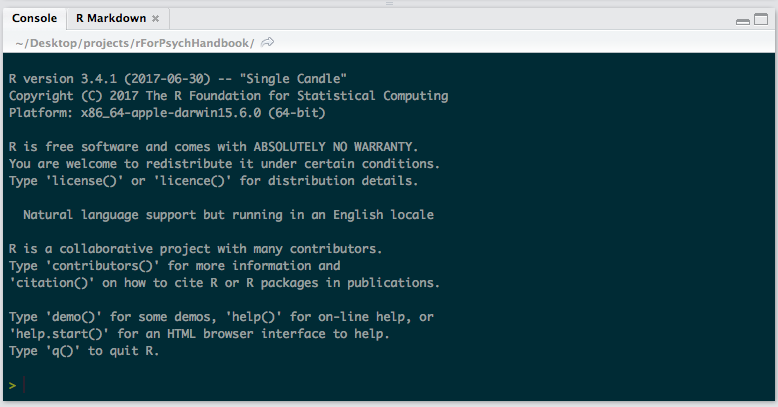
\includegraphics{img/setwdinr.png}
\caption{Current Working Directory Location}
\end{figure}

This whole book exists in a folder that lives in the projects folder on
my Desktop. If you're not familiar with how your computer is set up,
it's worth checking out an explanation or having someone walk you
through the hierarchy your computer's directories.

Once you have an basic understanding of this, you can find where you are
in R by using the \texttt{getwd()} function. If you need to change your
working directory at any point, the function is \texttt{setwd()}. While
it might seem a bit tedious to have to think about things like this
right away, by setting up analysis projects in a clean, and organized
way you are going to be saving yourself hours in the future.

So with that, open up a new R script, and for your first line set your
working directory to a folder where you are going to want to work out
of.

\section{The Basics}\label{the-basics}

With this script set up, we can now start to play around with R! This
chapter covers a few basic things:

\begin{itemize}
\tightlist
\item
  The rationale behind to writing scripts and code
\item
  R as Calculator
\item
  Data Structures
\item
  Manipulating Data
\item
  Tons of functions
\item
  Whirlwind tour of R for psychologists
\end{itemize}

The goals of this chapter are to:

\begin{itemize}
\tightlist
\item
  Learn Basics of R and RStudio
\item
  Practice concepts with simple examples
\item
  Familiarize with vast array of functions
\item
  Have vocabulary and ``R'' way to think about problem solving
\end{itemize}

\section{R as Calculator}\label{r-as-calculator}

The Console of R is where all the action happens. You can use it just
like you would use a calculator. Try to do some basic math operations in
it.

\begin{Shaded}
\begin{Highlighting}[]
\DecValTok{2} \OperatorTok{+}\StringTok{ }\DecValTok{2}
\end{Highlighting}
\end{Shaded}

\begin{verbatim}
## [1] 4
\end{verbatim}

\begin{Shaded}
\begin{Highlighting}[]
\DecValTok{5} \OperatorTok{-}\StringTok{ }\DecValTok{2}
\end{Highlighting}
\end{Shaded}

\begin{verbatim}
## [1] 3
\end{verbatim}

\begin{Shaded}
\begin{Highlighting}[]
\DecValTok{10} \OperatorTok{/}\StringTok{ }\DecValTok{4}
\end{Highlighting}
\end{Shaded}

\begin{verbatim}
## [1] 2.5
\end{verbatim}

\begin{Shaded}
\begin{Highlighting}[]
\DecValTok{9} \OperatorTok{*}\StringTok{ }\DecValTok{200}
\end{Highlighting}
\end{Shaded}

\begin{verbatim}
## [1] 1800
\end{verbatim}

\begin{Shaded}
\begin{Highlighting}[]
\KeywordTok{sqrt}\NormalTok{(}\DecValTok{81}\NormalTok{)}
\end{Highlighting}
\end{Shaded}

\begin{verbatim}
## [1] 9
\end{verbatim}

\begin{Shaded}
\begin{Highlighting}[]
\DecValTok{10} \OperatorTok{>}\StringTok{ }\DecValTok{4}
\end{Highlighting}
\end{Shaded}

\begin{verbatim}
## [1] TRUE
\end{verbatim}

\begin{Shaded}
\begin{Highlighting}[]
\DecValTok{2} \OperatorTok{<}\StringTok{ }\OperatorTok{-}\DecValTok{1}
\end{Highlighting}
\end{Shaded}

\begin{verbatim}
## [1] FALSE
\end{verbatim}

You don't always want to print your output and retype it in. Idea is to
be very lazy (efficient).

Save some math to an object with the \textless{}- operator, then
manipulate that.

\begin{Shaded}
\begin{Highlighting}[]
\NormalTok{foo <-}\StringTok{ }\DecValTok{2} \OperatorTok{*}\StringTok{ }\DecValTok{3}
\NormalTok{foo }\OperatorTok{*}\StringTok{ }\DecValTok{6}
\end{Highlighting}
\end{Shaded}

\begin{verbatim}
## [1] 36
\end{verbatim}

Notice what has popped up in your environment in RStudio!

Let's get more efficient.

\begin{Shaded}
\begin{Highlighting}[]
\NormalTok{yearsInGradSchool <-}\StringTok{ }\KeywordTok{c}\NormalTok{(}\DecValTok{2}\NormalTok{,}\DecValTok{1}\NormalTok{,}\DecValTok{4}\NormalTok{,}\DecValTok{5}\NormalTok{,}\DecValTok{6}\NormalTok{,}\DecValTok{7}\NormalTok{,}\DecValTok{3}\NormalTok{,}\DecValTok{2}\NormalTok{,}\DecValTok{4}\NormalTok{,}\DecValTok{5}\NormalTok{,}\DecValTok{3}\NormalTok{)}
\end{Highlighting}
\end{Shaded}

talk about the \texttt{c()} function.

\begin{Shaded}
\begin{Highlighting}[]
\NormalTok{yearsInGradSchool }\OperatorTok{*}\StringTok{ }\DecValTok{3}
\end{Highlighting}
\end{Shaded}

\begin{verbatim}
##  [1]  6  3 12 15 18 21  9  6 12 15  9
\end{verbatim}

Or this

\begin{Shaded}
\begin{Highlighting}[]
\NormalTok{yearsInGradSchool }\OperatorTok{-}\StringTok{ }\DecValTok{2}
\end{Highlighting}
\end{Shaded}

\begin{verbatim}
##  [1]  0 -1  2  3  4  5  1  0  2  3  1
\end{verbatim}

\begin{Shaded}
\begin{Highlighting}[]
\NormalTok{yearsInGradSchool }\OperatorTok{<}\StringTok{ }\DecValTok{2}
\end{Highlighting}
\end{Shaded}

\begin{verbatim}
##  [1] FALSE  TRUE FALSE FALSE FALSE FALSE FALSE FALSE FALSE FALSE FALSE
\end{verbatim}

\begin{Shaded}
\begin{Highlighting}[]
\KeywordTok{mean}\NormalTok{(yearsInGradSchool)}
\end{Highlighting}
\end{Shaded}

\begin{verbatim}
## [1] 3.818182
\end{verbatim}

\begin{Shaded}
\begin{Highlighting}[]
\KeywordTok{sd}\NormalTok{(yearsInGradSchool)}
\end{Highlighting}
\end{Shaded}

\begin{verbatim}
## [1] 1.834022
\end{verbatim}

\begin{Shaded}
\begin{Highlighting}[]
\KeywordTok{hist}\NormalTok{(yearsInGradSchool)}
\end{Highlighting}
\end{Shaded}

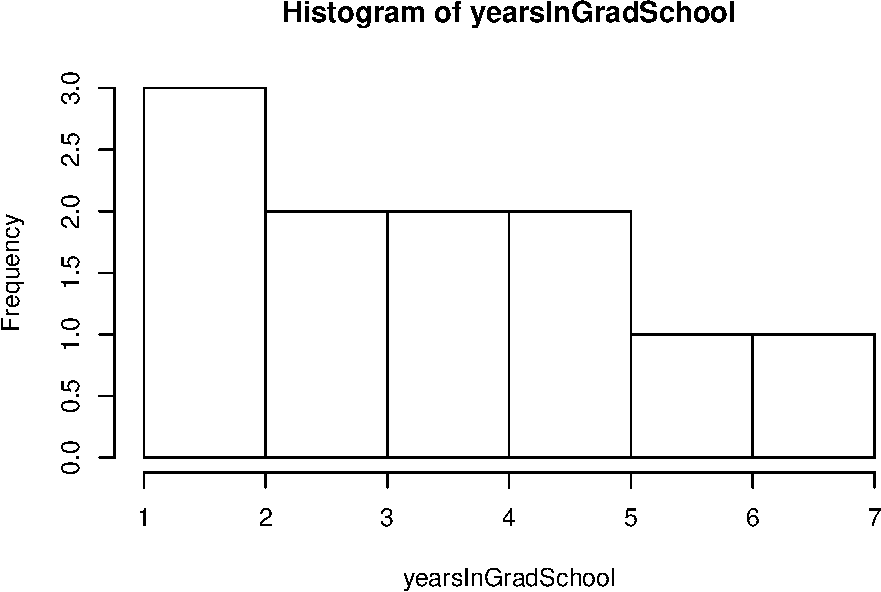
\includegraphics{bookdown-demo_files/figure-latex/unnamed-chunk-8-1.pdf}

\begin{Shaded}
\begin{Highlighting}[]
\KeywordTok{scale}\NormalTok{(yearsInGradSchool)}
\end{Highlighting}
\end{Shaded}

\begin{verbatim}
##              [,1]
##  [1,] -0.99136319
##  [2,] -1.53661295
##  [3,]  0.09913632
##  [4,]  0.64438608
##  [5,]  1.18963583
##  [6,]  1.73488559
##  [7,] -0.44611344
##  [8,] -0.99136319
##  [9,]  0.09913632
## [10,]  0.64438608
## [11,] -0.44611344
## attr(,"scaled:center")
## [1] 3.818182
## attr(,"scaled:scale")
## [1] 1.834022
\end{verbatim}

\begin{Shaded}
\begin{Highlighting}[]
\KeywordTok{range}\NormalTok{(yearsInGradSchool)}
\end{Highlighting}
\end{Shaded}

\begin{verbatim}
## [1] 1 7
\end{verbatim}

\begin{Shaded}
\begin{Highlighting}[]
\KeywordTok{min}\NormalTok{(yearsInGradSchool)}
\end{Highlighting}
\end{Shaded}

\begin{verbatim}
## [1] 1
\end{verbatim}

\begin{Shaded}
\begin{Highlighting}[]
\KeywordTok{class}\NormalTok{(yearsInGradSchool)}
\end{Highlighting}
\end{Shaded}

\begin{verbatim}
## [1] "numeric"
\end{verbatim}

\begin{Shaded}
\begin{Highlighting}[]
\KeywordTok{str}\NormalTok{(yearsInGradSchool)}
\end{Highlighting}
\end{Shaded}

\begin{verbatim}
##  num [1:11] 2 1 4 5 6 7 3 2 4 5 ...
\end{verbatim}

\begin{Shaded}
\begin{Highlighting}[]
\KeywordTok{summary}\NormalTok{(yearsInGradSchool)}
\end{Highlighting}
\end{Shaded}

\begin{verbatim}
##    Min. 1st Qu.  Median    Mean 3rd Qu.    Max. 
##   1.000   2.500   4.000   3.818   5.000   7.000
\end{verbatim}

\begin{Shaded}
\begin{Highlighting}[]
\NormalTok{yearsInGradSchool <-}\StringTok{ }\KeywordTok{c}\NormalTok{(}\DecValTok{2}\NormalTok{,}\DecValTok{1}\NormalTok{,}\DecValTok{4}\NormalTok{,}\DecValTok{5}\NormalTok{,}\DecValTok{6}\NormalTok{,}\DecValTok{7}\NormalTok{,}\DecValTok{3}\NormalTok{,}\DecValTok{2}\NormalTok{,}\DecValTok{4}\NormalTok{,}\DecValTok{5}\NormalTok{,}\DecValTok{3}\NormalTok{)}
\NormalTok{classesTaken <-}\StringTok{ }\KeywordTok{c}\NormalTok{(}\DecValTok{5}\NormalTok{,}\DecValTok{2}\NormalTok{,}\DecValTok{5}\NormalTok{,}\DecValTok{7}\NormalTok{,}\DecValTok{9}\NormalTok{,}\DecValTok{9}\NormalTok{,}\DecValTok{2}\NormalTok{,}\DecValTok{8}\NormalTok{,}\DecValTok{4}\NormalTok{,}\DecValTok{7}\NormalTok{,}\DecValTok{2}\NormalTok{)}
\NormalTok{gradData <-}\StringTok{ }\KeywordTok{data.frame}\NormalTok{(yearsInGradSchool,classesTaken)}
\end{Highlighting}
\end{Shaded}

\begin{Shaded}
\begin{Highlighting}[]
\KeywordTok{cor}\NormalTok{(yearsInGradSchool,classesTaken)}
\end{Highlighting}
\end{Shaded}

\begin{verbatim}
## [1] 0.6763509
\end{verbatim}

Basic plots, arguments. ggplot and libraries

\begin{Shaded}
\begin{Highlighting}[]
\KeywordTok{plot}\NormalTok{(yearsInGradSchool,classesTaken, }
     \DataTypeTok{data =}\NormalTok{ gradData, }
     \DataTypeTok{main =} \StringTok{"My Plot"}\NormalTok{, }
     \DataTypeTok{xlab =} \StringTok{"Years in Grad School"}\NormalTok{, }
     \DataTypeTok{ylab =} \StringTok{"Classes Taken"}\NormalTok{)}
\end{Highlighting}
\end{Shaded}

\begin{verbatim}
## Warning in plot.window(...): "data" is not a graphical parameter
\end{verbatim}

\begin{verbatim}
## Warning in plot.xy(xy, type, ...): "data" is not a graphical parameter
\end{verbatim}

\begin{verbatim}
## Warning in axis(side = side, at = at, labels = labels, ...): "data" is not
## a graphical parameter

## Warning in axis(side = side, at = at, labels = labels, ...): "data" is not
## a graphical parameter
\end{verbatim}

\begin{verbatim}
## Warning in box(...): "data" is not a graphical parameter
\end{verbatim}

\begin{verbatim}
## Warning in title(...): "data" is not a graphical parameter
\end{verbatim}

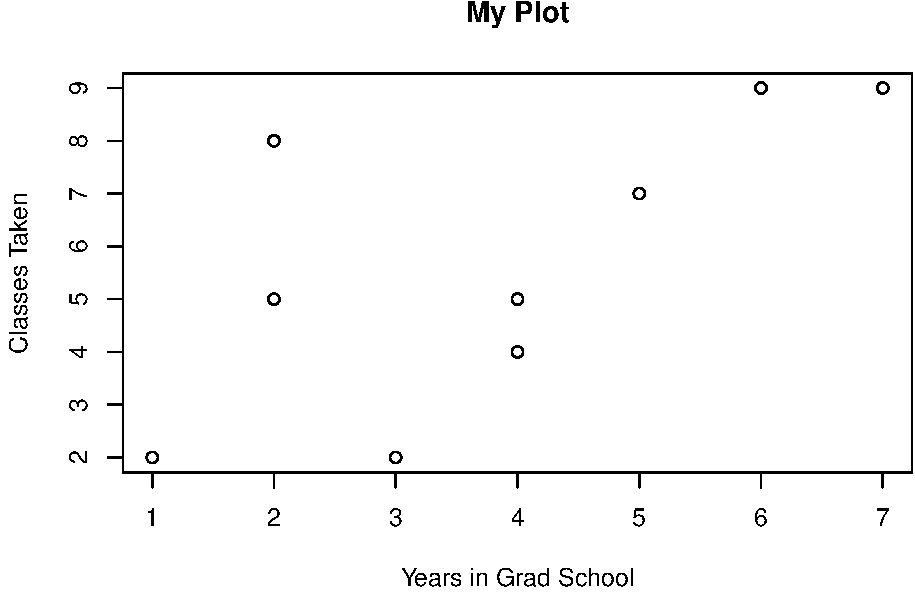
\includegraphics{bookdown-demo_files/figure-latex/unnamed-chunk-11-1.pdf}

\section{Data Exploration}\label{data-exploration}

\begin{Shaded}
\begin{Highlighting}[]
\KeywordTok{str}\NormalTok{(iris)}
\end{Highlighting}
\end{Shaded}

\begin{verbatim}
## 'data.frame':    150 obs. of  5 variables:
##  $ Sepal.Length: num  5.1 4.9 4.7 4.6 5 5.4 4.6 5 4.4 4.9 ...
##  $ Sepal.Width : num  3.5 3 3.2 3.1 3.6 3.9 3.4 3.4 2.9 3.1 ...
##  $ Petal.Length: num  1.4 1.4 1.3 1.5 1.4 1.7 1.4 1.5 1.4 1.5 ...
##  $ Petal.Width : num  0.2 0.2 0.2 0.2 0.2 0.4 0.3 0.2 0.2 0.1 ...
##  $ Species     : Factor w/ 3 levels "setosa","versicolor",..: 1 1 1 1 1 1 1 1 1 1 ...
\end{verbatim}

\begin{Shaded}
\begin{Highlighting}[]
\KeywordTok{class}\NormalTok{(iris)}
\end{Highlighting}
\end{Shaded}

\begin{verbatim}
## [1] "data.frame"
\end{verbatim}

\begin{Shaded}
\begin{Highlighting}[]
\KeywordTok{summary}\NormalTok{(iris)}
\end{Highlighting}
\end{Shaded}

\begin{verbatim}
##   Sepal.Length    Sepal.Width     Petal.Length    Petal.Width   
##  Min.   :4.300   Min.   :2.000   Min.   :1.000   Min.   :0.100  
##  1st Qu.:5.100   1st Qu.:2.800   1st Qu.:1.600   1st Qu.:0.300  
##  Median :5.800   Median :3.000   Median :4.350   Median :1.300  
##  Mean   :5.843   Mean   :3.057   Mean   :3.758   Mean   :1.199  
##  3rd Qu.:6.400   3rd Qu.:3.300   3rd Qu.:5.100   3rd Qu.:1.800  
##  Max.   :7.900   Max.   :4.400   Max.   :6.900   Max.   :2.500  
##        Species  
##  setosa    :50  
##  versicolor:50  
##  virginica :50  
##                 
##                 
## 
\end{verbatim}

Accessing individual `columns' is done with the \texttt{\$} operator

\begin{Shaded}
\begin{Highlighting}[]
\NormalTok{iris}\OperatorTok{$}\NormalTok{Sepal.Length}
\end{Highlighting}
\end{Shaded}

\begin{verbatim}
##   [1] 5.1 4.9 4.7 4.6 5.0 5.4 4.6 5.0 4.4 4.9 5.4 4.8 4.8 4.3 5.8 5.7 5.4
##  [18] 5.1 5.7 5.1 5.4 5.1 4.6 5.1 4.8 5.0 5.0 5.2 5.2 4.7 4.8 5.4 5.2 5.5
##  [35] 4.9 5.0 5.5 4.9 4.4 5.1 5.0 4.5 4.4 5.0 5.1 4.8 5.1 4.6 5.3 5.0 7.0
##  [52] 6.4 6.9 5.5 6.5 5.7 6.3 4.9 6.6 5.2 5.0 5.9 6.0 6.1 5.6 6.7 5.6 5.8
##  [69] 6.2 5.6 5.9 6.1 6.3 6.1 6.4 6.6 6.8 6.7 6.0 5.7 5.5 5.5 5.8 6.0 5.4
##  [86] 6.0 6.7 6.3 5.6 5.5 5.5 6.1 5.8 5.0 5.6 5.7 5.7 6.2 5.1 5.7 6.3 5.8
## [103] 7.1 6.3 6.5 7.6 4.9 7.3 6.7 7.2 6.5 6.4 6.8 5.7 5.8 6.4 6.5 7.7 7.7
## [120] 6.0 6.9 5.6 7.7 6.3 6.7 7.2 6.2 6.1 6.4 7.2 7.4 7.9 6.4 6.3 6.1 7.7
## [137] 6.3 6.4 6.0 6.9 6.7 6.9 5.8 6.8 6.7 6.7 6.3 6.5 6.2 5.9
\end{verbatim}

Can you use this to plot the different numeric values against each
other?

What would the follow commands do?

\begin{Shaded}
\begin{Highlighting}[]
\KeywordTok{hist}\NormalTok{(}\KeywordTok{scale}\NormalTok{(iris}\OperatorTok{$}\NormalTok{Sepal.Length))}
\end{Highlighting}
\end{Shaded}

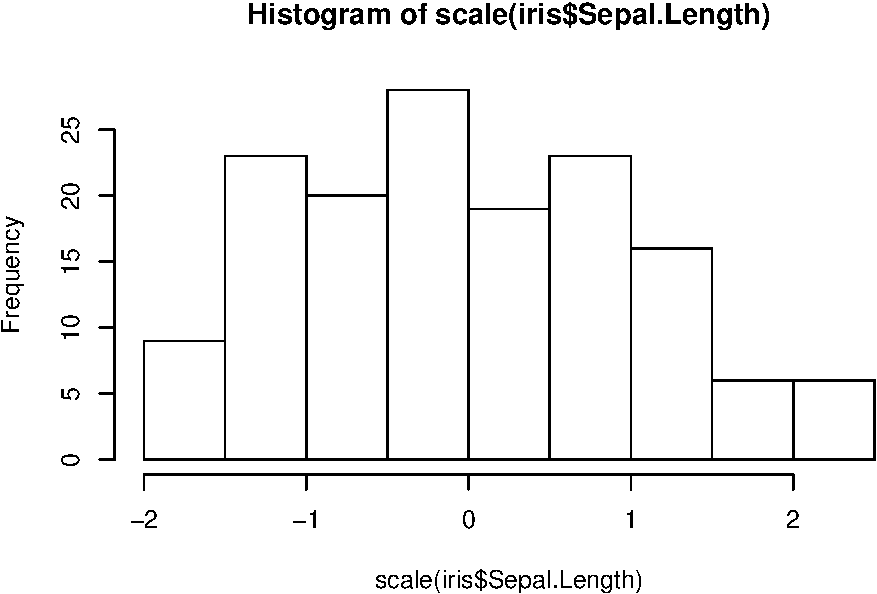
\includegraphics{bookdown-demo_files/figure-latex/unnamed-chunk-14-1.pdf}

\begin{Shaded}
\begin{Highlighting}[]
\NormalTok{iris}\OperatorTok{$}\NormalTok{Sepal.Length.scale <-}\StringTok{ }\KeywordTok{scale}\NormalTok{(iris}\OperatorTok{$}\NormalTok{Sepal.Length)}
\end{Highlighting}
\end{Shaded}

\section{Indexing}\label{indexing}

Let's combine logical indexing with creating new objects.

What do the follow commands do? Why?

\begin{Shaded}
\begin{Highlighting}[]
\NormalTok{iris[}\DecValTok{1}\NormalTok{,}\DecValTok{1}\NormalTok{]}
\end{Highlighting}
\end{Shaded}

\begin{verbatim}
## [1] 5.1
\end{verbatim}

\begin{Shaded}
\begin{Highlighting}[]
\NormalTok{iris[}\DecValTok{2}\NormalTok{,]}
\end{Highlighting}
\end{Shaded}

\begin{verbatim}
##   Sepal.Length Sepal.Width Petal.Length Petal.Width Species
## 2          4.9           3          1.4         0.2  setosa
##   Sepal.Length.scale
## 2            -1.1392
\end{verbatim}

\begin{Shaded}
\begin{Highlighting}[]
\NormalTok{iris[,}\DecValTok{5}\NormalTok{]}
\end{Highlighting}
\end{Shaded}

\begin{verbatim}
##   [1] setosa     setosa     setosa     setosa     setosa     setosa    
##   [7] setosa     setosa     setosa     setosa     setosa     setosa    
##  [13] setosa     setosa     setosa     setosa     setosa     setosa    
##  [19] setosa     setosa     setosa     setosa     setosa     setosa    
##  [25] setosa     setosa     setosa     setosa     setosa     setosa    
##  [31] setosa     setosa     setosa     setosa     setosa     setosa    
##  [37] setosa     setosa     setosa     setosa     setosa     setosa    
##  [43] setosa     setosa     setosa     setosa     setosa     setosa    
##  [49] setosa     setosa     versicolor versicolor versicolor versicolor
##  [55] versicolor versicolor versicolor versicolor versicolor versicolor
##  [61] versicolor versicolor versicolor versicolor versicolor versicolor
##  [67] versicolor versicolor versicolor versicolor versicolor versicolor
##  [73] versicolor versicolor versicolor versicolor versicolor versicolor
##  [79] versicolor versicolor versicolor versicolor versicolor versicolor
##  [85] versicolor versicolor versicolor versicolor versicolor versicolor
##  [91] versicolor versicolor versicolor versicolor versicolor versicolor
##  [97] versicolor versicolor versicolor versicolor virginica  virginica 
## [103] virginica  virginica  virginica  virginica  virginica  virginica 
## [109] virginica  virginica  virginica  virginica  virginica  virginica 
## [115] virginica  virginica  virginica  virginica  virginica  virginica 
## [121] virginica  virginica  virginica  virginica  virginica  virginica 
## [127] virginica  virginica  virginica  virginica  virginica  virginica 
## [133] virginica  virginica  virginica  virginica  virginica  virginica 
## [139] virginica  virginica  virginica  virginica  virginica  virginica 
## [145] virginica  virginica  virginica  virginica  virginica  virginica 
## Levels: setosa versicolor virginica
\end{verbatim}

\begin{Shaded}
\begin{Highlighting}[]
\NormalTok{iris[iris}\OperatorTok{$}\NormalTok{Sepal.Length }\OperatorTok{<}\StringTok{ }\DecValTok{5}\NormalTok{,]}
\end{Highlighting}
\end{Shaded}

\begin{verbatim}
##     Sepal.Length Sepal.Width Petal.Length Petal.Width    Species
## 2            4.9         3.0          1.4         0.2     setosa
## 3            4.7         3.2          1.3         0.2     setosa
## 4            4.6         3.1          1.5         0.2     setosa
## 7            4.6         3.4          1.4         0.3     setosa
## 9            4.4         2.9          1.4         0.2     setosa
## 10           4.9         3.1          1.5         0.1     setosa
## 12           4.8         3.4          1.6         0.2     setosa
## 13           4.8         3.0          1.4         0.1     setosa
## 14           4.3         3.0          1.1         0.1     setosa
## 23           4.6         3.6          1.0         0.2     setosa
## 25           4.8         3.4          1.9         0.2     setosa
## 30           4.7         3.2          1.6         0.2     setosa
## 31           4.8         3.1          1.6         0.2     setosa
## 35           4.9         3.1          1.5         0.2     setosa
## 38           4.9         3.6          1.4         0.1     setosa
## 39           4.4         3.0          1.3         0.2     setosa
## 42           4.5         2.3          1.3         0.3     setosa
## 43           4.4         3.2          1.3         0.2     setosa
## 46           4.8         3.0          1.4         0.3     setosa
## 48           4.6         3.2          1.4         0.2     setosa
## 58           4.9         2.4          3.3         1.0 versicolor
## 107          4.9         2.5          4.5         1.7  virginica
##     Sepal.Length.scale
## 2            -1.139200
## 3            -1.380727
## 4            -1.501490
## 7            -1.501490
## 9            -1.743017
## 10           -1.139200
## 12           -1.259964
## 13           -1.259964
## 14           -1.863780
## 23           -1.501490
## 25           -1.259964
## 30           -1.380727
## 31           -1.259964
## 35           -1.139200
## 38           -1.139200
## 39           -1.743017
## 42           -1.622254
## 43           -1.743017
## 46           -1.259964
## 48           -1.501490
## 58           -1.139200
## 107          -1.139200
\end{verbatim}

\begin{Shaded}
\begin{Highlighting}[]
\NormalTok{iris[,}\KeywordTok{c}\NormalTok{(}\DecValTok{1}\OperatorTok{:}\DecValTok{4}\NormalTok{)]}
\end{Highlighting}
\end{Shaded}

\begin{verbatim}
##     Sepal.Length Sepal.Width Petal.Length Petal.Width
## 1            5.1         3.5          1.4         0.2
## 2            4.9         3.0          1.4         0.2
## 3            4.7         3.2          1.3         0.2
## 4            4.6         3.1          1.5         0.2
## 5            5.0         3.6          1.4         0.2
## 6            5.4         3.9          1.7         0.4
## 7            4.6         3.4          1.4         0.3
## 8            5.0         3.4          1.5         0.2
## 9            4.4         2.9          1.4         0.2
## 10           4.9         3.1          1.5         0.1
## 11           5.4         3.7          1.5         0.2
## 12           4.8         3.4          1.6         0.2
## 13           4.8         3.0          1.4         0.1
## 14           4.3         3.0          1.1         0.1
## 15           5.8         4.0          1.2         0.2
## 16           5.7         4.4          1.5         0.4
## 17           5.4         3.9          1.3         0.4
## 18           5.1         3.5          1.4         0.3
## 19           5.7         3.8          1.7         0.3
## 20           5.1         3.8          1.5         0.3
## 21           5.4         3.4          1.7         0.2
## 22           5.1         3.7          1.5         0.4
## 23           4.6         3.6          1.0         0.2
## 24           5.1         3.3          1.7         0.5
## 25           4.8         3.4          1.9         0.2
## 26           5.0         3.0          1.6         0.2
## 27           5.0         3.4          1.6         0.4
## 28           5.2         3.5          1.5         0.2
## 29           5.2         3.4          1.4         0.2
## 30           4.7         3.2          1.6         0.2
## 31           4.8         3.1          1.6         0.2
## 32           5.4         3.4          1.5         0.4
## 33           5.2         4.1          1.5         0.1
## 34           5.5         4.2          1.4         0.2
## 35           4.9         3.1          1.5         0.2
## 36           5.0         3.2          1.2         0.2
## 37           5.5         3.5          1.3         0.2
## 38           4.9         3.6          1.4         0.1
## 39           4.4         3.0          1.3         0.2
## 40           5.1         3.4          1.5         0.2
## 41           5.0         3.5          1.3         0.3
## 42           4.5         2.3          1.3         0.3
## 43           4.4         3.2          1.3         0.2
## 44           5.0         3.5          1.6         0.6
## 45           5.1         3.8          1.9         0.4
## 46           4.8         3.0          1.4         0.3
## 47           5.1         3.8          1.6         0.2
## 48           4.6         3.2          1.4         0.2
## 49           5.3         3.7          1.5         0.2
## 50           5.0         3.3          1.4         0.2
## 51           7.0         3.2          4.7         1.4
## 52           6.4         3.2          4.5         1.5
## 53           6.9         3.1          4.9         1.5
## 54           5.5         2.3          4.0         1.3
## 55           6.5         2.8          4.6         1.5
## 56           5.7         2.8          4.5         1.3
## 57           6.3         3.3          4.7         1.6
## 58           4.9         2.4          3.3         1.0
## 59           6.6         2.9          4.6         1.3
## 60           5.2         2.7          3.9         1.4
## 61           5.0         2.0          3.5         1.0
## 62           5.9         3.0          4.2         1.5
## 63           6.0         2.2          4.0         1.0
## 64           6.1         2.9          4.7         1.4
## 65           5.6         2.9          3.6         1.3
## 66           6.7         3.1          4.4         1.4
## 67           5.6         3.0          4.5         1.5
## 68           5.8         2.7          4.1         1.0
## 69           6.2         2.2          4.5         1.5
## 70           5.6         2.5          3.9         1.1
## 71           5.9         3.2          4.8         1.8
## 72           6.1         2.8          4.0         1.3
## 73           6.3         2.5          4.9         1.5
## 74           6.1         2.8          4.7         1.2
## 75           6.4         2.9          4.3         1.3
## 76           6.6         3.0          4.4         1.4
## 77           6.8         2.8          4.8         1.4
## 78           6.7         3.0          5.0         1.7
## 79           6.0         2.9          4.5         1.5
## 80           5.7         2.6          3.5         1.0
## 81           5.5         2.4          3.8         1.1
## 82           5.5         2.4          3.7         1.0
## 83           5.8         2.7          3.9         1.2
## 84           6.0         2.7          5.1         1.6
## 85           5.4         3.0          4.5         1.5
## 86           6.0         3.4          4.5         1.6
## 87           6.7         3.1          4.7         1.5
## 88           6.3         2.3          4.4         1.3
## 89           5.6         3.0          4.1         1.3
## 90           5.5         2.5          4.0         1.3
## 91           5.5         2.6          4.4         1.2
## 92           6.1         3.0          4.6         1.4
## 93           5.8         2.6          4.0         1.2
## 94           5.0         2.3          3.3         1.0
## 95           5.6         2.7          4.2         1.3
## 96           5.7         3.0          4.2         1.2
## 97           5.7         2.9          4.2         1.3
## 98           6.2         2.9          4.3         1.3
## 99           5.1         2.5          3.0         1.1
## 100          5.7         2.8          4.1         1.3
## 101          6.3         3.3          6.0         2.5
## 102          5.8         2.7          5.1         1.9
## 103          7.1         3.0          5.9         2.1
## 104          6.3         2.9          5.6         1.8
## 105          6.5         3.0          5.8         2.2
## 106          7.6         3.0          6.6         2.1
## 107          4.9         2.5          4.5         1.7
## 108          7.3         2.9          6.3         1.8
## 109          6.7         2.5          5.8         1.8
## 110          7.2         3.6          6.1         2.5
## 111          6.5         3.2          5.1         2.0
## 112          6.4         2.7          5.3         1.9
## 113          6.8         3.0          5.5         2.1
## 114          5.7         2.5          5.0         2.0
## 115          5.8         2.8          5.1         2.4
## 116          6.4         3.2          5.3         2.3
## 117          6.5         3.0          5.5         1.8
## 118          7.7         3.8          6.7         2.2
## 119          7.7         2.6          6.9         2.3
## 120          6.0         2.2          5.0         1.5
## 121          6.9         3.2          5.7         2.3
## 122          5.6         2.8          4.9         2.0
## 123          7.7         2.8          6.7         2.0
## 124          6.3         2.7          4.9         1.8
## 125          6.7         3.3          5.7         2.1
## 126          7.2         3.2          6.0         1.8
## 127          6.2         2.8          4.8         1.8
## 128          6.1         3.0          4.9         1.8
## 129          6.4         2.8          5.6         2.1
## 130          7.2         3.0          5.8         1.6
## 131          7.4         2.8          6.1         1.9
## 132          7.9         3.8          6.4         2.0
## 133          6.4         2.8          5.6         2.2
## 134          6.3         2.8          5.1         1.5
## 135          6.1         2.6          5.6         1.4
## 136          7.7         3.0          6.1         2.3
## 137          6.3         3.4          5.6         2.4
## 138          6.4         3.1          5.5         1.8
## 139          6.0         3.0          4.8         1.8
## 140          6.9         3.1          5.4         2.1
## 141          6.7         3.1          5.6         2.4
## 142          6.9         3.1          5.1         2.3
## 143          5.8         2.7          5.1         1.9
## 144          6.8         3.2          5.9         2.3
## 145          6.7         3.3          5.7         2.5
## 146          6.7         3.0          5.2         2.3
## 147          6.3         2.5          5.0         1.9
## 148          6.5         3.0          5.2         2.0
## 149          6.2         3.4          5.4         2.3
## 150          5.9         3.0          5.1         1.8
\end{verbatim}

\begin{Shaded}
\begin{Highlighting}[]
\NormalTok{iris[}\KeywordTok{c}\NormalTok{(}\DecValTok{1}\NormalTok{,}\DecValTok{2}\NormalTok{,}\DecValTok{3}\NormalTok{,}\DecValTok{4}\NormalTok{,}\DecValTok{5}\NormalTok{,}\DecValTok{6}\NormalTok{,}\DecValTok{8}\NormalTok{),}\KeywordTok{c}\NormalTok{(}\DecValTok{1}\OperatorTok{:}\DecValTok{3}\NormalTok{,}\DecValTok{5}\NormalTok{)]}
\end{Highlighting}
\end{Shaded}

\begin{verbatim}
##   Sepal.Length Sepal.Width Petal.Length Species
## 1          5.1         3.5          1.4  setosa
## 2          4.9         3.0          1.4  setosa
## 3          4.7         3.2          1.3  setosa
## 4          4.6         3.1          1.5  setosa
## 5          5.0         3.6          1.4  setosa
## 6          5.4         3.9          1.7  setosa
## 8          5.0         3.4          1.5  setosa
\end{verbatim}

\begin{Shaded}
\begin{Highlighting}[]
\NormalTok{Setosas <-}\StringTok{ }\NormalTok{iris[iris}\OperatorTok{$}\NormalTok{Species }\OperatorTok{==}\StringTok{ "setosa"}\NormalTok{,]}
\end{Highlighting}
\end{Shaded}

This could be an entire lecture by itself!!!

\section{Whirlwind Tour of R}\label{whirlwind-tour-of-r}

R's power comes in the fact that you download packages to put on top of
base R

\begin{itemize}
\tightlist
\item
  Turning Data tables into already formatted APA Latex Tables
  (stargazer, xtable)
\item
  Creating Publication Quality Graphs (ggplot2)
\item
  Text manipulation (stringr)
\item
  Exploring data and not making chart after chart after chart (psych)
\item
  Every statistical test you could want (psych, cars, ezanova, lavaan)
\item
  Software to plot not so normal output (SEMplots)
\item
  Making Websites in R
\item
  These slides were written in R
\item
  Quickly processing huge datasets (data.table, dplyr)
\item
  Tons of Machine Learning
\end{itemize}

\begin{Shaded}
\begin{Highlighting}[]
\KeywordTok{library}\NormalTok{(ggplot2)}
\KeywordTok{ggplot}\NormalTok{(iris, }\KeywordTok{aes}\NormalTok{(}\DataTypeTok{x =}\NormalTok{ Sepal.Length, }\DataTypeTok{y =}\NormalTok{ Sepal.Width, }
                 \DataTypeTok{color =}\NormalTok{ Species), }
       \DataTypeTok{xlab =} \StringTok{"Sepal Length"}\NormalTok{,}
       \DataTypeTok{ylab =} \StringTok{"Sepal Width"}\NormalTok{,}
       \DataTypeTok{main =} \StringTok{"My Plot"}\NormalTok{) }\OperatorTok{+}\StringTok{ }\KeywordTok{geom_point}\NormalTok{()}
\end{Highlighting}
\end{Shaded}

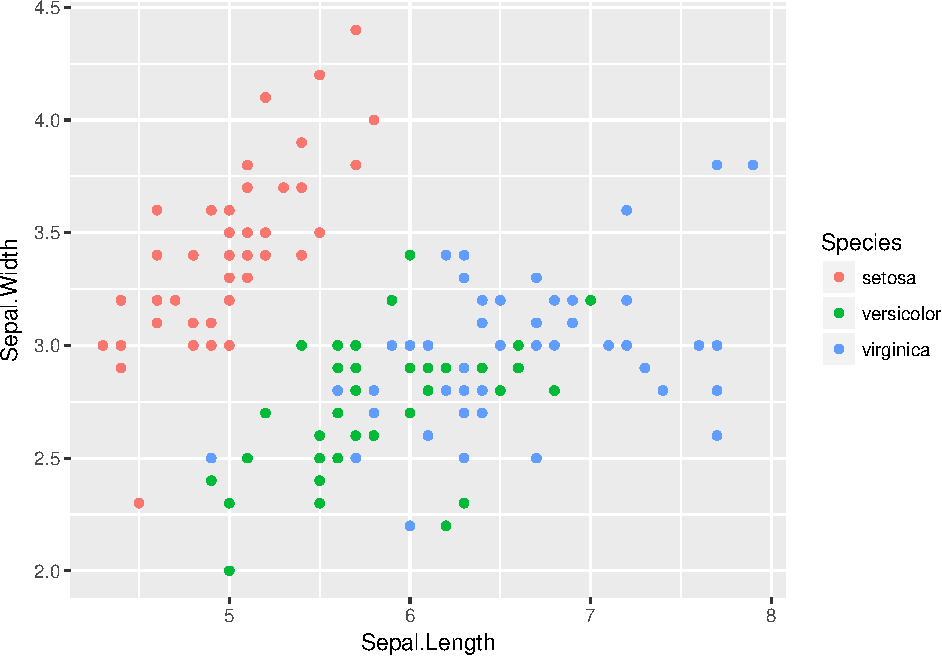
\includegraphics{bookdown-demo_files/figure-latex/unnamed-chunk-16-1.pdf}

Or stuff for data exploration

\begin{Shaded}
\begin{Highlighting}[]
\KeywordTok{library}\NormalTok{(psych)}
\end{Highlighting}
\end{Shaded}

\begin{verbatim}
## Warning: package 'psych' was built under R version 3.4.4
\end{verbatim}

\begin{verbatim}
## 
## Attaching package: 'psych'
\end{verbatim}

\begin{verbatim}
## The following objects are masked from 'package:ggplot2':
## 
##     %+%, alpha
\end{verbatim}

\begin{Shaded}
\begin{Highlighting}[]
\KeywordTok{pairs.panels}\NormalTok{(iris)}
\end{Highlighting}
\end{Shaded}

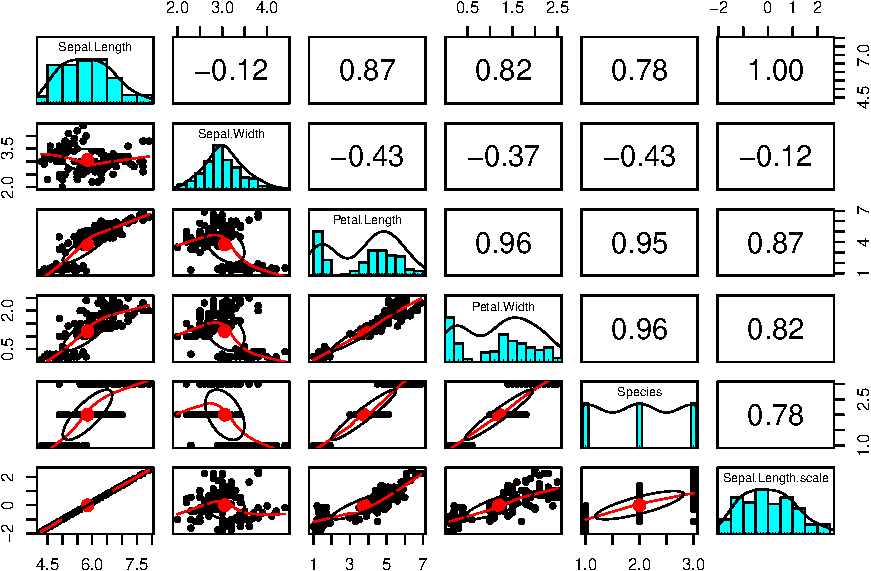
\includegraphics{bookdown-demo_files/figure-latex/unnamed-chunk-17-1.pdf}

\section{Functions for Psychologists}\label{functions-for-psychologists}

\begin{itemize}
\tightlist
\item
  \texttt{nlme()} and \texttt{lme4()} for Multilevel Modeling
\item
  \texttt{lavaan()} for Latent Variable Analysis
\item
  \texttt{ezAnova()} for ANOVA based testing; the anova() function does
  model comparisons
\item
  profileR for Repeated Measures MANOVA
\item
  \texttt{glm()} and \texttt{lm()} for linear models
\item
  \texttt{caret()} for Machine Learning
\end{itemize}

\section{Resources}\label{resources}

\begin{itemize}
\tightlist
\item
  swirl
\item
  \href{www.stackoverflow.com}{stackoverflow.com}
\item
  Twitter
\item
  Your peers
\item
  R Community
\end{itemize}

\subsection{Template Stuff}\label{template-stuff}

You can label chapter and section titles using \texttt{\{\#label\}}
after them, e.g., we can reference Chapter \ref{intro}. If you do not
manually label them, there will be automatic labels anyway, e.g.,
Chapter \ref{methods}.

Figures and tables with captions will be placed in \texttt{figure} and
\texttt{table} environments, respectively.

\begin{Shaded}
\begin{Highlighting}[]
\KeywordTok{par}\NormalTok{(}\DataTypeTok{mar =} \KeywordTok{c}\NormalTok{(}\DecValTok{4}\NormalTok{, }\DecValTok{4}\NormalTok{, .}\DecValTok{1}\NormalTok{, .}\DecValTok{1}\NormalTok{))}
\KeywordTok{plot}\NormalTok{(pressure, }\DataTypeTok{type =} \StringTok{'b'}\NormalTok{, }\DataTypeTok{pch =} \DecValTok{19}\NormalTok{)}
\end{Highlighting}
\end{Shaded}

\begin{figure}

{\centering 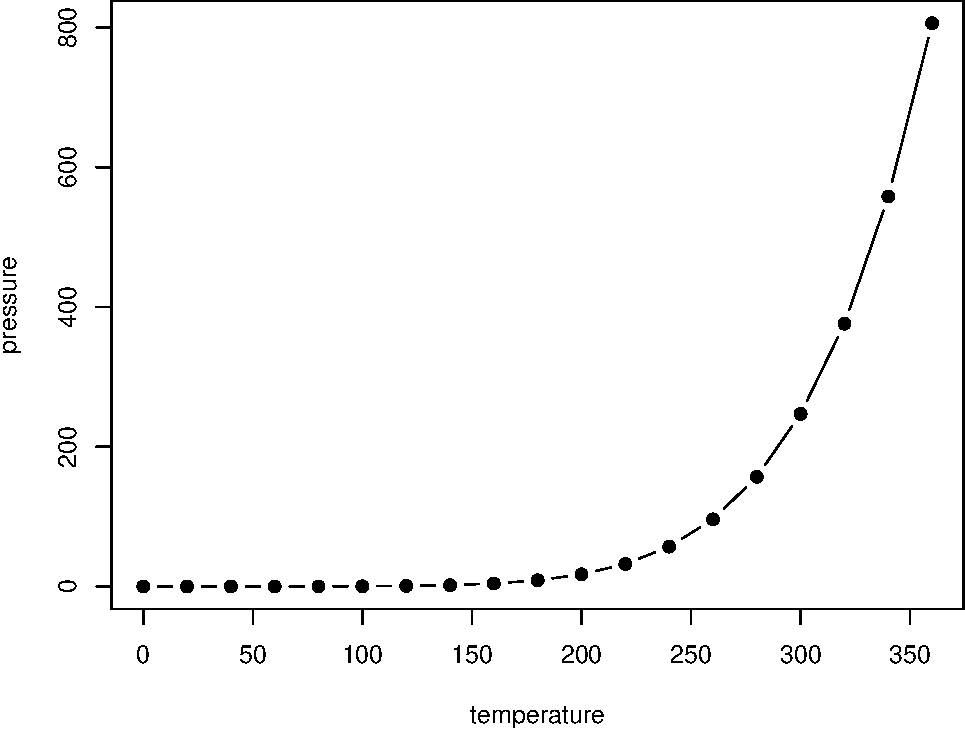
\includegraphics[width=0.8\linewidth]{bookdown-demo_files/figure-latex/nice-fig-1} 

}

\caption{Here is a nice figure!}\label{fig:nice-fig}
\end{figure}

Reference a figure by its code chunk label with the \texttt{fig:}
prefix, e.g., see Figure \ref{fig:nice-fig}. Similarly, you can
reference tables generated from \texttt{knitr::kable()}, e.g., see Table
\ref{tab:nice-tab}.

\begin{Shaded}
\begin{Highlighting}[]
\NormalTok{knitr}\OperatorTok{::}\KeywordTok{kable}\NormalTok{(}
  \KeywordTok{head}\NormalTok{(iris, }\DecValTok{20}\NormalTok{), }\DataTypeTok{caption =} \StringTok{'Here is a nice table!'}\NormalTok{,}
  \DataTypeTok{booktabs =} \OtherTok{TRUE}
\NormalTok{)}
\end{Highlighting}
\end{Shaded}

\begin{table}

\caption{\label{tab:nice-tab}Here is a nice table!}
\centering
\begin{tabular}[t]{rrrrlr}
\toprule
Sepal.Length & Sepal.Width & Petal.Length & Petal.Width & Species & Sepal.Length.scale\\
\midrule
5.1 & 3.5 & 1.4 & 0.2 & setosa & -0.89767388\\
4.9 & 3.0 & 1.4 & 0.2 & setosa & -1.13920048\\
4.7 & 3.2 & 1.3 & 0.2 & setosa & -1.38072709\\
4.6 & 3.1 & 1.5 & 0.2 & setosa & -1.50149039\\
5.0 & 3.6 & 1.4 & 0.2 & setosa & -1.01843718\\
\addlinespace
5.4 & 3.9 & 1.7 & 0.4 & setosa & -0.53538397\\
4.6 & 3.4 & 1.4 & 0.3 & setosa & -1.50149039\\
5.0 & 3.4 & 1.5 & 0.2 & setosa & -1.01843718\\
4.4 & 2.9 & 1.4 & 0.2 & setosa & -1.74301699\\
4.9 & 3.1 & 1.5 & 0.1 & setosa & -1.13920048\\
\addlinespace
5.4 & 3.7 & 1.5 & 0.2 & setosa & -0.53538397\\
4.8 & 3.4 & 1.6 & 0.2 & setosa & -1.25996379\\
4.8 & 3.0 & 1.4 & 0.1 & setosa & -1.25996379\\
4.3 & 3.0 & 1.1 & 0.1 & setosa & -1.86378030\\
5.8 & 4.0 & 1.2 & 0.2 & setosa & -0.05233076\\
\addlinespace
5.7 & 4.4 & 1.5 & 0.4 & setosa & -0.17309407\\
5.4 & 3.9 & 1.3 & 0.4 & setosa & -0.53538397\\
5.1 & 3.5 & 1.4 & 0.3 & setosa & -0.89767388\\
5.7 & 3.8 & 1.7 & 0.3 & setosa & -0.17309407\\
5.1 & 3.8 & 1.5 & 0.3 & setosa & -0.89767388\\
\bottomrule
\end{tabular}
\end{table}

You can write citations, too. For example, we are using the
\textbf{bookdown} package \citep{R-bookdown} in this sample book, which
was built on top of R Markdown and \textbf{knitr} \citep{xie2015}.

\chapter{Data Manipulation in R}\label{data-manipulation-in-r}

This chapter will take you through a brief walk through of cleaning some
data in R. When starting out with R, it's not important that you
memorize every command and learn every line, but rather that you start
to think about how a computer programmer would solve a question (you!)
rather than get an undergrad RA to fix it by hand.

The first thing that you want to do to any script is to put a header on
it. It should cover a few things such as

\begin{itemize}
\tightlist
\item
  A Title
\item
  Who wrote the script?
\item
  When did you edit it last?
\item
  What does it do?
\item
  How does it work?
\item
  Does it take anything in specific?
\end{itemize}

The more information you can provide, the better. Remember that
6-Month-From-You now is going to be either your best or worst
collaborator.

Each script in R out to follow a general pattern. First list out some
information about it, then load in your libraries, and then set your
working directory and load your data.

\begin{Shaded}
\begin{Highlighting}[]
 \CommentTok{# Import Libraries }
 \KeywordTok{library}\NormalTok{(stringr)}
\end{Highlighting}
\end{Shaded}

\begin{verbatim}
## Warning: package 'stringr' was built under R version 3.4.3
\end{verbatim}

\begin{Shaded}
\begin{Highlighting}[]
 \KeywordTok{library}\NormalTok{(data.table)}
\end{Highlighting}
\end{Shaded}

\begin{verbatim}
## Warning: package 'data.table' was built under R version 3.4.2
\end{verbatim}

\begin{Shaded}
\begin{Highlighting}[]
 \KeywordTok{library}\NormalTok{(psych)}
\end{Highlighting}
\end{Shaded}

Next thing you would do is set your working directory and load in your
data. Note here that you need to tell R exactly where to look!

\begin{Shaded}
\begin{Highlighting}[]
\CommentTok{# Make sure to load in both datasets as we will want them both in our analysis.}
\CommentTok{# We also want to make sure to clean both datasets as we are going. }
\NormalTok{experiment.data <-}\StringTok{ }\KeywordTok{read.csv}\NormalTok{(}\StringTok{"datasets/Demographic_Data.csv"}\NormalTok{)}
\NormalTok{item.level.data <-}\StringTok{ }\KeywordTok{read.csv}\NormalTok{(}\StringTok{"datasets/ItemLevelData.csv"}\NormalTok{)}
\end{Highlighting}
\end{Shaded}

You can also import data using RStudio's `Import Data' function in the
top right corner.

\begin{figure}
\centering
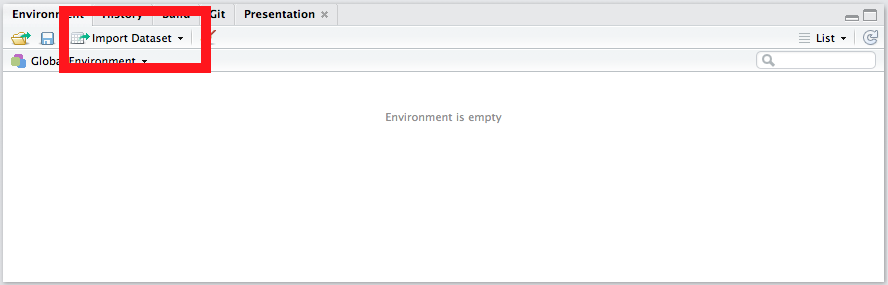
\includegraphics{img/importdatagui.png}
\caption{Import Data via RStudio's GUI}
\end{figure}

If you do do that, make sure to add in any of the libraries and code in
your script that is printed out below in RStudio's consle!

Next you should familiarize yourself with what your data looks like. Not
only do you have to be cautious of the shape of your data (wide
vs.~long), but there are a few different types of data that R uses in
its functionality.

Looking at the dataset from this experiment, we see lots of different
types of data listed. R did its best to guess what `kind' of data each
one is, but sometimes you have to change data types.

\begin{Shaded}
\begin{Highlighting}[]
\KeywordTok{str}\NormalTok{(experiment.data) }\CommentTok{# Check to see if R guessed correctly on data types}
\end{Highlighting}
\end{Shaded}

\begin{verbatim}
## 'data.frame':    251 obs. of  67 variables:
##  $ Sub               : int  10 11 12 13 14 15 16 17 18 19 ...
##  $ ACTIVE            : int  38 37 39 33 48 47 55 42 36 36 ...
##  $ PERCEPTUAL        : int  47 47 49 42 57 55 60 61 43 36 ...
##  $ MUSICAL           : int  28 16 21 26 7 8 46 39 19 24 ...
##  $ SINGING           : int  33 22 40 19 24 24 45 25 29 28 ...
##  $ EMOTIONS          : int  39 32 30 34 35 36 42 41 33 24 ...
##  $ GENERAL           : int  75 67 82 68 60 65 118 86 69 68 ...
##  $ inst              : Factor w/ 70 levels "","air drums",..: 9 4 67 46 28 36 36 36 48 28 ...
##  $ Age               : int  29 22 19 23 23 19 19 21 19 21 ...
##  $ Gender            : Factor w/ 13 levels "","COUNTRY","f",..: 6 6 6 12 12 4 6 4 12 10 ...
##  $ Major             : Factor w/ 147 levels "","AGRIBUSINESS",..: 24 126 38 88 67 79 95 17 143 47 ...
##  $ Minor             : Factor w/ 65 levels ""," Economics",..: 29 NA 50 NA 4 NA NA NA NA 39 ...
##  $ SchoolUGorG       : int  1 1 1 1 1 1 1 1 1 1 ...
##  $ MuscMajMinor      : int  1 1 1 1 1 1 2 1 1 1 ...
##  $ BeginTrain        : Factor w/ 20 levels "","10","11","12",..: 20 2 2 3 1 1 19 16 4 16 ...
##  $ AbsPitch          : Factor w/ 7 levels "","no","No","NO",..: 4 2 4 4 4 4 2 4 4 2 ...
##  $ YearsPrac         : int  4 1 3 7 0 0 11 7 2 6 ...
##  $ PeakPrac          : int  5 2 1 1 0 0 3 2 2 1 ...
##  $ Live12Mo          : Factor w/ 23 levels "","0","1","10",..: 9 15 3 2 20 9 17 12 14 18 ...
##  $ TheoryTrain       : int  4 0 0 0 0 0 4 4 0 0 ...
##  $ FormalYrs         : int  4 1 3 7 0 0 11 8 2 2 ...
##  $ NoOfInst          : int  1 0 1 2 0 0 5 1 1 0 ...
##  $ ActListenMin      : Factor w/ 34 levels "","0","1","10",..: 30 30 9 24 5 30 9 24 24 22 ...
##  $ SubjectNo         : int  10 11 12 13 14 15 16 17 18 19 ...
##  $ SubRaven          : int  10 11 12 13 14 15 16 17 18 19 ...
##  $ RavenB1           : int  10 7 3 10 7 6 8 8 4 3 ...
##  $ RavenB2           : int  8 10 7 10 8 10 9 10 6 3 ...
##  $ RavenB3           : int  10 6 7 11 5 6 8 8 5 3 ...
##  $ RavenTotal        : int  28 23 17 31 20 22 25 26 15 9 ...
##  $ OspanSub          : int  10 11 12 13 14 15 16 17 18 19 ...
##  $ OspanAccError     : int  8 7 7 1 2 12 4 8 5 37 ...
##  $ OspanMathError    : int  12 12 7 2 2 15 4 8 8 37 ...
##  $ OspanAbsoluteScore: int  29 20 48 68 33 20 68 36 16 14 ...
##  $ OspanPartialScore : int  47 41 65 73 50 44 70 64 30 23 ...
##  $ OspanB1           : int  21 11 21 25 17 14 25 19 10 8 ...
##  $ OspanB2           : int  14 18 23 23 16 17 20 24 11 6 ...
##  $ OspanB3           : int  12 12 21 25 17 13 25 21 9 9 ...
##  $ OspanSpeedErrTot  : int  4 5 0 1 0 3 0 0 3 0 ...
##  $ SymSub            : int  10 11 12 13 14 15 16 17 18 19 ...
##  $ SymAccErrTot      : int  1 4 2 1 0 4 2 3 2 23 ...
##  $ SymSpeedErrTot    : int  0 1 0 0 0 1 0 0 0 0 ...
##  $ SspanAbsScore     : int  10 15 21 27 15 9 30 24 12 18 ...
##  $ SspanPartiaScore  : int  19 29 34 34 26 25 38 30 18 24 ...
##  $ SspanB1           : int  8 11 10 13 8 9 13 7 8 8 ...
##  $ SspanB2           : int  4 13 13 10 8 10 14 14 4 7 ...
##  $ SspanB3           : int  7 5 11 11 10 6 11 9 6 9 ...
##  $ SymmErrTot        : int  1 5 2 1 0 5 2 3 2 23 ...
##  $ ToneSub           : int  10 11 12 13 14 15 16 17 18 19 ...
##  $ ToneAccErrTot     : int  8 5 8 1 4 7 3 6 3 36 ...
##  $ ToneMathErrTot    : int  9 5 8 2 5 10 5 6 6 38 ...
##  $ TspanAbsScore     : int  9 21 27 37 10 4 23 14 3 0 ...
##  $ TspanPartScore    : int  36 47 55 63 31 34 58 48 37 26 ...
##  $ TspanB1           : int  13 14 17 20 8 9 20 12 9 9 ...
##  $ TspanB2           : int  6 19 21 22 9 12 19 18 12 5 ...
##  $ TspanB3           : int  17 14 17 21 14 13 19 18 16 12 ...
##  $ ToneSpeedErrTot   : int  1 0 0 1 1 3 2 0 3 2 ...
##  $ BeatSub           : int  10 11 12 13 14 15 16 17 18 19 ...
##  $ BeatTotal         : int  11 10 14 13 14 10 14 11 7 12 ...
##  $ BeatAcc           : num  0.61 0.56 0.78 0.72 0.78 0.56 0.78 0.61 0.39 0.67 ...
##  $ MelodicSub        : int  10 11 12 13 14 15 16 17 18 19 ...
##  $ MelodicTot        : int  7 7 6 10 5 5 6 7 7 7 ...
##  $ MelodicAcc        : num  0.54 0.54 0.46 0.77 0.38 0.38 0.46 0.54 0.54 0.54 ...
##  $ Native            : int  1 1 1 1 1 1 1 2 1 1 ...
##  $ Paid              : int  1 1 1 1 1 1 1 1 1 1 ...
##  $ jv_NoGMSI         : int  0 0 0 0 0 0 0 0 0 0 ...
##  $ jv_nonNative      : int  0 0 0 0 0 0 0 1 0 0 ...
##  $ jv_noOspan        : int  0 0 0 0 0 0 0 0 0 0 ...
\end{verbatim}

Using \texttt{read.csv()} with its default setting, R had a couple of
bad guesses on variables we might need. We will have to reassign the
variable types or else we'll run into trouble later. In R we use factor
for grouping and analysis, best practice is to not set it as that until
you are OK with the format. It's easist to manipulate a character or
string. There are much more elegant ways to do this, but just to make a
point, I've gone through and fixed each one manually.

Notice how the output of \texttt{str()} has changed.

\begin{Shaded}
\begin{Highlighting}[]
\NormalTok{experiment.data}\OperatorTok{$}\NormalTok{inst <-}\StringTok{ }\KeywordTok{as.character}\NormalTok{(experiment.data}\OperatorTok{$}\NormalTok{inst)}
\NormalTok{experiment.data}\OperatorTok{$}\NormalTok{Gender <-}\StringTok{ }\KeywordTok{as.character}\NormalTok{(experiment.data}\OperatorTok{$}\NormalTok{Gender)}
\NormalTok{experiment.data}\OperatorTok{$}\NormalTok{Major <-}\StringTok{ }\KeywordTok{as.character}\NormalTok{(experiment.data}\OperatorTok{$}\NormalTok{Major)}
\NormalTok{experiment.data}\OperatorTok{$}\NormalTok{Minor <-}\StringTok{ }\KeywordTok{as.character}\NormalTok{(experiment.data}\OperatorTok{$}\NormalTok{Minor)}
\NormalTok{experiment.data}\OperatorTok{$}\NormalTok{BeginTrain <-}\StringTok{ }\KeywordTok{as.character}\NormalTok{(experiment.data}\OperatorTok{$}\NormalTok{BeginTrain)}
\NormalTok{experiment.data}\OperatorTok{$}\NormalTok{AbsPitch <-}\StringTok{ }\KeywordTok{as.character}\NormalTok{(experiment.data}\OperatorTok{$}\NormalTok{AbsPitch)}
\NormalTok{experiment.data}\OperatorTok{$}\NormalTok{Live12Mo <-}\StringTok{ }\KeywordTok{as.numeric}\NormalTok{(experiment.data}\OperatorTok{$}\NormalTok{Live12Mo)}
\NormalTok{experiment.data}\OperatorTok{$}\NormalTok{ActListenMin <-}\StringTok{ }\KeywordTok{as.character}\NormalTok{(experiment.data}\OperatorTok{$}\NormalTok{ActListenMin)}

\KeywordTok{str}\NormalTok{(experiment.data) }\CommentTok{# Notice how that our character columns now have " " around them.}
\end{Highlighting}
\end{Shaded}

\begin{verbatim}
## 'data.frame':    251 obs. of  67 variables:
##  $ Sub               : int  10 11 12 13 14 15 16 17 18 19 ...
##  $ ACTIVE            : int  38 37 39 33 48 47 55 42 36 36 ...
##  $ PERCEPTUAL        : int  47 47 49 42 57 55 60 61 43 36 ...
##  $ MUSICAL           : int  28 16 21 26 7 8 46 39 19 24 ...
##  $ SINGING           : int  33 22 40 19 24 24 45 25 29 28 ...
##  $ EMOTIONS          : int  39 32 30 34 35 36 42 41 33 24 ...
##  $ GENERAL           : int  75 67 82 68 60 65 118 86 69 68 ...
##  $ inst              : chr  "clarinet" "bass" "Voice" "saxophone" ...
##  $ Age               : int  29 22 19 23 23 19 19 21 19 21 ...
##  $ Gender            : chr  "FEMALE" "FEMALE" "FEMALE" "MALE" ...
##  $ Major             : chr  "BUSINESS MANAGEMENT" "psychology" "COMMUNICATION STUDIES" "Mechanical Engineering" ...
##  $ Minor             : chr  "HUMAN RESOURCE MANAGEMENT" NA "SOCIAL WORK" NA ...
##  $ SchoolUGorG       : int  1 1 1 1 1 1 1 1 1 1 ...
##  $ MuscMajMinor      : int  1 1 1 1 1 1 2 1 1 1 ...
##  $ BeginTrain        : chr  "9" "10" "10" "11" ...
##  $ AbsPitch          : chr  "NO" "no" "NO" "NO" ...
##  $ YearsPrac         : int  4 1 3 7 0 0 11 7 2 6 ...
##  $ PeakPrac          : int  5 2 1 1 0 0 3 2 2 1 ...
##  $ Live12Mo          : num  9 15 3 2 20 9 17 12 14 18 ...
##  $ TheoryTrain       : int  4 0 0 0 0 0 4 4 0 0 ...
##  $ FormalYrs         : int  4 1 3 7 0 0 11 8 2 2 ...
##  $ NoOfInst          : int  1 0 1 2 0 0 5 1 1 0 ...
##  $ ActListenMin      : chr  "60" "60" "180" "45" ...
##  $ SubjectNo         : int  10 11 12 13 14 15 16 17 18 19 ...
##  $ SubRaven          : int  10 11 12 13 14 15 16 17 18 19 ...
##  $ RavenB1           : int  10 7 3 10 7 6 8 8 4 3 ...
##  $ RavenB2           : int  8 10 7 10 8 10 9 10 6 3 ...
##  $ RavenB3           : int  10 6 7 11 5 6 8 8 5 3 ...
##  $ RavenTotal        : int  28 23 17 31 20 22 25 26 15 9 ...
##  $ OspanSub          : int  10 11 12 13 14 15 16 17 18 19 ...
##  $ OspanAccError     : int  8 7 7 1 2 12 4 8 5 37 ...
##  $ OspanMathError    : int  12 12 7 2 2 15 4 8 8 37 ...
##  $ OspanAbsoluteScore: int  29 20 48 68 33 20 68 36 16 14 ...
##  $ OspanPartialScore : int  47 41 65 73 50 44 70 64 30 23 ...
##  $ OspanB1           : int  21 11 21 25 17 14 25 19 10 8 ...
##  $ OspanB2           : int  14 18 23 23 16 17 20 24 11 6 ...
##  $ OspanB3           : int  12 12 21 25 17 13 25 21 9 9 ...
##  $ OspanSpeedErrTot  : int  4 5 0 1 0 3 0 0 3 0 ...
##  $ SymSub            : int  10 11 12 13 14 15 16 17 18 19 ...
##  $ SymAccErrTot      : int  1 4 2 1 0 4 2 3 2 23 ...
##  $ SymSpeedErrTot    : int  0 1 0 0 0 1 0 0 0 0 ...
##  $ SspanAbsScore     : int  10 15 21 27 15 9 30 24 12 18 ...
##  $ SspanPartiaScore  : int  19 29 34 34 26 25 38 30 18 24 ...
##  $ SspanB1           : int  8 11 10 13 8 9 13 7 8 8 ...
##  $ SspanB2           : int  4 13 13 10 8 10 14 14 4 7 ...
##  $ SspanB3           : int  7 5 11 11 10 6 11 9 6 9 ...
##  $ SymmErrTot        : int  1 5 2 1 0 5 2 3 2 23 ...
##  $ ToneSub           : int  10 11 12 13 14 15 16 17 18 19 ...
##  $ ToneAccErrTot     : int  8 5 8 1 4 7 3 6 3 36 ...
##  $ ToneMathErrTot    : int  9 5 8 2 5 10 5 6 6 38 ...
##  $ TspanAbsScore     : int  9 21 27 37 10 4 23 14 3 0 ...
##  $ TspanPartScore    : int  36 47 55 63 31 34 58 48 37 26 ...
##  $ TspanB1           : int  13 14 17 20 8 9 20 12 9 9 ...
##  $ TspanB2           : int  6 19 21 22 9 12 19 18 12 5 ...
##  $ TspanB3           : int  17 14 17 21 14 13 19 18 16 12 ...
##  $ ToneSpeedErrTot   : int  1 0 0 1 1 3 2 0 3 2 ...
##  $ BeatSub           : int  10 11 12 13 14 15 16 17 18 19 ...
##  $ BeatTotal         : int  11 10 14 13 14 10 14 11 7 12 ...
##  $ BeatAcc           : num  0.61 0.56 0.78 0.72 0.78 0.56 0.78 0.61 0.39 0.67 ...
##  $ MelodicSub        : int  10 11 12 13 14 15 16 17 18 19 ...
##  $ MelodicTot        : int  7 7 6 10 5 5 6 7 7 7 ...
##  $ MelodicAcc        : num  0.54 0.54 0.46 0.77 0.38 0.38 0.46 0.54 0.54 0.54 ...
##  $ Native            : int  1 1 1 1 1 1 1 2 1 1 ...
##  $ Paid              : int  1 1 1 1 1 1 1 1 1 1 ...
##  $ jv_NoGMSI         : int  0 0 0 0 0 0 0 0 0 0 ...
##  $ jv_nonNative      : int  0 0 0 0 0 0 0 1 0 0 ...
##  $ jv_noOspan        : int  0 0 0 0 0 0 0 0 0 0 ...
\end{verbatim}

The next thing we'd want to check in our data cleaning is for any sort
of import errors. We can use combinations of the functions
\texttt{names()},\texttt{table()}, \texttt{is.na()}, and
\texttt{complete.cases()} to get a brief summary of what is missing. You
could also use R's plotting funcitonality to see if there are any
participants with weird subject numbers or maybe negative values where
there should not be. If you find any problems, code in the solution in
R! Resist the urge to fix it in the Excel file!

\begin{Shaded}
\begin{Highlighting}[]
\CommentTok{# Check for Import Errors }
\KeywordTok{table}\NormalTok{(}\KeywordTok{complete.cases}\NormalTok{(experiment.data)) }\CommentTok{# Not all observations have everything! }
\end{Highlighting}
\end{Shaded}

\begin{verbatim}
## 
## FALSE  TRUE 
##    74   177
\end{verbatim}

\begin{Shaded}
\begin{Highlighting}[]
\KeywordTok{complete.cases}\NormalTok{(experiment.data)}
\end{Highlighting}
\end{Shaded}

\begin{verbatim}
##   [1]  TRUE FALSE  TRUE FALSE  TRUE FALSE FALSE FALSE FALSE  TRUE FALSE
##  [12] FALSE FALSE FALSE  TRUE FALSE  TRUE FALSE FALSE  TRUE  TRUE FALSE
##  [23]  TRUE FALSE FALSE  TRUE FALSE FALSE  TRUE FALSE FALSE  TRUE  TRUE
##  [34] FALSE  TRUE FALSE  TRUE FALSE  TRUE FALSE FALSE FALSE  TRUE  TRUE
##  [45]  TRUE FALSE FALSE  TRUE  TRUE  TRUE FALSE FALSE  TRUE FALSE FALSE
##  [56] FALSE  TRUE FALSE  TRUE FALSE FALSE  TRUE FALSE  TRUE FALSE FALSE
##  [67] FALSE  TRUE FALSE  TRUE FALSE FALSE FALSE FALSE FALSE  TRUE  TRUE
##  [78] FALSE FALSE FALSE  TRUE  TRUE  TRUE  TRUE FALSE  TRUE  TRUE FALSE
##  [89] FALSE FALSE FALSE  TRUE FALSE FALSE FALSE  TRUE FALSE  TRUE  TRUE
## [100]  TRUE FALSE FALSE FALSE FALSE FALSE FALSE  TRUE FALSE FALSE FALSE
## [111]  TRUE FALSE  TRUE  TRUE  TRUE  TRUE  TRUE  TRUE  TRUE  TRUE  TRUE
## [122]  TRUE FALSE  TRUE  TRUE  TRUE  TRUE  TRUE  TRUE  TRUE  TRUE  TRUE
## [133]  TRUE  TRUE  TRUE  TRUE  TRUE  TRUE  TRUE  TRUE  TRUE  TRUE  TRUE
## [144]  TRUE  TRUE  TRUE  TRUE  TRUE  TRUE  TRUE  TRUE  TRUE  TRUE  TRUE
## [155]  TRUE  TRUE  TRUE  TRUE  TRUE  TRUE  TRUE  TRUE  TRUE  TRUE  TRUE
## [166]  TRUE  TRUE  TRUE  TRUE  TRUE  TRUE  TRUE  TRUE  TRUE  TRUE  TRUE
## [177]  TRUE  TRUE  TRUE  TRUE  TRUE  TRUE  TRUE  TRUE FALSE  TRUE  TRUE
## [188]  TRUE  TRUE  TRUE  TRUE  TRUE  TRUE  TRUE  TRUE  TRUE  TRUE  TRUE
## [199]  TRUE FALSE  TRUE  TRUE  TRUE  TRUE  TRUE  TRUE  TRUE  TRUE  TRUE
## [210]  TRUE  TRUE  TRUE  TRUE  TRUE  TRUE  TRUE  TRUE  TRUE  TRUE  TRUE
## [221]  TRUE  TRUE  TRUE  TRUE  TRUE FALSE FALSE  TRUE FALSE  TRUE  TRUE
## [232]  TRUE  TRUE  TRUE  TRUE  TRUE  TRUE  TRUE  TRUE  TRUE  TRUE  TRUE
## [243]  TRUE  TRUE  TRUE  TRUE  TRUE  TRUE  TRUE  TRUE  TRUE
\end{verbatim}

\begin{Shaded}
\begin{Highlighting}[]
\KeywordTok{table}\NormalTok{(}\KeywordTok{is.na}\NormalTok{(experiment.data))}
\end{Highlighting}
\end{Shaded}

\begin{verbatim}
## 
## FALSE  TRUE 
## 16723    94
\end{verbatim}

\begin{Shaded}
\begin{Highlighting}[]
\CommentTok{# Gotta decide what to do about it!!}
\end{Highlighting}
\end{Shaded}

Later we'll cover how to change individual cases, but as I will note,
you will want to avoid hard coding in any fixes if you can. Let's first
look at how we might fix a messy gender problem.

\section{Cleaning Response Data}\label{cleaning-response-data}

In your data cleaning before you might have noticed that participants
were able to freely respond with whatever gender they wanted. Most data
look to fall within the normal binary, but the computer needs things to
be exactly the same before making an easy split? What would be the
laziest, most effecient way to fix the gender column? What format does
the variable have to be in order to make the changes that you need? When
you have it figured out, make sure to run the code from top to bottom to
make sure things go in the right order!!! As we are not dealing with
huge amounts of data, the table() function will help out.

Let's now take a look at some of these problem ones Why, for example is
Begin Training not working? Print the variable to see.

\begin{Shaded}
\begin{Highlighting}[]
\NormalTok{experiment.data}\OperatorTok{$}\NormalTok{BeginTrain}
\end{Highlighting}
\end{Shaded}

\begin{verbatim}
##   [1] "9"         "10"        "10"        "11"        ""         
##   [6] ""          "8"         "6"         "12"        "6"        
##  [11] ""          ""          "10"        ""          "7"        
##  [16] "16"        "10"        "18"        "15"        "7"        
##  [21] "8"         "10"        "11"        "8"         "12"       
##  [26] "6"         ""          "17"        ""          ""         
##  [31] "10"        "15"        "15"        "8"         "6"        
##  [36] "13"        "16"        ""          "7"         "7"        
##  [41] "10"        ""          "12"        "5"         "11"       
##  [46] "9"         ""          "21"        ""          "16"       
##  [51] "17"        "11"        ""          "13"        ""         
##  [56] "15"        "6"         "15"        "9"         "16"       
##  [61] "10"        "18"        ""          "11"        "9"        
##  [66] "12"        "10"        "4"         ""          "9"        
##  [71] "9"         ""          "14"        "11"        "10"       
##  [76] "7"         ""          "17"        "9"         "16"       
##  [81] "7"         "7"         "5"         ""          ""         
##  [86] "10"        "10"        "9"         "14"        "17"       
##  [91] "11"        ""          ""          "12"        "6"        
##  [96] "14"        "8"         "11"        ""          ""         
## [101] "12"        "6"         "10"        "14"        "8"        
## [106] "13"        "12"        "8"         "11"        "8"        
## [111] "14"        "11"        "8"         ""          ""         
## [116] "10"        "13"        "13"        "5"         "15"       
## [121] ""          "11"        "8"         "12"        "10"       
## [126] "9"         "6"         "7"         "10"        "6"        
## [131] "8"         ""          "16"        ""          ""         
## [136] ""          "11"        "12"        "7"         ""         
## [141] "4"         "7"         "7"         ""          "10"       
## [146] "10"        "12"        "10"        ""          "12"       
## [151] "12"        "6"         "14"        "7"         ""         
## [156] "6"         "18"        "8"         "12"        "15"       
## [161] "13"        ""          "10"        "11"        "10"       
## [166] "13"        "8"         ""          "6"         "8"        
## [171] "8"         ""          "9"         "13"        ""         
## [176] "16"        "10"        "9"         "10"        "5"        
## [181] "11"        ""          "15"        "11"        "13"       
## [186] "14"        "11"        "2"         "12"        "11"       
## [191] "8"         "13"        "8"         "9"         "12"       
## [196] "9"         "7"         "12"        "9"         "8"        
## [201] "9"         "6"         "11"        "11"        "9"        
## [206] "10"        "12"        "12"        "10"        "6"        
## [211] "9"         "14"        "5"         "11"        "12"       
## [216] "8"         "9"         "11"        "5"         "13"       
## [221] "10"        "11"        "9"         "9"         "10"       
## [226] "5"         "8"         "10"        "7"         "10"       
## [231] "12"        "10"        "7"         "13"        "11"       
## [236] "11"        "10"        "9"         "8"         "12"       
## [241] "11"        "7"         "10"        "12"        "29"       
## [246] "5"         "13"        "9"         "9"         "7th grade"
## [251] "8"
\end{verbatim}

Some people didn't respond, one person decided to tell us what grade
they started. There are 2 ways to go about fixing this. We could
``hardcode'' the problem if this is the only time we will do this
analysis on this dataset or we could try to write a line of code that
doesn't care what exact position the error is. On line 250 in this
object is the thing that needs swapping out. We can access it with R's
indexing. Counting from index we see it's in line 250.

\begin{Shaded}
\begin{Highlighting}[]
\NormalTok{experiment.data}\OperatorTok{$}\NormalTok{BeginTrain[}\DecValTok{250}\NormalTok{]}
\end{Highlighting}
\end{Shaded}

\begin{verbatim}
## [1] "7th grade"
\end{verbatim}

Quick, ask yourself why we don't use the comma here?! If you were set on
using the comma, what would you change? Ok, now let's swap in the value
we want with \textless{}- Remember we are putting a value into a
character operator so it has to have ``''

\begin{Shaded}
\begin{Highlighting}[]
\NormalTok{experiment.data}\OperatorTok{$}\NormalTok{BeginTrain[}\DecValTok{250}\NormalTok{] <-}\StringTok{ "12"}
\NormalTok{experiment.data}\OperatorTok{$}\NormalTok{BeginTrain }
\end{Highlighting}
\end{Shaded}

\begin{verbatim}
##   [1] "9"  "10" "10" "11" ""   ""   "8"  "6"  "12" "6"  ""   ""   "10" ""  
##  [15] "7"  "16" "10" "18" "15" "7"  "8"  "10" "11" "8"  "12" "6"  ""   "17"
##  [29] ""   ""   "10" "15" "15" "8"  "6"  "13" "16" ""   "7"  "7"  "10" ""  
##  [43] "12" "5"  "11" "9"  ""   "21" ""   "16" "17" "11" ""   "13" ""   "15"
##  [57] "6"  "15" "9"  "16" "10" "18" ""   "11" "9"  "12" "10" "4"  ""   "9" 
##  [71] "9"  ""   "14" "11" "10" "7"  ""   "17" "9"  "16" "7"  "7"  "5"  ""  
##  [85] ""   "10" "10" "9"  "14" "17" "11" ""   ""   "12" "6"  "14" "8"  "11"
##  [99] ""   ""   "12" "6"  "10" "14" "8"  "13" "12" "8"  "11" "8"  "14" "11"
## [113] "8"  ""   ""   "10" "13" "13" "5"  "15" ""   "11" "8"  "12" "10" "9" 
## [127] "6"  "7"  "10" "6"  "8"  ""   "16" ""   ""   ""   "11" "12" "7"  ""  
## [141] "4"  "7"  "7"  ""   "10" "10" "12" "10" ""   "12" "12" "6"  "14" "7" 
## [155] ""   "6"  "18" "8"  "12" "15" "13" ""   "10" "11" "10" "13" "8"  ""  
## [169] "6"  "8"  "8"  ""   "9"  "13" ""   "16" "10" "9"  "10" "5"  "11" ""  
## [183] "15" "11" "13" "14" "11" "2"  "12" "11" "8"  "13" "8"  "9"  "12" "9" 
## [197] "7"  "12" "9"  "8"  "9"  "6"  "11" "11" "9"  "10" "12" "12" "10" "6" 
## [211] "9"  "14" "5"  "11" "12" "8"  "9"  "11" "5"  "13" "10" "11" "9"  "9" 
## [225] "10" "5"  "8"  "10" "7"  "10" "12" "10" "7"  "13" "11" "11" "10" "9" 
## [239] "8"  "12" "11" "7"  "10" "12" "29" "5"  "13" "9"  "9"  "12" "8"
\end{verbatim}

Nice, no more text data, but what if it's not always in 250? For
example, what do we do with all these blank spaces? Let's use R's
inbuilt ifelse() function to go through this vector and swap out what we
want!

\begin{Shaded}
\begin{Highlighting}[]
\KeywordTok{ifelse}\NormalTok{(experiment.data}\OperatorTok{$}\NormalTok{BeginTrain }\OperatorTok{==}\StringTok{ ""}\NormalTok{,}\StringTok{"0"}\NormalTok{,experiment.data}\OperatorTok{$}\NormalTok{BeginTrain)}
\end{Highlighting}
\end{Shaded}

\begin{verbatim}
##   [1] "9"  "10" "10" "11" "0"  "0"  "8"  "6"  "12" "6"  "0"  "0"  "10" "0" 
##  [15] "7"  "16" "10" "18" "15" "7"  "8"  "10" "11" "8"  "12" "6"  "0"  "17"
##  [29] "0"  "0"  "10" "15" "15" "8"  "6"  "13" "16" "0"  "7"  "7"  "10" "0" 
##  [43] "12" "5"  "11" "9"  "0"  "21" "0"  "16" "17" "11" "0"  "13" "0"  "15"
##  [57] "6"  "15" "9"  "16" "10" "18" "0"  "11" "9"  "12" "10" "4"  "0"  "9" 
##  [71] "9"  "0"  "14" "11" "10" "7"  "0"  "17" "9"  "16" "7"  "7"  "5"  "0" 
##  [85] "0"  "10" "10" "9"  "14" "17" "11" "0"  "0"  "12" "6"  "14" "8"  "11"
##  [99] "0"  "0"  "12" "6"  "10" "14" "8"  "13" "12" "8"  "11" "8"  "14" "11"
## [113] "8"  "0"  "0"  "10" "13" "13" "5"  "15" "0"  "11" "8"  "12" "10" "9" 
## [127] "6"  "7"  "10" "6"  "8"  "0"  "16" "0"  "0"  "0"  "11" "12" "7"  "0" 
## [141] "4"  "7"  "7"  "0"  "10" "10" "12" "10" "0"  "12" "12" "6"  "14" "7" 
## [155] "0"  "6"  "18" "8"  "12" "15" "13" "0"  "10" "11" "10" "13" "8"  "0" 
## [169] "6"  "8"  "8"  "0"  "9"  "13" "0"  "16" "10" "9"  "10" "5"  "11" "0" 
## [183] "15" "11" "13" "14" "11" "2"  "12" "11" "8"  "13" "8"  "9"  "12" "9" 
## [197] "7"  "12" "9"  "8"  "9"  "6"  "11" "11" "9"  "10" "12" "12" "10" "6" 
## [211] "9"  "14" "5"  "11" "12" "8"  "9"  "11" "5"  "13" "10" "11" "9"  "9" 
## [225] "10" "5"  "8"  "10" "7"  "10" "12" "10" "7"  "13" "11" "11" "10" "9" 
## [239] "8"  "12" "11" "7"  "10" "12" "29" "5"  "13" "9"  "9"  "12" "8"
\end{verbatim}

This works by going through each entry and doing the conditional on the
value! Let's now write over our old column and in the same step make
everything a number.

\begin{Shaded}
\begin{Highlighting}[]
\NormalTok{experiment.data}\OperatorTok{$}\NormalTok{BeginTrain <-}\StringTok{ }\KeywordTok{as.numeric}\NormalTok{(}\KeywordTok{ifelse}\NormalTok{(experiment.data}\OperatorTok{$}\NormalTok{BeginTrain }\OperatorTok{==}\StringTok{ ""}\NormalTok{,}\StringTok{"0"}\NormalTok{,experiment.data}\OperatorTok{$}\NormalTok{BeginTrain))}
\end{Highlighting}
\end{Shaded}

And Alas!

\begin{Shaded}
\begin{Highlighting}[]
\NormalTok{experiment.data}\OperatorTok{$}\NormalTok{BeginTrain}
\end{Highlighting}
\end{Shaded}

\begin{verbatim}
##   [1]  9 10 10 11  0  0  8  6 12  6  0  0 10  0  7 16 10 18 15  7  8 10 11
##  [24]  8 12  6  0 17  0  0 10 15 15  8  6 13 16  0  7  7 10  0 12  5 11  9
##  [47]  0 21  0 16 17 11  0 13  0 15  6 15  9 16 10 18  0 11  9 12 10  4  0
##  [70]  9  9  0 14 11 10  7  0 17  9 16  7  7  5  0  0 10 10  9 14 17 11  0
##  [93]  0 12  6 14  8 11  0  0 12  6 10 14  8 13 12  8 11  8 14 11  8  0  0
## [116] 10 13 13  5 15  0 11  8 12 10  9  6  7 10  6  8  0 16  0  0  0 11 12
## [139]  7  0  4  7  7  0 10 10 12 10  0 12 12  6 14  7  0  6 18  8 12 15 13
## [162]  0 10 11 10 13  8  0  6  8  8  0  9 13  0 16 10  9 10  5 11  0 15 11
## [185] 13 14 11  2 12 11  8 13  8  9 12  9  7 12  9  8  9  6 11 11  9 10 12
## [208] 12 10  6  9 14  5 11 12  8  9 11  5 13 10 11  9  9 10  5  8 10  7 10
## [231] 12 10  7 13 11 11 10  9  8 12 11  7 10 12 29  5 13  9  9 12  8
\end{verbatim}

Let's now clean up the Gender column, first let's look at it

\begin{Shaded}
\begin{Highlighting}[]
\NormalTok{experiment.data}\OperatorTok{$}\NormalTok{Gender }\CommentTok{# Are there any common trends?}
\end{Highlighting}
\end{Shaded}

\begin{verbatim}
##   [1] "FEMALE"  "FEMALE"  "FEMALE"  "MALE"    "MALE"    "female"  "FEMALE" 
##   [8] "female"  "MALE"    "male"    "FEMALE"  "FEMALE"  "FEMALE"  "FEMALE" 
##  [15] "FEMALE"  "FEMALE"  "FEMALE"  "male"    "FEMALE"  "FEMALE"  "FEMALE" 
##  [22] "FEMALE"  "FEMALE"  "FEMALE"  "MALE"    "FEMALE"  "MALE"    "FEMALE" 
##  [29] "FEMALE"  ""        "MALE"    "FEMALE"  "female"  "female"  "FEMALE" 
##  [36] "female " "female"  "Female"  "FEMALE"  "FEMALE"  "MALE"    "MALE"   
##  [43] "FEMALE"  "FEMALE"  "FEMALE"  "MALE"    "FEMALE"  "FEMALE"  "female" 
##  [50] "MALE"    "MALE"    "FEMALE"  "FEMALE"  "FEMALE"  "MALE"    "FEMALE" 
##  [57] "MALE"    "FEMALE"  "FEMALE"  "FEMALE"  "female"  "FEMALE"  NA       
##  [64] "Male"    "Female"  "MALE"    "MALE"    "FEMALE"  "FEMALE"  "FEMALE" 
##  [71] "MALE"    "FEMALE"  "FEMALE"  "MALE"    "MALE"    "female"  "FEMALE" 
##  [78] "female"  "FEMALE"  "female " "FEMALE"  "FEMALE"  "FEMALE"  "FEMALE" 
##  [85] "FEMALE"  "female"  "MALE"    "FEMALE"  "FEMALE"  "MALE"    "FEMALE" 
##  [92] "m"       "female"  "male"    "FEMALE"  "FEMALE"  "Female"  "female" 
##  [99] "FEMALE"  "FEMALE"  "MALE"    "female"  "FEMALE"  "MALE"    "MALE"   
## [106] "male"    "FEMALE"  "MALE"    "female"  "female"  "female"  "Male"   
## [113] "FEMALE"  "FEMALE"  "FEMALE"  "FEMALE"  "Male"    "FEMALE"  "FEMALE" 
## [120] "MALE"    "FEMALE"  "male"    "FEMALE"  "FEMALE"  "MALE"    "FEMALE" 
## [127] "FEMALE"  "FEMALE"  "Female"  "FEMALE"  "FEMALE"  "female"  "female" 
## [134] "FEMALE"  "FEMALE"  "FEMALE"  "MALE"    "MALE"    "FEMALE"  "FEMALE" 
## [141] "MALE"    "Male"    "FEMALE"  "female"  "FEMALE"  "MALE"    "FEMALE" 
## [148] "FEMALE"  "FEMALE"  "FEMALE"  "MALE"    "FEMALE"  "male"    "FEMALE" 
## [155] "FEMALE"  "FEMALE"  "male"    "FEMALE"  "FEMALE"  "FEMALE"  "MALE"   
## [162] "FEMALE"  "female"  "FEMALE"  "FEMALE"  "FEMALE"  "f"       "FEMALE" 
## [169] "MALE"    "FEMALE"  "male"    "Male"    "FEMALE"  "MALE "   "female "
## [176] "female"  "MALE"    "FEMALE"  "FEMALE"  "female"  "FEMALE"  "COUNTRY"
## [183] "MALE"    "MALE"    "female"  "male"    "MALE"    "FEMALE"  "MALE"   
## [190] "FEMALE"  "FEMALE"  "Female"  "FEMALE"  "FEMALE"  "MALE"    "MALE"   
## [197] "FEMALE"  "MALE"    "FEMALE"  "FEMALE"  "MALE"    "Male"    "MALE"   
## [204] "MALE"    "MALE"    "MALE"    "MALE"    "Male"    "FEMALE"  "FEMALE" 
## [211] "FEMALE"  "MALE"    "female"  "FEMALE"  "MALE"    "FEMALE"  "MALE"   
## [218] "FEMALE"  "MALE"    "FEMALE"  "FEMALE"  "FEMALE"  "MALE"    "FEMALE" 
## [225] "MALE"    "FEMALE"  "FEMALE"  "MALE"    "MALE"    "FEMALE"  "FEMALE" 
## [232] "FEMALE"  "FEMALE"  "FEMALE"  "MALE"    "FEMALE"  "FEMALE"  "FEMALE" 
## [239] "FEMALE"  "MALE"    "FEMALE"  "FEMALE"  "FEMALE"  "MALE"    "MALE"   
## [246] "FEMALE"  "M"       "FEMALE"  "FEMALE"  "FEMALE"  "FEMALE"
\end{verbatim}

\begin{Shaded}
\begin{Highlighting}[]
\KeywordTok{table}\NormalTok{(experiment.data}\OperatorTok{$}\NormalTok{Gender)}
\end{Highlighting}
\end{Shaded}

\begin{verbatim}
## 
##         COUNTRY       f  female  Female  FEMALE female        m       M 
##       1       1       1      24       5     137       3       1       1 
##    male    Male    MALE   MALE  
##       9       7      59       1
\end{verbatim}

\subsection{Cleaning Up Gender}\label{cleaning-up-gender}

Pretty much two answers, how do we make them all say one thing? Let's
use the stringr package for this. Import it up top.

\begin{Shaded}
\begin{Highlighting}[]
\NormalTok{experiment.data}\OperatorTok{$}\NormalTok{Gender <-}\StringTok{ }\KeywordTok{str_to_lower}\NormalTok{(experiment.data}\OperatorTok{$}\NormalTok{Gender)}
\NormalTok{experiment.data}\OperatorTok{$}\NormalTok{Gender <-}\StringTok{ }\KeywordTok{str_replace}\NormalTok{(experiment.data}\OperatorTok{$}\NormalTok{Gender,}\StringTok{"^.*f.*$"}\NormalTok{,}\StringTok{"Female"}\NormalTok{)}
\NormalTok{experiment.data}\OperatorTok{$}\NormalTok{Gender <-}\StringTok{ }\KeywordTok{str_replace}\NormalTok{(experiment.data}\OperatorTok{$}\NormalTok{Gender,}\StringTok{"^m.*$"}\NormalTok{,}\StringTok{"Male"}\NormalTok{)}
\NormalTok{experiment.data}\OperatorTok{$}\NormalTok{Gender <-}\StringTok{ }\KeywordTok{str_replace}\NormalTok{(experiment.data}\OperatorTok{$}\NormalTok{Gender,}\StringTok{"^country$"}\NormalTok{,}\StringTok{"No Response"}\NormalTok{)}

\NormalTok{experiment.data}\OperatorTok{$}\NormalTok{Gender[}\DecValTok{30}\NormalTok{] <-}\StringTok{ "No Response"} \CommentTok{#Something Might Be Up w this datapoint?}
\NormalTok{experiment.data}\OperatorTok{$}\NormalTok{Gender[}\DecValTok{63}\NormalTok{] <-}\StringTok{ "No Response"} \CommentTok{#Something Might Be Up w this datapoint?}

\NormalTok{experiment.data}\OperatorTok{$}\NormalTok{Gender <-}\StringTok{ }\KeywordTok{as.factor}\NormalTok{(experiment.data}\OperatorTok{$}\NormalTok{Gender)}
\KeywordTok{table}\NormalTok{(experiment.data}\OperatorTok{$}\NormalTok{Gender)}
\end{Highlighting}
\end{Shaded}

\begin{verbatim}
## 
##      Female        Male No Response 
##         170          78           3
\end{verbatim}

\begin{Shaded}
\begin{Highlighting}[]
\CommentTok{#--------------------------------------------------}
\CommentTok{# Can we do same thing for AP?}
\NormalTok{experiment.data}\OperatorTok{$}\NormalTok{AbsPitch}
\end{Highlighting}
\end{Shaded}

\begin{verbatim}
##   [1] "NO"  "no"  "NO"  "NO"  "NO"  "NO"  "no"  "NO"  "NO"  "no"  "NO" 
##  [12] "NO"  "NO"  "NO"  "NO"  "NO"  "NO"  "no"  "No"  "NO"  "no"  "NO" 
##  [23] "NO"  "NO"  "NO"  "NO"  "NO"  "NO"  "NO"  ""    "No"  "NO"  "no" 
##  [34] "no"  "NO"  "no"  "no"  "no"  "NO"  "NO"  "NO"  "no"  "NO"  "NO" 
##  [45] "NO"  "no"  "NO"  "NO"  "no"  "NO"  "NO"  "NO"  "NO"  "NO"  "NO" 
##  [56] "NO"  "NO"  "No"  "no"  "NO"  "No"  "NO"  "no"  "no"  "No"  "NO" 
##  [67] "NO"  "no"  "no"  "NO"  "NO"  "NO"  "no"  "NO"  "NO"  "no"  "NO" 
##  [78] "no"  "no"  "NO"  "NO"  "NO"  "NO"  "NO"  "NO"  "no"  "NO"  "NO" 
##  [89] "NO"  "NO"  "NO"  "NO"  "no"  "no"  "NO"  "NO"  "no"  "no"  "NO" 
## [100] "no"  "NO"  "no"  "NO"  "NO"  "NO"  "no"  "NO"  "NO"  "no"  "no" 
## [111] "no"  "no"  "NO"  "NO"  "NO"  "NO"  "no"  "NO"  "no"  "NO"  "NO" 
## [122] "NO"  "NO"  "No"  "NO"  "NO"  "no"  "NO"  "no"  "NO"  "NO"  "no" 
## [133] "no"  "NO"  "NO"  "NO"  "NO"  "NO"  "NO"  "NO"  "No"  "No"  "NO" 
## [144] "no"  "NO"  "NO"  "NO"  "NO"  "NO"  "no"  "NO"  "NO"  "no"  "NO" 
## [155] "Non" "YES" "NO"  "NO"  "NO"  "NO"  "NO"  "NO"  "no"  "NO"  "NO" 
## [166] "NO"  "no"  "NO"  "NO"  "no"  "no"  "NO"  "NO"  "no"  "No"  "no" 
## [177] "NO"  "NO"  "no"  "non" "NO"  "NO"  "NO"  "NO"  "No"  "no"  "NO" 
## [188] "NO"  "NO"  "NO"  "NO"  "NO"  "NO"  "NO"  "NO"  "NO"  "NO"  "NO" 
## [199] "no"  "NO"  "NO"  "No"  "NO"  "No"  "NO"  "NO"  "NO"  "no"  "NO" 
## [210] "NO"  "NO"  "NO"  "NO"  "No"  "No"  "NO"  "NO"  "NO"  "NO"  "NO" 
## [221] "NO"  "NO"  "NO"  "NO"  "NO"  "NO"  "NO"  "NO"  "NO"  "NO"  "NO" 
## [232] "NO"  "NO"  "NO"  "NO"  "NO"  "NO"  "No"  "No"  "NO"  "NO"  "NO" 
## [243] "no"  "NO"  "NO"  "NO"  "NO"  "NO"  "NO"  "no"  "NO"
\end{verbatim}

\begin{Shaded}
\begin{Highlighting}[]
\NormalTok{experiment.data}\OperatorTok{$}\NormalTok{AbsPitch <-}\StringTok{ }\KeywordTok{str_to_lower}\NormalTok{(experiment.data}\OperatorTok{$}\NormalTok{AbsPitch)}
\NormalTok{experiment.data}\OperatorTok{$}\NormalTok{AbsPitch <-}\StringTok{ }\KeywordTok{str_replace}\NormalTok{(experiment.data}\OperatorTok{$}\NormalTok{AbsPitch,}\StringTok{"^.*n.*$"}\NormalTok{,}\StringTok{"no"}\NormalTok{)}
\NormalTok{experiment.data}\OperatorTok{$}\NormalTok{AbsPitch[}\DecValTok{30}\NormalTok{] <-}\StringTok{ "no"}
\NormalTok{experiment.data}\OperatorTok{$}\NormalTok{AbsPitch <-}\StringTok{ }\KeywordTok{as.factor}\NormalTok{(experiment.data}\OperatorTok{$}\NormalTok{AbsPitch)}
\KeywordTok{table}\NormalTok{(experiment.data}\OperatorTok{$}\NormalTok{AbsPitch)}
\end{Highlighting}
\end{Shaded}

\begin{verbatim}
## 
##  no yes 
## 250   1
\end{verbatim}

\section{Merging Data}\label{merging-data}

Often we will have data from other spreadsheets we want to attach such
as demographic data to behavioral responses. Using the
\texttt{data.table} functionality, let's merge our two csv files
together so that we have every variable accessible to us for this
analysis. Note I like to work with the \texttt{data.table} package,
though there are other ways to do this!

In order to do this, we need 1 shared column between the two datasets.
For most psychology cases, this is probably going to be a participant ID
number. Note that for this to work, you need the columns to have an
exact match of name! First let's check that they are the same!!

\begin{Shaded}
\begin{Highlighting}[]
\KeywordTok{names}\NormalTok{(experiment.data)}
\end{Highlighting}
\end{Shaded}

\begin{verbatim}
##  [1] "Sub"                "ACTIVE"             "PERCEPTUAL"        
##  [4] "MUSICAL"            "SINGING"            "EMOTIONS"          
##  [7] "GENERAL"            "inst"               "Age"               
## [10] "Gender"             "Major"              "Minor"             
## [13] "SchoolUGorG"        "MuscMajMinor"       "BeginTrain"        
## [16] "AbsPitch"           "YearsPrac"          "PeakPrac"          
## [19] "Live12Mo"           "TheoryTrain"        "FormalYrs"         
## [22] "NoOfInst"           "ActListenMin"       "SubjectNo"         
## [25] "SubRaven"           "RavenB1"            "RavenB2"           
## [28] "RavenB3"            "RavenTotal"         "OspanSub"          
## [31] "OspanAccError"      "OspanMathError"     "OspanAbsoluteScore"
## [34] "OspanPartialScore"  "OspanB1"            "OspanB2"           
## [37] "OspanB3"            "OspanSpeedErrTot"   "SymSub"            
## [40] "SymAccErrTot"       "SymSpeedErrTot"     "SspanAbsScore"     
## [43] "SspanPartiaScore"   "SspanB1"            "SspanB2"           
## [46] "SspanB3"            "SymmErrTot"         "ToneSub"           
## [49] "ToneAccErrTot"      "ToneMathErrTot"     "TspanAbsScore"     
## [52] "TspanPartScore"     "TspanB1"            "TspanB2"           
## [55] "TspanB3"            "ToneSpeedErrTot"    "BeatSub"           
## [58] "BeatTotal"          "BeatAcc"            "MelodicSub"        
## [61] "MelodicTot"         "MelodicAcc"         "Native"            
## [64] "Paid"               "jv_NoGMSI"          "jv_nonNative"      
## [67] "jv_noOspan"
\end{verbatim}

\begin{Shaded}
\begin{Highlighting}[]
\KeywordTok{names}\NormalTok{(item.level.data)}
\end{Highlighting}
\end{Shaded}

\begin{verbatim}
##  [1] "tmp.dat.subject.1." "X1"                 "X2"                
##  [4] "X3"                 "X4"                 "X5"                
##  [7] "X6"                 "X7"                 "X8"                
## [10] "X9"                 "X10"                "X11"               
## [13] "X12"                "X13"                "X14"               
## [16] "X15"                "X16"                "X17"               
## [19] "X18"                "X19"                "X20"               
## [22] "X21"                "X22"                "X23"               
## [25] "X24"                "X25"                "X26"               
## [28] "X27"                "X28"                "X29"               
## [31] "X30"                "X31"                "X32"               
## [34] "X33"                "X34"                "X35"               
## [37] "X36"                "X37"                "X38"
\end{verbatim}

First off our subject ID columns are not the same. Let's swap that.

\begin{Shaded}
\begin{Highlighting}[]
\KeywordTok{names}\NormalTok{(item.level.data)}
\end{Highlighting}
\end{Shaded}

\begin{verbatim}
##  [1] "tmp.dat.subject.1." "X1"                 "X2"                
##  [4] "X3"                 "X4"                 "X5"                
##  [7] "X6"                 "X7"                 "X8"                
## [10] "X9"                 "X10"                "X11"               
## [13] "X12"                "X13"                "X14"               
## [16] "X15"                "X16"                "X17"               
## [19] "X18"                "X19"                "X20"               
## [22] "X21"                "X22"                "X23"               
## [25] "X24"                "X25"                "X26"               
## [28] "X27"                "X28"                "X29"               
## [31] "X30"                "X31"                "X32"               
## [34] "X33"                "X34"                "X35"               
## [37] "X36"                "X37"                "X38"
\end{verbatim}

\begin{Shaded}
\begin{Highlighting}[]
\KeywordTok{names}\NormalTok{(experiment.data)}
\end{Highlighting}
\end{Shaded}

\begin{verbatim}
##  [1] "Sub"                "ACTIVE"             "PERCEPTUAL"        
##  [4] "MUSICAL"            "SINGING"            "EMOTIONS"          
##  [7] "GENERAL"            "inst"               "Age"               
## [10] "Gender"             "Major"              "Minor"             
## [13] "SchoolUGorG"        "MuscMajMinor"       "BeginTrain"        
## [16] "AbsPitch"           "YearsPrac"          "PeakPrac"          
## [19] "Live12Mo"           "TheoryTrain"        "FormalYrs"         
## [22] "NoOfInst"           "ActListenMin"       "SubjectNo"         
## [25] "SubRaven"           "RavenB1"            "RavenB2"           
## [28] "RavenB3"            "RavenTotal"         "OspanSub"          
## [31] "OspanAccError"      "OspanMathError"     "OspanAbsoluteScore"
## [34] "OspanPartialScore"  "OspanB1"            "OspanB2"           
## [37] "OspanB3"            "OspanSpeedErrTot"   "SymSub"            
## [40] "SymAccErrTot"       "SymSpeedErrTot"     "SspanAbsScore"     
## [43] "SspanPartiaScore"   "SspanB1"            "SspanB2"           
## [46] "SspanB3"            "SymmErrTot"         "ToneSub"           
## [49] "ToneAccErrTot"      "ToneMathErrTot"     "TspanAbsScore"     
## [52] "TspanPartScore"     "TspanB1"            "TspanB2"           
## [55] "TspanB3"            "ToneSpeedErrTot"    "BeatSub"           
## [58] "BeatTotal"          "BeatAcc"            "MelodicSub"        
## [61] "MelodicTot"         "MelodicAcc"         "Native"            
## [64] "Paid"               "jv_NoGMSI"          "jv_nonNative"      
## [67] "jv_noOspan"
\end{verbatim}

\begin{Shaded}
\begin{Highlighting}[]
\KeywordTok{setnames}\NormalTok{(item.level.data,}\StringTok{"tmp.dat.subject.1."}\NormalTok{,}\StringTok{"SubjectNo"}\NormalTok{)}
\KeywordTok{setnames}\NormalTok{(experiment.data,}\StringTok{"Sub"}\NormalTok{,}\StringTok{"SubjectNo"}\NormalTok{) }\CommentTok{# Make this clearer!!! }
\end{Highlighting}
\end{Shaded}

If you need to do more than 1, use the c() operator! Now if we look at
this column, it's all messe up. The code below fixes it, if you want to
learn more about regex, check it out if not, just skip below.

\begin{Shaded}
\begin{Highlighting}[]
\NormalTok{item.level.data}\OperatorTok{$}\NormalTok{SubjectNo <-}\StringTok{ }\KeywordTok{str_replace_all}\NormalTok{(}\DataTypeTok{string =}\NormalTok{ item.level.data}\OperatorTok{$}\NormalTok{SubjectNo, }\DataTypeTok{pattern =} \StringTok{".csv"}\NormalTok{, }\DataTypeTok{replacement =} \StringTok{""}\NormalTok{)}
\NormalTok{item.level.data}\OperatorTok{$}\NormalTok{SubjectNo <-}\StringTok{ }\KeywordTok{str_replace_all}\NormalTok{(}\DataTypeTok{string =}\NormalTok{ item.level.data}\OperatorTok{$}\NormalTok{SubjectNo, }\DataTypeTok{pattern =} \StringTok{"C"}\NormalTok{, }\DataTypeTok{replacement =} \StringTok{""}\NormalTok{)}
\NormalTok{item.level.data}\OperatorTok{$}\NormalTok{SubjectNo <-}\StringTok{ }\KeywordTok{str_replace_all}\NormalTok{(}\DataTypeTok{string =}\NormalTok{ item.level.data}\OperatorTok{$}\NormalTok{SubjectNo, }\DataTypeTok{pattern =} \StringTok{"M"}\NormalTok{, }\DataTypeTok{replacement =} \StringTok{""}\NormalTok{)}
\NormalTok{item.level.data}\OperatorTok{$}\NormalTok{SubjectNo <-}\StringTok{ }\KeywordTok{str_replace_all}\NormalTok{(}\DataTypeTok{string =}\NormalTok{ item.level.data}\OperatorTok{$}\NormalTok{SubjectNo, }\DataTypeTok{pattern =} \StringTok{"CM"}\NormalTok{, }\DataTypeTok{replacement =} \StringTok{""}\NormalTok{)}
\NormalTok{item.level.data}\OperatorTok{$}\NormalTok{SubjectNo <-}\StringTok{ }\KeywordTok{as.numeric}\NormalTok{(item.level.data}\OperatorTok{$}\NormalTok{SubjectNo)}
\end{Highlighting}
\end{Shaded}

Let's just quickly check to see if all the subject numbers make sense

\begin{Shaded}
\begin{Highlighting}[]
\KeywordTok{hist}\NormalTok{(experiment.data}\OperatorTok{$}\NormalTok{SubjectNo) }\CommentTok{# Cause for alarm! Negative values and placeholders!}
\end{Highlighting}
\end{Shaded}

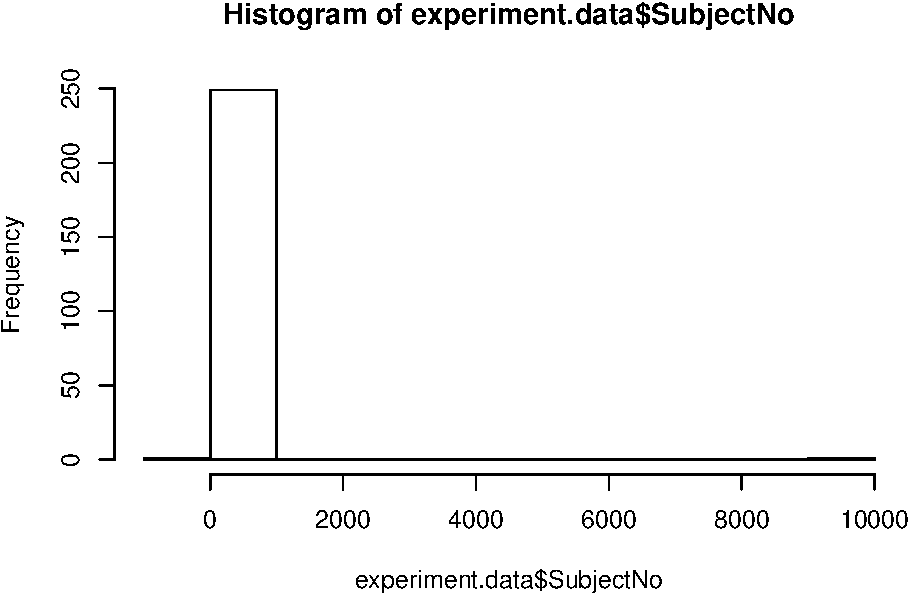
\includegraphics{bookdown-demo_files/figure-latex/unnamed-chunk-34-1.pdf}

Notice that the variable of \texttt{SubjectNo} has negative values and
placeholders! We can use R's indexing function to find these entries.

\begin{Shaded}
\begin{Highlighting}[]
\CommentTok{# Drop those }
\NormalTok{experiment.data <-}\StringTok{ }\NormalTok{experiment.data[experiment.data}\OperatorTok{$}\NormalTok{SubjectNo }\OperatorTok{>}\StringTok{ }\DecValTok{0} \OperatorTok{&}\StringTok{ }\NormalTok{experiment.data}\OperatorTok{$}\NormalTok{SubjectNo }\OperatorTok{<}\StringTok{ }\DecValTok{1000}\NormalTok{,]}
\end{Highlighting}
\end{Shaded}

Note this works because the SubjectNo variable is numeric

\begin{Shaded}
\begin{Highlighting}[]
\KeywordTok{hist}\NormalTok{(experiment.data}\OperatorTok{$}\NormalTok{SubjectNo)}
\end{Highlighting}
\end{Shaded}

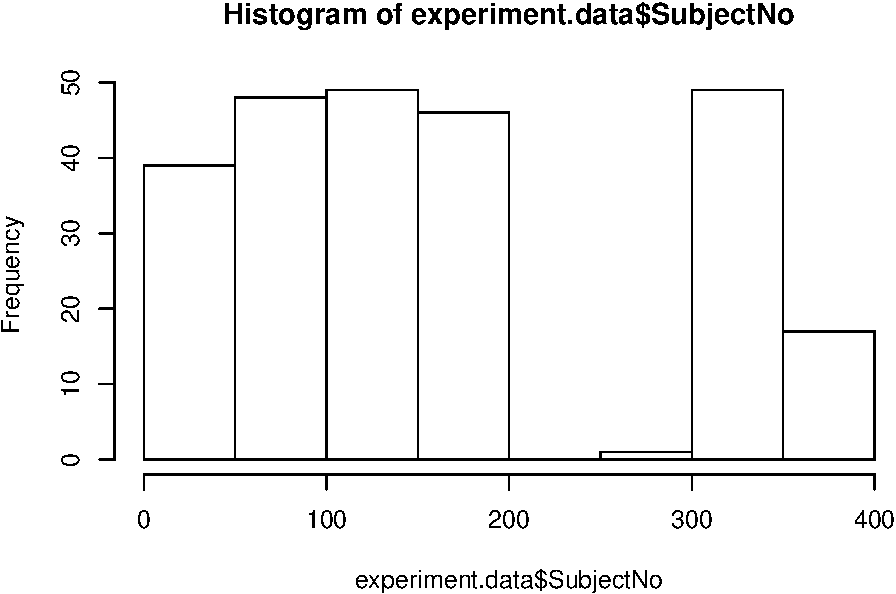
\includegraphics{bookdown-demo_files/figure-latex/unnamed-chunk-36-1.pdf}

\begin{Shaded}
\begin{Highlighting}[]
\KeywordTok{hist}\NormalTok{(item.level.data}\OperatorTok{$}\NormalTok{SubjectNo)}
\end{Highlighting}
\end{Shaded}

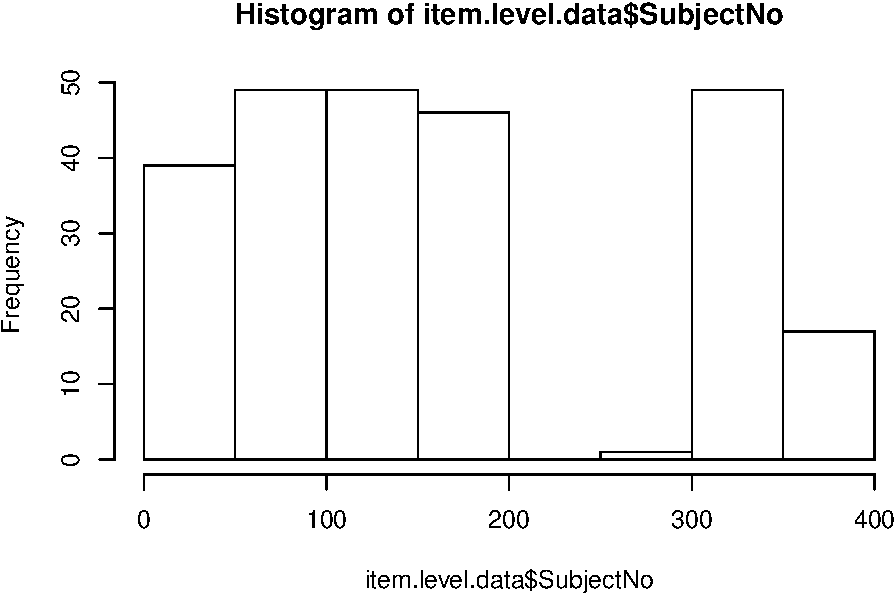
\includegraphics{bookdown-demo_files/figure-latex/unnamed-chunk-36-2.pdf}

Ok, finally we merge our datasets. What we are doing here is called an
``inner join'' Here we will keep all of the ROWS of the dataset in the
middle of the command Note we need to swap over our key to be a
character value.

\begin{Shaded}
\begin{Highlighting}[]
\NormalTok{item.level.data <-}\StringTok{ }\KeywordTok{data.table}\NormalTok{(item.level.data)}
\NormalTok{experiment.data <-}\StringTok{ }\KeywordTok{data.table}\NormalTok{(experiment.data)}

\NormalTok{item.level.data}
\end{Highlighting}
\end{Shaded}

\begin{verbatim}
##      SubjectNo X1 X2 X3 X4 X5 X6 X7 X8 X9 X10 X11 X12 X13 X14 X15 X16 X17
##   1:       100  2  1  5  4  1  5  5  1  4   5   7   1   5   4   3   5   6
##   2:       101  7  5  7  7  3  7  7  4  7   2   6   4   5   5   5   4   6
##   3:       102  4  2  5  4  3  7  4  5  3   4   6   3   2   4   4   5   2
##   4:       103  5  7  7  5  5  7  7  5  7   6   7   2   5   6   5   4   4
##   5:       104  2  1  1  2  1  4  1  5  3   5   6   2   5   6   6   6   1
##  ---                                                                     
## 246:        95  3  2  6  5  3  2  3  3  4   2   6   6   5   6   6   6   3
## 247:        96  5  1  3  5  5  5  6  5  3   5   6   4   2   5   5   5   1
## 248:        97  5  2  4  4  2  3  5  4  2   5   6   4   3   5   5   3   6
## 249:        98  6  2  7  7  6  7  5  3  4   4   7   6   6   6   6   6   7
## 250:        99  5  4  5  5  6  7  7  4  7   2   4   5   2   5   5   4   1
##      X18 X19 X20 X21 X22 X23 X24 X25 X26 X27 X28 X29 X30 X31 X32 X33 X34
##   1:   2   2   2   3   3   3   4   2   2   7   2   5   5   2   1   6   7
##   2:   6   2   1   3   5   1   1   2   3   4   2   4   3   3   2   7   7
##   3:   4   2   1   2   6   4   3   2   2   2   1   2   3   2   2   5   6
##   4:   4   2   1   1   1   3   3   1   1   2   1   5   1   5   4   7   3
##   5:   5   1   1   1   1   1   1   1   3   2   1   1   5   7   5   1   6
##  ---                                                                    
## 246:   6   2   2   1   1   1   1   1   6   6   3   6   6   2   2   2   6
## 247:   6   1   1   1   1   1   1   1   2   6   1   1   6   6   5   2   6
## 248:   5   6   7   3   5   1   5   2   2   5   2   2   4   5   3   5   6
## 249:   7   6   3   7   5   4   4   2   6   6   5   7   7   7   3   6   7
## 250:   5   1   1   2   3   1   1   1   6   5   2   2   3   7   6   6   7
##      X35 X36 X37 X38
##   1:   7   2   4   7
##   2:   7   4   6   7
##   3:   7   5   5   7
##   4:   7   7   7   7
##   5:   6   3   5   7
##  ---                
## 246:   6   5   5   5
## 247:   7   2   5   6
## 248:   5   5   4   5
## 249:   7   5   6   7
## 250:   7   2   6   7
\end{verbatim}

\begin{Shaded}
\begin{Highlighting}[]
\NormalTok{exp.data <-}\StringTok{ }\NormalTok{item.level.data[experiment.data, on=}\StringTok{"SubjectNo"}\NormalTok{]}

\NormalTok{exp.data}
\end{Highlighting}
\end{Shaded}

\begin{verbatim}
##      SubjectNo X1 X2 X3 X4 X5 X6 X7 X8 X9 X10 X11 X12 X13 X14 X15 X16 X17
##   1:        10  2  2  5  6  5  4  7  3  4   6   7   4   6   6   5   4   4
##   2:        11  4  2  4  5  2  5  6  5  4   6   6   3   6   5   5   5   5
##   3:        12  4  2  6  5  2  6  5  2  7   6   6   5   3   6   6   6   6
##   4:        13  5  2  3  7  2  5  5  1  3   4   6   2   4   6   6   5   3
##   5:        14  6  1  6  6  5  6  6  6  6   7   7   6   6   6   6   7   6
##  ---                                                                     
## 245:       363  6  1  5  2  1  7  2  2  1   7   6   3   5   6   6   6   7
## 246:       364  5  3  6  4  3  6  4  4  6   7   5   6   6   6   6   7   7
## 247:       365  3  1  5  2  1  5  5  2  1   6   6   6   5   6   5   6   5
## 248:       366  5  3  5  4  2  5  5  3  3   5   6   5   6   5   6   6   5
## 249:       367  7  5  7  7  7  6  6  7  7   7   7   6   7   6   7   7   5
##      X18 X19 X20 X21 X22 X23 X24 X25 X26 X27 X28 X29 X30 X31 X32 X33 X34
##   1:   5   2   1   5   7   6   5   2   4   6   4   3   4   6   5   7   7
##   2:   6   2   2   2   5   1   3   1   4   5   2   2   2   5   2   5   5
##   3:   5   4   2   4   3   1   5   2   7   6   5   6   6   6   4   5   6
##   4:   6   3   4   6   3   1   6   3   5   5   2   2   2   2   1   6   6
##   5:   6   1   1   1   1   1   1   1   3   1   5   1   2   6   6   7   7
##  ---                                                                    
## 245:   6   7   2   6   5   1   6   2   6   7   7   6   5   2   1   5   6
## 246:   4   7   6   7   5   4   6   3   5   7   6   1   7   6   5   5   6
## 247:   6   6   3   6   3   1   6   2   3   4   2   4   4   2   2   6   6
## 248:   6   5   4   5   3   1   5   3   5   6   4   5   3   4   3   5   6
## 249:   6   7   7   7   7   6   6   3   4   7   6   6   2   6   3   7   7
##      X35 X36 X37 X38 ACTIVE PERCEPTUAL MUSICAL SINGING EMOTIONS GENERAL
##   1:   6   6   6   7     38         47      28      33       39      75
##   2:   6   5   5   6     37         47      16      22       32      67
##   3:   7   2   4   6     39         49      21      40       30      82
##   4:   7   5   5   5     33         42      26      19       34      68
##   5:   6   6   7   2     48         57       7      24       35      60
##  ---                                                                   
## 245:   6   5   7   6     27         52      29      34       35      88
## 246:   6   5   6   7     41         54      38      37       35      96
## 247:   5   3   6   6     25         51      27      21       32      61
## 248:   6   5   7   5     35         50      26      30       34      82
## 249:   7   6   7   7     59         58      43      34       41     103
##           inst Age Gender                             Major
##   1:  clarinet  29 Female               BUSINESS MANAGEMENT
##   2:      bass  22 Female                        psychology
##   3:     Voice  19 Female             COMMUNICATION STUDIES
##   4: saxophone  23   Male            Mechanical Engineering
##   5:      none  23   Male         Interdisciplinary Studies
##  ---                                                       
## 245:     voice  21   Male                        psychology
## 246:     voice  22 Female Psychology and English Literature
## 247:     flute  22 Female                        PSYCHOLOGY
## 248: saxophone  21 Female                        psychology
## 249:   Bassoon  23 Female               Bassoon Performance
##                          Minor SchoolUGorG MuscMajMinor BeginTrain
##   1: HUMAN RESOURCE MANAGEMENT           1            1          9
##   2:                        NA           1            1         10
##   3:               SOCIAL WORK           1            1         10
##   4:                        NA           1            1         11
##   5:              Anthropology           1            1          0
##  ---                                                              
## 245:                                     1            1         13
## 246:                 Sociology           1            1          9
## 247:                 CHEMISTRY           1            1          9
## 248:                   theatre           1            1         12
## 249:                                     2            2          8
##      AbsPitch YearsPrac PeakPrac Live12Mo TheoryTrain FormalYrs NoOfInst
##   1:       no         4        5        9           4         4        1
##   2:       no         1        2       15           0         1        0
##   3:       no         3        1        3           0         3        1
##   4:       no         7        1        2           0         7        2
##   5:       no         0        0       20           0         0        0
##  ---                                                                    
## 245:       no         9        2        3           0         9        1
## 246:       no        14        2       12           2         8        2
## 247:       no         8        1        3           0         9        1
## 248:       no         4        1        9           0         3        2
## 249:       no        12        5       16           6         9        2
##      ActListenMin i.SubjectNo SubRaven RavenB1 RavenB2 RavenB3 RavenTotal
##   1:           60          10       10      10       8      10         28
##   2:           60          11       11       7      10       6         23
##   3:          180          12       12       3       7       7         17
##   4:           45          13       13      10      10      11         31
##   5:          120          14       14       7       8       5         20
##  ---                                                                     
## 245:            6         363      363       6       7       6         19
## 246:          160         364      364       7       8       8         23
## 247:           10         365      365      10      10       9         29
## 248:           35         366      366      10       7       9         26
## 249:          240         367      367       7       6       6         19
##      OspanSub OspanAccError OspanMathError OspanAbsoluteScore
##   1:       10             8             12                 29
##   2:       11             7             12                 20
##   3:       12             7              7                 48
##   4:       13             1              2                 68
##   5:       14             2              2                 33
##  ---                                                         
## 245:      363             2              4                 18
## 246:      364             1              1                 68
## 247:      365             2              8                  4
## 248:      366             4              7                 38
## 249:      367             1              2                 54
##      OspanPartialScore OspanB1 OspanB2 OspanB3 OspanSpeedErrTot SymSub
##   1:                47      21      14      12                4     10
##   2:                41      11      18      12                5     11
##   3:                65      21      23      21                0     12
##   4:                73      25      23      25                1     13
##   5:                50      17      16      17                0     14
##  ---                                                                  
## 245:                28      11       8       9                2    363
## 246:                72      22      25      25                0    364
## 247:                21      10       5       6                6    365
## 248:                58      22      18      18                3    366
## 249:                66      25      22      19                1    367
##      SymAccErrTot SymSpeedErrTot SspanAbsScore SspanPartiaScore SspanB1
##   1:            1              0            10               19       8
##   2:            4              1            15               29      11
##   3:            2              0            21               34      10
##   4:            1              0            27               34      13
##   5:            0              0            15               26       8
##  ---                                                                   
## 245:            0              0             7               21       8
## 246:            0              0            32               38      14
## 247:            0              0            18               28       9
## 248:            2              1            33               40      14
## 249:            2              0            17               28      10
##      SspanB2 SspanB3 SymmErrTot ToneSub ToneAccErrTot ToneMathErrTot
##   1:       4       7          1      10             8              9
##   2:      13       5          5      11             5              5
##   3:      13      11          2      12             8              8
##   4:      10      11          1      13             1              2
##   5:       8      10          0      14             4              5
##  ---                                                                
## 245:       7       6          0     363             7              8
## 246:      13      11          0     364             3              5
## 247:       8      11          0     365             3              4
## 248:      13      13          3     366             6              9
## 249:      10       8          2     367             2              2
##      TspanAbsScore TspanPartScore TspanB1 TspanB2 TspanB3 ToneSpeedErrTot
##   1:             9             36      13       6      17               1
##   2:            21             47      14      19      14               0
##   3:            27             55      17      21      17               0
##   4:            37             63      20      22      21               1
##   5:            10             31       8       9      14               1
##  ---                                                                     
## 245:             6             37      15      13       9               1
## 246:            55             67      22      24      21               2
## 247:            21             38       9      13      16               1
## 248:            32             56      17      16      23               3
## 249:            58             67      23      23      21               0
##      BeatSub BeatTotal BeatAcc MelodicSub MelodicTot MelodicAcc Native
##   1:      10        11    0.61         10          7       0.54      1
##   2:      11        10    0.56         11          7       0.54      1
##   3:      12        14    0.78         12          6       0.46      1
##   4:      13        13    0.72         13         10       0.77      1
##   5:      14        14    0.78         14          5       0.38      1
##  ---                                                                  
## 245:     363        16    0.89        363          7       0.54      1
## 246:     364        11    0.61        364          7       0.54      1
## 247:     365        10    0.56        365         10       0.77      1
## 248:     366         9    0.50        366          9       0.69      1
## 249:     367        12    0.67        367          9       0.69      1
##      Paid jv_NoGMSI jv_nonNative jv_noOspan
##   1:    1         0            0          0
##   2:    1         0            0          0
##   3:    1         0            0          0
##   4:    1         0            0          0
##   5:    1         0            0          0
##  ---                                       
## 245:    2         0            0          0
## 246:    2         0            0          0
## 247:    2         0            0          0
## 248:    2         0            0          0
## 249:    2         0            0          0
\end{verbatim}

Let's reorganize our columns so individual stuff is at the back We could
do this with data.table, but it's a different syntax so let's swap back
Normally you try to stick to minimal switching, but we're just taking a
big tour du R right now and learning to think

\begin{Shaded}
\begin{Highlighting}[]
\NormalTok{exp.data <-}\StringTok{ }\KeywordTok{data.frame}\NormalTok{(exp.data)}
\NormalTok{exp.data <-}\StringTok{ }\NormalTok{exp.data[,}\KeywordTok{c}\NormalTok{(}\DecValTok{1}\NormalTok{,}\DecValTok{40}\OperatorTok{:}\DecValTok{100}\NormalTok{,}\DecValTok{2}\OperatorTok{:}\DecValTok{39}\NormalTok{)]}
\end{Highlighting}
\end{Shaded}

\section{Checking for Univariate
Outliers}\label{checking-for-univariate-outliers}

For this example, let's imagine a univariate outlier is one with a
zscore greater than 3. While we could write a bit of code to look for
this, let's use the pairs.panels() function in the psych pacakge to just
get used to looking at our data The function is not the biggest fan of
huge datasets, so let's index our dataset to only grab what we need. Try
to change the values and look at variables of interest.

\begin{Shaded}
\begin{Highlighting}[]
\KeywordTok{pairs.panels}\NormalTok{(exp.data[,}\DecValTok{2}\OperatorTok{:}\DecValTok{7}\NormalTok{], }\DataTypeTok{lm =} \OtherTok{TRUE}\NormalTok{)}
\end{Highlighting}
\end{Shaded}

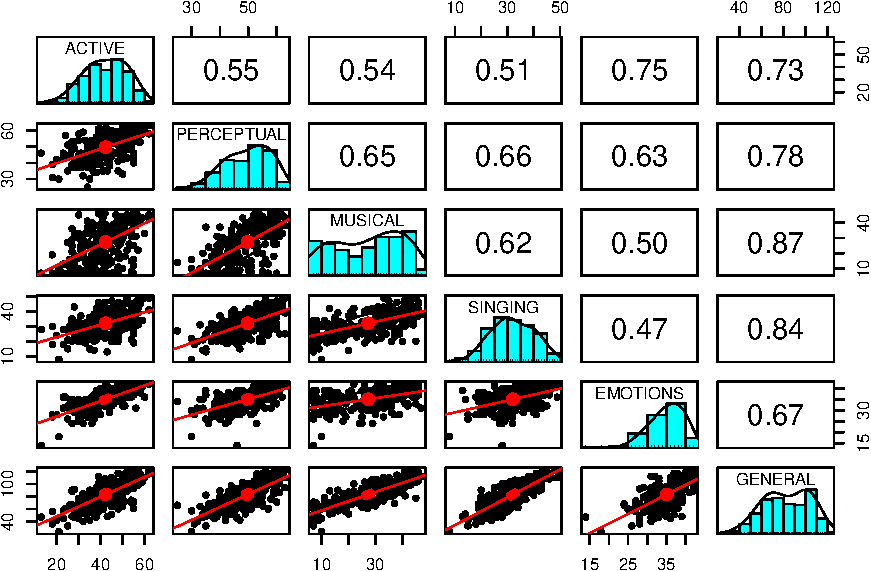
\includegraphics{bookdown-demo_files/figure-latex/unnamed-chunk-39-1.pdf}

But of course we need to look at numbers in terms of their zscores!
Let's first standardize our entire dataset using the apply function Note
we only can do this on numeric values!

The apply function takes 3 argument The first is what you want to
manipulate, the second is if it's rows 1 or columns 2 (remeber this
because it's always rows then columns!), and the function. You can even
write your own (though we'll get to functions later)

\begin{Shaded}
\begin{Highlighting}[]
\NormalTok{gmsi.z.scores <-}\StringTok{ }\KeywordTok{apply}\NormalTok{(exp.data[}\DecValTok{2}\OperatorTok{:}\DecValTok{7}\NormalTok{],}\DecValTok{2}\NormalTok{,scale)}

\NormalTok{exp.data.with.z <-}\StringTok{ }\KeywordTok{cbind}\NormalTok{(exp.data, gmsi.z.scores)}

\CommentTok{#Now we can index this to find values above whatever theshold we want!}

\KeywordTok{table}\NormalTok{(gmsi.z.scores }\OperatorTok{>}\StringTok{ }\DecValTok{2}\NormalTok{)}
\end{Highlighting}
\end{Shaded}

\begin{verbatim}
## 
## FALSE  TRUE 
##  1487     6
\end{verbatim}

\begin{Shaded}
\begin{Highlighting}[]
\NormalTok{gmsi.z.indexer <-}\StringTok{ }\NormalTok{gmsi.z.scores }\OperatorTok{>}\StringTok{ }\DecValTok{2}
\NormalTok{gmsi.z.scores[gmsi.z.indexer] }\CommentTok{# See what they are, find them , decide to get rid of}
\end{Highlighting}
\end{Shaded}

\begin{verbatim}
## [1]       NA 2.053441 2.053441 2.142711 2.016431 2.142711 2.142711
\end{verbatim}

\subsection{Checking for Multivariate
Outliers}\label{checking-for-multivariate-outliers}

A bit tricker, I leanred how to do this off a blog post.

\begin{Shaded}
\begin{Highlighting}[]
\NormalTok{gmsi.responses <-}\StringTok{ }\NormalTok{exp.data[,}\KeywordTok{c}\NormalTok{(}\DecValTok{63}\OperatorTok{:}\DecValTok{100}\NormalTok{)]}

\NormalTok{mahal <-}\StringTok{ }\KeywordTok{mahalanobis}\NormalTok{(gmsi.responses,}
                     \KeywordTok{colMeans}\NormalTok{(gmsi.responses, }\DataTypeTok{na.rm =} \OtherTok{TRUE}\NormalTok{), }
                     \KeywordTok{cov}\NormalTok{(gmsi.responses, }
                         \DataTypeTok{use =} \StringTok{"pairwise.complete.obs"}\NormalTok{))                    ## Create Distance Measures}

\NormalTok{cutoff <-}\StringTok{ }\KeywordTok{qchisq}\NormalTok{(.}\DecValTok{999}\NormalTok{, }\KeywordTok{ncol}\NormalTok{(gmsi.responses))                                ## Create cutoff object .001 signifiance and DF = obs}
\KeywordTok{summary}\NormalTok{(mahal }\OperatorTok{<}\StringTok{ }\NormalTok{cutoff)                                                     ## 11 Subjects greater than 70 cutoff }
\end{Highlighting}
\end{Shaded}

\begin{verbatim}
##    Mode   FALSE    TRUE 
## logical      11     238
\end{verbatim}

\begin{Shaded}
\begin{Highlighting}[]
\CommentTok{# Add On Variables }
\NormalTok{exp.data}\OperatorTok{$}\NormalTok{mahal <-}\StringTok{ }\NormalTok{mahal}
\NormalTok{exp.data <-}\StringTok{ }\KeywordTok{data.table}\NormalTok{(exp.data) }\CommentTok{# To use easier indexer, needs data.table }
\NormalTok{exp.data[exp.data}\OperatorTok{$}\NormalTok{mahal }\OperatorTok{<}\StringTok{ }\NormalTok{cutoff]}
\end{Highlighting}
\end{Shaded}

\begin{verbatim}
##      SubjectNo ACTIVE PERCEPTUAL MUSICAL SINGING EMOTIONS GENERAL
##   1:        10     38         47      28      33       39      75
##   2:        11     37         47      16      22       32      67
##   3:        12     39         49      21      40       30      82
##   4:        13     33         42      26      19       34      68
##   5:        15     47         55       8      24       36      65
##  ---                                                             
## 234:       363     27         52      29      34       35      88
## 235:       364     41         54      38      37       35      96
## 236:       365     25         51      27      21       32      61
## 237:       366     35         50      26      30       34      82
## 238:       367     59         58      43      34       41     103
##           inst Age Gender                             Major
##   1:  clarinet  29 Female               BUSINESS MANAGEMENT
##   2:      bass  22 Female                        psychology
##   3:     Voice  19 Female             COMMUNICATION STUDIES
##   4: saxophone  23   Male            Mechanical Engineering
##   5:     piano  19 Female                         marketing
##  ---                                                       
## 234:     voice  21   Male                        psychology
## 235:     voice  22 Female Psychology and English Literature
## 236:     flute  22 Female                        PSYCHOLOGY
## 237: saxophone  21 Female                        psychology
## 238:   Bassoon  23 Female               Bassoon Performance
##                          Minor SchoolUGorG MuscMajMinor BeginTrain
##   1: HUMAN RESOURCE MANAGEMENT           1            1          9
##   2:                        NA           1            1         10
##   3:               SOCIAL WORK           1            1         10
##   4:                        NA           1            1         11
##   5:                        NA           1            1          0
##  ---                                                              
## 234:                                     1            1         13
## 235:                 Sociology           1            1          9
## 236:                 CHEMISTRY           1            1          9
## 237:                   theatre           1            1         12
## 238:                                     2            2          8
##      AbsPitch YearsPrac PeakPrac Live12Mo TheoryTrain FormalYrs NoOfInst
##   1:       no         4        5        9           4         4        1
##   2:       no         1        2       15           0         1        0
##   3:       no         3        1        3           0         3        1
##   4:       no         7        1        2           0         7        2
##   5:       no         0        0        9           0         0        0
##  ---                                                                    
## 234:       no         9        2        3           0         9        1
## 235:       no        14        2       12           2         8        2
## 236:       no         8        1        3           0         9        1
## 237:       no         4        1        9           0         3        2
## 238:       no        12        5       16           6         9        2
##      ActListenMin i.SubjectNo SubRaven RavenB1 RavenB2 RavenB3 RavenTotal
##   1:           60          10       10      10       8      10         28
##   2:           60          11       11       7      10       6         23
##   3:          180          12       12       3       7       7         17
##   4:           45          13       13      10      10      11         31
##   5:           60          15       15       6      10       6         22
##  ---                                                                     
## 234:            6         363      363       6       7       6         19
## 235:          160         364      364       7       8       8         23
## 236:           10         365      365      10      10       9         29
## 237:           35         366      366      10       7       9         26
## 238:          240         367      367       7       6       6         19
##      OspanSub OspanAccError OspanMathError OspanAbsoluteScore
##   1:       10             8             12                 29
##   2:       11             7             12                 20
##   3:       12             7              7                 48
##   4:       13             1              2                 68
##   5:       15            12             15                 20
##  ---                                                         
## 234:      363             2              4                 18
## 235:      364             1              1                 68
## 236:      365             2              8                  4
## 237:      366             4              7                 38
## 238:      367             1              2                 54
##      OspanPartialScore OspanB1 OspanB2 OspanB3 OspanSpeedErrTot SymSub
##   1:                47      21      14      12                4     10
##   2:                41      11      18      12                5     11
##   3:                65      21      23      21                0     12
##   4:                73      25      23      25                1     13
##   5:                44      14      17      13                3     15
##  ---                                                                  
## 234:                28      11       8       9                2    363
## 235:                72      22      25      25                0    364
## 236:                21      10       5       6                6    365
## 237:                58      22      18      18                3    366
## 238:                66      25      22      19                1    367
##      SymAccErrTot SymSpeedErrTot SspanAbsScore SspanPartiaScore SspanB1
##   1:            1              0            10               19       8
##   2:            4              1            15               29      11
##   3:            2              0            21               34      10
##   4:            1              0            27               34      13
##   5:            4              1             9               25       9
##  ---                                                                   
## 234:            0              0             7               21       8
## 235:            0              0            32               38      14
## 236:            0              0            18               28       9
## 237:            2              1            33               40      14
## 238:            2              0            17               28      10
##      SspanB2 SspanB3 SymmErrTot ToneSub ToneAccErrTot ToneMathErrTot
##   1:       4       7          1      10             8              9
##   2:      13       5          5      11             5              5
##   3:      13      11          2      12             8              8
##   4:      10      11          1      13             1              2
##   5:      10       6          5      15             7             10
##  ---                                                                
## 234:       7       6          0     363             7              8
## 235:      13      11          0     364             3              5
## 236:       8      11          0     365             3              4
## 237:      13      13          3     366             6              9
## 238:      10       8          2     367             2              2
##      TspanAbsScore TspanPartScore TspanB1 TspanB2 TspanB3 ToneSpeedErrTot
##   1:             9             36      13       6      17               1
##   2:            21             47      14      19      14               0
##   3:            27             55      17      21      17               0
##   4:            37             63      20      22      21               1
##   5:             4             34       9      12      13               3
##  ---                                                                     
## 234:             6             37      15      13       9               1
## 235:            55             67      22      24      21               2
## 236:            21             38       9      13      16               1
## 237:            32             56      17      16      23               3
## 238:            58             67      23      23      21               0
##      BeatSub BeatTotal BeatAcc MelodicSub MelodicTot MelodicAcc X1 X2 X3
##   1:      10        11    0.61         10          7       0.54  2  2  5
##   2:      11        10    0.56         11          7       0.54  4  2  4
##   3:      12        14    0.78         12          6       0.46  4  2  6
##   4:      13        13    0.72         13         10       0.77  5  2  3
##   5:      15        10    0.56         15          5       0.38  7  2  5
##  ---                                                                    
## 234:     363        16    0.89        363          7       0.54  6  1  5
## 235:     364        11    0.61        364          7       0.54  5  3  6
## 236:     365        10    0.56        365         10       0.77  3  1  5
## 237:     366         9    0.50        366          9       0.69  5  3  5
## 238:     367        12    0.67        367          9       0.69  7  5  7
##      X4 X5 X6 X7 X8 X9 X10 X11 X12 X13 X14 X15 X16 X17 X18 X19 X20 X21 X22
##   1:  6  5  4  7  3  4   6   7   4   6   6   5   4   4   5   2   1   5   7
##   2:  5  2  5  6  5  4   6   6   3   6   5   5   5   5   6   2   2   2   5
##   3:  5  2  6  5  2  7   6   6   5   3   6   6   6   6   5   4   2   4   3
##   4:  7  2  5  5  1  3   4   6   2   4   6   6   5   3   6   3   4   6   3
##   5:  7  5  7  7  3  4   7   7   3   5   6   7   7   7   6   2   1   1   1
##  ---                                                                      
## 234:  2  1  7  2  2  1   7   6   3   5   6   6   6   7   6   7   2   6   5
## 235:  4  3  6  4  4  6   7   5   6   6   6   6   7   7   4   7   6   7   5
## 236:  2  1  5  5  2  1   6   6   6   5   6   5   6   5   6   6   3   6   3
## 237:  4  2  5  5  3  3   5   6   5   6   5   6   6   5   6   5   4   5   3
## 238:  7  7  6  6  7  7   7   7   6   7   6   7   7   5   6   7   7   7   7
##      X23 X24 X25 X26 X27 X28 X29 X30 X31 X32 X33 X34 X35 X36 X37 X38
##   1:   6   5   2   4   6   4   3   4   6   5   7   7   6   6   6   7
##   2:   1   3   1   4   5   2   2   2   5   2   5   5   6   5   5   6
##   3:   1   5   2   7   6   5   6   6   6   4   5   6   7   2   4   6
##   4:   1   6   3   5   5   2   2   2   2   1   6   6   7   5   5   5
##   5:   1   1   1   1   7   3   1   1   6   5   5   7   7   5   5   7
##  ---                                                                
## 234:   1   6   2   6   7   7   6   5   2   1   5   6   6   5   7   6
## 235:   4   6   3   5   7   6   1   7   6   5   5   6   6   5   6   7
## 236:   1   6   2   3   4   2   4   4   2   2   6   6   5   3   6   6
## 237:   1   5   3   5   6   4   5   3   4   3   5   6   6   5   7   5
## 238:   6   6   3   4   7   6   6   2   6   3   7   7   7   6   7   7
##         mahal
##   1: 51.21448
##   2: 25.99414
##   3: 29.78012
##   4: 49.15429
##   5: 43.12685
##  ---         
## 234: 58.63224
## 235: 35.67417
## 236: 34.53619
## 237: 17.72908
## 238: 20.60059
\end{verbatim}

\subsection{Checking for Skew and
Kurtosis}\label{checking-for-skew-and-kurtosis}

\begin{Shaded}
\begin{Highlighting}[]
\KeywordTok{apply}\NormalTok{(gmsi.responses, }\DecValTok{2}\NormalTok{, skew)}
\end{Highlighting}
\end{Shaded}

\begin{verbatim}
##           X1           X2           X3           X4           X5 
## -0.751959493  0.403676499 -1.078653410 -0.813983811  0.067614732 
##           X6           X7           X8           X9          X10 
## -1.133338356 -1.056888584  0.003114209  0.174997119 -1.251450954 
##          X11          X12          X13          X14          X15 
## -1.209870193 -0.643154118 -1.046476716 -1.023134965 -1.512836098 
##          X16          X17          X18          X19          X20 
## -0.918246164 -0.549121749 -0.931025766 -0.607086647 -0.009797227 
##          X21          X22          X23          X24          X25 
## -0.324554196 -0.342355019  0.502388714 -0.404073175  1.103530636 
##          X26          X27          X28          X29          X30 
## -0.419299836 -1.204955610 -0.411695100 -0.409111747 -0.082358311 
##          X31          X32          X33          X34          X35 
## -1.037773224  0.068284056 -1.083784471 -1.825310783 -1.693280548 
##          X36          X37          X38 
## -0.651012271 -1.218176414 -2.364635137
\end{verbatim}

\begin{Shaded}
\begin{Highlighting}[]
\KeywordTok{apply}\NormalTok{(gmsi.responses, }\DecValTok{2}\NormalTok{ , kurtosi)}
\end{Highlighting}
\end{Shaded}

\begin{verbatim}
##          X1          X2          X3          X4          X5          X6 
## -0.27214952 -0.83327603  1.14629947  0.02931285 -1.30675305  0.83305054 
##          X7          X8          X9         X10         X11         X12 
##  1.36849018 -0.92937707 -0.69656989  1.58298149  2.00805464 -0.58320443 
##         X13         X14         X15         X16         X17         X18 
##  0.49964877  1.30350514  2.47139233  0.56622834 -0.89787441  0.80425156 
##         X19         X20         X21         X22         X23         X24 
## -1.18236897 -1.67596746 -1.49414255 -1.24558633 -1.41680710 -1.30953622 
##         X25         X26         X27         X28         X29         X30 
##  0.42141756 -0.69749482  0.73800105 -1.08494701 -0.90943305 -1.31818613 
##         X31         X32         X33         X34         X35         X36 
##  0.86327735 -1.00536155  0.46640336  4.08373503  4.90078751 -0.09764595 
##         X37         X38 
##  2.04104393  9.60389299
\end{verbatim}

\subsection{Exporting Data}\label{exporting-data}

It's best practice to separate your cleaning and your analysis into
separate scripts. Export the dataset you have into a new csv file into a
directory that would make sense to someone who has never seen your
project before.

\begin{Shaded}
\begin{Highlighting}[]
\KeywordTok{write.csv}\NormalTok{(exp.data,}\StringTok{"datasets/My_Experiment_Data.csv"}\NormalTok{)}
\end{Highlighting}
\end{Shaded}

\chapter{Epistemology of Statistics}\label{epistemology-of-statistics}

We describe our methods in this chapter.

\chapter{Descriptive Statistics, z Scores, Central
Limit}\label{descriptive-statistics-z-scores-central-limit}

\section{Descriptive Statistics and the Normal
Distribution}\label{descriptive-statistics-and-the-normal-distribution}

\subsection{Organizing Data}\label{organizing-data}

Descriptive statistics are traditionally used to summarize data from
observed samples. Most often, sample data are organized into
distributions of information based on ascending scores. For example, we
might have a table with some SAT-Verbal scores from a few different
students. Before going on to think about this, also take note that the
shape of this data (though very minimal) is in the tidy format.
According to Hadley Wickham on the
\href{https://cran.r-project.org/web/packages/tidyr/vignettes/tidy-data.html}{tidyr
CRAN page} for data to be tidy it must have the following properties:

\begin{enumerate}
\def\labelenumi{\arabic{enumi}.}
\tightlist
\item
  Each variable forms a column.
\item
  Each observation forms a row.
\item
  Each type of observational unit forms a table.
\end{enumerate}

This isn't very important right now, but once you get to more complex
designs, it will be good to have had thought about this before.

\begin{Shaded}
\begin{Highlighting}[]
\NormalTok{student <-}\StringTok{ }\KeywordTok{c}\NormalTok{(}\DecValTok{1}\NormalTok{,}\DecValTok{2}\NormalTok{,}\DecValTok{3}\NormalTok{,}\DecValTok{4}\NormalTok{,}\DecValTok{5}\NormalTok{,}\DecValTok{6}\NormalTok{)}
\NormalTok{SAT <-}\StringTok{ }\KeywordTok{c}\NormalTok{(}\DecValTok{480}\NormalTok{,}\DecValTok{530}\NormalTok{,}\DecValTok{560}\NormalTok{,}\DecValTok{650}\NormalTok{,}\DecValTok{720}\NormalTok{,}\DecValTok{760}\NormalTok{)}
\NormalTok{satData <-}\StringTok{ }\KeywordTok{data.frame}\NormalTok{(student,SAT)}
\NormalTok{satData}
\end{Highlighting}
\end{Shaded}

\begin{verbatim}
##   student SAT
## 1       1 480
## 2       2 530
## 3       3 560
## 4       4 650
## 5       5 720
## 6       6 760
\end{verbatim}

\subsection{Shape of Data}\label{shape-of-data}

When visualized, data can take on a variety of shapes. Below are a few
of the shapes you might come across when analyzing data.

The first, and probably least likely distribution you will find is the
\textbf{uniform} or \textbf{rectangular distribution}. We can create
this plot and the others by using the
\href{https://en.wikibooks.org/wiki/R_Programming/Probability_Distributions\#Uniform_distribution}{distribution
functions} from R's functionality. In each case we are going to take
1,000 samples from 0 to 1. We'll plot everything using \texttt{ggplot2}
so we can also get used to using it for our packages.

\begin{Shaded}
\begin{Highlighting}[]
\KeywordTok{library}\NormalTok{(ggplot2)}
\KeywordTok{set.seed}\NormalTok{(}\DecValTok{666}\NormalTok{)}
\NormalTok{uniformData <-}\StringTok{ }\KeywordTok{runif}\NormalTok{(}\DataTypeTok{n=}\DecValTok{1000}\NormalTok{, }\DataTypeTok{min=}\DecValTok{0}\NormalTok{, }\DataTypeTok{max=}\DecValTok{100}\NormalTok{)}
\NormalTok{distributions <-}\StringTok{ }\KeywordTok{data.frame}\NormalTok{(uniformData)}

\CommentTok{# Make variable to remove ggplot elements }
\NormalTok{cleanUpPlots <-}\StringTok{  }\KeywordTok{theme}\NormalTok{(}\DataTypeTok{axis.title.x=}\KeywordTok{element_blank}\NormalTok{(),}
                  \DataTypeTok{axis.text.x=}\KeywordTok{element_blank}\NormalTok{(),}
                  \DataTypeTok{axis.ticks.x=}\KeywordTok{element_blank}\NormalTok{(),}
                  \DataTypeTok{axis.text.y=}\KeywordTok{element_blank}\NormalTok{(),}
                  \DataTypeTok{axis.ticks.y=}\KeywordTok{element_blank}\NormalTok{())}

\KeywordTok{ggplot}\NormalTok{(distributions, }\KeywordTok{aes}\NormalTok{(distributions}\OperatorTok{$}\NormalTok{uniformData)) }\OperatorTok{+}\StringTok{ }
\StringTok{  }\KeywordTok{geom_histogram}\NormalTok{(}\DataTypeTok{binwidth =} \DecValTok{5}\NormalTok{) }\OperatorTok{+}
\StringTok{  }\KeywordTok{labs}\NormalTok{(}\DataTypeTok{x =} \StringTok{"Independent Variable"}\NormalTok{, }\DataTypeTok{y =} \StringTok{"Frequency"}\NormalTok{, }\DataTypeTok{title =} \StringTok{"Uniform Distribution"}\NormalTok{) }\OperatorTok{+}\StringTok{ }\NormalTok{cleanUpPlots}
\end{Highlighting}
\end{Shaded}

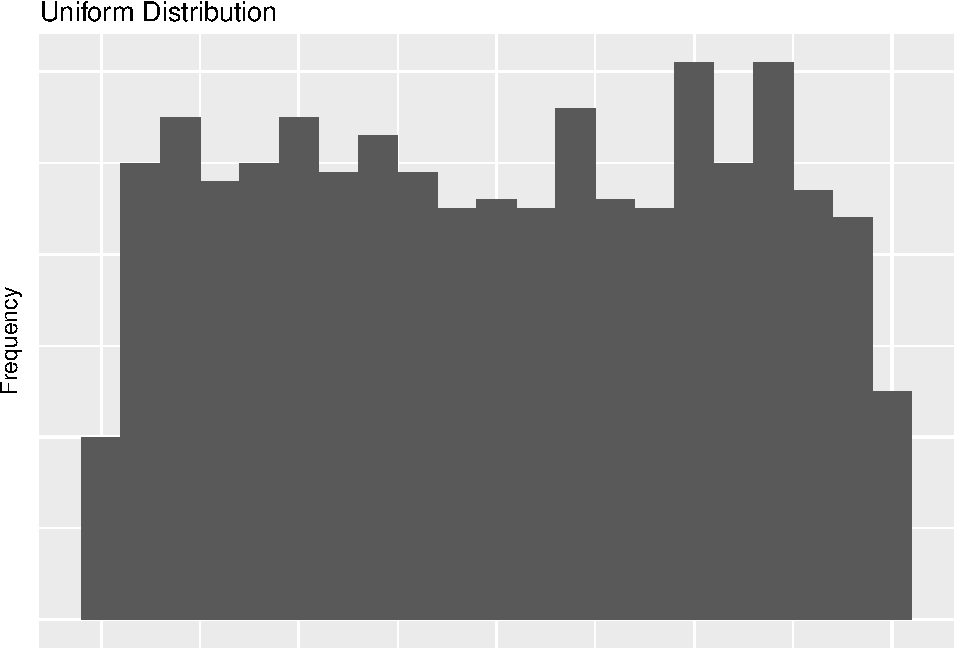
\includegraphics{bookdown-demo_files/figure-latex/unnamed-chunk-45-1.pdf}

Try to run the above code with different arguments in the
\texttt{binwidth} argument. You'll notice that the way you plot the data
will actually represent it differntly.

We can also have \textbf{positively skewed} and \textbf{negatively
skewed} distributions. If a distribution is skewed, it usually means
that the \textbf{mode} does not equal the \textbf{mean}. We're going to
approximate both of these with another one of R's probability functions.

\begin{Shaded}
\begin{Highlighting}[]
\NormalTok{positiveSkewData <-}\StringTok{ }\KeywordTok{rchisq}\NormalTok{(}\DecValTok{1000}\NormalTok{,}\DecValTok{6}\NormalTok{) }\CommentTok{# Chi Square distributions are positively skewed}
\NormalTok{negativeSkewData <-}\StringTok{ }\OperatorTok{-}\StringTok{ }\NormalTok{positiveSkewData }\CommentTok{# Flip it!}
\NormalTok{distributions <-}\StringTok{ }\KeywordTok{data.frame}\NormalTok{(uniformData, positiveSkewData, negativeSkewData)}
\KeywordTok{ggplot}\NormalTok{(distributions, }\KeywordTok{aes}\NormalTok{(distributions}\OperatorTok{$}\NormalTok{positiveSkewData)) }\OperatorTok{+}\StringTok{ }
\StringTok{  }\KeywordTok{geom_histogram}\NormalTok{(}\DataTypeTok{binwidth =} \DecValTok{1}\NormalTok{) }\OperatorTok{+}
\StringTok{  }\KeywordTok{labs}\NormalTok{(}\DataTypeTok{x =} \StringTok{"Independent Variable"}\NormalTok{, }\DataTypeTok{y =} \StringTok{"Frequency"}\NormalTok{, }\DataTypeTok{title =} \StringTok{"Positive Skew Distribution"}\NormalTok{) }\OperatorTok{+}\StringTok{    }\NormalTok{cleanUpPlots}
\end{Highlighting}
\end{Shaded}

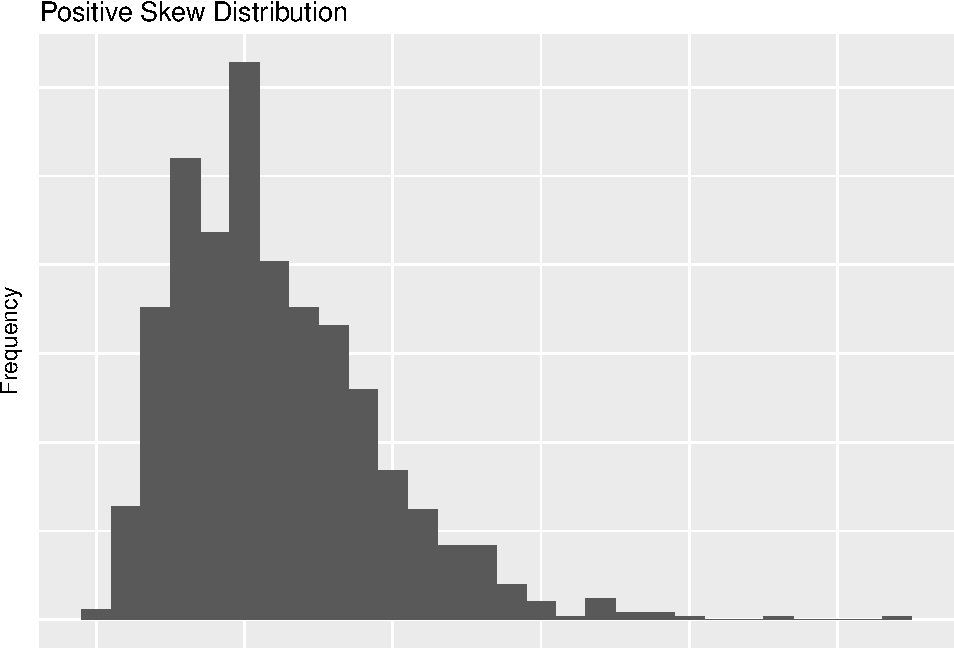
\includegraphics{bookdown-demo_files/figure-latex/unnamed-chunk-46-1.pdf}

\begin{Shaded}
\begin{Highlighting}[]
\KeywordTok{ggplot}\NormalTok{(distributions, }\KeywordTok{aes}\NormalTok{(distributions}\OperatorTok{$}\NormalTok{negativeSkewData)) }\OperatorTok{+}\StringTok{ }
\StringTok{  }\KeywordTok{geom_histogram}\NormalTok{(}\DataTypeTok{binwidth =} \DecValTok{1}\NormalTok{) }\OperatorTok{+}
\StringTok{  }\KeywordTok{labs}\NormalTok{(}\DataTypeTok{x =} \StringTok{"Independent Variable"}\NormalTok{, }\DataTypeTok{y =} \StringTok{"Frequency"}\NormalTok{, }\DataTypeTok{title =} \StringTok{"Negative Skew Distribution"}\NormalTok{) }\OperatorTok{+}\StringTok{   }\NormalTok{cleanUpPlots}
\end{Highlighting}
\end{Shaded}

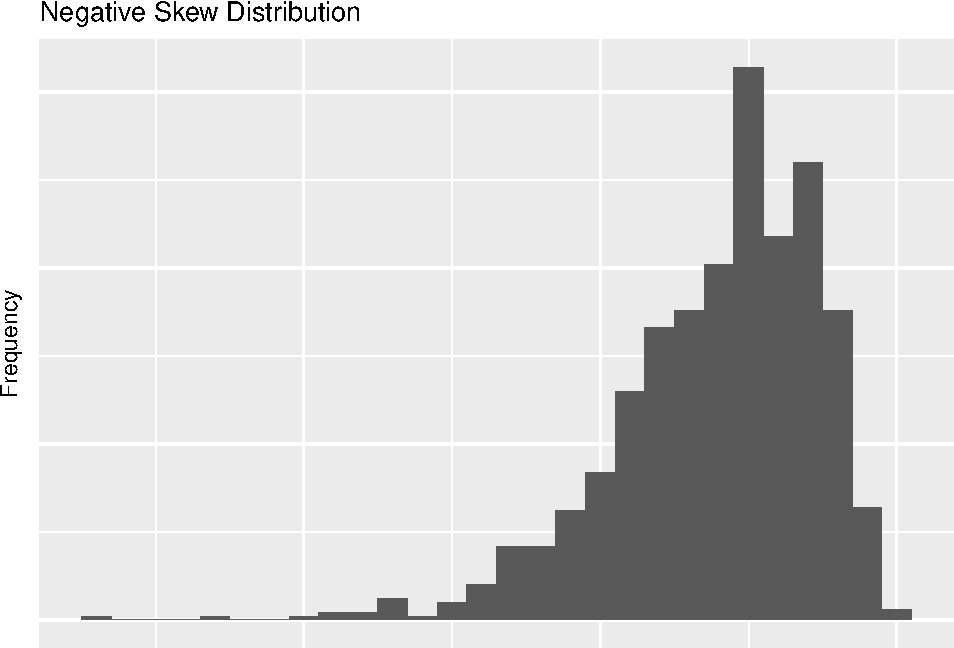
\includegraphics{bookdown-demo_files/figure-latex/unnamed-chunk-46-2.pdf}

The most important distribution in the world of Frequentist statistics
is a \textbf{normal distribution}. A normal distribution is defined by
THIS HERE.

\begin{Shaded}
\begin{Highlighting}[]
\NormalTok{normalData <-}\StringTok{ }\KeywordTok{rnorm}\NormalTok{(}\DataTypeTok{n =} \DecValTok{1000}\NormalTok{,}\DataTypeTok{mean =} \DecValTok{0}\NormalTok{,}\DataTypeTok{sd =} \DecValTok{2}\NormalTok{) }\CommentTok{# Flip it!}
\NormalTok{distributions <-}\StringTok{ }\KeywordTok{data.frame}\NormalTok{(uniformData, positiveSkewData, negativeSkewData, normalData)}
\KeywordTok{ggplot}\NormalTok{(distributions, }\KeywordTok{aes}\NormalTok{(distributions}\OperatorTok{$}\NormalTok{normalData)) }\OperatorTok{+}\StringTok{ }
\StringTok{  }\KeywordTok{geom_histogram}\NormalTok{(}\DataTypeTok{binwidth =} \DecValTok{1}\NormalTok{) }\OperatorTok{+}
\StringTok{  }\KeywordTok{labs}\NormalTok{(}\DataTypeTok{x =} \StringTok{"Independent Variable"}\NormalTok{, }\DataTypeTok{y =} \StringTok{"Frequency"}\NormalTok{, }\DataTypeTok{title =} \StringTok{"Normal Distribution"}\NormalTok{) }\OperatorTok{+}\StringTok{    }\NormalTok{cleanUpPlots}
\end{Highlighting}
\end{Shaded}

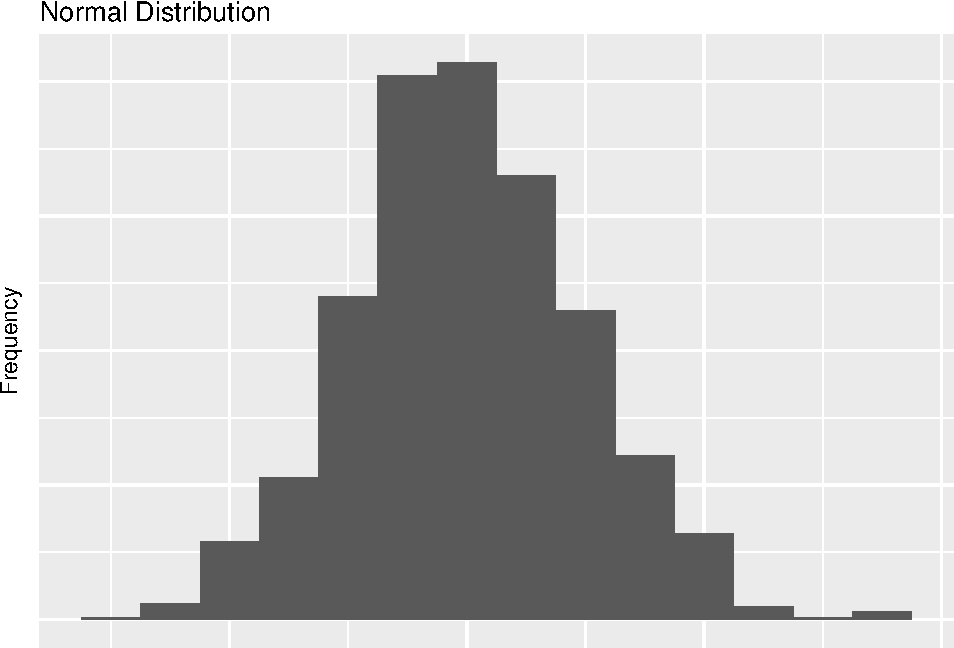
\includegraphics{bookdown-demo_files/figure-latex/unnamed-chunk-47-1.pdf}

And the lastly we can have both \textbf{leptokurtic} and
\textbf{platykurtic} distributions.

\begin{Shaded}
\begin{Highlighting}[]
\NormalTok{leptoData <-}\StringTok{ }\KeywordTok{rnorm}\NormalTok{(}\DataTypeTok{n =} \DecValTok{1000}\NormalTok{,}\DataTypeTok{mean =} \DecValTok{0}\NormalTok{,}\DataTypeTok{sd =} \DecValTok{2}\NormalTok{) }
\NormalTok{platyData <-}\StringTok{ }\KeywordTok{rnorm}\NormalTok{(}\DataTypeTok{n =} \DecValTok{1000}\NormalTok{,}\DataTypeTok{mean =} \DecValTok{0}\NormalTok{,}\DataTypeTok{sd =} \DecValTok{2}\NormalTok{)}
\NormalTok{distributions <-}\StringTok{ }\KeywordTok{data.frame}\NormalTok{(uniformData, positiveSkewData, negativeSkewData, normalData,leptoData, platyData)}
\KeywordTok{ggplot}\NormalTok{(distributions, }\KeywordTok{aes}\NormalTok{(distributions}\OperatorTok{$}\NormalTok{leptoData)) }\OperatorTok{+}\StringTok{ }
\StringTok{  }\KeywordTok{geom_histogram}\NormalTok{(}\DataTypeTok{binwidth =} \DecValTok{1}\NormalTok{) }\OperatorTok{+}
\StringTok{  }\KeywordTok{labs}\NormalTok{(}\DataTypeTok{x =} \StringTok{"Independent Variable"}\NormalTok{, }\DataTypeTok{y =} \StringTok{"Frequency"}\NormalTok{, }\DataTypeTok{title =} \StringTok{"Leptokurtic Distribution, FIX ME"}\NormalTok{) }\OperatorTok{+}\StringTok{    }\NormalTok{cleanUpPlots}
\end{Highlighting}
\end{Shaded}

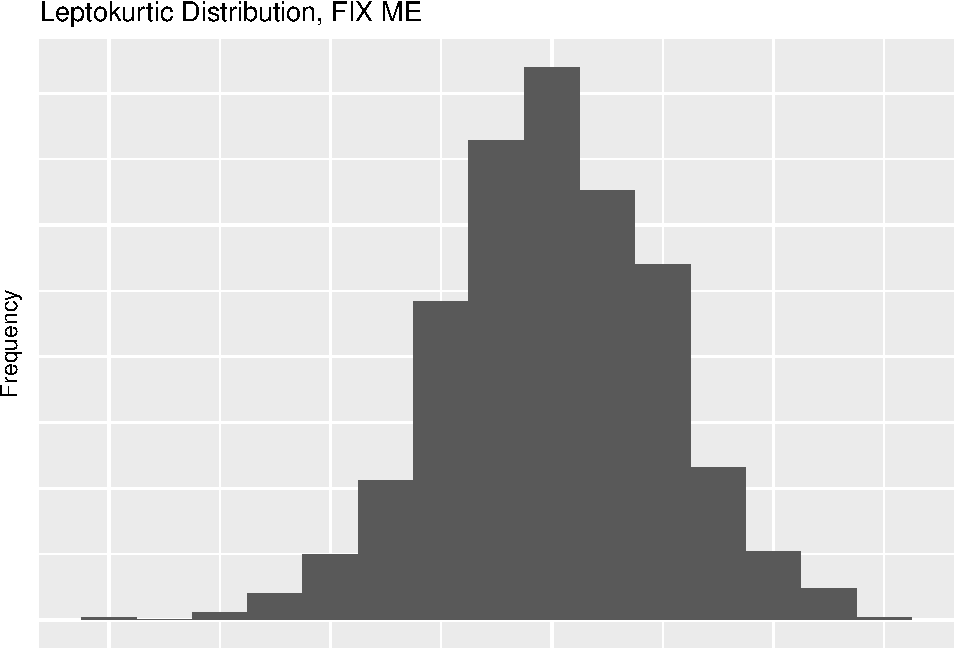
\includegraphics{bookdown-demo_files/figure-latex/unnamed-chunk-48-1.pdf}

\begin{Shaded}
\begin{Highlighting}[]
\KeywordTok{ggplot}\NormalTok{(distributions, }\KeywordTok{aes}\NormalTok{(distributions}\OperatorTok{$}\NormalTok{platyData)) }\OperatorTok{+}\StringTok{ }
\StringTok{  }\KeywordTok{geom_histogram}\NormalTok{(}\DataTypeTok{binwidth =} \DecValTok{1}\NormalTok{) }\OperatorTok{+}
\StringTok{  }\KeywordTok{labs}\NormalTok{(}\DataTypeTok{x =} \StringTok{"Independent Variable"}\NormalTok{, }\DataTypeTok{y =} \StringTok{"Frequency"}\NormalTok{, }\DataTypeTok{title =} \StringTok{"Platykurtic Distribution, FIX ME"}\NormalTok{) }\OperatorTok{+}\StringTok{    }\NormalTok{cleanUpPlots}
\end{Highlighting}
\end{Shaded}

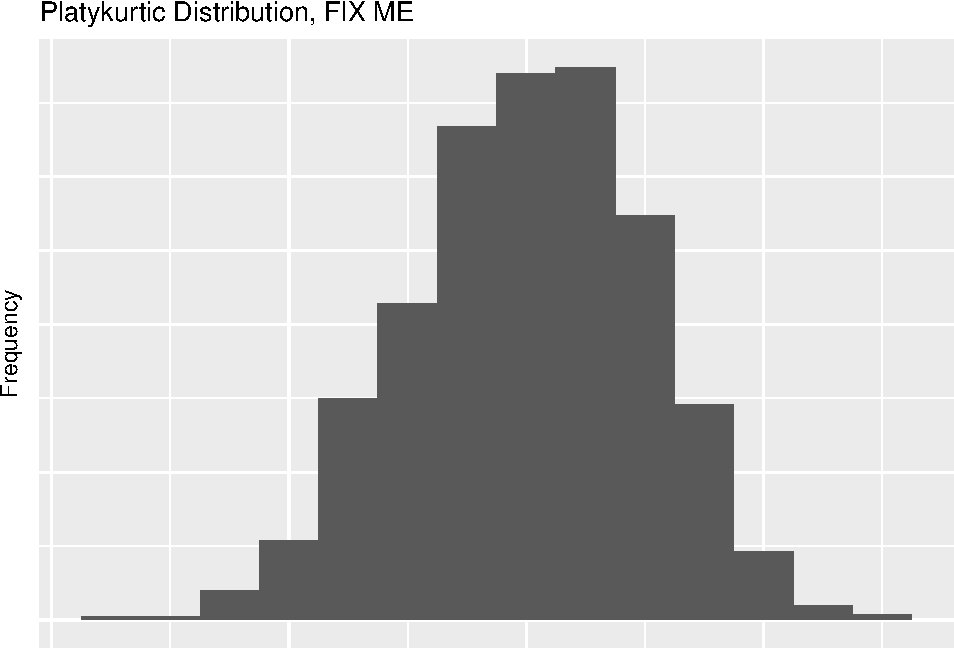
\includegraphics{bookdown-demo_files/figure-latex/unnamed-chunk-48-2.pdf}

Generally measurses of \textbf{central tendency} are used to
characterize the most typical score in a distribution.

For example we could calculate the \textbf{mean} or the \textbf{median}
of our SAT data. The mean is calculated by adding up all our numbers,
designated with the Greek letter Sigma \(\Sigma\) then dividing by the
amount of numbers we added up, or \(n\). As an equation it would look
like this.

\[\bar{X} = \frac{(\Sigma\ x_i)}{n}\]

Take a second to talk yourself through that so later you will start to
feel more comfortable with more complex equational notation. Some people
find it helpful to just try to say the equation in plain English. In
this case it would be the mean, or \(\bar{x}\) is defined as or equal to
what happens when you add up \(\Sigma\) every single value \(x\) that
you have going up to \(i\), then divide all those numbers by the amount
of numbers you have, or \(n\).

The median is defined by finding the middle number. If there is a tie
because we have an even set of numbers, we take the mean of the middle
two numbers.

We can do both of these in R as well. Below we can either type in the
numbers as you would with a calculator, or use a function in R. Notice
that each step when its typed out is saved into an object. By starting
to think this way, it will pave the way for writing more elegant code
later on.

\begin{Shaded}
\begin{Highlighting}[]
\CommentTok{# Typing it out }
\NormalTok{our.data <-}\StringTok{ }\KeywordTok{c}\NormalTok{(}\DecValTok{480} \OperatorTok{+}\StringTok{ }\DecValTok{530} \OperatorTok{+}\StringTok{ }\DecValTok{560} \OperatorTok{+}\StringTok{ }\DecValTok{650} \OperatorTok{+}\StringTok{ }\DecValTok{720} \OperatorTok{+}\StringTok{ }\DecValTok{760}\NormalTok{)}
\NormalTok{how.many <-}\StringTok{ }\KeywordTok{length}\NormalTok{(our.data)}
\NormalTok{our.data}\OperatorTok{/}\NormalTok{how.many}
\end{Highlighting}
\end{Shaded}

\begin{verbatim}
## [1] 3700
\end{verbatim}

\begin{Shaded}
\begin{Highlighting}[]
\CommentTok{# Inbuilt functions}
\KeywordTok{mean}\NormalTok{(satData}\OperatorTok{$}\NormalTok{SAT)}
\end{Highlighting}
\end{Shaded}

\begin{verbatim}
## [1] 616.6667
\end{verbatim}

\begin{Shaded}
\begin{Highlighting}[]
\KeywordTok{median}\NormalTok{(satData}\OperatorTok{$}\NormalTok{SAT)}
\end{Highlighting}
\end{Shaded}

\begin{verbatim}
## [1] 605
\end{verbatim}

Notice here that for adding up the means by hand I could have done what
programmers call hard coded the equation in. That would have looked like
this.

\begin{Shaded}
\begin{Highlighting}[]
\NormalTok{our.answer <-}\StringTok{ }\KeywordTok{c}\NormalTok{(}\DecValTok{480} \OperatorTok{+}\StringTok{ }\DecValTok{530} \OperatorTok{+}\StringTok{ }\DecValTok{560} \OperatorTok{+}\StringTok{ }\DecValTok{650} \OperatorTok{+}\StringTok{ }\DecValTok{720} \OperatorTok{+}\StringTok{ }\DecValTok{760}\NormalTok{) }\OperatorTok{/}\StringTok{ }\DecValTok{6}
\NormalTok{our.answer}
\end{Highlighting}
\end{Shaded}

\begin{verbatim}
## [1] 616.6667
\end{verbatim}

The problem with this, is that every time you get a new SAT score you
have to both enter the score and update how many scores you are dividing
by. Whenever you see a chance to take a shortcut like this, do it! It
will save you tons of time in the future.

\subsection{Important Considerations for Central
Tendency}\label{important-considerations-for-central-tendency}

There are three big considerations to think about when choosing numbers
to represent your data.

\begin{enumerate}
\def\labelenumi{\arabic{enumi}.}
\tightlist
\item
  The mode is the most variable from sample to sample; the mean is the
  least variable
\item
  The mean is the most sensitive to extreme scores; e.g., skewed
  distributions
\item
  The mean is the most frequently used measure because \emph{The sum of
  the deviations around the mean is 0 }The sum of the squared deviations
  is the smallest around the mean, rather than the mode or median; this
  is known as the least squares principle
\end{enumerate}

\subsection{Measures of Variability}\label{measures-of-variability}

The \textbf{range} is simply the largest score minus the smallest score.
It is the crudest measure of variability. In our dataset we would
calculate it with the following code.

\begin{Shaded}
\begin{Highlighting}[]
\DecValTok{760} \OperatorTok{-}\StringTok{ }\DecValTok{480}
\end{Highlighting}
\end{Shaded}

\begin{verbatim}
## [1] 280
\end{verbatim}

\begin{Shaded}
\begin{Highlighting}[]
\CommentTok{# OR}
\KeywordTok{range}\NormalTok{(satData}\OperatorTok{$}\NormalTok{SAT)}
\end{Highlighting}
\end{Shaded}

\begin{verbatim}
## [1] 480 760
\end{verbatim}

\begin{Shaded}
\begin{Highlighting}[]
\KeywordTok{max}\NormalTok{(satData}\OperatorTok{$}\NormalTok{SAT) }\OperatorTok{-}\StringTok{ }\KeywordTok{min}\NormalTok{(satData}\OperatorTok{$}\NormalTok{SAT)}
\end{Highlighting}
\end{Shaded}

\begin{verbatim}
## [1] 280
\end{verbatim}

The interquartile rangerepresents the spread between the score at the
75th and 25th percentiles. Boxplots are often used to graphically
represent inner 50\% of the scores.

\begin{Shaded}
\begin{Highlighting}[]
\NormalTok{y <-}\StringTok{ }\NormalTok{satData}\OperatorTok{$}\NormalTok{SAT}
\NormalTok{boxplot.example <-}\StringTok{ }\KeywordTok{data.frame}\NormalTok{(}
          \DataTypeTok{x =} \DecValTok{1}\NormalTok{,}
          \DataTypeTok{y0 =} \KeywordTok{min}\NormalTok{(y),}
          \DataTypeTok{y25 =} \KeywordTok{quantile}\NormalTok{(y, }\FloatTok{0.25}\NormalTok{),}
          \DataTypeTok{y50 =} \KeywordTok{median}\NormalTok{(y),}
          \DataTypeTok{y75 =} \KeywordTok{quantile}\NormalTok{(y, }\FloatTok{0.75}\NormalTok{),}
          \DataTypeTok{y100 =} \KeywordTok{max}\NormalTok{(y)}
\NormalTok{)}

\KeywordTok{ggplot}\NormalTok{(boxplot.example, }\KeywordTok{aes}\NormalTok{(x)) }\OperatorTok{+}
\StringTok{    }\KeywordTok{labs}\NormalTok{(}\DataTypeTok{title =} \StringTok{"Example of Boxplot"}\NormalTok{) }\OperatorTok{+}\StringTok{ }\KeywordTok{geom_boxplot}\NormalTok{(}\KeywordTok{aes}\NormalTok{(}\DataTypeTok{ymin =}\NormalTok{ y0, }\DataTypeTok{lower =}\NormalTok{ y25, }\DataTypeTok{middle =}\NormalTok{ y50, }\DataTypeTok{upper =}\NormalTok{ y75, }\DataTypeTok{ymax =}\NormalTok{ y100),}
    \DataTypeTok{stat =} \StringTok{"identity"}\NormalTok{)}
\end{Highlighting}
\end{Shaded}

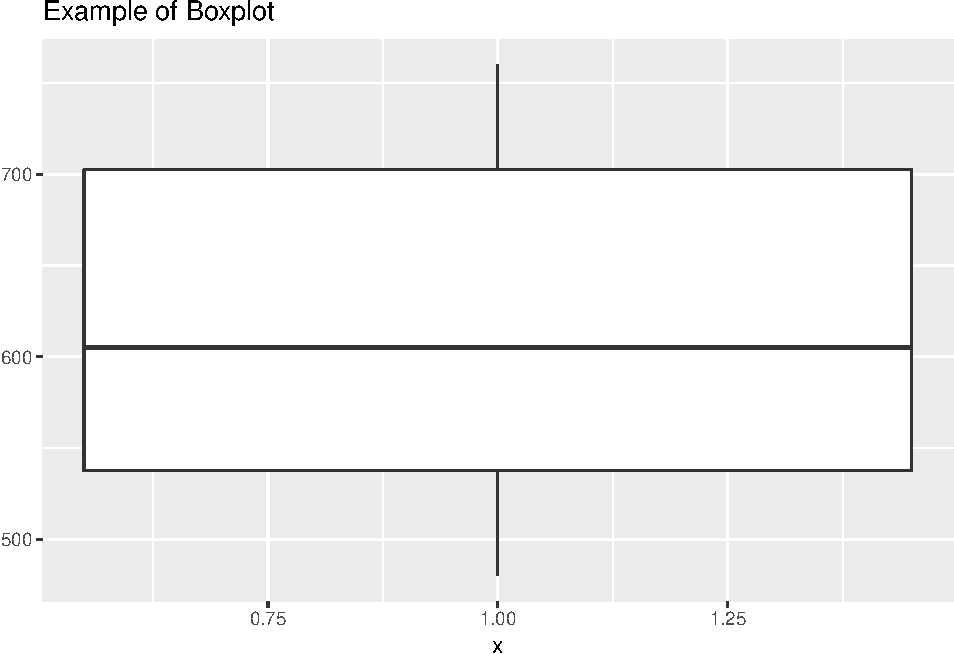
\includegraphics{bookdown-demo_files/figure-latex/unnamed-chunk-52-1.pdf}

The \textbf{variance} is essentially the averaged squared deviation
around the mean. Now there is a very important distinction that we will
get to a bit later on, but that is the difference between a
\textbf{population} value or \(\sigma^2\) and a \textbf{sample} variance
or \(s^2\). In order to do frequentist statistics, we need to assume
that there is some sort of True value that the group we are measuring
has and it is a fundamental property of the group! For more on this see
CHAPTER 3 and the work of Zoltan Dienes. Somewhere, maybe written on a
golden plate in heaven is the actual value of the average weight of a
labrador retriever. The problem is we will never have access to that
information so we need to estimate it by using a sample. The logic is
that if we can truly draw in a random way from our entire population, in
this case labrador retrievers, the central limit theroum will give us a
good approximation of what that True value will be. Since we want to be
clear about when we are talking about the Platonic, True value and the
actual sample we collected, we use different Greek notation. The
\(\sigma^2\) refers to the Platonic value and the \(\sigma^2\) is the
sample. They are defined as follows:

\[\sigma^2 = \frac{\Sigma(X_i - \mu)^2}{N}\]

\[s^2 = \frac{\Sigma(X_i - \mu)^2}{n-1}\]

Note here that each of these formulas needs a mean. In the population
equation that is defined as \(\mu\) and in samples we used \(\bar{X}\).

In our case with the SAT scores, we are wanting to know the True value
of the SAT scores of whatever population our six students are theorized
to come from. To do the calulations below we need to know the mean which
we calcualted above to be 616.67.

Now since these scores are to serve as a represntive \textbf{sample} in
hopes of getting at the true population value we need to use the formula
reflecting the \textbf{sample variance} or \(s^2\).

\[s^2 = \frac{(480-616.7)^2 + . . . + (760 - 616.676)^2}{6-1}\]

Doing this by hand we get an \(s^2\) value of 12346.67. Or running it in
R, we would use.

\begin{Shaded}
\begin{Highlighting}[]
\KeywordTok{var}\NormalTok{(satData}\OperatorTok{$}\NormalTok{SAT)}
\end{Highlighting}
\end{Shaded}

\begin{verbatim}
## [1] 12346.67
\end{verbatim}

The \textbf{standard deviation} is the square root of the variance of
the sample.

\[s = \sqrt\frac{\Sigma(X_i - \mu)^2}{n-1}\]

And since we know \(s^2\) from above, we can shorten this to

\[s = \sqrt{s^2} = \sqrt{12345.67} = 111.12\]

Or run it in R and get

\begin{Shaded}
\begin{Highlighting}[]
\KeywordTok{sd}\NormalTok{(satData}\OperatorTok{$}\NormalTok{SAT)}
\end{Highlighting}
\end{Shaded}

\begin{verbatim}
## [1] 111.1156
\end{verbatim}

\textbf{Standard scores} represent the distance of raw scores form their
mean in standard deviation units.

\[z = \frac{x_i - \bar{X}}{s}\]

So if we needed to find the \(z\) score or standardized score for
someone who got a 560 on their SAT we could compute the following.

\[z_{560} = \frac{560 - 616.67}{111.12} = -0.51\]

Interpreted in-context, this would mean that if you scored a 560 on the
SAT, based on our sample (which we think helps us get at the True
popuation value), you would be scoring about less than 1 standard
deviation (the unit of z) below the average.

\subsection{Properties of z Scores}\label{properties-of-z-scores}

Z scores are defined by having having three separte properties:

\begin{enumerate}
\def\labelenumi{\arabic{enumi}.}
\tightlist
\item
  The standardized distribution preserves the shape of the original raw
  score distribution
\item
  The mean of the standardized distribution is always 0
\item
  The variance \& standard deviation are always 1
\end{enumerate}

Many of the variables in behavioral sciences are distributed normally.
In addition, the basis for parametric inferential statistics is based on
the normal distribution.

The normal distribution is unimodal, symmetrical, bell shaped, with a
maximum height at the mean. The normal distribution is continuous and
additionallythe normal distribution is asymptotic to the X axis---it
never actually touches the X axis and theoretically goes on to infinity.

The normal distribution is really a family of distributions defined by
all possible combinations of means \(\mu\) and standard deviations
\(\sigma\). We can use the standardized normal distribution to find
areas of probability under the curve.

With a normal distribution, there is always a fixed area under the curve
which we take the reflect the probability of getting a score when
sampling from a population.

For example if we go 1 z unit (1 SD) away from the mean we find 34\% of
the total area of the curve there. If you then extend that out to the
negative side, you then encapsulate 68\% of the distribution. This would
translate to a scenario where if you were to get a score at random from
the distribution, 68\% of the time you would get a score between 1 and
-1 SD units from your mean.

This process can be extended as seen in the figure below.

\begin{figure}
\centering
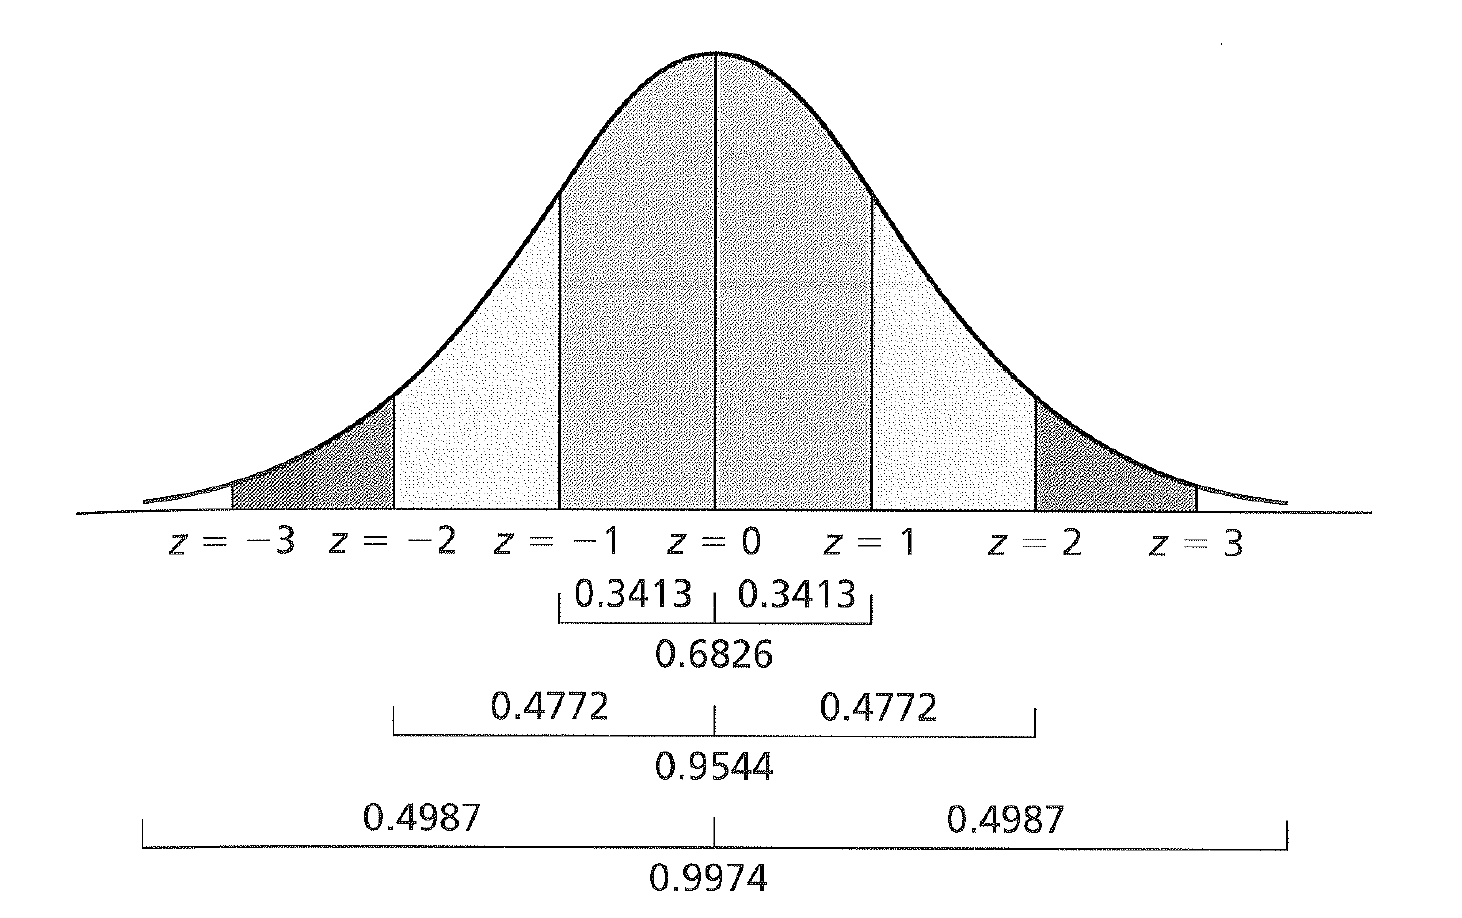
\includegraphics{img/hickszscores1.png}
\caption{z Scores and Areas Under the Curve}
\end{figure}

We could also calculate the area between two z scores as shown here.
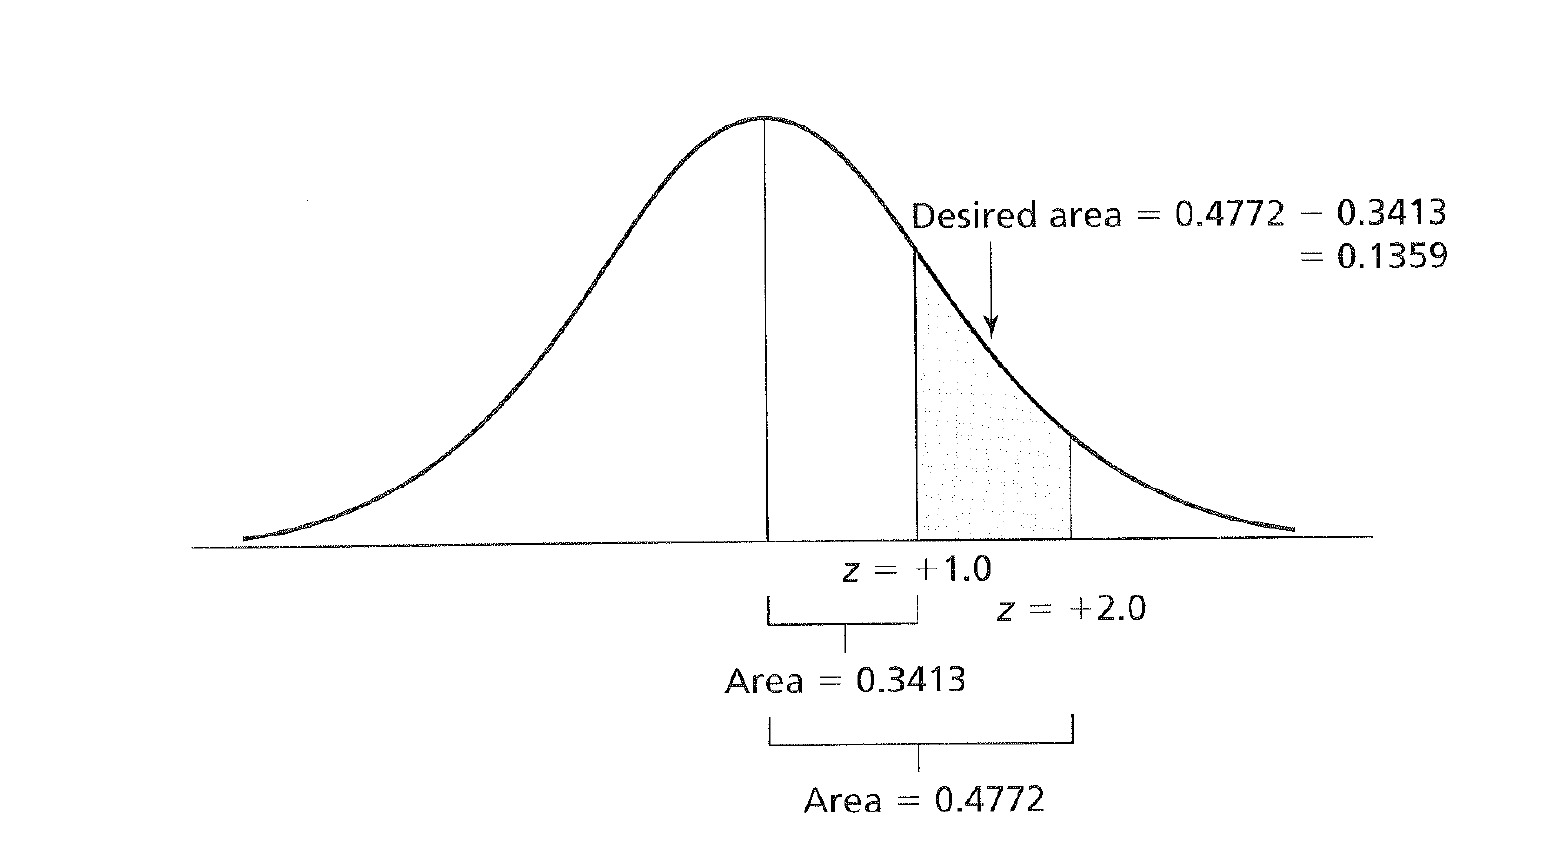
\includegraphics{img/hickszscores2.png}

And we could also look at how much area under the distribution exists
beyond two standard deviations beyond the mean.

\begin{figure}
\centering
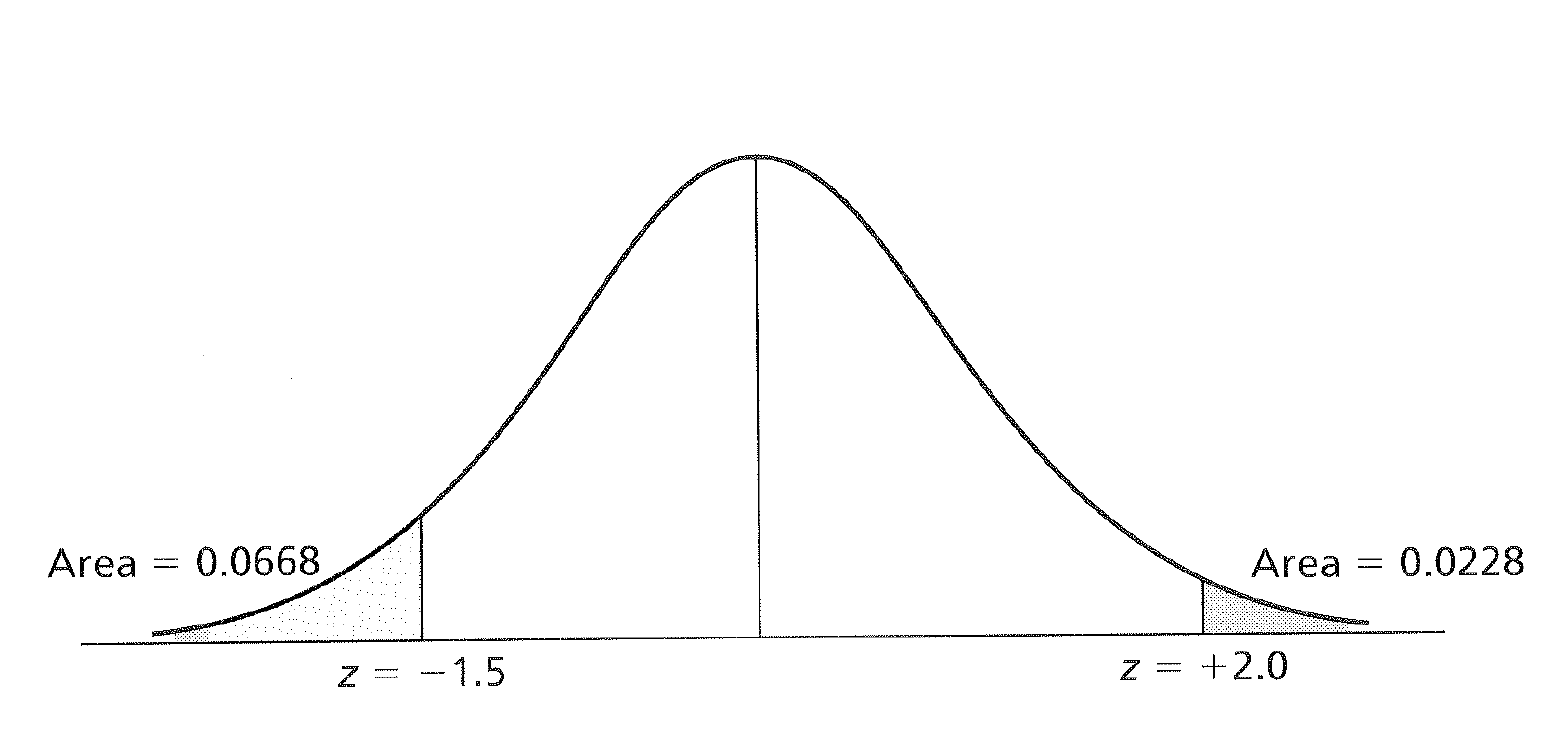
\includegraphics{img/hickszscores3.png}
\caption{z Scores and Areas Under the Curve}
\end{figure}

Or we could pick any z score values and find the area under the mean!

\begin{figure}
\centering
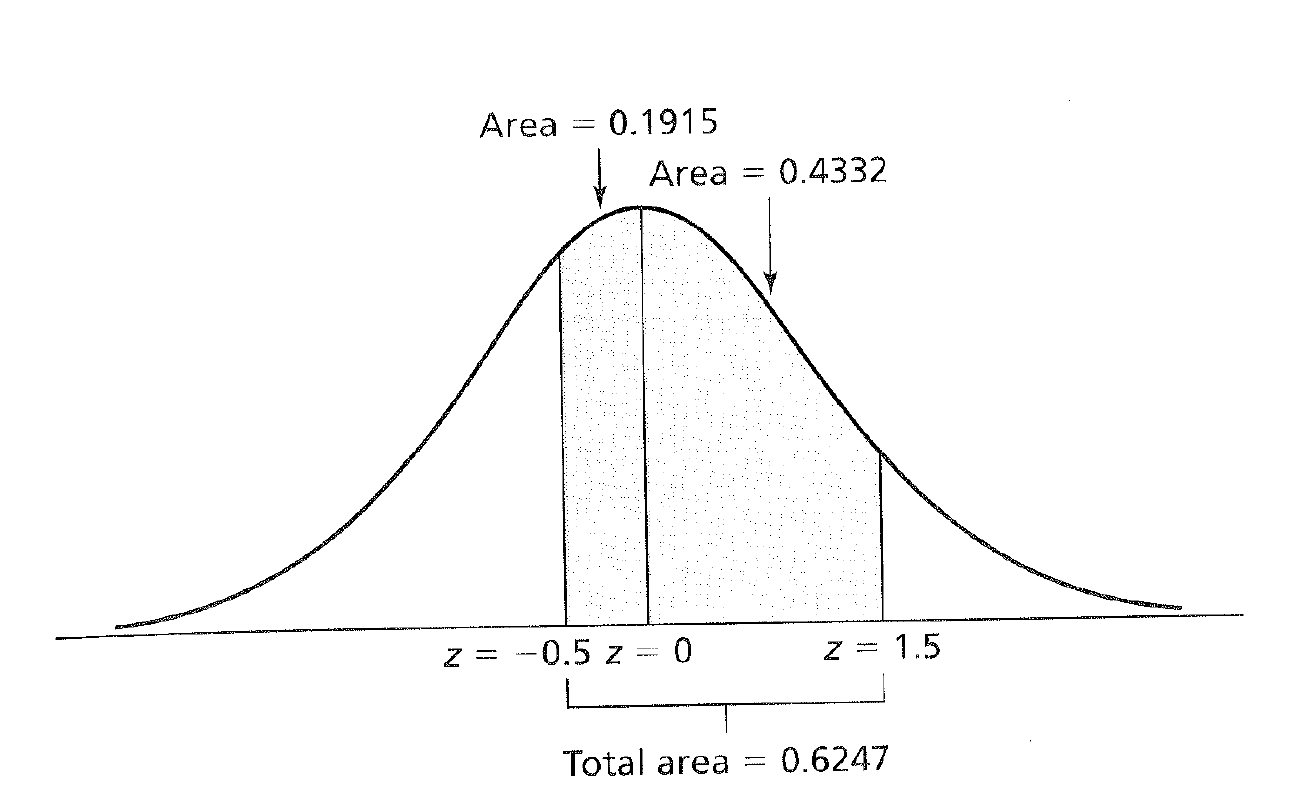
\includegraphics{img/hickszscores4.png}
\caption{z Scores and Areas Under the Curve}
\end{figure}

\section{Practice}\label{practice}

We can now start to put this to use. Here are some past homework
examples.

During tryouts, a sample of ballet dancers were rated on their athletic
ability andoverall knowledge of the art. Below are the ratings for each
dancer (a score above 75 percent means that the dancer will join the
troupe

83, 98, 45, 69, 52, 94, 82, 74, 71, 83, 62, 85, 90, 97, 61, 74, 74, 88

Let's put them into R so we can use answer a few questions about our
data.

\begin{Shaded}
\begin{Highlighting}[]
\NormalTok{ballet <-}\StringTok{ }\KeywordTok{c}\NormalTok{(}\DecValTok{83}\NormalTok{, }\DecValTok{98}\NormalTok{, }\DecValTok{45}\NormalTok{, }\DecValTok{69}\NormalTok{, }\DecValTok{52}\NormalTok{, }\DecValTok{94}\NormalTok{, }\DecValTok{82}\NormalTok{, }\DecValTok{74}\NormalTok{, }\DecValTok{71}\NormalTok{, }\DecValTok{83}\NormalTok{, }\DecValTok{62}\NormalTok{, }\DecValTok{85}\NormalTok{, }\DecValTok{90}\NormalTok{, }\DecValTok{97}\NormalTok{, }\DecValTok{61}\NormalTok{, }\DecValTok{74}\NormalTok{, }\DecValTok{74}\NormalTok{, }\DecValTok{88}\NormalTok{)}
\end{Highlighting}
\end{Shaded}

What is the median percentage?

\begin{Shaded}
\begin{Highlighting}[]
\KeywordTok{median}\NormalTok{(ballet)}
\end{Highlighting}
\end{Shaded}

\begin{verbatim}
## [1] 78
\end{verbatim}

What is the mean percentage?

\begin{Shaded}
\begin{Highlighting}[]
\KeywordTok{mean}\NormalTok{(ballet)}
\end{Highlighting}
\end{Shaded}

\begin{verbatim}
## [1] 76.77778
\end{verbatim}

What is the standard deviation for the sample (assume we don't know any
population characteristics)?

\begin{Shaded}
\begin{Highlighting}[]
\KeywordTok{sd}\NormalTok{(ballet)}
\end{Highlighting}
\end{Shaded}

\begin{verbatim}
## [1] 15.02373
\end{verbatim}

Demonstrate the least squares principle by showing that the sum of
squares (SS) around the mean is smaller than the sum of squares around
the median (remember to show your work for each).

\begin{Shaded}
\begin{Highlighting}[]
\NormalTok{ballet_mean <-}\StringTok{ }\KeywordTok{mean}\NormalTok{(ballet)}
\NormalTok{ballet_median <-}\StringTok{ }\KeywordTok{median}\NormalTok{(ballet)}
\NormalTok{ballet_sd <-}\StringTok{ }\KeywordTok{sd}\NormalTok{(ballet)}
\end{Highlighting}
\end{Shaded}

Now we can use these values to do our math!

\begin{Shaded}
\begin{Highlighting}[]
\KeywordTok{sum}\NormalTok{((ballet }\OperatorTok{-}\StringTok{ }\NormalTok{ballet_mean)}\OperatorTok{^}\DecValTok{2}\NormalTok{)}
\end{Highlighting}
\end{Shaded}

\begin{verbatim}
## [1] 3837.111
\end{verbatim}

\begin{Shaded}
\begin{Highlighting}[]
\KeywordTok{sum}\NormalTok{((ballet }\OperatorTok{-}\StringTok{ }\NormalTok{ballet_median)}\OperatorTok{^}\DecValTok{2}\NormalTok{)}
\end{Highlighting}
\end{Shaded}

\begin{verbatim}
## [1] 3864
\end{verbatim}

\begin{Shaded}
\begin{Highlighting}[]
\CommentTok{# Then having R do the final work for us}
\KeywordTok{sum}\NormalTok{((ballet }\OperatorTok{-}\StringTok{ }\NormalTok{ballet_mean)}\OperatorTok{^}\DecValTok{2}\NormalTok{) }\OperatorTok{>}\StringTok{ }\KeywordTok{sum}\NormalTok{((ballet }\OperatorTok{-}\StringTok{ }\NormalTok{ballet_median)}\OperatorTok{^}\DecValTok{2}\NormalTok{)}
\end{Highlighting}
\end{Shaded}

\begin{verbatim}
## [1] FALSE
\end{verbatim}

What are the standardized (z) scores for the raw scores 73, 99, and 66?
If you know the population mean and the sd, you can calulate a z score
using the formula \[z =  \frac{x_i - \bar{X}}{s}\]

Or in our case

\begin{Shaded}
\begin{Highlighting}[]
\NormalTok{(}\DecValTok{73} \OperatorTok{-}\StringTok{ }\NormalTok{ballet_mean)}\OperatorTok{/}\StringTok{ }\NormalTok{ballet_sd}
\end{Highlighting}
\end{Shaded}

\begin{verbatim}
## [1] -0.2514541
\end{verbatim}

\begin{Shaded}
\begin{Highlighting}[]
\NormalTok{(}\DecValTok{99} \OperatorTok{-}\StringTok{ }\NormalTok{ballet_mean)}\OperatorTok{/}\StringTok{ }\NormalTok{ballet_sd}
\end{Highlighting}
\end{Shaded}

\begin{verbatim}
## [1] 1.479142
\end{verbatim}

\begin{Shaded}
\begin{Highlighting}[]
\NormalTok{(}\DecValTok{66} \OperatorTok{-}\StringTok{ }\NormalTok{ballet_mean)}\OperatorTok{/}\StringTok{ }\NormalTok{ballet_sd}
\end{Highlighting}
\end{Shaded}

\begin{verbatim}
## [1] -0.7173837
\end{verbatim}

What proportion of scores exceeds a raw score of 73?

\begin{Shaded}
\begin{Highlighting}[]
\KeywordTok{pnorm}\NormalTok{(}\DataTypeTok{q =} \DecValTok{73}\NormalTok{, }\DataTypeTok{mean =}\NormalTok{ ballet_mean, }\DataTypeTok{sd =}\NormalTok{  ballet_sd)}
\end{Highlighting}
\end{Shaded}

\begin{verbatim}
## [1] 0.4007315
\end{verbatim}

To get the other side of the probability we can remember that we can
treat the line above as an object!

\begin{Shaded}
\begin{Highlighting}[]
\DecValTok{1} \OperatorTok{-}\StringTok{ }\KeywordTok{pnorm}\NormalTok{(}\DataTypeTok{q =} \DecValTok{73}\NormalTok{, }\DataTypeTok{mean =}\NormalTok{ ballet_mean, }\DataTypeTok{sd =}\NormalTok{  ballet_sd)}
\end{Highlighting}
\end{Shaded}

\begin{verbatim}
## [1] 0.5992685
\end{verbatim}

What proportion of scores lies between the raw scores of 75 and 100?
Let's be clever for this one and just put the two equations together for
this one. Or if you want, you could save them into objects.

\begin{Shaded}
\begin{Highlighting}[]
\KeywordTok{pnorm}\NormalTok{(}\DataTypeTok{q =} \DecValTok{100}\NormalTok{, }\DataTypeTok{mean =}\NormalTok{ ballet_mean, }\DataTypeTok{sd =}\NormalTok{  ballet_sd) }\OperatorTok{-}\StringTok{ }\KeywordTok{pnorm}\NormalTok{(}\DataTypeTok{q =} \DecValTok{75}\NormalTok{, }\DataTypeTok{mean =}\NormalTok{ ballet_mean, }\DataTypeTok{sd =}\NormalTok{  ballet_sd)}
\end{Highlighting}
\end{Shaded}

\begin{verbatim}
## [1] 0.4860093
\end{verbatim}

\begin{Shaded}
\begin{Highlighting}[]
\KeywordTok{pnorm}\NormalTok{(}\DataTypeTok{q =} \DecValTok{76}\NormalTok{, }\DataTypeTok{mean =}\NormalTok{ ballet_mean, }\DataTypeTok{sd =}\NormalTok{  ballet_sd)}
\end{Highlighting}
\end{Shaded}

\begin{verbatim}
## [1] 0.479356
\end{verbatim}

What raw score represents the 55thpercentile? To find out what raw score
represents a percentile we can go back and use the formula from above,
just rearranged a bit.

\[z =  \frac{x_i - \bar{X}}{s}\]

or with a bit of basic algerbra

\[x_i = (z * s) + \bar{X}\]

\begin{Shaded}
\begin{Highlighting}[]
\NormalTok{(.}\DecValTok{05} \OperatorTok{*}\StringTok{ }\NormalTok{ballet_sd) }\OperatorTok{+}\StringTok{ }\NormalTok{ballet_mean}
\end{Highlighting}
\end{Shaded}

\begin{verbatim}
## [1] 77.52896
\end{verbatim}

Between what raw scores does the middle 60\% of the distribution lie?

Lastly, we then need to find first what z scores map on 30\% on either
side of the disribution, then convert those z scores to raw scores on
our data using the z score formula.

First we find the z score associated with what is 30\% left and right of
the mean (it will be the same number, only negative). In this case, it
is +/-.84.

With that established, we then first solve for x

\[-0.84 = \frac{x - 76.78}{15.02}\]

Giving us a value of 64.1 And we do it again with the positive number.

\[0.84 = \frac{x - 76.78}{15.02}\] Resulting in 89.547.

\chapter{Sampling Distributions}\label{sampling-distributions}

In this chapter, we'll cover three ideas/questions.

\begin{enumerate}
\def\labelenumi{\arabic{enumi}.}
\tightlist
\item
  What are inferential statistics and the logic behind them
\item
  What the underlying distribution of all hypothetical sample estimates
  is known as the sampling distribution, and it constitutes the third of
  the three important distributions.
\item
  Several important implications follow from an understanding of the
  sampling distribution as a normal distribution and from the central
  limit theorem
\end{enumerate}

Spoken about a bit before in the other chapter, we have both sample
statistics like \(\bar{X}\) and population parameters \(\mu\).

The idea of how frequentist inferential statistics is as follows.
Samples must be selected \emph{randomly} in order to make appropopriate
inferences about the parent population. Sample estimates must be
compared to an underlying distributionof estimates of all other
hypothetical samples of that same sizefrom the parent population. Based
on this comparison and the associated probability of obtaining certain
outcomes, inferences can be made about population parameters.

\begin{figure}
\centering
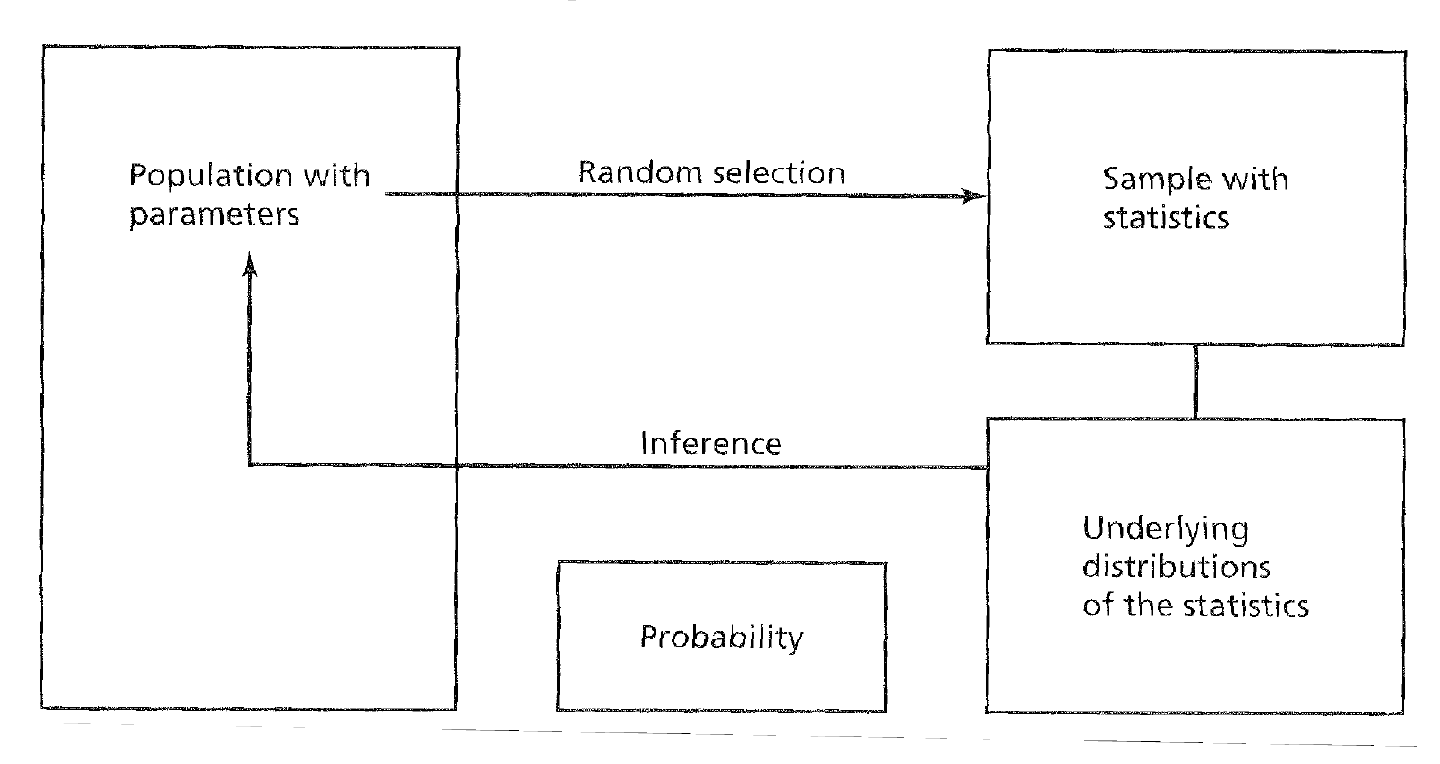
\includegraphics{img/hickssampling1.png}
\caption{Sampling}
\end{figure}

It's important to note that there are three different distributions that
we typically talk about. Two you should be familiar with -- the
populatation and the sample. The third is the \textbf{sampling
distribution} which is a \textbf{distribution of sample means}. The
sampling distribution of the mean is generated by considering all
possible sample means of a given sample size.

As is demonstratd from the image below, in A we can see there is some
sort of distribution, then with one sample (notice the \(\bar{X}\)), we
now have one wide sample. As we increase that to \(N = 16\), the
sampling distribution becomes more narrow. This narrowing is reflective
of the idea we are coming in on the true value of the population via our
random sampling. 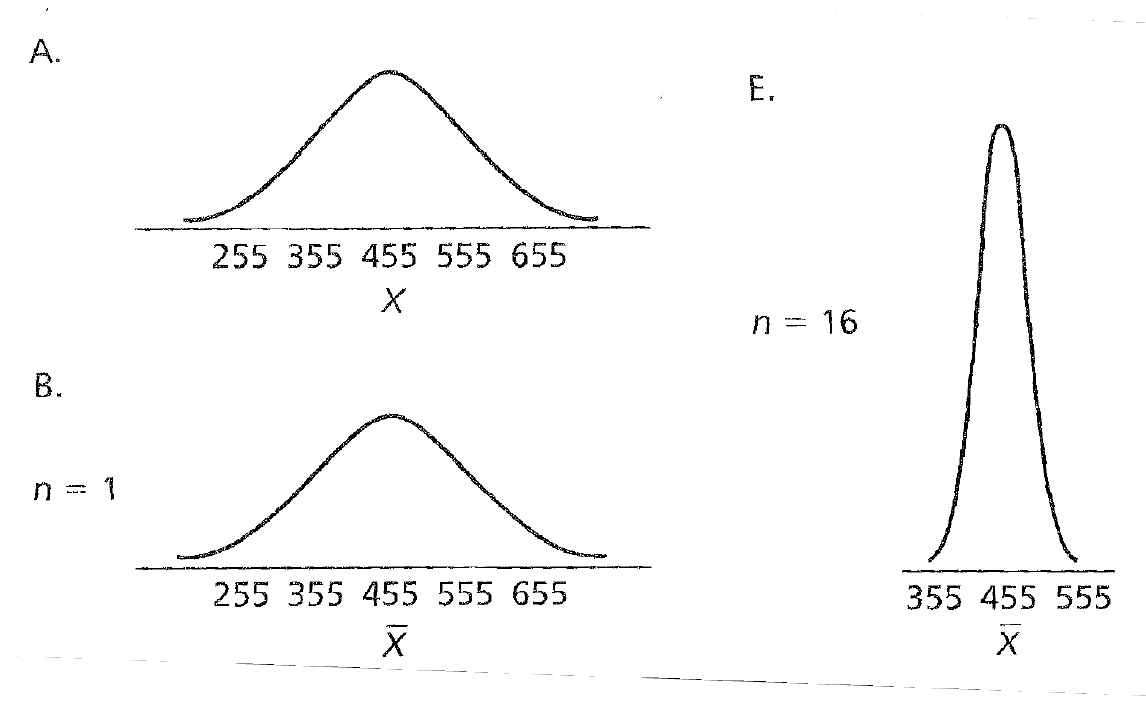
\includegraphics{img/hickssampling2.png}

The central limit theorem states that as the sample size \(n\)
increases, the sampling distribution of the mean for simple random
samples of \(n\) cases, taken from a population with a mean equal to
\(\mu\) and a finite variance equal to \(\sigma^2\), approximates a
normal distribution. From this, three points follow:

1.The shape of the sampling distribution is normal 2. The mean of the
sampling distribution is \(\mu\) 3. The standard deviation of the
sampling distribution, or standard error of the mean, is
\[\frac{\sigma}{\sqrt{n}}= \sigma_\bar{X}\]

Several important implications follow from an understanding of the
sampling distribution as a normal distribution and from the central
limit theorem.

Because we know the mean and standard error, we can calculate the
probability of selecting a random sample mean that is at or more extreme
than a particular value on the distribution.

\[z = \frac{\bar{X}-\mu}{\sigma_\bar{X}}\]

We can appeal to the table of z scores on the standard normal
distribution to find the probability.

For example, consider a sampling distribution of SAT scores with a mean
of 455 and a standard error of 8.33. This standard error was generated
with \(n\)= 144 and \(\sigma\)= 100.

So if you wanted to find the liklihood of finding as ample mean equal to
or more than extreme of 480, we would plug it into the follow equation.
\[z = \frac{480 - 455}{8.33} = 3.00\] And if we look that up a table of
z distributions, we got a probability of \(p=.0013\).

\begin{figure}
\centering
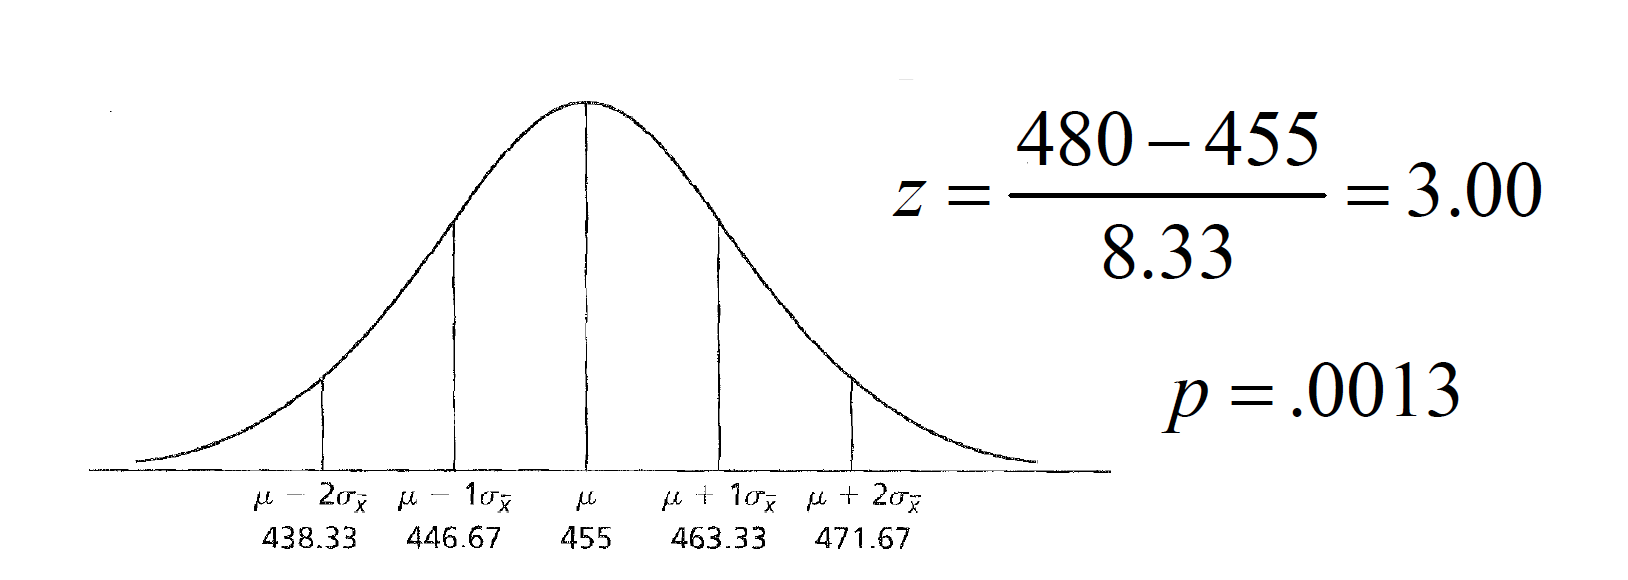
\includegraphics{img/hickssampling3.png}
\caption{Sampling}
\end{figure}

Because we know the mean and standard error, we can calculate the
probability of selecting a random sample mean that is at or more extreme
than a particular value on the distribution.

As sample size (\(n\)) increases, the variability of the sampling
distribution (\(\sigma_\bar{X}\)) decreases.

Even when the parent population is not normally distributed, the
sampling distribution becomes normal as sample size (n) increases.

You can see this demonstrated in THIS LINK.

\chapter{Hypothesis Testing}\label{hypothesis-testing}

The sampling distribution of the mean helps us to make hypotheses about
the likelihood that a given sample mean comes from a sampling
distribution with a given mean.

Stated differently, a hypothesis test helps us determine whether the
observed difference between a sample mean and a hypothetical population
mean is either negligible or meaningful.

The Null Hypothesis \(H_o : \mu = some value\) The alternative
Hypothesis \(H_o : != \mu = some value\)

The Alternative Hypothesis

A sample mean of a given sample size is produced and compared to the
hypothetical sampling distribution's mean to test the null hypothesis

Imagine we know the population (for some reason) and the True value is
455.

\begin{figure}
\centering
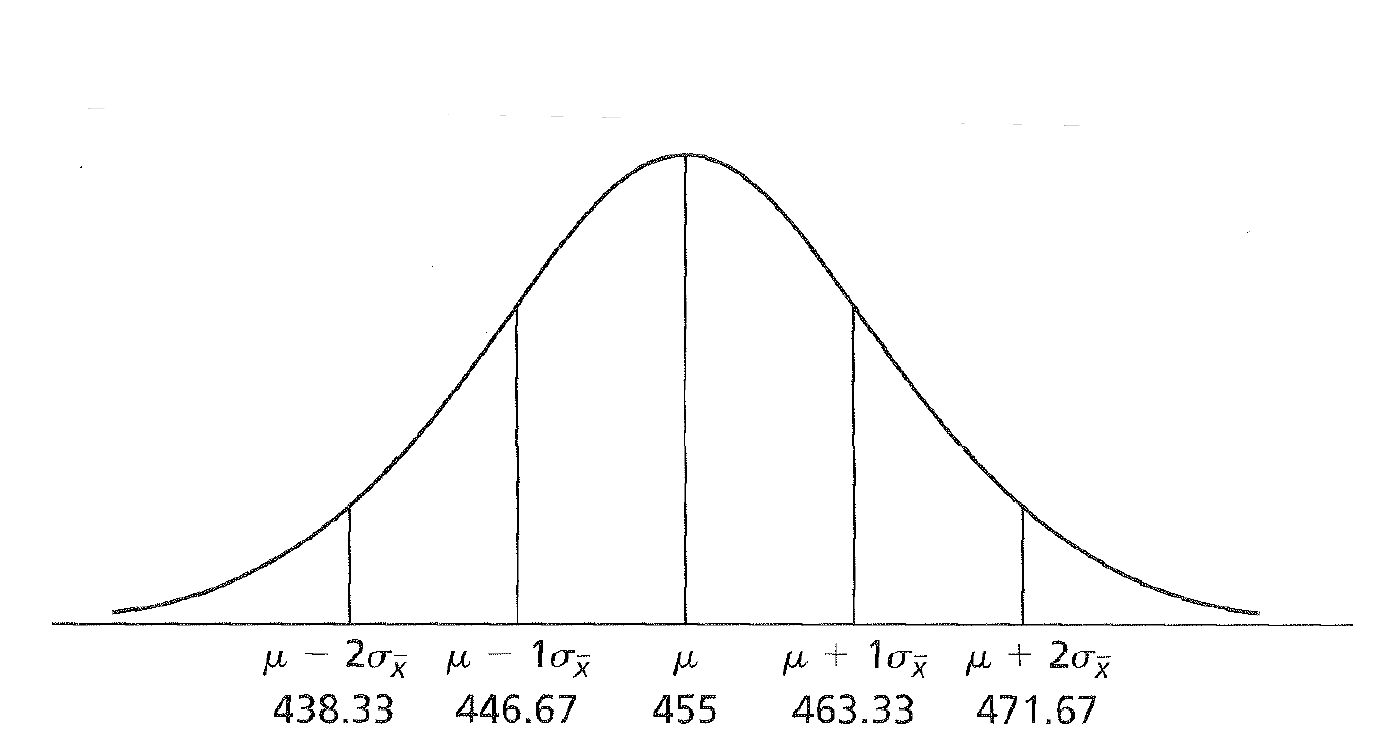
\includegraphics{img/hicksonesample1.png}
\caption{True Value is 455}
\end{figure}

\begin{figure}
\centering
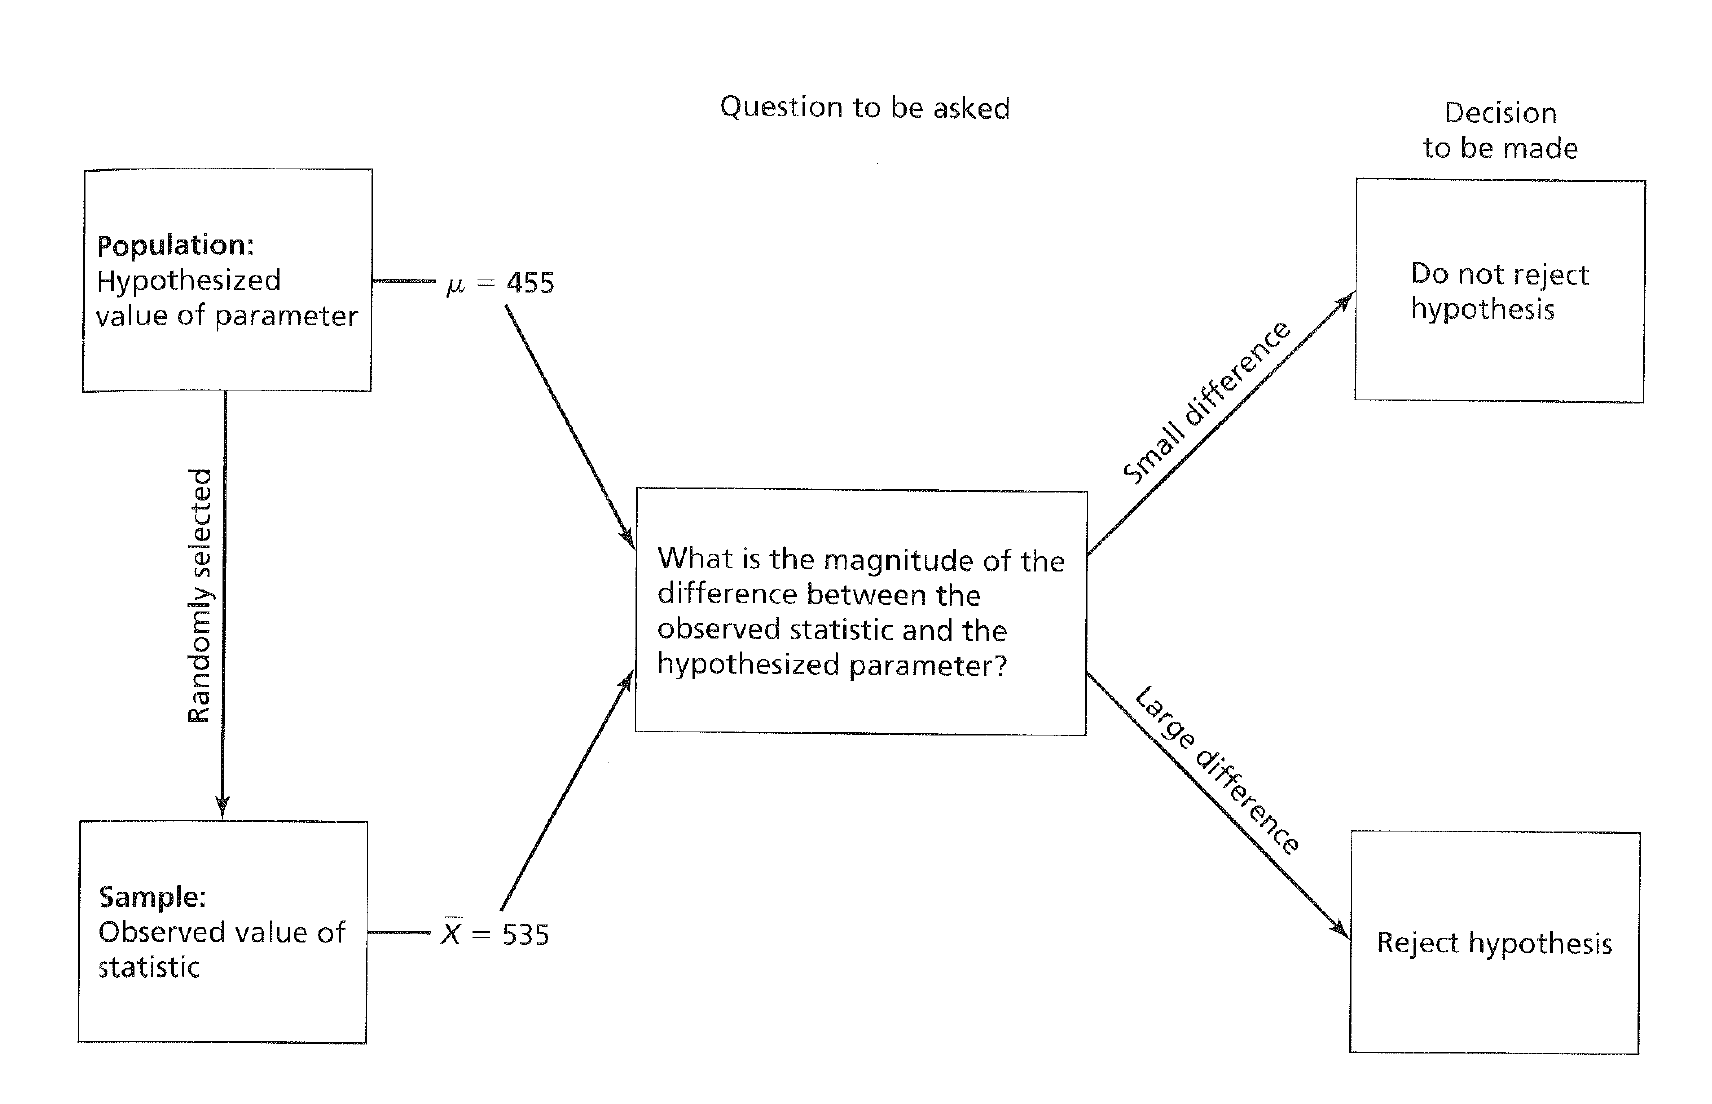
\includegraphics{img/hicksonesample2.png}
\caption{Descision Tree}
\end{figure}

The hypothesis test is based on inference (i.e., inductive reasoning),
and therefore there is a chance that mistaken inferences will be made.

The 2 ×2 matrix of decision outcomes given the state of nature and the
decision made

\begin{figure}
\centering
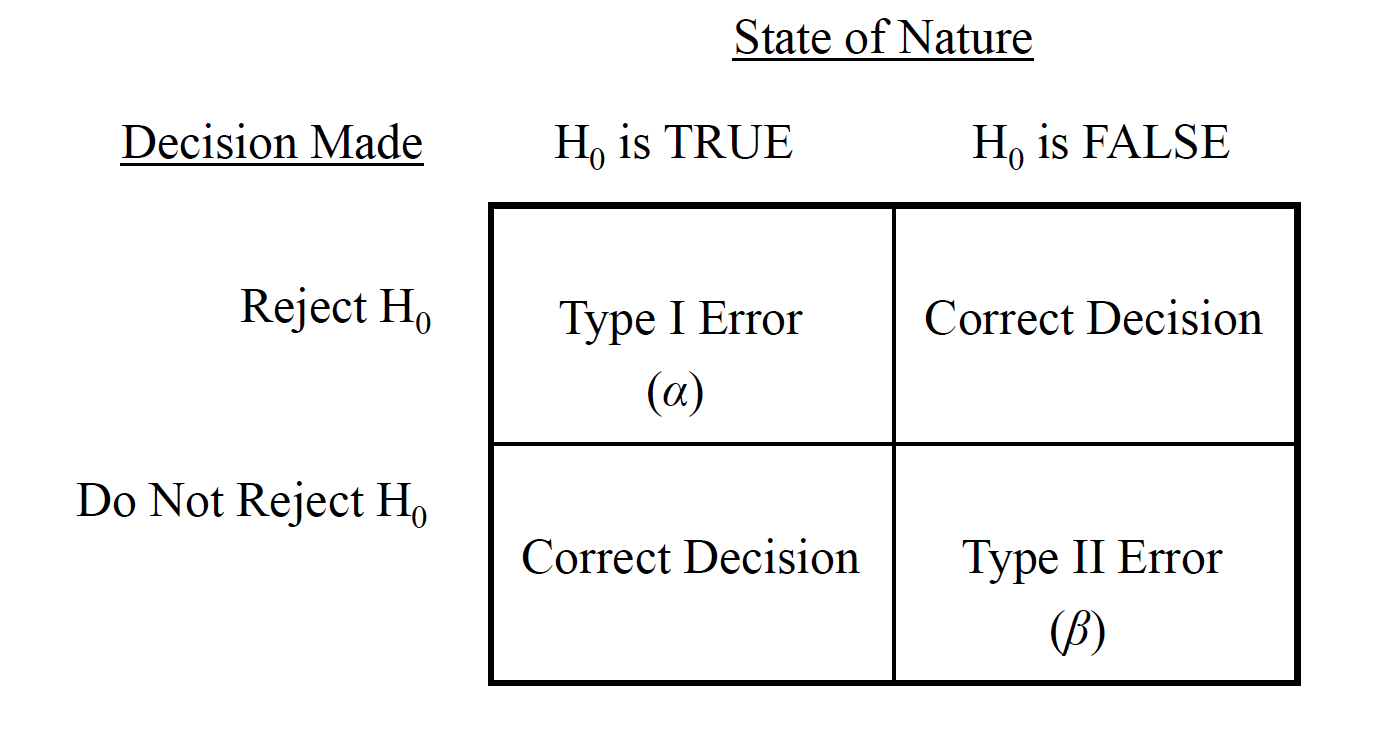
\includegraphics{img/hicksonesample3.png}
\caption{Matrix}
\end{figure}

A Type I erroris produced when we mistakenly reject the null. It is
associated with probability alpha (\(\alpha\)), or the level of
significance.

We conventionally set this level to be .05in psychology, but there are
considerations to be made for increasing or decreasing this value (e.g.,
.01 or .10).

A Type II erroris produced when we mistakenly fail to reject the null.
It is associated with probability beta (\(\beta\)), which is related to,
but not the same as, alpha.

The level of significance creates the bounds for the rejection
region---the extreme region(s) under the sampling distribution equal to
αif the null hypothesis is true.

\begin{figure}
\centering
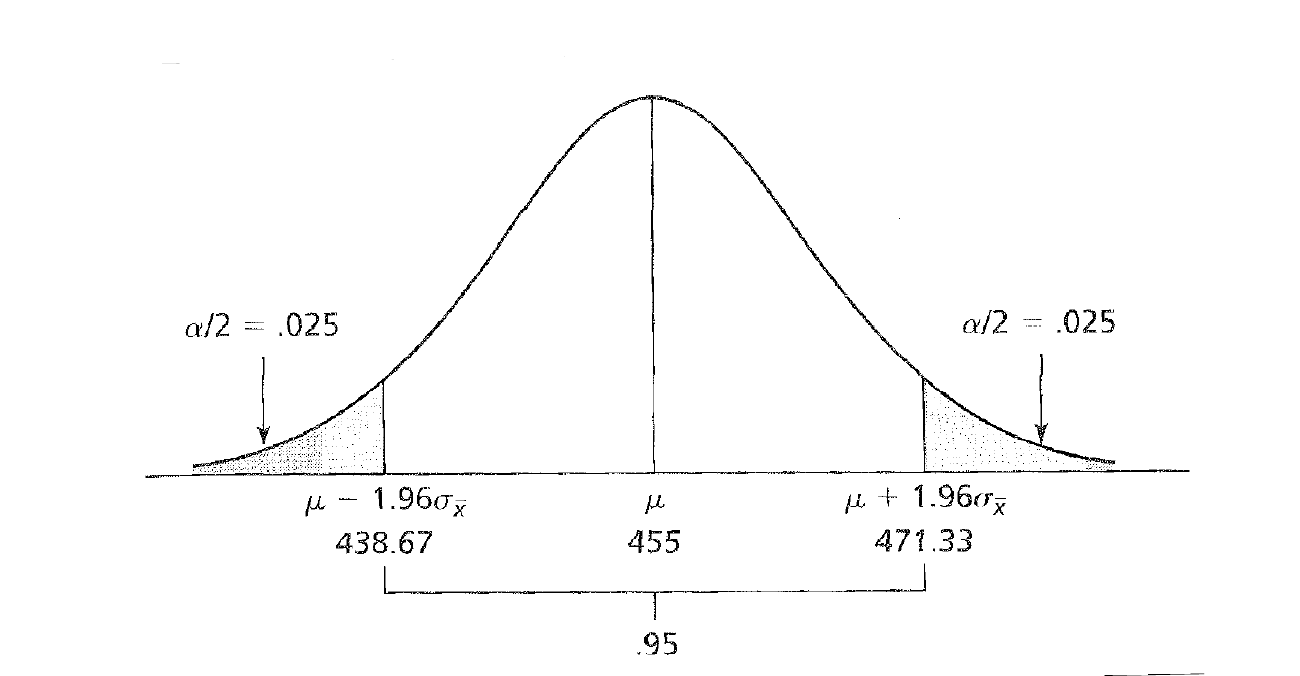
\includegraphics{img/hicksonesample4.png}
\caption{Matrix}
\end{figure}

The directionality of the test should also be considered.

\begin{figure}
\centering
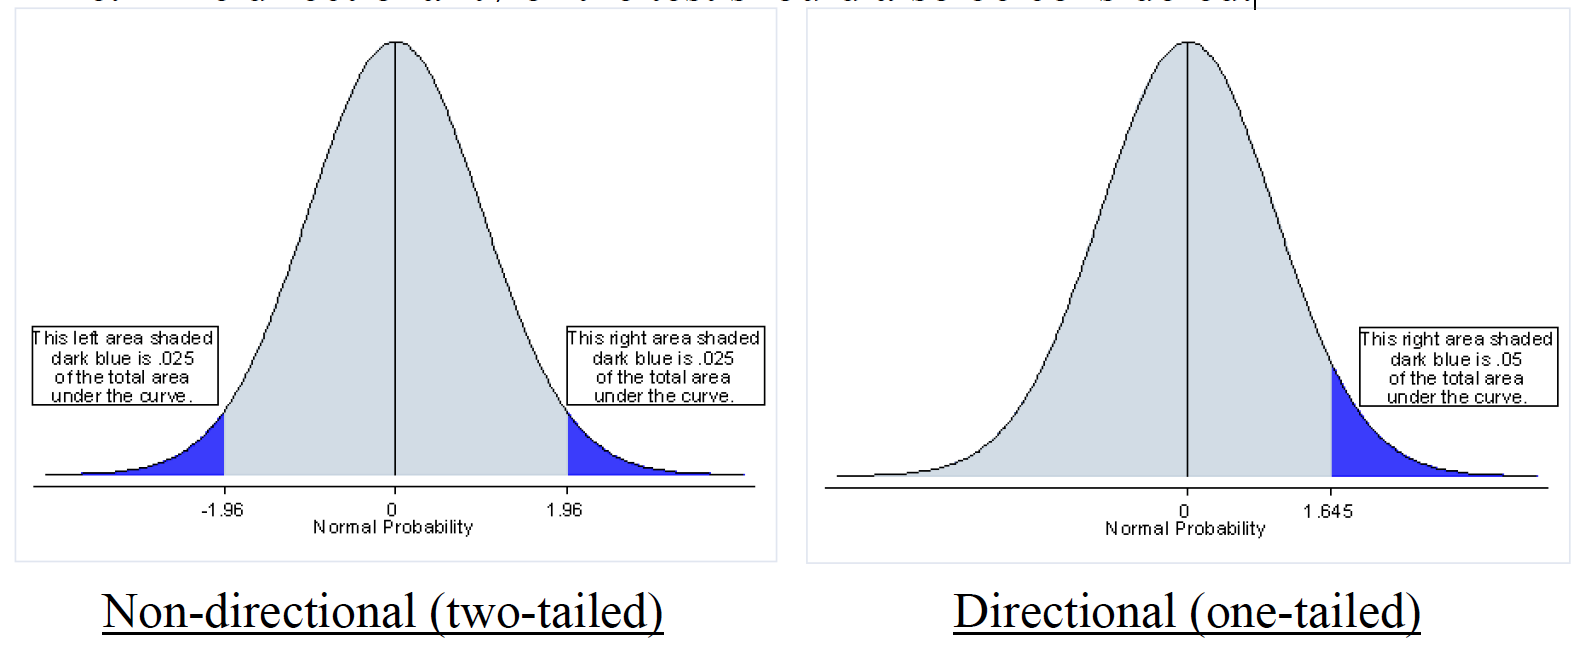
\includegraphics{img/hicksonesample5.png}
\caption{Matrix}
\end{figure}

Hypothesis tests differ slightly when population parameters, such as
\(\sigma^2\), are known versus unknown.

The general formula for a test statistic \(Statistic - parameter /SE\)

When \(\sigma^2\)is known, we use the standard error of the normal
distribution as the denominator. The result is the ztest.

Z TEST FORMULA

STANDARD ERROR HERE

When \(\sigma^2\) is unknown, we use the t distributionas our sampling
distribution, with a standard error that must be estimated from \(s^2\)
or \(s\). The result is the ttest.

T TEST AND STANDARD ERROR FORMULA HERE

Left off on Page 11 in onesampleNHST.png

The concept of degrees of freedom (df)must be considered for the ttest.
For each sample drawn, df= n--1.

VARIANCE FORMULSA

\begin{figure}
\centering
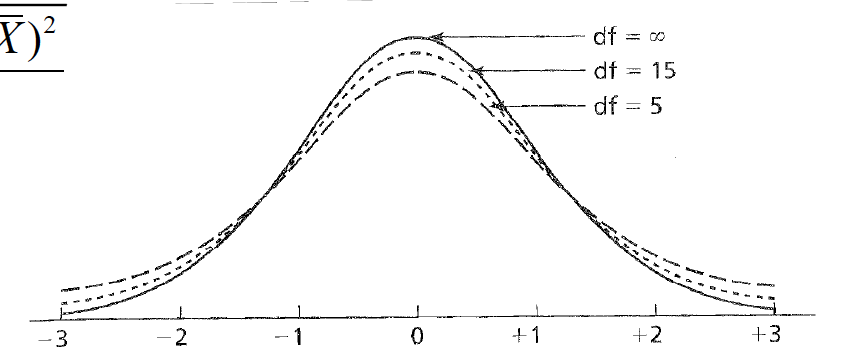
\includegraphics{img/hickssampling5.png}
\caption{DF on t statistic}
\end{figure}

\section{Steps of Hypothesis Testing}\label{steps-of-hypothesis-testing}

On a standardized anagram task, \(\mu\)= 26 anagrams solved with a
\(\simga\)= 4. A researcher tests whether the arousal from anxiety is
distracting and will decrease performance. A sample of \(n\)= 14 anxiety
patients is tested on the task. There average performance is 23.36
anagrams.

Step one: State the null and alternative hypotheses

\$H\_O = : \mu = 26 \$ \$H\_O = : \mu != 26 \$

Consider directionality.

Step two: Set the criterion for rejecting H0. Alpha is usually set to
.05, but could be other values depending on the research context. Again,
directionality is important to consider.

Step three: Select the sample and collect your data.

Step four: Locate the region of rejection and the critical value(s) of
your test statistic. Again, directionality is important to consider.

Step five: Compute the appropriate test statistic. σis known, so we use
the ztest.

\begin{figure}
\centering
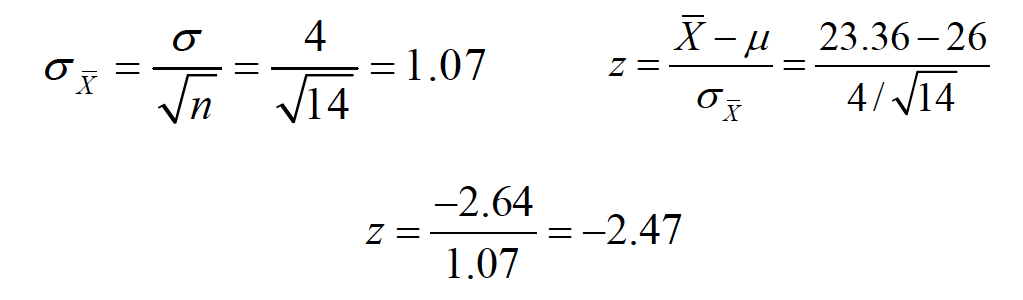
\includegraphics{img/hickssampling6.png}
\caption{Convert me}
\end{figure}

\begin{figure}
\centering
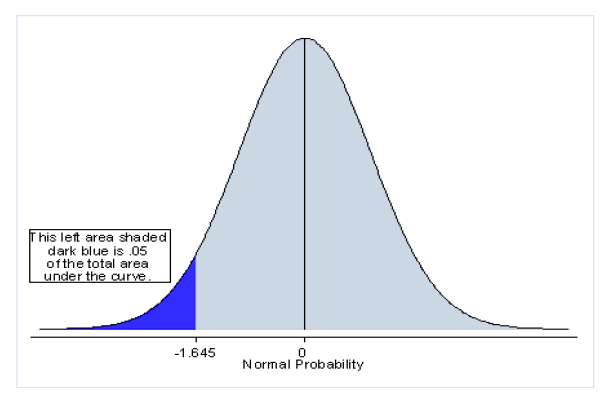
\includegraphics{img/hickssampling7.png}
\caption{Convert me}
\end{figure}

Step six: Decide whether to reject H0. Is -2.47 more extreme than the
critical value?

Step five: Compute the appropriate test statistic. \(\sigma\) is
unknown, so we use the ttest.

Step six: Decide whether to reject H0. Is -3.00 more extreme than the
critical value? df= 13, look up critical value in table C.3 and find
±1.77.

T distribution here

How do we report this result in a typical research article? ``The mean
number of anagrams solved by anxiety patients (M= 23.36) was
significantly lower than the mean established by test norms (M= 26),
t(13) = 3.00, p\textless{} .05.'' Sometimes you'll find people report
the pvalue lower than .01 if it passes this criterion as well. For
example, t(13) = 3.00, p\textless{} .01. Don't be confused by the
meaning of this, however.

\subsection{Other important
considerations.}\label{other-important-considerations.}

The hypothesis test is a test of the NULL hypothesis, assuming that the
null is true. Thus, the test gives you the probability of your sample
mean being that different (or more) from the population mean by chance
IFFthe null is true.

Statistical significance is not the same as practical significance.

Being able to report the result of a hypothesis test statistically
versus being able to describe the result to a lay person. Relate the
inference back to the original research question!

\section{Two Sample}\label{two-sample}

In cases where we wish to compare two sample means, the hypothesis
testing logic is essentially the same as with the one-sample tests, with
some slight differences in the null hypothesis, in the sampling
distribution, and in the computation. When different people (or animals)
contributed to the two samples, the comparison distribution that
represents the null hypothesis is a sampling distribution of differences
between means. The hypothesis test is therefore referred to as an
independent-samples test.

When both sample means were produced by the same participants, we
conduct what is known as a dependent-samples test. This is a test of the
average difference between the scores in one condition and the scores in
another condition---thus, the unit of measurement is a difference score.

Nondirectional Null Hypothesis \$H\_O : \mu\_1 - \mu\_2 = 0 \textbar{}
H\_O : \mu\_1 = \mu\_2 \$ Nondirectional Alternative Hypothesis \$H\_a :
\mu\_1 - \mu\_2 != 0 \textbar{} H\_a : \mu\_1 = \mu\_2 \$

Directional Null Hypothesis \$H\_O : \mu\_1 \textgreater{} \mu\_2
\textbar{} \mu\_1 \textless{} \mu\_2 \$ Directional Alternative
Hypothesis \$H\_a : \mu\_1 \textless{} \mu\_2 \textbar{} H\_a : \mu\_1
\textgreater{} \mu\_2 \$

\begin{figure}
\centering
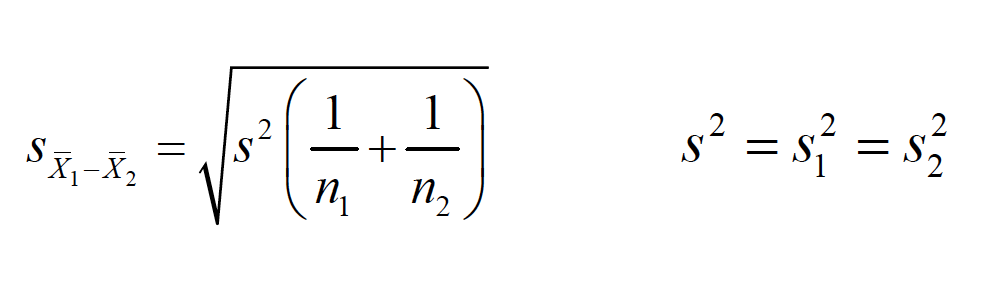
\includegraphics{img/hickssampling11.png}
\caption{Convert me}
\end{figure}

This is basically a subtraction of one sampling distribution from
another, to produce a distribution of possible differences between
sampling distributions. \$ \mu\_1 - \mu\_2\$ * The mean of this sampling
distribution is \$ \mu\_1 - \mu\_2\$ * The shape of this sampling
distribution is approximately normal. * When \sigma 2is known for each
distribution, the standard error of the difference between means is

s2is considered a pooled estimateof the population variance because the
individual estimates are literally summed together in the computation:

\(s^2 = \frac{SS_1 + SS_2}{n_1 + n_2 -2}\)

If you know the individual group variances or standard deviations, then

\(s^2 = \frac{(n_1 - 1)s_1^2 + (n_2 - 1)s_2^2}{n_1 + n_2 -2}\)

\begin{figure}
\centering
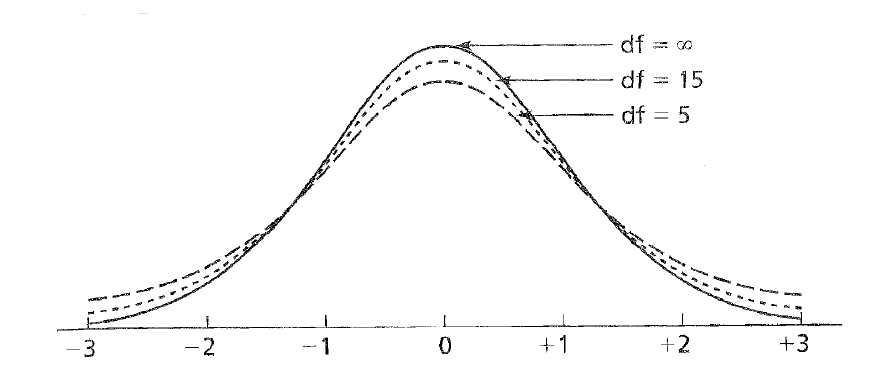
\includegraphics{img/hickssampling12.png}
\caption{Convert me}
\end{figure}

\(t = \frac{(\bar{X_1}-\bar{X_2})-(\bar{\mu_1}-\bar{\mu_2})}{s_{\bar{X_1}-\bar{X_2}}}\)

Example of the independent samples ttest

The instructor of an introductory psychology course is interested in
knowing if there is a difference in the mean grades on the final exam
between the fall and spring semester classes. Summary data for the two
samples is below:

\begin{figure}
\centering
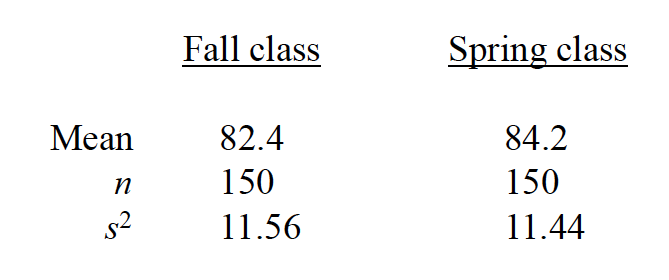
\includegraphics{img/hickssampling13.png}
\caption{Convert me}
\end{figure}

Are the final exam grades for the two classes equivalent?

Step one: State the null and alternative hypotheses
\(H_o:\mu_1 = \mu_2\) \(H_a:\mu_1 != \mu_2\)

b.Step two: Set the criterion for rejecting H0. Alpha is usually set to
.05, but could be other values depending on the research context. Make
sure you've considered directionality! c.Step three: Select the sample
and collect your data. d.Step four: Locate your region of rejection and
critical values.

Locate your region of rejection and critical values.

\(t_{cv,dv=298, \alpha=.05}= +/- 1.96\)

Step five: Compute the appropriate statistic. We were never given
\(\sigma\) or \(\sigma^2\), so we use the t test.

\begin{figure}
\centering
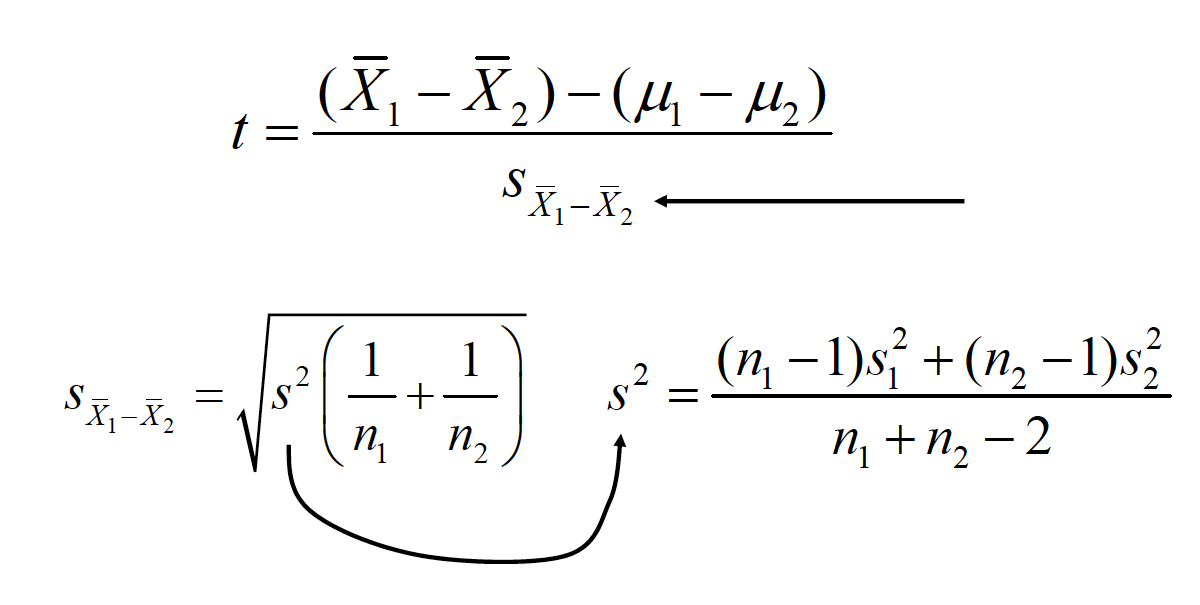
\includegraphics{img/hickssampling14.png}
\caption{Convert me}
\end{figure}

\begin{figure}
\centering
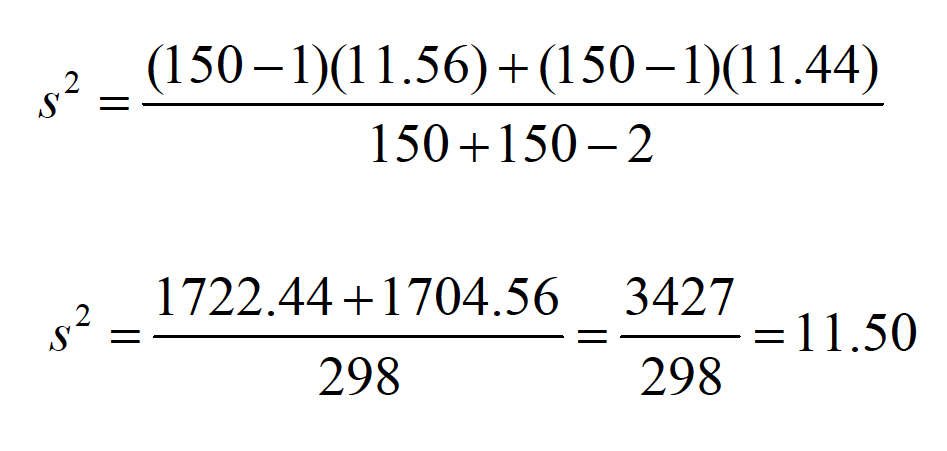
\includegraphics{img/hickssampling15.png}
\caption{Convert me}
\end{figure}

\begin{figure}
\centering
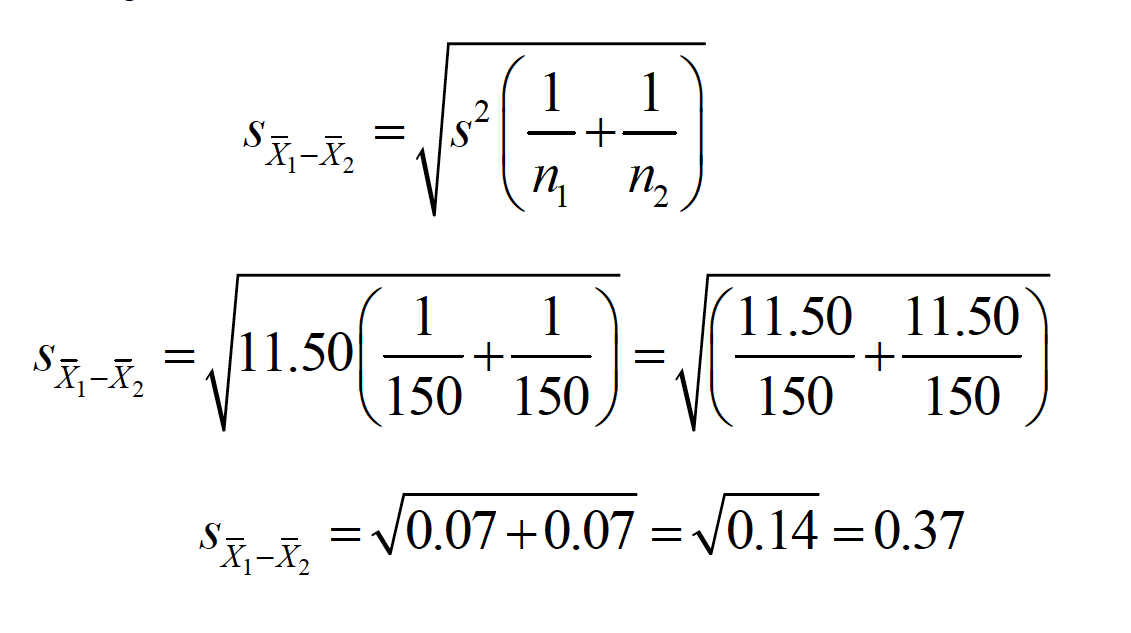
\includegraphics{img/hickssampling16.png}
\caption{Convert me}
\end{figure}

\begin{figure}
\centering
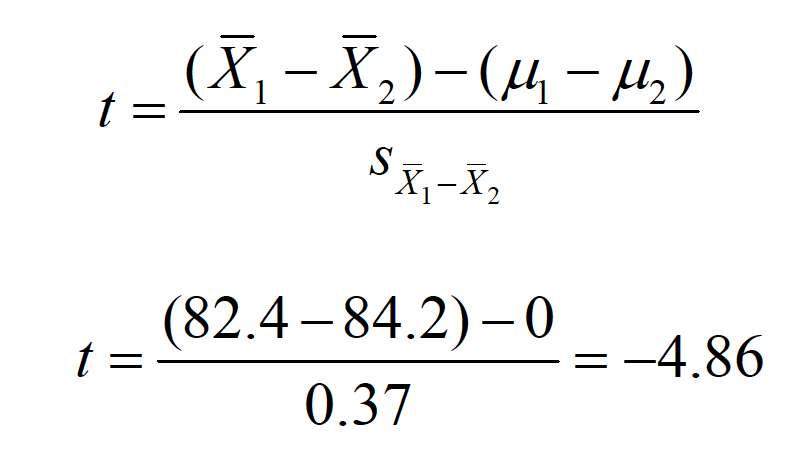
\includegraphics{img/hickssampling17.png}
\caption{Convert me}
\end{figure}

Step six: Decide whether to reject H0. Is -4.86 more extreme than the
critical value?

\(t_{cv,dv=298, \alpha=.05}= +/- 1.96\)

The effect sizerefers to the magnitude of the phenomenon being tested
and is calculated as

\begin{figure}
\centering
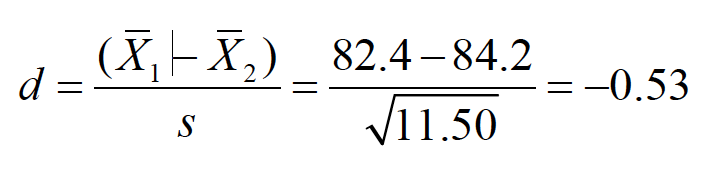
\includegraphics{img/hickssampling18.png}
\caption{Convert me}
\end{figure}

This statistic reflects the standardized distance between two
populationmeans. J. Cohen provides guidelines to interpret the value of
d:

``The average final exam score from the fall semester (M= 82.4) was
significantly lower than the average score from the spring semester (M=
84.2), t(298) = 4.86, p\textless{} .05.''

Small: = 0.25Medium: = 0.50Large: = 1.0

``The average final exam score from the fall semester (M= 82.4) was
significantly lower than the average score from the spring semester (M=
84.2), t(298) = 4.86, p\textless{} .05, Cohen's d= 0.53.''

\chapter{Power, Confidence Intervals, Effect Size
Measures}\label{power-confidence-intervals-effect-size-measures}

\section{Power}\label{power}

We have discussed the fact that the conclusions drawn from hypothesis
tests are essentially inferences about population parameters, based on
sample information. But we have thus far neglected a discussion of what
statistical factors should be considered in planning and assessing
research-based hypothesis tests.

By minimizing the probability of a Type II error (β), we are at the same
time increasing the amount of powerof our hypothesis test (1-β). Power
is defined as the probability of rejecting the null hypothesis when it
is false (i.e., should be rejected). Four important factors affect the
power of a statistical test.

Knowing any three of these factors mathematically fixes the fourth.
Thus, one can use these factors in determining the appropriate design
for a particular study. Sample size is most often the targeted factor in
formulating such a plan.

\begin{figure}
\centering
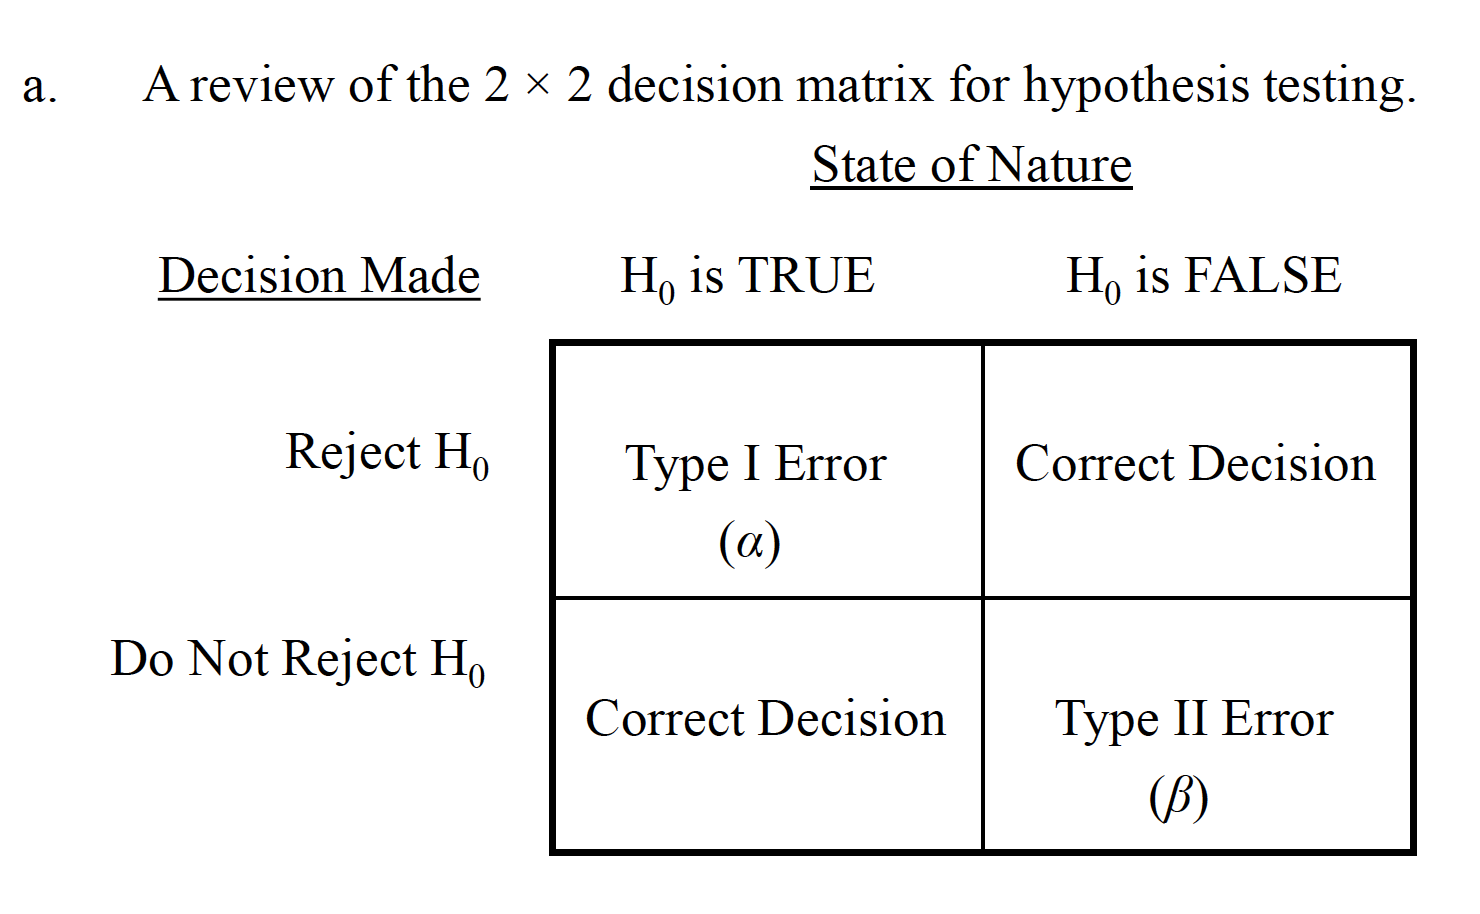
\includegraphics{img/hickspower1.png}
\caption{Table}
\end{figure}

Careful planning of research involves minimizing Type I andType II
errors. One rule of thumb is that \(\beta\) should be no more than .20
(e.g., if \(\alpha\) = .05, \(\beta\) = .20). c.For the t test, if the
null hypothesis distribution is centered on a t value of 0, then the
noncentralt distribution represents the alternative hypothesis
distribution, centered on \(\delta\). -This represents the average t
value one would expect for a given effect size and sample size

\begin{figure}
\centering
\includegraphics{img/hickspower2.png}
\caption{Noncentral T}
\end{figure}

\subsection{Test Equations}\label{test-equations}

One Sample tests

\$ \delta = d\sqrt{n}\$ \(d = \frac{\bar{X}-\mu}{\sigma}\)
\(g = \frac{\bar{X}-\mu}{s}\)

Two sample tests

\(\delta = d\sqrt{\frac{n}{2}}\) \(d = \frac{\mu_1-\mu_2}{\sigma}\)
\(g = \frac{\bar{X_1}=\bar{X_2}}{s_p}\)

For unequal n

\(n_n = \frac{2n_2n_2}{n_1 + n_2}\)
\(g = t\sqrt{\frac{n_1 + n_2}{n_1n_2}}\)

\begin{figure}
\centering
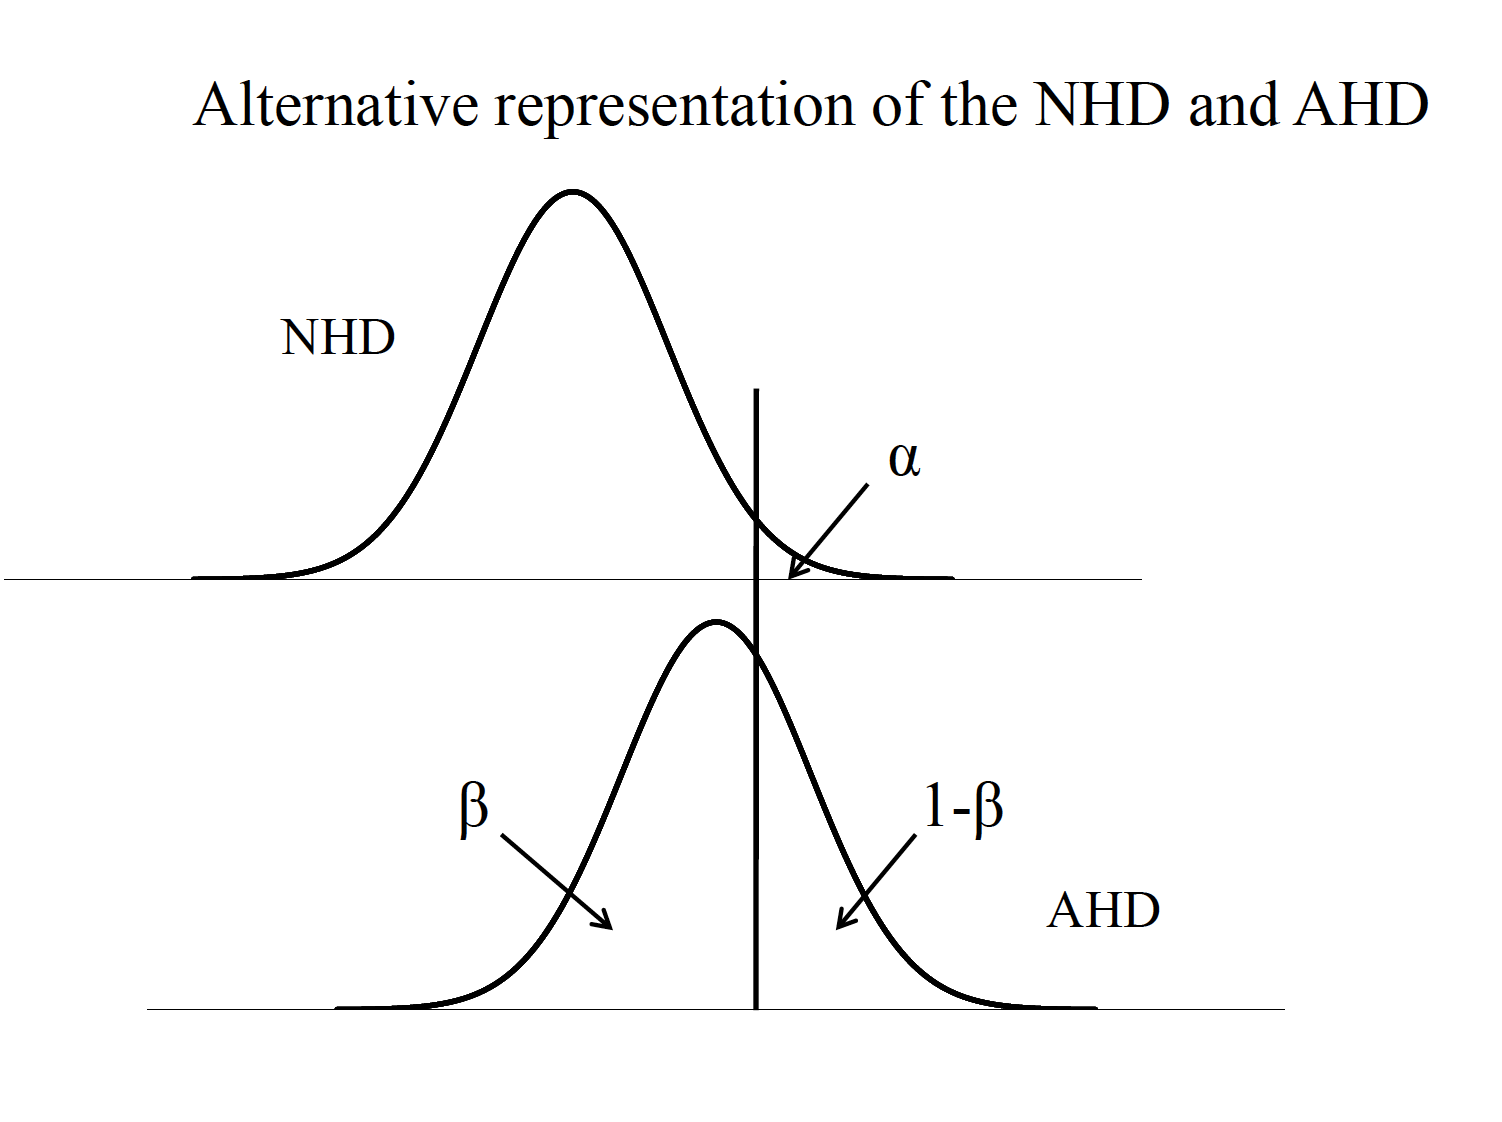
\includegraphics{img/hickspower3.png}
\caption{Noncentral T}
\end{figure}

Effect size (ES) or standardized effect size (e.g., d). i. The
difference between population means (e.g., \(\mu1-\mu2\)). ii. The
population standard deviation (\(\sigma\)).

\begin{figure}
\centering
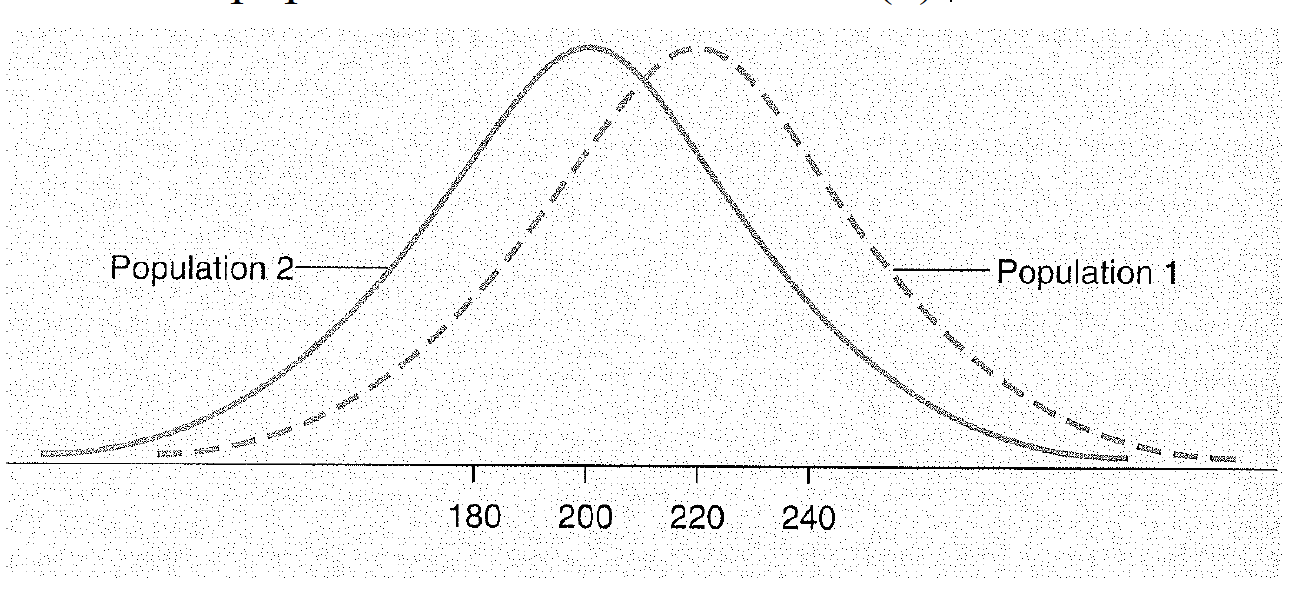
\includegraphics{img/hickspower4.png}
\caption{Noncentral T}
\end{figure}

\subsection{Factors of Power}\label{factors-of-power}

\begin{enumerate}
\def\labelenumi{\arabic{enumi}.}
\tightlist
\item
  Effect size (ES) or standardized effect size (e.g., d). \emph{The
  difference between population means (e.g., \(\mu_1-\mu_2\)). }The
  population standard deviation (\(\sigma\)).
\item
  Sample size (\(n\)).
\item
  Significance level (\(\alpha\)).
\item
  Directionality of the hypothesis test (one-tailed vs.~two-tailed).
\end{enumerate}

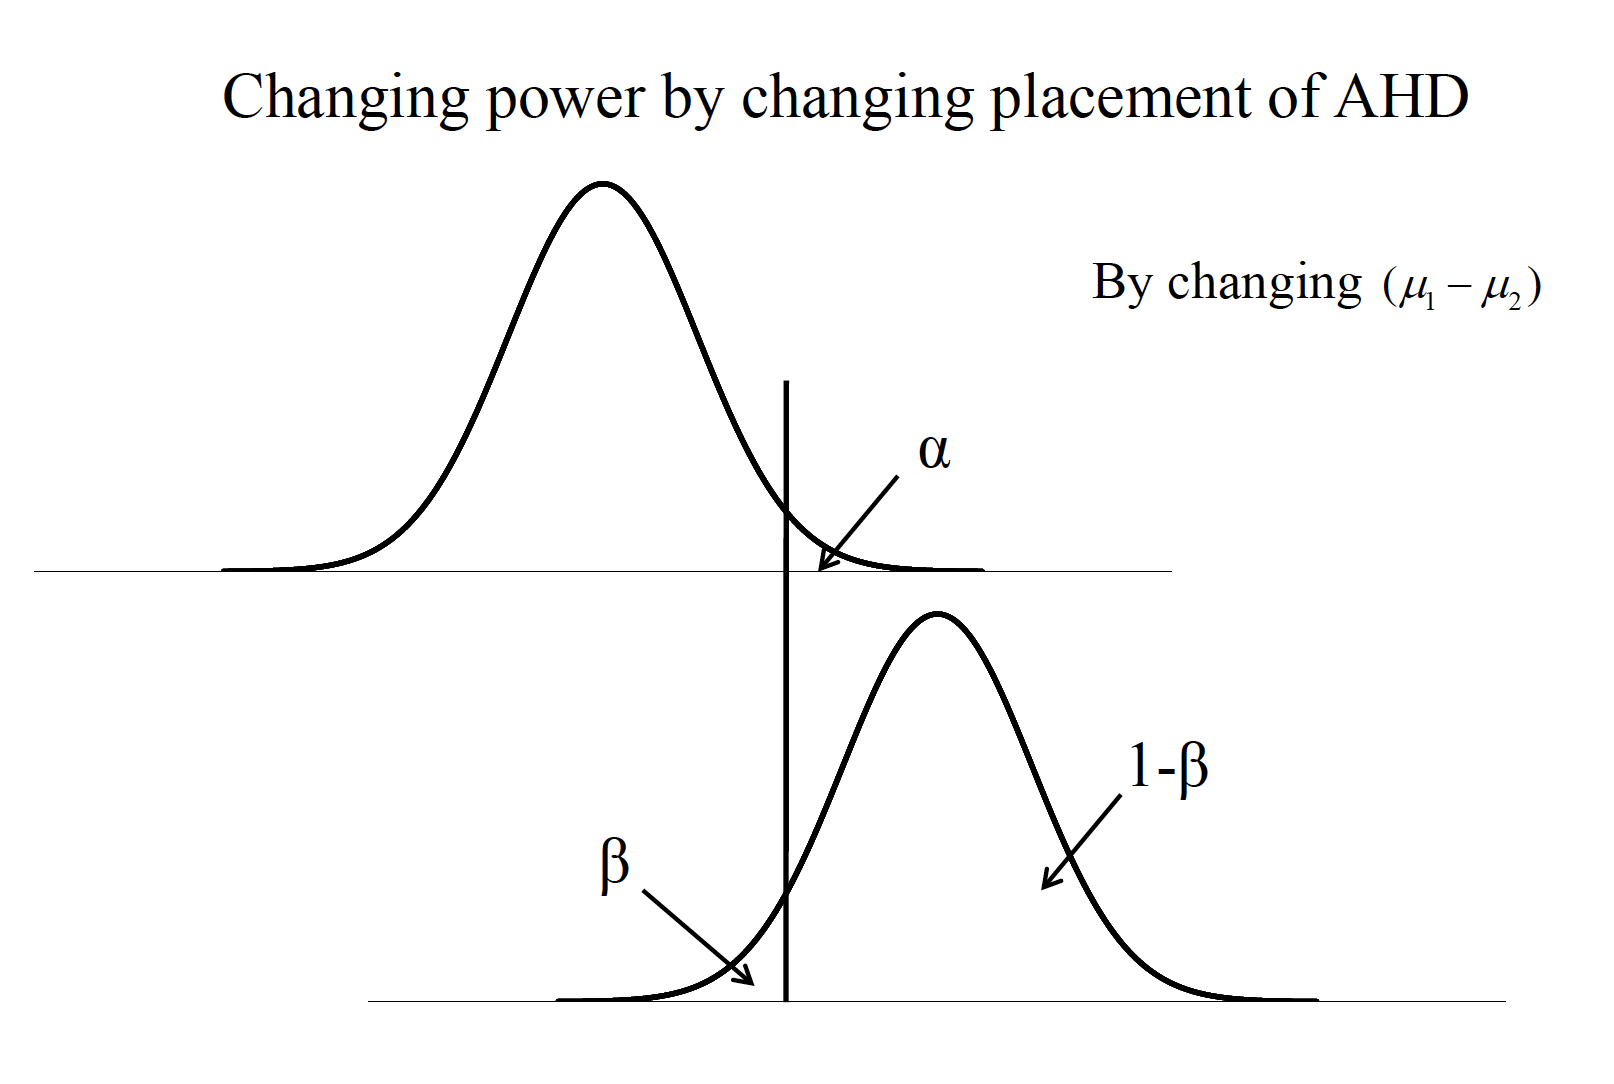
\includegraphics{img/hickspower5.png}
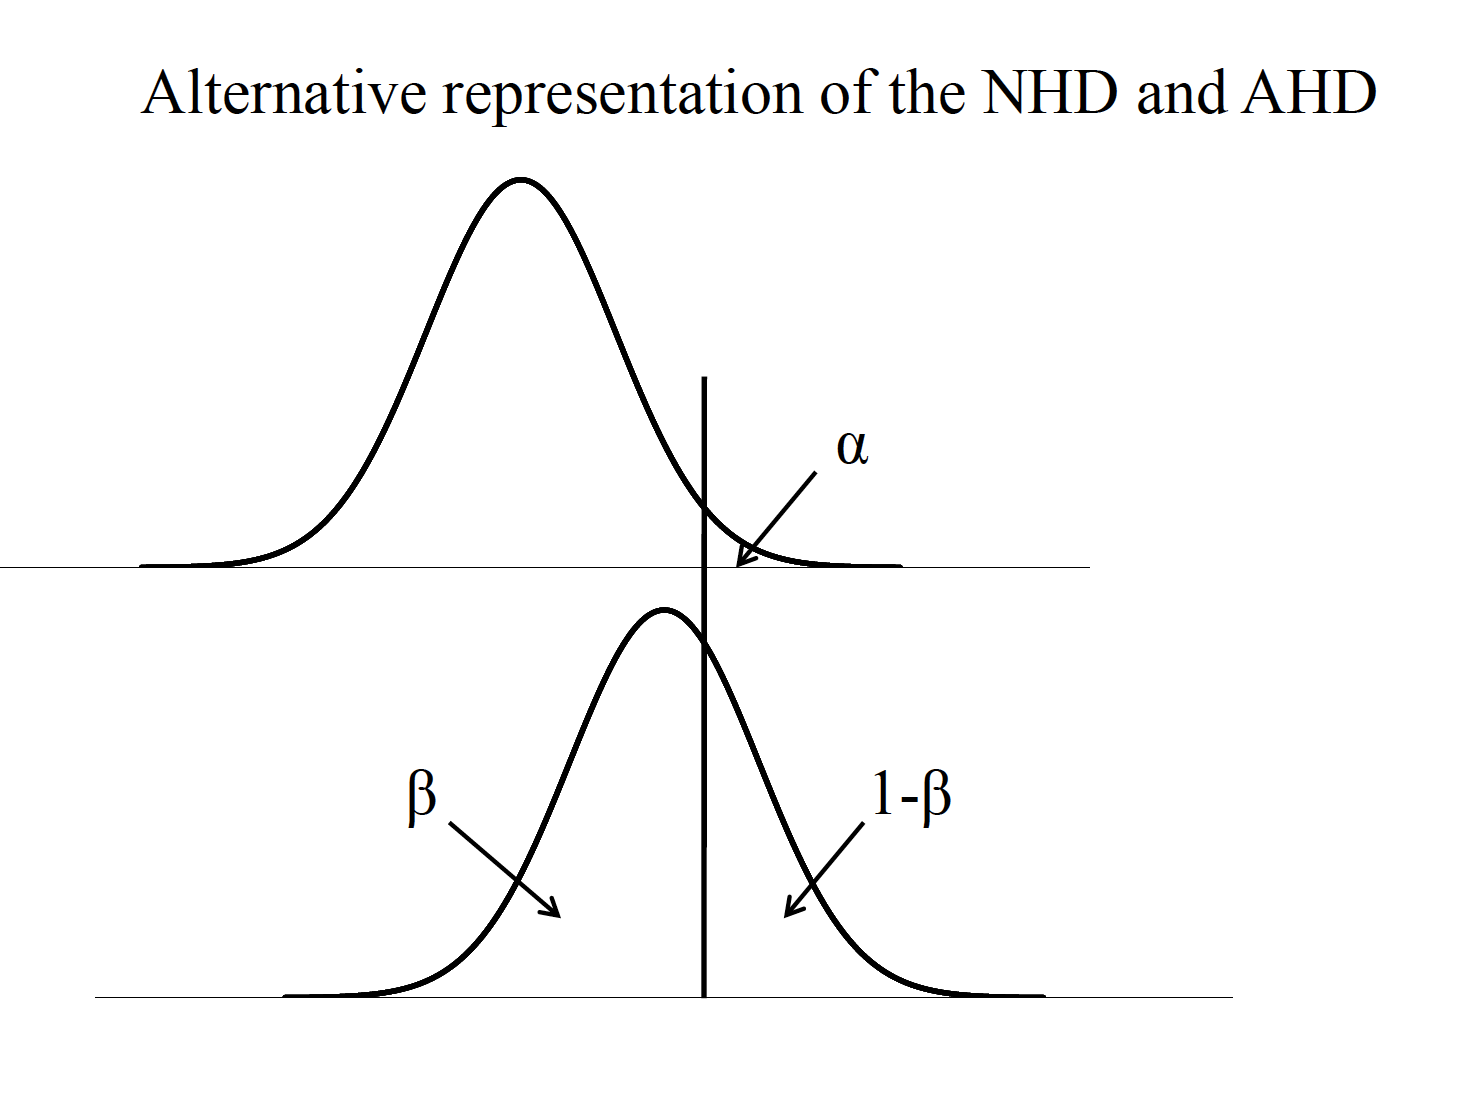
\includegraphics{img/hickspower6.png}
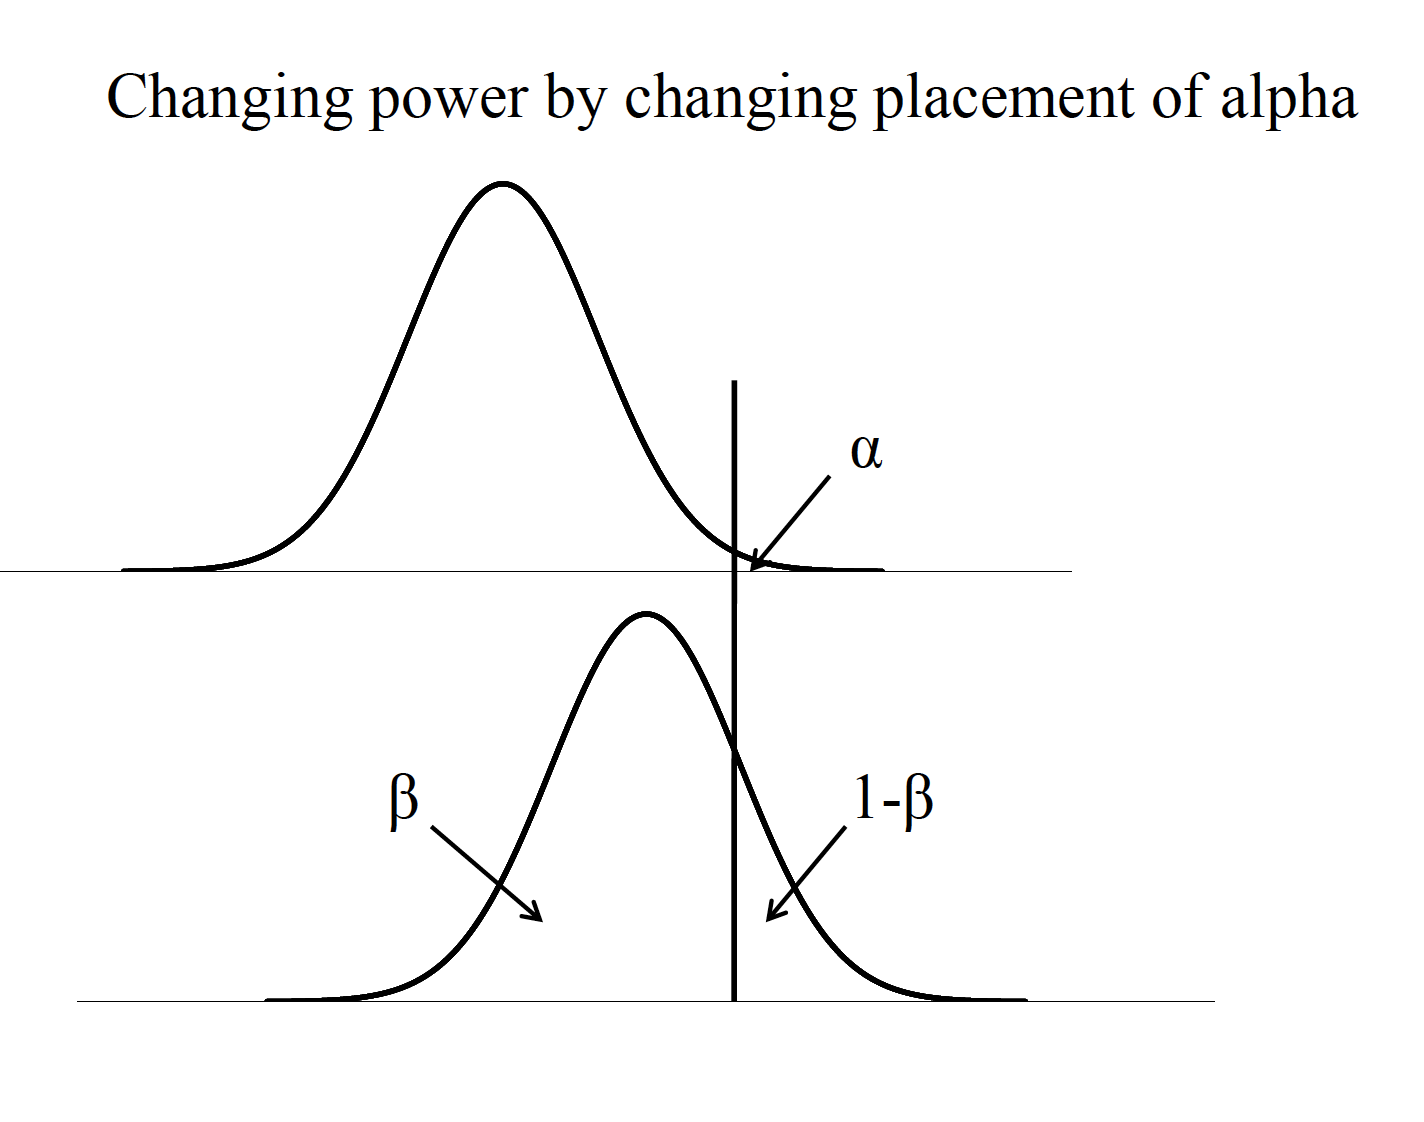
\includegraphics{img/hickspower7.png}
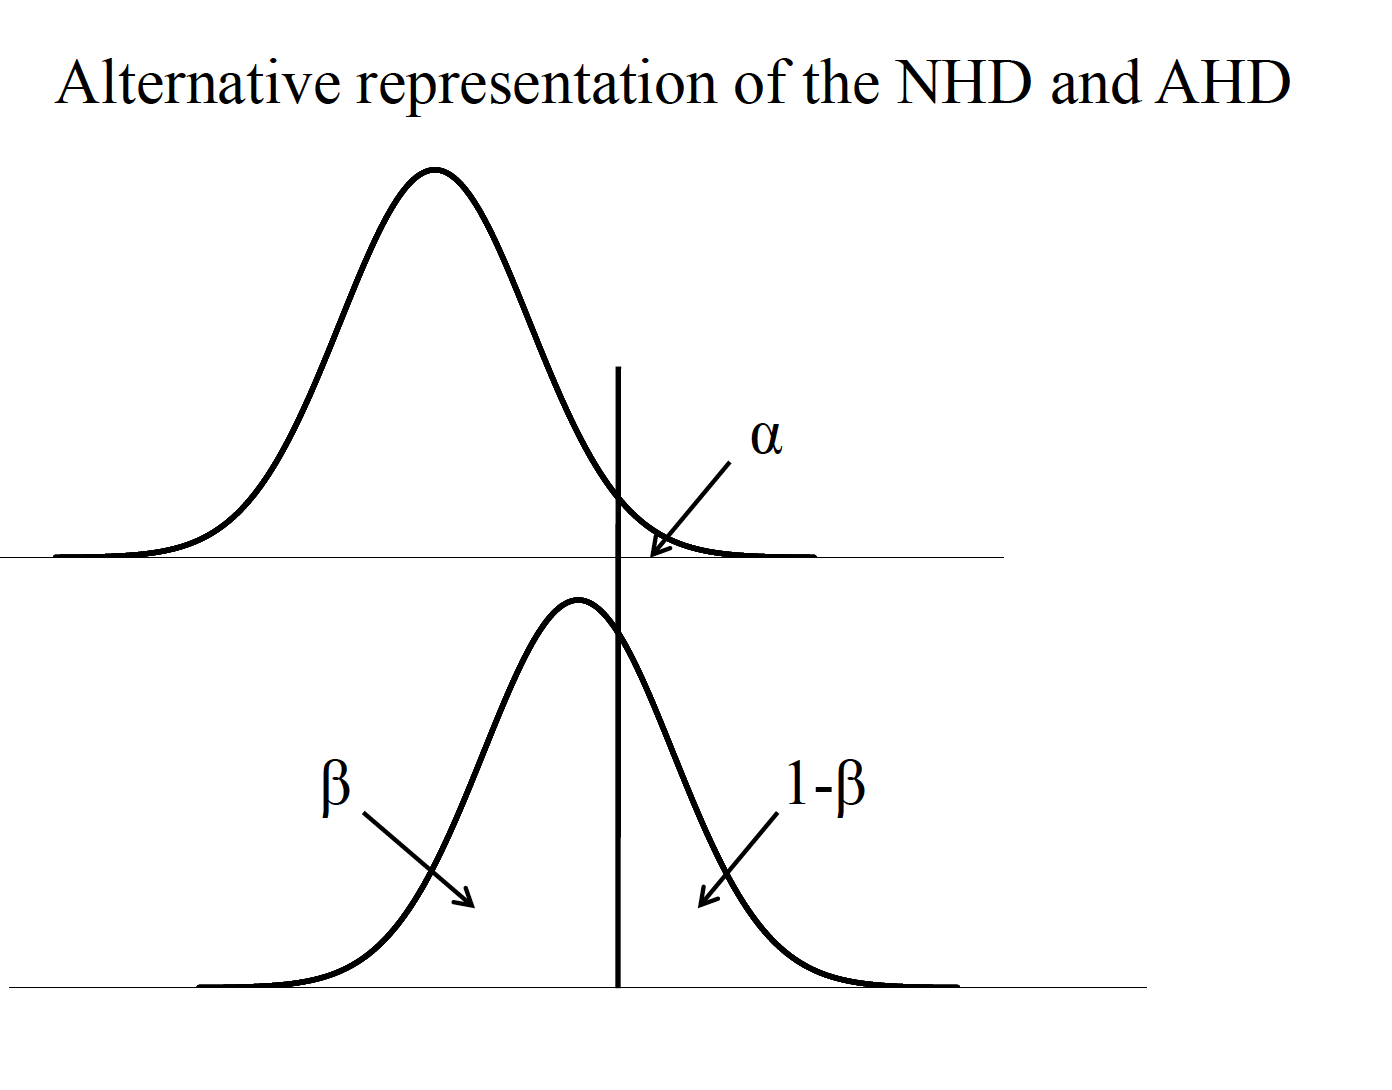
\includegraphics{img/hickspower8.png}
\includegraphics{img/hickspower9.png}

One sample case

\(\delta = d\sqrt{n}\) \(n = (\frac{\delta}{d})^2\)

two sample case

\(delta = d\sqrt{\frac{n}{2}}\) \(n = 2(\frac{\delta}{d})^2\)

A clinical psychologist wants to test the hypothesis that people who
seek treatment for psychological problems have higher IQs than the
general population. To test her hypothesis, she wants to use the IQ
values from 25 randomly selected clients and also to calculate the power
to find a 5-point difference in IQ. The mean of the population would be
100 and, therefore, the mean of her clients a 105. The population SD for
IQ is 15. (This scenario is from Howell's 2002 text ``Statistical
Methods for Psychology'')

Known: \(\mu_{client}=105\) \(\mu_{pop}\) \(\sigma_{pop} = 15\)

Calculate it with

\(d = \frac{105-100}{15} = 0.33\)

\(\delta = d\sqrt{n} = 0.33\sqrt{25}=1.65\)

Given this information and an expected alpha (two-tailed) of .05, we can
find in Table A.4 in the Cohen text that the power is between .25 and
.50, and more exactly about halfway in between (around .38). What does
this value of .38 mean?

If power should be at or above .80, what does the clinician do? Increase
alpha? Decrease the population SD? Increase the difference between
population means? Increase sample size? For a power level of .80, δneeds
to be 2.80, from Table A.4

\(n = (\frac{\delta}{d})^2=(\frac{2.80}{0.33}^2 = 8.48^2 = 71.91\)

\section{Confidence Ientervals}\label{confidence-ientervals}

\begin{enumerate}
\def\labelenumi{\arabic{enumi}.}
\item
  Sample measures of central tendency, such as the mean, are considered
  point estimates of population parameters. Confidence intervals are
  considered a type of interval estimation for population parameters.
\item
  Computation of confidence intervals.
\item
  Capture percentage, prediction, and replication
\end{enumerate}

Over repeated sampling from a known distribution, the confidence
interval represents the percentage of such intervals that contain the
population mean. Can be set at any percentage: 90\%, 95\%, 99\% Based on
characteristics of the sampling distribution (zor t) and therefore
highly related to the manner in which sampling distributions are used
for NHST  But CIs and pvalues from NHST are not the same thing!!!

\begin{figure}
\centering
\includegraphics{img/hicksci1.png}
\caption{Hicks CI 1}
\end{figure}

Confidence Interval for single sample mean

\(\bar{X} = +- (t_{cv})s_{\bar{X}}\)

Confidence interval for a mean difference scores (dependent samples)

\(\bar{D} +- (t_{cv})s_{\bar{D}\)

Confidence interval for a difference between sample means (independent
samples)

\((\bar{X_1}-\bar{X_2}) +- (t_{cv})(s_{\bar{X_1}-\bar{X_2}})\)

The instructor of an introductory psychology course is interested in
knowing if there is a difference in the mean grades on the final exam
between the fall and spring semester classes. Summary data for the two
samples is below:

What are the 95\% confidence intervals around each sample mean, and
around the difference between the sample means?

\begin{Shaded}
\begin{Highlighting}[]
\NormalTok{fall <-}\StringTok{ }\KeywordTok{c}\NormalTok{(}\FloatTok{82.4}\NormalTok{,}\DecValTok{150}\NormalTok{,}\FloatTok{11.56}\NormalTok{)}
\NormalTok{spring <-}\StringTok{ }\KeywordTok{c}\NormalTok{(}\FloatTok{84.2}\NormalTok{,}\DecValTok{150}\NormalTok{,}\FloatTok{11.44}\NormalTok{)}
\NormalTok{stat <-}\StringTok{ }\KeywordTok{c}\NormalTok{(}\StringTok{"Mean"}\NormalTok{,}\StringTok{"N"}\NormalTok{,}\StringTok{"s2"}\NormalTok{)}
\NormalTok{grades <-}\StringTok{ }\KeywordTok{data.frame}\NormalTok{(stat,fall, spring)}
\NormalTok{grades}
\end{Highlighting}
\end{Shaded}

\begin{verbatim}
##   stat   fall spring
## 1 Mean  82.40  84.20
## 2    N 150.00 150.00
## 3   s2  11.56  11.44
\end{verbatim}

What are the 95\% confidence intervals around each sample mean, and
around the difference between the sample means?

Confidence Interval for single sample mean

\(\bar{X} = +- (t_{cv})s_{\bar{X}}\)

This has critical value of 1.97 +-.

First need to find the standard error with each one.

\$s\_\bar\{X\} = \frac{s}{\sqrt{n}} = \frac{\sqrt{11.56}}{\sqrt{150}} =
\frac{3.4}{12.25}= 0.28 \$

\$s\_\bar\{X\} = \frac{s}{\sqrt{n}} = \frac{\sqrt{11.44}}{\sqrt{150}} =
\frac{3.4}{12.25}= 0.28 \$

Now do CI for both

\(\bar{X} = +- (t_{cv})s_{\bar{X}}\)

\(82.4 +- (1.97)(0.28)\) \(82.4 +- 0.55\) \((81.85, 82.95)\)

\(84.2 +- (1.97)(0.28)\) \(84.4 +- 0.55\) \((83.65, 84.75)\)

Calculate that now for differences

\((\bar{X_1}-\bar{X_2}) +- (t_{cv})(s_{\bar{X_1}-\bar{X_2}})\)

\(s_{\bar{X_1}-\bar{X_2}}= \sqrt{0.07 + 0.07} = \sqrt{0.14}=0.37\)

Alpha value associated with this is 1.96.

\(82.4 - 84.2) +- (1.96)(0.37)\) \(-1.8 +- 0.73 = (-2.53,-1.07)\)

Important points to keep in mind regarding confidence intervals:

\begin{enumerate}
\def\labelenumi{\arabic{enumi}.}
\tightlist
\item
  They are two-tailed by nature (i.e., on either side of a sample mean).
\item
  For a given sample size, increasing the level of confidence (e.g.,
  from 95\% to 99\%) increases the interval width.
\item
  The narrower the interval (at a given level of confidence!) reflects
  better statistical precision. Sample size directly affects the width
  of the interval by affecting the standard error estimate.
\end{enumerate}

\subsection{Capture Percentage}\label{capture-percentage}

Capture percentage, prediction, and replication What is the likelihood
that a subsequent experiment will replicate? Concept of capture
percentage: likelihood that a subsequent sample mean will fall into the
CI of the current sample.

\begin{figure}
\centering
\includegraphics{img/hicksci2.png}
\caption{Hicks CI 2}
\end{figure}

\chapter{Correlation and Regression}\label{correlation-and-regression}

\begin{enumerate}
\def\labelenumi{\arabic{enumi}.}
\tightlist
\item
  Statistical correlation simply refers to the notion that two variables
  are related to one another---when one varies, the other varies in a
  predictable manner. There are typically two ways to understand the
  nature of a correlation: visually and numerically.
\item
  There are multiple ways to understand and, therefore, calculate the
  Pearson correlation coefficient.
\item
  Relying on Pearson's rto describe a relationship assumes that certain
  conditions have been met.
\item
  Other factors may impact how one interprets the linear correlation.
\item
  Testing the ``significance'' of the correlation coefficient.
\item
  There is a correlation coefficient to deal with ordinal variables, or
  those measured by ranks.
\end{enumerate}

The variables are represented in the abstract as Xand Y.
b.Scatterplotsare figures that represent a pairof scores for each
individual, one score for each measured variable. The pattern of the
scatter indicates the nature of the relationship.

\begin{figure}
\centering
\includegraphics{img/hickscor1.png}
\caption{Hicks}
\end{figure}

\begin{figure}
\centering
\includegraphics{img/hickscor2.png}
\caption{Hicks}
\end{figure}

\begin{figure}
\centering
\includegraphics{img/hickscor3.png}
\caption{Hicks}
\end{figure}

The statistical representation of the correlation was developed by Karl
Pearson and is called the Pearson product-moment correlation
coefficient, or r.

\begin{enumerate}
\def\labelenumi{\roman{enumi}.}
\tightlist
\item
  r varies from -1 to 1.
\item
  The strength, or magnitude, of the relationship increases as distance
  from 0 increases. iii.The sign of the correlation represents the
  direction, or slopeof the relationship.
\end{enumerate}

\begin{figure}
\centering
\includegraphics{img/hickscor3.png}
\caption{Hicks}
\end{figure}

A graduate student samples 50 college professors in social sciences at
the same university who have been there for at least 10 years. She
measures them on a number of characteristics: average quality of their
instruction, average quality of their courses, number of publications,
and number of citations by other authors. Is there a relationship
between the number of publications and number of citations?

\begin{figure}
\centering
\includegraphics{img/hickscor4.png}
\caption{Hicks}
\end{figure}

\begin{figure}
\centering
\includegraphics{img/hickscor5.png}
\caption{Hicks}
\end{figure}

\section{Calculating Person C}\label{calculating-person-c}

One method is to examine the cross-products, which represent the
multiplication of Xand Y, usually on a standard scores. The result is
the standard score formula:

\begin{figure}
\centering
\includegraphics{img/hickscor6.png}
\caption{Hicks}
\end{figure}

Note these formulas (e.g., z-score) use population characteristics This
approach is very tedious, and does not make sense unless you already
have the z-scores calculated for some reason.

\begin{figure}
\centering
\includegraphics{img/hickscor7.png}
\caption{Hicks}
\end{figure}

The deviation score formulais a computational formula that relies on
using deviations from respective means:

\begin{figure}
\centering
\includegraphics{img/hickscor8.png}
\caption{Hicks}
\end{figure}

There is a raw score, computational formula that bypasses the need to
calculate deviations from each mean:

\begin{figure}
\centering
\includegraphics{img/hickscor9.png}
\caption{Hicks}
\end{figure}

Finally, we can use the covarianceto compute the correlation.

Covariance is the average sum of the cross-products of deviations:

\begin{figure}
\centering
\includegraphics{img/hickscor9a.png}
\caption{Hicks}
\end{figure}

Dividing this number by the cross-product of the unbiased sample
standard deviations produces:

\begin{figure}
\centering
\includegraphics{img/hickscor10.png}
\caption{Hicks}
\end{figure}

\subsection{Assumptions}\label{assumptions}

\begin{enumerate}
\def\labelenumi{\alph{enumi}.}
\tightlist
\item
  The scores are pairs---the same set of individuals needs to contribute
  both scores. b.Because the mean and variance are used to compute r,
  the variables need to be measured on an interval or ratio scale.
  c.Xand Yare normally distributed. d.The observations were randomly
  sampled. e.The relationship between the variables is linear, rather
  than curvilinear. Values of rare uninterpretable (and are
  underestimates) for curvilinear relationships.
\end{enumerate}

If the rangeon one or both variables is restricted(i.e., the group is
very homogeneous on Xand/or Y), then the value of rtends to become
smaller. Theoretically, the correlation can get bigger with range
restriction, although this is VERY rare with moderate-to-large sample
sizes.

\begin{figure}
\centering
\includegraphics{img/hickscor11.png}
\caption{Hicks}
\end{figure}

The sample size will not affect the value of r(except when N= 2), but
will affect its accuracyin terms of statistical significance. -when N=
2, rALWAYS equals ±1.0 c.The coefficient of determinationrepresents the
amount of variance in Ythat can be associated with the variance in X.

\begin{figure}
\centering
\includegraphics{img/hickscor12.png}
\caption{Hicks}
\end{figure}

Conceptual

\begin{figure}
\centering
\includegraphics{img/hickscor13.png}
\caption{Hicks}
\end{figure}

Finally, a measured correlation says nothing about whether Xand Yare
causally linked, only that there is an association. There are three
generic possible reasons for the association.

\begin{figure}
\centering
\includegraphics{img/hickscor14.png}
\caption{Hicks}
\end{figure}

Testing the ``significance'' of the correlation coefficient. a.Is the
correlation different from 0?

\begin{figure}
\centering
\includegraphics{img/hickscor15.png}
\caption{Hicks}
\end{figure}

Or look up critical values in A5 and compare with r 48df .05 alpha of
.273

\begin{figure}
\centering
\includegraphics{img/hickscor16.png}
\caption{Hicks}
\end{figure}

\begin{figure}
\centering
\includegraphics{img/hickscor17.png}
\caption{Hicks}
\end{figure}

There is a correlation coefficient to deal with ordinal variables, or
those measured by ranks, called Spearman rho.

\begin{figure}
\centering
\includegraphics{img/hickscor18.png}
\caption{Hicks}
\end{figure}

d= the difference between paired ranks, rather than paired scores.

\begin{figure}
\centering
\includegraphics{img/hickscor19.png}
\caption{Hicks}
\end{figure}

\chapter{Regression}\label{regression}

\begin{enumerate}
\def\labelenumi{\arabic{enumi}.}
\tightlist
\item
  Regression essentially involves creating a mathematical function that
  best describes the functional relationship between variables Xand Y.
  It is used in a two-step process: estimating the function for a full
  data set, and then applying it to a partial data set in which X, but
  not Y, is known (i.e., prediction).
\item
  There are different ways to compute the components of the regression
  line.
\item
  We can also identify aspects of the regression line that give us an
  idea about the accuracy of prediction.
\item
  We can test the significance of the regression coefficient (the slope)
  under the null hypothesis that the slope = 0. This is analogous to the
  null hypothesis test that the correlation = 0.
\end{enumerate}

Xis referred to as the predictorvariable and Yis referred to as the
criterionvariable.

The slope-intercept form of the line is (SLOPE OF LINE see slides) i.The
predictedscore on Yis ii.bis the slopeof the line iii.ais the
Y-interceptof the line; that is, where the line intercepts the Yaxis
when X= 0 ˆYbXa

We fit the ``best'' line to the data set by using the least
squaresprinciple---minimizing the summed, squared distance from each
data point to the line. i. Error (e) is represented by the distance from
each Y-point to the line.

\begin{figure}
\centering
\includegraphics{img/hicksreg1.png}
\caption{Hicks}
\end{figure}

When we have found the lowest possible total squared error, we have
identified the best-fitting line.

\begin{figure}
\centering
\includegraphics{img/hicksreg2.png}
\caption{Hicks}
\end{figure}

\begin{figure}
\centering
\includegraphics{img/hicksreg3.png}
\caption{Hicks}
\end{figure}

\begin{figure}
\centering
\includegraphics{img/hicksreg4.png}
\caption{Hicks}
\end{figure}

\begin{figure}
\centering
\includegraphics{img/hicksreg5.png}
\caption{Hicks}
\end{figure}

To find a predicted score for a data point, we simply substitute the
Xvalue into the prediction equation.

\begin{figure}
\centering
\includegraphics{img/hicksreg6.png}
\caption{Hicks}
\end{figure}

\begin{figure}
\centering
\includegraphics{img/hicksreg7.png}
\caption{Hicks}
\end{figure}

\begin{figure}
\centering
\includegraphics{img/hicksreg8.png}
\caption{Hicks}
\end{figure}

We can also identify aspects of the regression line that give us an idea
about the accuracy of prediction. a. The error in prediction (e) is
associated with its own distribution. The varianceof this distribution
(i.e., the `variance of the estimate') is

\begin{figure}
\centering
\includegraphics{img/hicksreg9.png}
\caption{Hicks}
\end{figure}

The standard deviation of this distribution is also called the standard
error of the estimate

\begin{figure}
\centering
\includegraphics{img/hicksreg10.png}
\caption{Hicks}
\end{figure}

\begin{figure}
\centering
\includegraphics{img/hicksreg11.png}
\caption{Hicks}
\end{figure}

We can also identify aspects of the regression line that give us an idea
about the accuracy of prediction

We can understand the standard error of the estimate in terms of the
conditional distributionof Yfor each value of X. Each conditional
distribution is assumed to have the same
variance---homoscedasticity---and to have a normaldistribution.

\begin{figure}
\centering
\includegraphics{img/hicksreg12.png}
\caption{Hicks}
\end{figure}

Because of these assumptions, we can make statements about the
probability of predicted scores defined by the regression line

What's the probability of Y around Yhat at anyscore of X?

\begin{figure}
\centering
\includegraphics{img/hicksreg13.png}
\caption{Hicks}
\end{figure}

\begin{figure}
\centering
\includegraphics{img/hicksreg14.png}
\caption{Hicks}
\end{figure}

\begin{figure}
\centering
\includegraphics{img/hicksreg15.png}
\caption{Hicks}
\end{figure}

\begin{figure}
\centering
\includegraphics{img/hicksreg16.png}
\caption{Hicks}
\end{figure}

Because of these assumptions, we can make statements about intervals
around true values of Yestimated by the regression line (prediction
intervals)

\begin{figure}
\centering
\includegraphics{img/hicksreg17.png}
\caption{note y hat}
\end{figure}

\begin{figure}
\centering
\includegraphics{img/hicksreg18.png}
\caption{note y hat}
\end{figure}

\begin{figure}
\centering
\includegraphics{img/hicksreg19.png}
\caption{note y hat}
\end{figure}

\begin{figure}
\centering
\includegraphics{img/hicksreg20.png}
\caption{note y hat}
\end{figure}

We can test the significance of the regression coefficient (the slope)
under the null hypothesis that the slope = 0.

\begin{figure}
\centering
\includegraphics{img/hicksreg21.png}
\caption{note y hat}
\end{figure}

\begin{figure}
\centering
\includegraphics{img/hicksreg22.png}
\caption{note y hat}
\end{figure}

\begin{figure}
\centering
\includegraphics{img/hicksreg23.png}
\caption{note y hat}
\end{figure}

PUT THE R OUTPUT HERE

\chapter{Matched T Test}\label{matched-t-test}

\section{Theory}\label{theory}

When both sample means were produced by the same participants, we
conduct what is known as a dependent-samplestest. This is a test of the
average difference between the scores in one condition and the scores in
another condition---thus, the unit of measurement is a difference score.

\(\bar{D}=\Sigma D /n\) \(D= X_{i1} - X_{i2}\)

The mean of this sampling distribution is \(\delta\)= 0. The shape of
this sampling distribution is approximately normal. The standard error
of the sampling distribution of mean difference scores is

\(s_{\bar{D}} = \frac{s_D}{\sqrt{n}}\)

\(s_d = \sqrt{\frac{\Sigma{(D-\bar{D})^2}}{n-1}}\)

The test statistic is

\(t = \frac{\bar{D}-\delta}{s_{\bar{D}}}\)
\(s_\bar{D} =\frac{s_D}{\sqrt{n}}\)

The effect size is calculated

\(d =\frac{\bar{D}}{S_D}\)

\(S_d = \sqrt{\frac{\Sigma{(D-\bar{D})^2}}{n-1}}\)

You are investigating whether the older or younger male in a pair of
brothers tends to be more extroverted. So you test where each one falls
on an introversion-extroversion scale. The results are as follows:

\begin{Shaded}
\begin{Highlighting}[]
\CommentTok{# Dep}
\NormalTok{younger <-}\StringTok{ }\KeywordTok{c}\NormalTok{(}\DecValTok{10}\NormalTok{,}\DecValTok{11}\NormalTok{,}\DecValTok{18}\NormalTok{,}\DecValTok{12}\NormalTok{, }\DecValTok{15}\NormalTok{)}
\NormalTok{older <-}\StringTok{ }\KeywordTok{c}\NormalTok{(}\DecValTok{18}\NormalTok{,}\DecValTok{17}\NormalTok{,}\DecValTok{19}\NormalTok{,}\DecValTok{16}\NormalTok{,}\DecValTok{15}\NormalTok{)}
\NormalTok{dep <-}\StringTok{ }\KeywordTok{data.frame}\NormalTok{(younger, older)}
\end{Highlighting}
\end{Shaded}

Step one: State the null and alternative hypotheses

\(H_o : \delta = \mu_1 - \mu_2 = 0\)
\(H_a : \delta = \mu_1 - \mu_2 != 0\)

Step two: Set the criterion for rejecting H0. Alpha is usually set to
.05, but could be other values depending on the research context. Make
sure you've considered directionality!

Step three: Select the sample and collect your data.

Step four: Locate the region of rejection and critical values.

\(t_{cv,dv=4, \alpha=.05}= +/- 2.77\)

Step five: Compute the appropriate statistic. We were never given
\(\sigma\)or \(\sigma^2\), so we use the t test.

\begin{figure}
\centering
\includegraphics{img/hickssampling14.png}
\caption{Convert me}
\end{figure}

\begin{figure}
\centering
\includegraphics{img/hickssampling21.png}
\caption{Convert me}
\end{figure}

\begin{figure}
\centering
\includegraphics{img/hickssampling22.png}
\caption{Convert me}
\end{figure}

\(s_D=3.55\) \(s_\bar{D} =\frac{s_D}{\sqrt{n}}= \frac{3.35}{\sqrt{5}}\)

\(t = \frac{\bar{D}-\delta}{s_\bar{D}} = \frac{-3.8-0}{1.50}= -2.53\)

Step six: Decide whether to reject H0. Is -2.53 more extreme than the
critical value?

\(t_{cv,dv=4, \alpha=.05}= +/- 2.77\)

``The average extroversion value for the younger male siblings (M= 13.2)
did not differ significantly from the extroversion value for the older
siblings (M= 17.0), t(4) = 2.53, p\textgreater{} .05.''

Effect size computation

\(d = \frac{\bar{D}}{s_D}= \frac{-3.8}{3.35} = -1.13\)

Small: = 0.25Medium: = 0.50Large: = 1.0

``The average extroversion value for the younger male siblings (M= 13.2)
did not differ significantly from the extroversion value for the older
siblings (M= 17.0), t(4) = 2.53, p\textgreater{} .05, Cohen's d= 1.13.''

So, why does the effect size calculation disagree with the result of the
hypothesis test?

Template file

\chapter{One Way ANOVA}\label{one-way-anova}

In cases where the number of groups in a study (K) is more than two, we
cannot use the ttest for the hypothesis test because there is an
associated cost. 2. The Analysis of Variance (ANOVA), or Ftest, controls
the experimentwiseType I error rate while simultaneously allowing a test
of the equality of multiple population means. 3. Every given score in a
data set differs somewhat from the overall, or grand, mean of the data
set. But this distance from the grand mean can be partitioned into the
distance from the score to its group mean and the distance from that
group mean to the grand mean. 4. There are several assumptions that
should be met when using ANOVA. 5. The steps of the hypothesis test for
ANOVA 6. Effect size and power for the ANOVA

Performing multiple ttests across multiple groups in a single study
increases the likelihood of at least one Type I error occurring across
the ``family'' of comparisons b. Experimentwise(familywise) Type I
errorrate = 1 --(1 --α)c, where c= number of independent ttests to be
conducted For example, if I wanted to conduct a test for eachpairwise
comparison in a 3-group study, my experimentwiseerror rate would be 1
--(1 -.05)3= .142 For 4 conditions, it would be 6 tests and 1 --(1
-.05)6= .265 (1)max possible comparisons with groups

The one-way ANOVAis used to analyze data generated by the manipulation
of one independent variable with at least 2 levels. Each group, or
condition, created by the manipulation is called a level. b. The null
hypothesis---H0: c.The alternative hypothesis---Ha: , for some pair of
groups iand k

The concept behind the ANOVA is that we use two estimates of the
population variance associated with the null hypothesis i. One estimate
is the within-groups variation ( ): the influence on variance due to
error (chance factors like individual differences), which is presumed to
be the same within each group ( ) ii. The other estimate is the
between-groupsvariation ( ): the influence on variance due to the
independent variable or treatment ( ), plus error due to the random
process of group assignment ( )

\begin{enumerate}
\def\labelenumi{\roman{enumi}.}
\setcounter{enumi}{2}
\tightlist
\item
  The test statistic involves created a ratio of the between-groups to
  the within-group variation:
\end{enumerate}

Every given score in a data set differs somewhat from the overall, or
grand, mean of the data set. But this distance from the grand mean can
be partitioned into the distance from the score to its group mean and
the distance from that group mean to the grand mean.

Obtaining estimates of variance in our data is the trick in the ANOVA.
a. An individual score in an ANOVA model is comprised of 3 components.
The linear model is , where μis the grand mean, αkis the effect of
belonging to group k, and eikis random error. b. The distance from a
score to its group mean essentially reflects error only, whereas the
distance from a group mean to the grand mean reflects the effect of the
treatment + error

Obtaining estimates of variance in our data is the trick in the ANOVA.
c. The total variation in a data set, then, can be split into that due
to within-group variation + between-group variation. In terms of sums of
squares: d. These SS estimates must be divided by their respective dfto
obtain the estimates of the average variability within-groups and the
average variability between-groups.

\begin{figure}
\centering
\includegraphics{img/hicksanova3.png}
\caption{three}
\end{figure}

F STATISTIC FROMULA

If there is no treatment effect due to the independent variable (i.e.,
the null hypothesis is true), then we expect this ratio to be roughly
equal to 1.

However, if there is a treatment effect due to the independent variable
(i.e., the null hypothesis is false), then we expect this ratio to be
\textgreater{} 1.

\begin{figure}
\centering
\includegraphics{img/hicksanova4.png}
\caption{three}
\end{figure}

\begin{figure}
\centering
\includegraphics{img/hicksanova5.png}
\caption{three}
\end{figure}

\subsection{Assumptions of ANOVA}\label{assumptions-of-anova}

\begin{enumerate}
\def\labelenumi{\alph{enumi}.}
\tightlist
\item
  To be representative of the populations from which they were drawn,
  the observations in our samples must be random and independent.
\item
  The population distributions from which our samples were drawn are
  normal, which implies that our dependent variable is normally
  distributed. c.The variances of our population distributions are equal
  (homogeneity of variance). d.Generally speaking, the ANOVA is robust
  to minor violations of the normality and variance assumptions, except
  for cases in which heterogeneity is coupled with unequal sample sizes
\end{enumerate}

\subsection{Practice}\label{practice-1}

Scenario: Does the ethnicity of a defendant affect the likelihood that
he is judged guilty? People were given transcripts of a trial and asked
to judge the likelihood that a defendant was guilty, on a 0 --10 scale.
The transcript was identical, but across 3 conditions, the reported
ethnicity of the defendant varied. The results were as follows (study
based on Stephen, 1975):

\begin{Shaded}
\begin{Highlighting}[]
\NormalTok{white <-}\StringTok{ }\KeywordTok{c}\NormalTok{(}\DecValTok{6}\NormalTok{,}\DecValTok{7}\NormalTok{,}\DecValTok{3}\NormalTok{,}\DecValTok{2}\NormalTok{,}\DecValTok{3}\NormalTok{,}\DecValTok{5}\NormalTok{,}\DecValTok{0}\NormalTok{)}
\NormalTok{black <-}\StringTok{ }\KeywordTok{c}\NormalTok{(}\DecValTok{10}\NormalTok{,}\DecValTok{9}\NormalTok{,}\DecValTok{4}\NormalTok{,}\DecValTok{10}\NormalTok{,}\DecValTok{10}\NormalTok{,}\DecValTok{3}\NormalTok{)}
\NormalTok{hispanic <-}\StringTok{ }\KeywordTok{c}\NormalTok{(}\DecValTok{6}\NormalTok{,}\DecValTok{10}\NormalTok{,}\DecValTok{5}\NormalTok{,}\DecValTok{5}\NormalTok{,}\DecValTok{10}\NormalTok{,}\DecValTok{2}\NormalTok{) }
\end{Highlighting}
\end{Shaded}

\begin{figure}
\centering
\includegraphics{img/hicksanova6.png}
\caption{three}
\end{figure}

\begin{figure}
\centering
\includegraphics{img/hicksanova7.png}
\caption{three}
\end{figure}

\begin{figure}
\centering
\includegraphics{img/hicksanova8.png}
\caption{three}
\end{figure}

\begin{figure}
\centering
\includegraphics{img/hicksanova9.png}
\caption{three}
\end{figure}

\begin{figure}
\centering
\includegraphics{img/hicksanova10.png}
\caption{anova}
\end{figure}

Step six: Interpret (was null rejected?). We do NOT reject the null,
because the Fvalue did not exceed the Fcv ``The ethnicity of the
defendant did not significantly affect the average guilt rating given by
mock jurors, F(2, 15) = 2.34, p\textgreater{} .05.''

\section{Effect Size Measures}\label{effect-size-measures}

An effect size measure, f, is used to represent the population SD
between groups from the grand mean, versus population SD within a group

\begin{figure}
\centering
\includegraphics{img/hicksanova11.png}
\caption{anova}
\end{figure}

We can then use the noncentrality parameter for the Fdistribution,
related highly to phi, to estimate power

\(\phi = f * \sqrt{n}\) \(n = \frac\{\phi}{f}^2\)

Consult Table A.10 for values of phi, based on number of groups (K) and
the likely dfw(although this has a modest influence)

\(n = \frac\{\phi}{f}^2\)

What if we desired .80 power? How many subjects?

In Table A.10, with k= 3 and dfw= 16, phi = 2.0

\begin{figure}
\centering
\includegraphics{img/hicksanova12.png}
\caption{anova}
\end{figure}

\begin{figure}
\centering
\includegraphics{img/hicksanova13.png}
\caption{anova}
\end{figure}

This type of measure is comparable to R2in regression Interpretation:
roughly 28\% of the variance in the DV (i.e., guilt ratings) can be
attributed to the IV (i.e., the race of the defendant). But it is
upwardly biased---it overpredictsthe population eta-squared

\begin{figure}
\centering
\includegraphics{img/hicksanova15.png}
\caption{anova}
\end{figure}

Interpretation: roughly 13\% of the variance in the DV (i.e., guilt
ratings) can be attributed to the IV (i.e., the race of the defendant).

Cohen (1977) recommends the following convention: ≈ .01 is ``small'' ≈
.06 is ``medium'' ≥.15 is ``large''

Look for ``adjusted R squared'' notation in the SPSS ANOVA output from
the Univariatemethod of performing the ANOVA

\begin{figure}
\centering
\includegraphics{img/hicksanova14.png}
\caption{anova}
\end{figure}

\chapter{Multiple Comparisons}\label{multiple-comparisons}

In past lectures we have discussed the problem with the familywise (or
what your text calls ``experimentwise'') Type I error rate.

There are different methods for holding the familywise error rate at no
more than .05. This methodology is most commonly used in post hoc tests
designed to test specific contrasts among conditions following a
significant ANOVA.

In addition to comparisons done post hoc, others can be done a priori,
commonly known as planned comparisons. Because such comparisons are
usually done with a particular theoretical outcome in mind, they are not
as conservative as post hoc comparisons.

\begin{enumerate}
\def\labelenumi{\alph{enumi}.}
\tightlist
\item
  Familywise Type I error rate = , where j = number of independent t
  tests to be conducted.
\item
  When comparisons are not independent, the familywise rate can be
  approximated by the formula .
\item
  The comparisonwise error rate is the Type I error rate per comparison.
\item
  Comparisons are orthogonal if the outcome of one test is not redundant
  with the outcome of another. There are (k -- 1) orthogonal comparisons
  in a data set, which will be discussed in more detail.
\end{enumerate}

There are different methods for holding the familywise error rate at no
more than .05. This methodology is most commonly used in post hoc tests
designed to test specific contrasts among conditions following a
significant ANOVA.

The simplest, and most powerful test, is called the Fisher Least
Significant Difference test (LSD). It is sometimes called the
``protected t'' test, and the formula is:

\begin{figure}
\centering
\includegraphics{img/hicksphc1.png}
\caption{IMG}
\end{figure}

You then use the df from the overall error term for finding the critical
value of t. This test should be used only following a significant F
test, and for no more than 3 groups. If homogeneity of variance is not
tenable, then use the individual variances from the groups being tested,
as the case for a traditional separate variances t test with df = N - 2.

How does the Fisher LSD protect against Type I error inflation with only
3 groups?

Complete null is true

\(H_0 : \mu_1 = \mu_2 = \mu_3\)

In this case, if the overall F is significant, you have already
committed a Type I error and any more of them don't contribute further
to αFW (i.e., you are just going to commit the `same' error in a
particular pairwise comparison. This is the case no matter how many
groups are in the experiment.

Partial null is true

\(H_0 : \mu_1 = \mu_2 != \mu_3\)

With 3 groups, if the overall F is significant, it was not a Type I
error; there is only one real chance of a Type I error---that being when
the partial null is true. Here αFW was never in danger of being more
than .05. But with more than 3 groups, and when more than one partial
null is true, you have the chance of committing multiple errors.

Another common method is to use the studentized range (Q) sampling
distribution as the source of critical values for minimum differences
needed to declare population means significantly different.

The Tukey method computes the minimum difference needed for any pair of
means to be significantly different. We use alpha, the number of means
being compared (r), and the df associated with MSW to find a critical Q
value.

\begin{figure}
\centering
\includegraphics{img/hicksphc2.png}
\caption{Image}
\end{figure}

With this method, you are protecting yourself against the most extreme
possible Type I error (i.e., between the largest and smallest means),
and therefore all other comparisons are likewise protected.

Scenario: A researcher gives a test of creativity to four groups of
children. The age difference between each group is 2 years (range 4-10
years). Do the children demonstrate significantly different levels of
creativity?

\begin{figure}
\centering
\includegraphics{img/hicksphc3.png}
\caption{Image}
\end{figure}

\begin{figure}
\centering
\includegraphics{img/hicksphc4.png}
\caption{Image}
\end{figure}

The Student Newman-Keuls method is similar to the Tukey, except that the
critical value is determined by the number of steps separating each pair
of means (r): range = i -- k + 1

Problem: we do lose some control over αEW, as it actually goes over .05

\begin{figure}
\centering
\includegraphics{img/hicksphc5.png}
\caption{Image}
\end{figure}

\begin{figure}
\centering
\includegraphics{img/hicksphc6.png}
\caption{Image}
\end{figure}

\begin{figure}
\centering
\includegraphics{img/hicksphc7.png}
\caption{Image}
\end{figure}

The Tukey/Kramer method is used when sample sizes are unequal. We
calculate the harmonic mean of the sample sizes to achieve the
appropriate number in the denominator:

\begin{figure}
\centering
\includegraphics{img/hicksphc8.png}
\caption{Image}
\end{figure}

The Ryan (or REGWQ) test is a modification of the SNK to achieve
increased power but also keeps αEW no greater than .05. It is preferred
over Tukey to get better power and over SNK to keep αEW ≤ .05. This
means it uses fractional values of alpha that are not easy to
tabulate---but SPSS and other packages offer it as an option so it's
easy to use.

\begin{figure}
\centering
\includegraphics{img/hicksphc9.png}
\caption{Image}
\end{figure}

Another conservative method, the Scheffeaccent test, uses the F
distribution, but can also be used to test complex comparisons involving
combined groups, called linear contrasts.

\begin{figure}
\centering
\includegraphics{img/hicksphc10.png}
\caption{Image}
\end{figure}

The critical value of F sets the experimentwise error rate against all
possible linear contrasts, not just pairwise contrasts.

\begin{figure}
\centering
\includegraphics{img/hicksphc11.png}
\caption{Image}
\end{figure}

\begin{figure}
\centering
\includegraphics{img/hicksphc12.png}
\caption{Image}
\end{figure}

\begin{figure}
\centering
\includegraphics{img/hicksphc13.png}
\caption{Image}
\end{figure}

\begin{figure}
\centering
\includegraphics{img/hicksphc14.png}
\caption{Image}
\end{figure}

\begin{figure}
\centering
\includegraphics{img/hicksphc15.png}
\caption{Image}
\end{figure}

In addition to comparisons done post hoc, others can be done a priori,
commonly known as planned comparisons. Because such comparisons are
usually done with a particular theoretical outcome in mind, they are
typically not as conservative as post hoc comparisons.

The linear contrast described earlier is generally used to complete
planned comparisons. There are two primary differences as compared to
the post hoc version of the test. If multiple contrasts are to be done,
then it's best if they are orthogonal, or independent. There are K -- 1
orthogonal comparisons available in any one set of contrasts. Most
(e.g., your text author) argue that you can keep each contrast at α =
.05 when the set is orthogonal.

\includegraphics{img/hicksphc16.png}
\includegraphics{img/hicksphc17.png}

The linear contrast method described earlier is also used to complete
planned comparisons. There are two primary differences as compared to
the post hoc Scheffé test. Because of the orthogonality principle, the
critical value for each comparison allows for more power (i.e., it is
more liberal than the post hoc version Scheffé developed):

\(F_{cv}=F_{1,N-K}\)

\begin{figure}
\centering
\includegraphics{img/hicksphc18.png}
\caption{Image}
\end{figure}

\begin{figure}
\centering
\includegraphics{img/hicksphc19.png}
\caption{Image}
\end{figure}

A very conservative, but simple, method is to figure the comparisonwise
error rate is to divide the familywise error rate by the number of
comparisons one wishes to make. This is known as the Bonferroni test or
the Dunn test.

\(\alpha_{pc}= \alpha_{EW}/J\)

For example, with 3 comparisons, α = .05/3 = .0167. You don't set the
modified alpha based on all possible comparisons, just based on the
number you wish to conduct.

\section{Trend analysis}\label{trend-analysis}

A statistical procedure called trend analysis can be done to examine the
functional relationship between a quantitative IV and the DV (e.g.,
linear, quadratic, cubic).

The same linear contrast comparison method is used as with regular
contrasts, and the trend contrast coefficients are a special set of
orthogonal comparisons based on K.

\begin{figure}
\centering
\includegraphics{img/hicksphc20.png}
\caption{Image}
\end{figure}

\begin{figure}
\centering
\includegraphics{img/hicksphc21.png}
\caption{Image}
\end{figure}

\includegraphics{img/hicksphc22.png}
\includegraphics{img/hicksphc23.png}
\includegraphics{img/hicksphc24.png}

\begin{figure}
\centering
\includegraphics{img/hicksphc25.png}
\caption{Image}
\end{figure}

A statistical procedure called trend analysis can be done to examine the
functional relationship between a quantitative IV and the DV (e.g.,
linear, quadratic, cubic). Trend analysis works only when the IV is a
quantitative variable (e.g., drug dosage). More than one trend may be
significant, and therefore inspecting a graph of the means in tandem
with the analysis is highly recommended.

\begin{figure}
\centering
\includegraphics{img/hicksphc26.png}
\caption{Image}
\end{figure}

\chapter{Factorial Anova}\label{factorial-anova}

Hypothesis Testing with Multiple Samples: The Factorial ANOVA 1.In cases
where multiple IVs are crossed with one another in the same design, the
factorial ANOVAis used to partition the variance. 2.There are multiple
null hypotheses tested simultaneously in a factorial ANOVA, making the
design and analysis somewhat more complicated than one-factor designs.
3.The assumptions in the factorial ANOVA are the same as in the one-way
ANOVA. 4.Other considerations in factorial ANOVA

Such designs incorporate multiple IVs to examine the simultaneous effect
these variables have on behavior---this adds efficiency to the design.
a.Incorporating more than one IV allows researchers to control for the
impact of a second variable by explicitly including it in the design.
Controlling for a second factor allows for a reduction in the error term
of the ANOVA. b.The unique benefit of the factorial design is the
investigation of interactions---the possibility that the combined
influence of multiple factors influences behavior in a way unpredictable
from knowing the influence of individual variables in isolation

2.There are multiple null hypotheses tested simultaneously in a
factorial ANOVA, making the design and analysis somewhat more
complicated than one-factor designs. a.Factorial designs are typically
represented in arrays with rows for the levels of one IV and columns as
levels of the other IV. Each combination of levels from IV 1 and IV 2 is
called a cell, or condition. Scenario: A researcher is interested in the
role of ``drive'' level and certain drugs on learning in monkeys. The
monkeys are given 20 ``oddity'' problems in which they are given 3
objects, one of which is new, and they are reinforced for picking the
novel item. One IV is ``drive'' level, either 1 hour of food deprivation
or 24 hours of food deprivation before the oddity task is undertaken.
The other IV is drug condition, with 3 levels. One is a placebo, and the
other two compare two different drugs believed to affect motivation.

There are multiple null hypotheses tested simultaneously in a factorial
ANOVA, making the design and analysis somewhat more complicated than
one-factor designs. a.Factorial designs are typically represented in
arrays with rows for the levels of one IV and columns as levels of the
other IV. Each combination of levels from IV 1 and IV 2 is called a
cell, or condition. i. Main effects refer to the influence of any one IV
regardlessof the other IV(s) in the design.

Simple effects (or simple main effects) refer to the effect of one IV at
a particular level of another IV (e.g., the effect of columns at row 1).

Interaction effects refer to the combined influence of the IVs.
Interactions can be defined many ways, but one useful generic definition
is that an interaction occurs when the simple effect of one IV is
inconsistent, or not the same, at each level of another IV

An interaction is present when the simple (main) effects of one IV are
not the same at all levels of another IV An interaction is present when
the main effect of an IV is not representative of the individual simple
(main) effects of that IV An interaction is present when the effect of
one IV is conditionally related to the levels of the other IV An
interaction is present when one IV does not have a constant effect at
all levels of another IV

\begin{figure}
\centering
\includegraphics{img/hicksfa5.png}
\caption{five}
\end{figure}

In designs with two IVs, the variance between conditions is partitioned
into 3 components: the overall influence of IV 1 ( ), the overall
influence of IV 2 ( ), and the combined influence of IVs 1 and 2 ( ).
The fourth component is the variance within conditions, or within cells,
( ).

\includegraphics{img/hicksfa6.png} \includegraphics{img/hicksfa7.png}
\includegraphics{img/hicksfa8.png} \includegraphics{img/hicksfa9.png}
\includegraphics{img/hicksfa10.png} \includegraphics{img/hicksfa11.png}
\includegraphics{img/hicksfa12.png} \includegraphics{img/hicksfa13.png}
\includegraphics{img/hicksfa14.png} \includegraphics{img/hicksfa15.png}
\includegraphics{img/hicksfa16.png}

``A two-way between-subjects ANOVA generated a significant interaction
between drug condition and level of food deprivation, F(2, 18) = 3.93, p
\textless{} .05. The main effect of food deprivation, F(1, 18) = 1.31, p
\textgreater{} .05, was not significant. The main effect of drug
condition was just short of conventional significance, F(2, 18) = 3.06,
p = .07.''

\section{Assumptions of ANOVA}\label{assumptions-of-anova-1}

The samples are independent, random samples from the populations. b.The
scores on the DV are normally distributed in the population. c.The
population variances in all cells (conditions) of the factorial design
are equal---homogeneity of variance.

An appropriate measure of variance explained (or association) is omega
squared

\begin{figure}
\centering
\includegraphics{img/hicksfa17.png}
\caption{five}
\end{figure}

Multiple comparisons for main effects (i.e., marginal means) can be
accomplished with the standard methods, such as the Tukey method:

\begin{figure}
\centering
\includegraphics{img/hicksfa18.png}
\caption{five}
\end{figure}

Multiple comparisons for main effects (i.e., marginal means) can be
accomplished with the standard methods, such as the Tukeymethod.

Simple effect (or simple main effect) comparisons are essentially a
series of one-factor ANOVAs to help illuminate the nature of an
interaction, but using the overall MSWas the error term.

\includegraphics{img/hicksfa19.png} n prime is SUM of the n from each
individual cell in the comparison (marginal n)

\begin{figure}
\centering
\includegraphics{img/hicksfa20.png}
\caption{five}
\end{figure}

\begin{figure}
\centering
\includegraphics{img/hicksfa21.png}
\caption{five}
\end{figure}

Simple comparisons involve individual comparisons of cells within a
simple main effect. In this case, standard post hoc tests (e.g., Tukey)
could be used. Again, the overall MSWis used as the error term in these
comparisons.

\includegraphics{img/hicksfa22.png} \includegraphics{img/hicksfa23.png}

``A two-way between-subjects ANOVA generated a significant interaction
between drug condition and level of food deprivation, F(2, 18) = 3.93,
p\textless{} .05. The main effect of food deprivation, F(1, 18) = 1.31,
p\textgreater{} .05, was not significant. The main effect of drug
condition was just shy of conventional significance,F(2, 18) = 3.06, p=
.07. To reveal the nature of the interaction, simple main effects were
conducted on drug condition at each level of food deprivation, with a
Bonferroni adjustment for multiple comparisons applied. At 1 hour of
food deprivation, the effect of drug was significant, F(2, 18) = 6.76,
p\textless{} .05, whereas the effect of drug was not significant at 24
hours of food deprivation, F(2, 18) = 0.22, p\textgreater{} .05. A Tukey
test among drug conditions at 1 hour of food deprivation revealed that
the placebo and drug 2 differed significantly, whereas the other two
pairwise comparisons were not significant.''

\section{Power and Sample Size
Estimatoin}\label{power-and-sample-size-estimatoin}

\includegraphics{img/hicksfa24.png} \includegraphics{img/hicksfa25.png}

\subsection{Three Way Factorial}\label{three-way-factorial}

\begin{figure}
\centering
\includegraphics{img/hicksfa26.png}
\caption{five}
\end{figure}

Example research scenario: A researcher tests driving ability based on
three factors: Experience of driver (inexperienced vs.~experienced) Road
class (class 1, class 2, or dirt) Time of day (daytime vs.~nighttime) 2
× 3 × 2 factorial design DV is the number of steering corrections made
during a 1-mile section of roadway

\includegraphics{img/hicksfa27.png} \includegraphics{img/hicksfa28.png}
\includegraphics{img/hicksfa29.png} \includegraphics{img/hicksfa30.png}
\includegraphics{img/hicksfa31.png} \includegraphics{img/hicksfa32.png}
\includegraphics{img/hicksfa33.png} \includegraphics{img/hicksfa34.png}

\chapter{Repeated Measures ANOVA:}\label{repeated-measures-anova}

\begin{enumerate}
\def\labelenumi{\arabic{enumi}.}
\tightlist
\item
  Repeated measures designs are those in which subjects are tested in
  each level of the independent variable. 2.The conceptual difference is
  that repeated measures designs allow for the separate estimation of
  the influence of individual differences from participant to
  participant, whereas between subject designs do not. 3.The repeated
  measures design is more economical and contains more statistical power
  as compared to its counterpart. 4.The assumptions of the repeated
  measures ANOVA 5.Power and effect size
\end{enumerate}

The linear model includes two more components, the source of an
individual's performance across the entire study and how an individual
interacts with the treatment levels:

\includegraphics{img/hicksrma1.png} \includegraphics{img/hicksrma2.png}
\includegraphics{img/hicksrma3.png}

This ability to isolate the source of individual differences allows us
to further reduce the error variance (i.e., the denominator of the F
ratio).

\(F = \frac{MR_{RM}}{MS_{sub x RM}}\)

Variability due to subjects is taken into account, but then ignored in
the computation of F.

\begin{figure}
\centering
\includegraphics{img/hicksrma4.png}
\caption{rma}
\end{figure}

A consumer psychologist is interested in the effect of label information
on the perceived quality of wine. Six individuals are asked to rate 3
different wines a scale of 1 to 20, with higher scores being a better
quality. The wines were labeled as French, Italian, or American, but the
wine was identical across the conditions. The results are shown below:

\includegraphics{img/hicksrma5.png} \includegraphics{img/hicksrma6.png}
\includegraphics{img/hicksrma7.png} \includegraphics{img/hicksrma8.png}
\includegraphics{img/hicksrma9.png} \includegraphics{img/hicksrma10.png}
\includegraphics{img/hicksrma11.png}

\section{Assumptions of RMANOVA}\label{assumptions-of-rmanova}

\begin{enumerate}
\def\labelenumi{\arabic{enumi}.}
\tightlist
\item
  Sample randomly selected from the population
\item
  The DV is normally distributed in the population
\item
  Sphericity: the variances of difference scores from all possible pairs
  of conditions are equal
\end{enumerate}

\begin{figure}
\centering
\includegraphics{img/hicksrma12.png}
\caption{rma}
\end{figure}

\begin{figure}
\centering
\includegraphics{img/hicksrma13.png}
\caption{rma}
\end{figure}

\begin{figure}
\centering
\includegraphics{img/hicksrma14.png}
\caption{rma}
\end{figure}

If sphericityis violated, there are several avenues to correct for it
that involve applying a correction for the Epsilon value (ε) In SPSS,
you'll see the following in the within-subject ANOVA output: Lower bound
correction---this is a change to the critical Fvalue from df= K--1,
(n--1)(K--1) to df= 1, n--1. This severelyincreases the critical Fvalue
to 6.61 in our case. Huynh \& Feldtand Geisser-Greenhouse are
corrections to the dfbased on the degree of violation to sphericity, and
create more modest corrections to the critical Fvalue. The non-corrected
dfare multiplied by the epsilon values for each respective procedure.

If none of the Fs is significant, don't worry about these
corrections---fail to reject the null. If all of the Fs are significant,
then reject the null. If one/some of the ``corrected'' Fs is significant
but others are not, then most advocate the Huynh \& Feldtcorrection
(it's not as conservative as the lower bound). Field text advocates
averaging the G-G and H\&F estimates---for a rule of thumb, average the
significance values of these estimates

\section{Effect Size}\label{effect-size}

An effect size measure, f, is used to represent the population SD
between groups from the grand mean, versus population SD within a group

\includegraphics{img/hicksrma15.png}
\includegraphics{img/hicksrma16.png}
\includegraphics{img/hicksrma17.png}
\includegraphics{img/hicksrma18.png}
\includegraphics{img/hicksrma19.png}
\includegraphics{img/hicksrma20.png}

\chapter{Factorial Designs with Repeated
Measures}\label{factorial-designs-with-repeated-measures}

\begin{enumerate}
\def\labelenumi{\arabic{enumi}.}
\tightlist
\item
  The partitioning of variance when all factors are repeated measures
  includes multiple subject × treatment interactions.
\item
  A full computational example of a mixed design with one repeated
  measures factor and one between-subjects factor.
\item
  The assumptions of designs with repeated measures
\end{enumerate}

In cases where both (or more) factors are repeated measures, each main
effect and interaction is generated as usual, but each error term
consists of some type of interaction with subjects.

\begin{figure}
\centering
\includegraphics{img/hicksfdrm1.png}
\caption{fdrm}
\end{figure}

\begin{figure}
\centering
\includegraphics{img/hicksfdrm2.png}
\caption{fdrm}
\end{figure}

\begin{figure}
\centering
\includegraphics{img/hicksfdrm3.png}
\caption{fdrm}
\end{figure}

In cases where at least one factors us repeated measures and at least
one other is between subjects, we have a mixed design. The sources of
variation in a two-way mixed design are below:

\begin{figure}
\centering
\includegraphics{img/hicksfdrm4.png}
\caption{fdrm}
\end{figure}

A memory psychologist is interested in how false memories are affected
by changes in context. Three groups of people were asked to learn lists
of words connected to a missing theme. For example, the words BED, REST,
PILLOW, BLANKET, NIGHT, \& SLUMBERare all related to SLEEP. Group 1
studied many lists like these, with only the first two items for each
list (e.g., only BED and REST). Group 2 studied the same lists, but
including the first 4 items per list. Group 3 studied the same lists,
but including all 6 items in each. Each list had a very distinctive
font, as I used above. Each group then got a memory test. Included on
this memory test were the ``missing'' theme items, such as SLEEP.
Sometimes the theme items were in the same font as their list mates
(e.g., SLEEP). Other times, these items were presented in a different
font (e.g., SLEEP). There were 4 items in each of these test conditions.
The data presented on the next slide represent how many, out of 4, of
these missing theme items were called ``old'' on the memory test. These
are, therefore, false memories. The question is whether the factors of
list length and font style at test affect how many of these occur.

\begin{figure}
\centering
\includegraphics{img/hicksfdrm5.png}
\caption{fdrm}
\end{figure}

\begin{figure}
\centering
\includegraphics{img/hicksfdrm6.png}
\caption{fdrm}
\end{figure}

In cases where at least one factors us repeated measures and at least
one other is between subjects, we have a mixed design. The sources of
variation in a two-way mixed design are below:

\begin{figure}
\centering
\includegraphics{img/hicksfdrm7.png}
\caption{fdrm}
\end{figure}

\begin{figure}
\centering
\includegraphics{img/hicksfdrm8.png}
\caption{fdrm}
\end{figure}

\includegraphics{img/hicksfdrm9.png}
\includegraphics{img/hicksfdrm10.png}
\includegraphics{img/hicksfdrm11.png}
\includegraphics{img/hicksfdrm12.png}

\section{Assumptions of Mixed ANOVA}\label{assumptions-of-mixed-anova}

\begin{enumerate}
\def\labelenumi{\arabic{enumi}.}
\tightlist
\item
  Sample randomly selected from the population
\item
  The DV is normally distributed in the population
\item
  The variances of difference scores from all possible pairs of
  conditions are equal and the covariances(or correlations) between
  pairs of conditions are equal (sphericityor circularity). 4.These
  covariance structures, or matrices, are equal across the between-
  subject groups in the study (i.e., for each list length condition).
\end{enumerate}

\subsection{Equal Variance}\label{equal-variance}

-- Run Leven's Test and Box's

Yuck! We don't have equal variances for the `same font' scores among our
conditions. Nor do we have equal covariance structures across our 3 list
length conditions (Box's test).

Basically, then, we shouldn'tuse a pooled error term for any post-hoc
comparisons. One plan could be to run two separate one-way ANOVAs across
condition to assess simple main effects, and checking the Welch's and
Brown-Forsythe ANOVA options for each. We should apply a
Bonferronicorrection for any of these post-hoc comparisons.

\subsection{Simple Main Effects}\label{simple-main-effects}

Even with a Bonferronicorrection (.05/2), there are group differences
for same font condition, but not for the different font condition. We
could then perform a Tukeytest for the pairwisedifferences for the same
font condition (i.e., simple comparison).

\chapter{Multiple Regression}\label{multiple-regression}

\begin{enumerate}
\def\labelenumi{\arabic{enumi}.}
\tightlist
\item
  Multiple regression (and multiple correlation) refers the process of
  fitting a linear combination of multiple Xvariables to predict scores
  on Y.
\item
  There are different ways to compute the components of the regression
  line.
\item
  In multiple regression, we have to the multiple correlation
  coefficient(R) and its associated coefficient of determination (R2).
\item
  We can test the significance of the individual regression coefficients
  under the null hypothesis that each is equal to 0.
\end{enumerate}

Scenario: A researcher is interested in predicting the number of
substance abuse relapses in a five year period following entrance into
substance abuse treatment. She measured the following data for 120 women
upon entry into the treatment program:

Depression Propensity for substance abuse Daily life stress Amount of
social support from close others Perceived social support from close
others

\begin{itemize}
\tightlist
\item
  CREATE CORRELATION TABLE
\end{itemize}

The slope-intercept form of the equation is

\begin{figure}
\centering
\includegraphics{img/hicksmr1.png}
\caption{mr}
\end{figure}

We fit the best ``hyperplane'' to the data set by using the least
squaresprinciple.

\begin{figure}
\centering
\includegraphics{img/hicksmr2.png}
\caption{mr}
\end{figure}

There are different ways to compute the components of the regression
plane.

Predicting number of relapses (Y) from substance abuse propensity (X1)
and daily life stress (X2)

\begin{figure}
\centering
\includegraphics{img/hicksmr3.png}
\caption{mr}
\end{figure}

Standardized coefficients (Beta weights) for two predictors

\begin{figure}
\centering
\includegraphics{img/hicksmr4.png}
\caption{mr}
\end{figure}

\begin{figure}
\centering
\includegraphics{img/hicksmr5.png}
\caption{mr}
\end{figure}

\begin{figure}
\centering
\includegraphics{img/hicksmr6.png}
\caption{mr}
\end{figure}

\begin{figure}
\centering
\includegraphics{img/hicksmr7.png}
\caption{mr}
\end{figure}

R OUTPUT OF REGRESSION

\begin{figure}
\centering
\includegraphics{img/hicksmr8.png}
\caption{mr}
\end{figure}

In multiple regression, we have to the multiple correlation
coefficient(R) and its associated coefficient of determination (R2).

Multiple Ris a correlation coefficient that represents the entire linear
combination of predictors, rather than the simple correlation of a given
Xvariable with Y.

\begin{figure}
\centering
\includegraphics{img/hicksmr9.png}
\caption{mr}
\end{figure}

Multiple Rranges from 0 to 1 (i.e., cannot be negative). Multiple Ralso
represents the correlation between each Yscore and its associated Ŷ
score. Multiple R2is the amount of variance in Yshared by the linear
combinationof predictors.

R2 = .42\^{}2 = .176

Multiple R2can overestimate the true amount of shared variance when
there are numerous predictors and a small number of observations, so an
adjustment for this problem has been identified:

\begin{figure}
\centering
\includegraphics{img/hicksmr10.png}
\caption{mr}
\end{figure}

Testing for significance.

\begin{figure}
\centering
\includegraphics{img/hicksmr11.png}
\caption{mr}
\end{figure}

\begin{figure}
\centering
\includegraphics{img/hicksmr12.png}
\caption{mr}
\end{figure}

\section{Conceptual Representation}\label{conceptual-representation}

\begin{figure}
\centering
\includegraphics{img/hicksmr13.png}
\caption{mr}
\end{figure}

\begin{figure}
\centering
\includegraphics{img/hicksmr14.png}
\caption{mr}
\end{figure}

\begin{figure}
\centering
\includegraphics{img/hicksmr15.png}
\caption{mr}
\end{figure}

\begin{figure}
\centering
\includegraphics{img/hicksmr16.png}
\caption{mr}
\end{figure}

\begin{figure}
\centering
\includegraphics{img/hicksmr17.png}
\caption{mr}
\end{figure}

\begin{figure}
\centering
\includegraphics{img/hicksmr18.png}
\caption{mr}
\end{figure}

\subsection{Second Part}\label{second-part}

\begin{enumerate}
\def\labelenumi{\arabic{enumi}.}
\tightlist
\item
  Regression diagnostics involve identifying potential outlying
  observations to help refine the prediction equation.
\item
  Constructing an efficient and valid regression equation requires a
  consideration of many factors.
\item
  Various selection methods are available for finding the ``best''
  regression model, but each has its own drawbacks.
\end{enumerate}

Distanceor discrepancyrefers to the error in prediction in the criterion
variable. -could be random error, could be incorrectly recorded, couldbe
an unusual case that is justified in being thrown out -a ttest on the
residuals can be requested, called the Studentized residual, with
(N-P-1) degrees of freedom -keep in mind that a ttest is being done for
each observation, so a Bonferronicorrection for multiple comparisons is
probably a good idea ˆYYe−=

b.Leverage(often denoted hi) helps to identify outliers based on the
predictor variables X1, X2, and so on. -possible values of leverage
range from 1/N to 1.0, with a mean of {[}(P+1)/N{]} -some recommend
carefully inspecting observations with leverage values of {[}3(P+1)/N{]}
or greater

Influencecombines distance and leverage for a given observation to
ascertain whether that observation markedly changes the regression
surface (i.e., the equation). -most common measure is Cook's D -reflects
the change in a regression coefficient if the offending observation were
taken out and the regression re-computed -values over 1.0 are highly
unusual and merit scrutiny -a more conservative rule of thumb is if
Cook's D \textgreater{} {[}4/(N --k --1){]}

\begin{figure}
\centering
\includegraphics{img/hicksmr19.png}
\caption{mr}
\end{figure}

Mahabanolisdistance measures the uniqueness of a given observation based
on its value and the mean values for all other cases of the predictors
in the model

\begin{figure}
\centering
\includegraphics{img/hicksmr20.png}
\caption{mr}
\end{figure}

\begin{enumerate}
\def\labelenumi{\alph{enumi}.}
\item
  Tolerancerefers to the degree to which one predictor can itself be
  predicted by the remaining predictors in the model -if the multiple
  correlation from all other predictors here is RX, then tolerance is
  the leftover unexplained variance, or -it tells us the degree of
  overlap among predictors---lower values of tolerance represent
  potential problems (lower than .20 or so is a flag) -we want the
  multiple correlation among predictors to be rather low, and therefore
  tolerance to rather high
\item
  Variance inflation factor(VIF) is the reciprocal of tolerance and
  represents how much the standard error of a given predictor
  coefficient is made larger because of high correlations with other
  predictors -we want low standard errors for coefficients, and
  therefore low VIF values (values over 10 or so might cause concern).
  -if eliminating a predictor variable with high VIF and low tolerance
  helps to generate a more stable model (i.e., low sampling error), then
  it may be a good idea to do so
\end{enumerate}

Various selection methods are available for finding the ``best''
regression model, but each has its own drawbacks. a. The all
subsetsmethod essentially requires fitting all possible combinations of
predictor variables to see which provides the best R2or that minimizes
MSres -one problem with this technique is that it could capitalize on
chance -your particular sample may have data points that are not
representative of the population b. Backward eliminationinvolves putting
all predictors into the model and then removing those that contribute
the least to the model -this is done iteratively until we are left with
the model that only includes influential predictors

\begin{enumerate}
\def\labelenumi{\alph{enumi}.}
\setcounter{enumi}{2}
\tightlist
\item
  Stepwiseregression is the opposite of backward elimination, where we
  add the most influential predictor, then the next most, and so on. -at
  each step in the process, before adding a new variable, we determine
  whether any current predictors should be removed on the basis that
  they no longer make a contribution -selection stops when remaining
  predictors will not make a contribution -forward selectionprocedures
  can be used so that previously added predictors are not removed at any
  future step
\item
  Hierarchical regression is a method used to force the entry of
  variables in a particular order
\end{enumerate}

overall, the stepwise method is likely the best, although these methods
should be used primarily when trying to create the best prediction,
rather than trying to test theory

EXAMPLE OF STEPWISE REGRESSION IN R

CAN YOU GET THIS DATASET FROM JH

\chapter{Chi-Square}\label{chi-square}

\begin{enumerate}
\def\labelenumi{\arabic{enumi}.}
\tightlist
\item
  There is a chi-square distribution and an hypothesis test commonly
  called the ``chi-square'' test. This test was developed by Karl
  Pearson.
\item
  The one-way chi-square is commonly called a ``goodness-of-fit'' test.
\item
  The two-way chi-square is called a test of independence (or
  association) and relies on the use of contingency tables.
\item
  Like other statistical tests, the assumptions of chi-square need to be
  considered.
\end{enumerate}

-The distribution varies as a function of the df, and actually changes
shape noticeably as the df increase; the distribution is skewed
positively except for very large df -The chi-square distribution is an
approximation to the multinomial distribution (multinomial = more than 2
variables) -The chi-square test was developed to ascertain the
discrepancy between observedfrequencies of multinomial categories and
the expected frequencies from those categories

\begin{figure}
\centering
\includegraphics{img/hickscs1.png}
\caption{cs}
\end{figure}

The one-way chi-square is commonly called a ``goodness-of-fit'' test.

Like other statistical tests, the chi-square test compares the outcome
of a formula to what would be expected by some null hypothesis -With one
factor and many categories in that factor, the test is often called a
``goodness-of-fit'' test. In other words, do the observed frequencies
``fit'' the expectation?

\begin{figure}
\centering
\includegraphics{img/hickscs2.png}
\caption{cs}
\end{figure}

-How one determines what is `expected' depends on the scenario---often
this is determined by some expectation of a random observation

Tolman, Ritchie, and Kalish (1946) performed one of the most famous
experiments in animal learning. Rats were first taught how to run down a
particular alley to reach a goal box (rewarded by food). After training,
the original alley was blocked halfway down and other alleys were
provided as choices. The data below are a simplification of the full set
of choices (see figure below for full set). There were 32 rats used, and
each was tested in the new maze after learning the original route. If
rats were choosing alleys at random, then an equal number would choose
each of the 4 (8 rats each).

\begin{figure}
\centering
\includegraphics{img/hickscs3.png}
\caption{cs}
\end{figure}

\begin{figure}
\centering
\includegraphics{img/hickscs4.png}
\caption{cs}
\end{figure}

With df = 3, we look up the chi-square critical value in Table A.14,
with α= .05 That critical value is 7.81. Thus, the rats are choosing
alleys nonrandomly. Note that this is an omnibus test like the ANOVA; it
only detects a discrepancy. You could perform similar chi-square tests
on smaller portions of the categories, or perform a binomial test for a
single category (e.g., is 15 out of 32 different from what would be
expected by chance---25\%)?

The two-way chi-square is called a test of independence (or
association).

With two variables, one sets up a contingency table to see if the
frequencies of one factor are contingent (i.e., depend) on the other
Scenario: Another famous experiment by Darley and Latané (1968).
Subjects participate in a discussion over intercom with an experimenter.
Subjects thought that either 0, 1, or 4 others were also in the
conversation. Partway through, the experimenter feigned illness and
asked for help. The table shows how many subjects in each group sought
out the experimenter.

\begin{figure}
\centering
\includegraphics{img/hickscs5.png}
\caption{cs}
\end{figure}

\begin{figure}
\centering
\includegraphics{img/hickscs6.png}
\caption{cs}
\end{figure}

\begin{figure}
\centering
\includegraphics{img/hickscs7.png}
\caption{cs}
\end{figure}

\begin{figure}
\centering
\includegraphics{img/hickscs8.png}
\caption{cs}
\end{figure}

Like other statistical tests, the assumptions of chi-square need to be
considered. a. The categories are mutually exclusive and exhaustive -no
observation can be in more than one category -every possible category
must be measured -sometimes researchers fail to consider
`nonoccurrences' or `no' responses as a separate category b. The
observations must be independent -only one response per subject! c.
Normality -small expected frequencies (\textless{} 5) often create a
problem for normality

\includegraphics{img/hickscs9.png} \includegraphics{img/hickscs10.png}
\includegraphics{img/hickscs11.png}

\chapter{Non-Parametric Data}\label{non-parametric-data}

Template file

\chapter{Advanced Data Cleaning}\label{advanced-data-cleaning}

Template file

\chapter{Advanced Multiple
Regression}\label{advanced-multiple-regression}

\section{Introduction to Multiple
Regression}\label{introduction-to-multiple-regression}

With multiple regression you are using multiple dependent varibles to
predict one DV. When we interpret these Univariate regression we have r.
Multiple regression we have R, the multivariate regression coeffecient.
This R\^{}2 takes in multiple independant variables. We use multiple
regression to test relationship between DV and two or more IVs. We can
look at that relationship multiple different ways. We want to know how
well this set of DVs predict our IV. More often we look at contribution
of individual predictors. How important is X2 in predicting Y.\\
What is seffect of IV when controlling for effect of others IV. What is
effect of gender on income we get after we control for educational
background.

With multiple regression, we can also compare sets of IVs to look at DV.
Based on a number of things (ideally theory), we have one model that
predicts others. Finally parameter estimation, the Bs are samples of
paramters in population. We can estimate the actual value of these
weights in population. There are a lot of really intersting questions we
can answer with multiple regression.

There is peril and limitations! Number one, with correlation you can't
say anything about causation. Another limiation of multiple regression
is how many variables do you put in equation? If you have soemthing like
census data, you can use tons of IVs. We we select IVs theoretically,
ideally we have some DV, we choose IVs to predict it. We run
prescreening to see if IVs are good predictors. We want IVs that are
correlated with the DV. The IV's co-vary with the DV. In a perfect world
we want no correlation between the IVs. Ideally, but never happens. When
we choose IVs to put in equation, important to to decide. Multiple
regression is very sensitive to what we do as researchers. The ORDER
which we put things in has interesting and counterintuitive results. In
some rare cases, this can make cherubs or unicorns. What they are is
statistical quirks from things we added to the model at some point.

\section{Basics of Multiple
Regression}\label{basics-of-multiple-regression}

Tests we are going to run have assumptions. First thing we want to do is
prescreen data for normality, linearity, outliers. After we run it we
check residual plots. The first thing we need to check that you can't
check with outliers is appropriate Ns. We need enough to run a good
test, but we don't want too many. Textbooks suggests where N
\textgreater{} 50 + 8m where m is number of variables. That rule is for
general prediction. Is it a good model, just interested in model. This
is only one rule of thumb, for general regression. For specific
predictors and beta weights. N \textgreater{} 104 + m. So if we want to
see if type of shoe is a good predictor of kicking and spitting. This is
to check for specific predictors in the model. If we're interested in
type of shoe, we don't want to go a lot more above this. If your N is
too high, you will get a significant result. Regression is really
sensitive to sample size. Total model becomes significant if you make it
too big, same with beta weights. At that point we're more interested in
effect size, aka the coefficient.

If you have a huge dataset, want to validate. Aka take a sample, test.
If you get census data, everything is going to be significant. The more
IVs we have, the blacker the box, the harder it is to understand the
equation. Student suggests to keep sample at less than 5\% of
population.

Next assumption of multivariate regression is outliers. Outliers can be
very harmful, very important and most important in multiple regression.
Effects solution to general model, can have strong effect on estimated
coefficents. We always check for and be mindful of outliers. After we
run regression, want to check with residuals.

Sometimes residuals are a bit misleading (supposedly from text).

Want to always check for multicollinearity. Correlations above .9 can be
very dangerous. Can check for singularity with correlation matricies,
but normally that's a logical thing. We want to check tolerance (0-1)
and variance inflation factor. You want tolerance to be higher. If VIF
is over 10 you are in trouble.

Finally, check for normality, linerity, and homoscedacity of residuals.
We check these univariatly, are they normal, do we have to transform? We
can't prescreen check, but we can check most of these with residual
plot. Non linearity of residuals looks like an inverted U, or maybe
exponential. We are looking at overal pattern of bivariate pattern. All
non-linearity does is weaken your results. If ou have an inverse U, you
are going to have weaker effect. What is important about this is
theoretical. If you are running a linear result, but if we want to
describe the world more accureatly then you want to use the right type
of relationship. Normality is a bit more serious of an assumpiton. If we
violate normality, it has importatn type I error implications. If you
have messed up residuals, increases type II error.

\section{Types of Multiple
Regression}\label{types-of-multiple-regression}

\subsection{Standard Multiple
Regression}\label{standard-multiple-regression}

We are interested in a full set of IVs to predict at DV. We put all of
them in at the same time. All of the predictors at tested at the same
time. Equation is built with all variables in at the same time.

\subsection{Sequential Multiple
Regression}\label{sequential-multiple-regression}

Most people call it the third type. But in sequential, we enter IVs in
steps. So if we are interested in gender, age gap and want to control
for educaiton level. First do educaiton level and income. Then we add
gender. Our solution will tell us how good is predictor variable after
our first one. In this case we are interested in how much the R\^{}2
changes. Often we will put in sets of IVs. Normally we control for
demographics first. Things like age, gender, race, SES. Then we add in
sets of IVs. What is important about squential regression is that order
that IVs are put in is by the researcher, guided by either theory or the
question we want to answer.

\subsection{Statistical or Stepwise Multiple
Regression}\label{statistical-or-stepwise-multiple-regression}

Basic gist of this is we put in all IVs, the let computer figure out
what to add in what order to give us the best equation. This is
essentially machine learning. Put in as much data as possible to
predict. We have a few types \emph{Forward Selection-mix them all up to
find strongest }Backward Deletion - all IVs in at once, use tolerance to
see if taking IVs out will take out ones that don't matter *Stepwise
Regression- does a bit of both Some people have a problem of this
because it's hard to generlize these models. These capitalize on random
error, these methods are purely statistical. Only calculated based on
idea of how thingsin one dataset predict things in this dataset. Any
random corelation between is going to have magnified influence in the
proceedures.

Anytimes that you do a stitistical or stepwise regression you need to
use validation. If we are only interested in predicting, don't care what
predicts. We always want to cross validate. We could either get new
sample. If it's a big dataset, 50/50. If not can split 80/20. Almost
always, your predicition will be worse on second dataset. This is
because the models are overfit. They capitalize on every correlation,
even if it's random.

This is problem with machine learning. Huge amount of data. With a
machine learning, you run into start up problem. With cognitive models,
you have a starting assumption. Most of the people in this class, we are
working on theory. Every so often you can use a tool to help narrow it
down.

If we have situation where all IVs don't correlate with each other but
do with DV, our analysis is simple. We R\^{}2 which is proportion of IVs
accoutned for by DV. We also have beta weights that tell us relationhip
between unit increase in IV and DV. If IV and DV are correlated, we have
problem with interpretation. This is because IV will share variance with
DV it is predicting. IV has to have some relationhip with DV to be
helpful in regression equation.

These help explain difference between partial and semipartial
coeffecients. In standard multiple regression, we have a correlation
between IV and DV. When we get to our analysis this is zero order
correlation. Bivariate rlationiop between IV and the DV. Zero order
correlation shows us as if other circles were not there. In multivariate
regression, we have all IVs in at once. We get partial and semi-partial
correlation. In SPSS the call semi-partial part correlation. It tells us
the unique amount of variance accounted for in the DV by th DV. Partial
correlation tells us unique correlation that's acounted for if we took
it out. Semi-partial correlation tells us (more important in pscyhology
as mesure of influence), it give us the same portion of unique variance
but out of the DV without any of the other items.

LOOK AT HICKS CHAPTER NOTES TO UNDERSTAND PART VS SEMIPARTIAL
CORRELATIONS!

\section{Interpretation of Results}\label{interpretation-of-results}

Our initial output on SPSS is confusing as hell.

\subsection{Model Summary}\label{model-summary}

First output we get is model summary. We get R, R\^{}2, and R\^{}2
adjusted. These are global indicators of fit. How strong is realtionhip
between set of IVs and DVs. They include all the IVs in our model and
the DV all at once. Both of these measures in multiple reegression are
inflated. Usually we look at R\^{}2 adjusted to look at strength of
model. If we are doing stepwise regression, we also get change in
R\^{}2.

\subsection{ANOVA}\label{anova}

The next section of analysis is called ANOVA. ANOVA is significance test
for that statistic. It gives us an F statistic and p value. Th F
statistics tests for linear relationship between set of IVs and DV.

\subsection{Coefficients}\label{coefficients}

Usually most interesting part of output. It gives us our bs, or
multivariate regresion coeffients. It gives us our betas, our
standardized regression coeffiecnts. Usually we report betas in multiple
regression because IVs are on different scales. Makes it easier to look
at effect sizes. Each of these will have t-test with a p value. Holding
all other IVs constatnt is estimated weight of constant when contorl for
others. Is that unique variance significant. That coeffecient also tells
us our zero order bivariate correlations. It also gives up the partial
and the part correlations.

\section{OLD MEDIATION MODERATION}\label{old-mediation-moderation}

\section{Introductory Ramble}\label{introductory-ramble}

Do work that's important and changes the world. Ger? ``Moving goal
posts: training for life''

\section{Multiple Regression}\label{multiple-regression-1}

If you do serious mediation analysis, you have to read at least two full
books. You could read a book for every paragraph in Tabachnink and
Fidel. With multiple regression, want to predict DV based on two or more
IVs. Because coefficients are often on different scales, we often use
beta weights. We use real constants when it comes to real life stuff.

\subsection{SPSS Notes}\label{spss-notes}

Model summary is global summary. R\^{}2 is amount of variance explained
by whole model. We use adjusted R\^{}2, always use that.

ANOVA table has regression, residual, and total. Everything that is used
to calculated our F test. Mostly just interested in F and p value. This
is looking for significant linear relationships between all of IVs and
DV. The null hypothesis is that there is no relationship between the
two. Also have to look at change statistics, need to look if changed or
not. Does the addition of a new IV in step II significantly improve our
prediction?

For each model, there is a significance test for each coefficient. Each
test is looking at significant relationship with IV and DV with other
IVs held constant.

Zero sum correlation is each IV and the DV. Other IVs considered is
where we get into partial and semi partial correlations. Partial
correlations are unique variance given all the IVs that one IV accounts
for. One IV by itself with no overlap by other IVs. The semi partial
correlation is the variance that is accounted for by the other IVs. Semi
partial is variance that isn't already accounted for by something else.
Semi partial tells us if IV addition in last step increases the
predictability of our model.

\section{Surpressor Variables}\label{surpressor-variables}

Variables in MR equation that are beneficial because of their effect on
other IVs, but not the DV. They improve the equation, but not because
they predict DV, because they have a quirky effect on other IVs. The way
they work is by suppressing irrelevant variance that would normally
decrease other IV's ability to predict. Suppressor variables will
improve R\^{}2, even if it doesn't relate to the DV. How you find a
suppressor variable is find variable with high correlation with DV.
Hallmarks of suppressor variable is correlation between DV IV
correlation and now beta weight. If there is high positive relationship
with DV and negative correlation (or VV). If the signs change, that is
indicator of suppressor variable. Tabachnik and Fidel outline three
types. 1. Classical Suppression - correlates with one other IV but not
DV 2. Cooperative/Reciprocal Suppression - suppressor correlates with
DV, neg with an IV 3.Negative/Net Suppression - Sign of correlation and
coefficient are opposite.

There are no rules in identifying a suppressor variable. Look at model
with and without IVs, see how it improves. You can put it in the model,
but identify it as a suppressor. You want it because it improves your
predictability, but have to report it!

\section{Moderation and Mediation}\label{moderation-and-mediation}

Moderation and Mediation, all in mediation. Suggested reading.

\subsection{Moderation}\label{moderation}

Moderation is another word for interaction in multiple regression. The
effect of on IV on a DV changes on a third variable. We have IV that
predicts a DV, but that depends on IV. Example is that SES can predict
smoking, but if you change stress, smoking changes. Classic iteration,
the chart would flip.

We create new iV for or interaction which is product of moderators. So
in this case we would have Y= SES + Smoking + SES * Smoking We usually
put in interactions last. If the coefficient for B\_3 is relationship,
we have interaction B\_3 is amount of change in slope of regression of Y
on X when Z changes by 1 unit. (Z is x 2) When we have simple
interaction, we need to figure out what that means. We get old school
and just create graphs to find that out. To interpret and communicate a
significant interaction, you plot regression at different increments.

\section{Centering}\label{centering}

Centering can sometimes be helpful. When you put in an interaction, you
have a ``weird ass combination'' of things already in our model. If you
have a moderator, you have to center your variables. Centering variables
does two things. 1. Makes interpretation easier 2. Purported to reduce
multicollinearity without affecting other statistics or measures.

Centering is not normalizing. We are subtracting one variable from it's
mean. This creates a variable that becomes a difference score. This is a
new variable. Nothing about the ordinality, distance between points,
variability stays the same. But now the mean is zero. If you think
multicollinearity, then you want to center all you IVs. Centering is
only done on continuous variables. You want to center all three of them.
Want to run the analysis uncentered before running it centered.

This increases interpreability you're just dealing with more
standardized without zero point. Dirty secret that Tab and Fidel allude
to (books on moderation and suppression), this does salivate
multicollinearity. Centering most of the time in simple interactions
doesn't really help. That will probably help later in class. Centering
all in moderation.

\section{Mediation}\label{mediation}

Mediation is first step towards structural equation modelling.
Correlation does not cause causation is kind of sort of true. If there
is a good theory and good correlations, could argue for causation.

In mediation we have hypothetical causal sequence of three or more
variables. We have IV1, IV2, and DV. In mediation we say that IV1
predicts something in IV2, which predicts the DV. We can have full
mediation, we have IV1 predicts DV. Then when you put it all in model,
IV1 loses it relationship to DV. If you put in IV2 theoretically you
think IV1 causes IV2, put it all in IV1 and DV goes away. Then you have
full mediation. Need to have a temporal element?

Example is that we have relationship between parenting and externalizing
behavior. But maybe causally, bad parenting causes other things like
self esteem. It's then self esteem that leads to externalizing
behaviors. If we put SE in the measure, and the relationship between
parenting and DV go away, it's that parenting that leads to self esteem.
When it's all in model, let's say we still see relationship between
parenting and DV, it's partial mediation. You list coefficient with and
coefficient without. Test that for significance. This is common in
social and cognitive psychology. Aiken and west have great work on
mediation. Chris Preacher has books on mediation.

There are a few ways to test for significance.

Golden Rules for Mediation, confirmed if 1. There is significant
relationship between IV1 and DV 2. Significant relationship between IV1
and IV2. 3. IV2 predicts DV, when controlling for IV1. 4. The
relationship between IV1 and IV2 is reduced when IV2 is in equation. If
it's reduced to 0, it's perfect mediation. Can't have mediation without
common sense. This is first step in proving causation with correlation.
Need logic and theory!

Mark is DV. We have 2 IVs, comp is IV 1, score on compulsory paper
CERTIF is midterm exam We are using those to predict We're gonna do
everything!

\chapter{Logistic Regression}\label{logistic-regression}

Template file

\chapter{Mediation and Moderation}\label{mediation-and-moderation}

Template file

\chapter{ANCOVA}\label{ancova}

\section{Theory}\label{theory-1}

\subsection{Reducing Noise}\label{reducing-noise}

Just like the ANOVA (Analysis of Variance), the ANCOVA (Analysis of
Covariance) is used to analyze experiments by calculating an F ratio for
more than 2 groups. As with any F calculation, differences in the
dependent variable are caused by two things:

\begin{enumerate}
\def\labelenumi{\arabic{enumi}.}
\tightlist
\item
  The independent variable (signal, systematic variation)
\item
  Error (noise, unsysematic variation)
\end{enumerate}

The F statistic captures this

\[ F = \frac{Variation\ Due\ to\ IV}{Variation\ Due\ to\ Error} \]

When there is small variation within groups and large variation between
groups, we get a large F.

CHART HERE

When there is large variatin within groups and small variation between
groups, we get a small F.

The idea with the ANCOVA is that you can reduce your error term (the
denominator from above) by choosing a covariate (CV) that is related to
the DV and will soak up some random variation in your F test to give you
a clearer picture of what is going on. Usually this means controlling
for some sort of variable. The classic example is if you wanted to give
some kids a test of some mental ability in a between subjects design but
you don't want their age to skew your results. You might have had a
control condition, an intervention, and some sort of alternate
intervention. Typically you would run an ANOVA on the three groups, but
since you know age has been accounted for and you want to remove that
effect from the model, you enter age as a covariate in this calculation.
Outside of this there are \textbf{three} major applications for ANCOVA.

\begin{enumerate}
\def\labelenumi{\arabic{enumi}.}
\tightlist
\item
  Increase test sensitivity by using the CV(s) to account for more of
  the error variance
\item
  Adjust DV scores to what they would be if everyone scored the same on
  the CV(s)
\item
  Adjustment of a DV for other DVs taken as CVs
\end{enumerate}

Note that use of a CV can adjust DV scores and show a larger effect or
the CV can even eliminate the effect. Looking at this another way:

\begin{enumerate}
\def\labelenumi{\arabic{enumi}.}
\tightlist
\item
  Reduces random error by increasing the size of F
\item
  Reduces systematic error by adjusting for differences in means
\item
  May increase differences by soaking up error
\end{enumerate}

It's a \textbf{good} idea to use ANCOVA when you are removing variance
in the DV related to covariate, but not related to the grouping
variable. This decreases the error term and increases power.

It'sa \textbf{bad} idea to use ANCOVA when groups differ on their mean
level of the covariate. Usually here the covariate and the grouping
variable are not independent. An example of this might be when
``controlling'' for anxiety when studying people with and without
depression. Clearly people with depression will have higher levels of
anxiety than their controls by nature of having depression!

\subsection{Assumptions of ANOVA}\label{assumptions-of-anova-2}

\begin{enumerate}
\def\labelenumi{\arabic{enumi}.}
\tightlist
\item
  All ANOVA assumptions apply (errors are RIND)
\end{enumerate}

\begin{itemize}
\tightlist
\item
  Random
\item
  Independent
\item
  Normally distributed
\end{itemize}

\begin{enumerate}
\def\labelenumi{\arabic{enumi}.}
\setcounter{enumi}{1}
\tightlist
\item
  The Covariate z is unrelated to x, and that z is related to, and in a
  sense, acts as a suppressor of y
\item
  The covariate has a \textbf{linear} relationship with the dependent
  variable
\item
  Variance of groups are equal.
\item
  Correlation between y and z is equal for all levels of x (Homogeneity
  of Regression)
\end{enumerate}

You test for homogeneity of regression slopes by including a covariate
by group interaction. If it's significant, you violated an assumption
and can't to ANCOVA!

CHART

CHART

\subsection{Best Practice}\label{best-practice}

Things you should control for: 1. Broad Descriptors (Age, Social Class)
2. General Ability (intellgience, memory, speed of movement) 3.
Personality measures (extraversion, neuroticism) 4. Things you think are
relevant 5. Pick CVs that are correlated with DV * Height good for
basketball * Height poor for test of math skills 6. CV should not be
influenced by treatment

\section{Practice}\label{practice-2}

In order to get our hands dirty with ANCOVA we're going to look at a
dataset where a bunch of sheep were slaughtered. We have three types of
sheep (ewe, wether, ram) and a measure of fatness and weight.

Let's first run an ANOVA to see if fatness differs between animal type.

\begin{Shaded}
\begin{Highlighting}[]
\KeywordTok{library}\NormalTok{(data.table)}
\NormalTok{deadsheep <-}\StringTok{ }\KeywordTok{fread}\NormalTok{(}\StringTok{"datasets/deadsheep.csv"}\NormalTok{)}
\NormalTok{deadsheep[, Animal }\OperatorTok{:}\ErrorTok{=}\StringTok{ }\KeywordTok{as.factor}\NormalTok{(animal)]}
\NormalTok{sheep.model.}\DecValTok{1}\NormalTok{ <-}\StringTok{ }\KeywordTok{aov}\NormalTok{(fatness }\OperatorTok{~}\StringTok{ }\NormalTok{Animal, }\DataTypeTok{data=}\NormalTok{deadsheep)}
\KeywordTok{summary}\NormalTok{(sheep.model.}\DecValTok{1}\NormalTok{)}
\end{Highlighting}
\end{Shaded}

\begin{verbatim}
##             Df Sum Sq Mean Sq F value Pr(>F)  
## Animal       2  124.4   62.21   3.165 0.0566 .
## Residuals   30  589.6   19.65                 
## ---
## Signif. codes:  0 '***' 0.001 '**' 0.01 '*' 0.05 '.' 0.1 ' ' 1
\end{verbatim}

Looking at the output, we note that There was no significant effect of
fatness on levels of animal, \[F(2,30)=3.165, p > .05\].

Now since we know that the whole weight of the animal might be
confounding our answer (it's related to the DV of fatness, but not
nessecarily related to the type of sheep), let's run an ANCOVA with
carcass weight as a covariate and see if that changes our answer.

Before we run the ANCOVA, we need to first check that our IV is not
significantly related to our CV. We do this by running an ANOVA
predicting weigth by animal.

\begin{Shaded}
\begin{Highlighting}[]
\CommentTok{#Test IND of IV and CV}
\NormalTok{ind.sheep <-}\StringTok{ }\KeywordTok{aov}\NormalTok{(weight }\OperatorTok{~}\StringTok{ }\NormalTok{Animal, }\DataTypeTok{data=}\NormalTok{deadsheep) ## Check CV for IV indep, want non-sig}
\KeywordTok{summary}\NormalTok{(ind.sheep) }\CommentTok{# p=.104}
\end{Highlighting}
\end{Shaded}

\begin{verbatim}
##             Df Sum Sq Mean Sq F value Pr(>F)
## Animal       2  14.20   7.102   2.438  0.104
## Residuals   30  87.41   2.914
\end{verbatim}

Here we get\[ F(2,30) = 2.44, p> .05\] and can move forward. Let's now
run our ANCOVA. Note that R's default is Type I Sum of Squares, we need
to load the \texttt{car} package to give us the correct sum of squares.
For further reading on this, check out the Andy Field book on this.

\begin{Shaded}
\begin{Highlighting}[]
\NormalTok{sheepANCOVA <-}\StringTok{ }\KeywordTok{aov}\NormalTok{(fatness }\OperatorTok{~}\StringTok{ }\NormalTok{Animal }\OperatorTok{+}\StringTok{ }\NormalTok{weight, }\DataTypeTok{data=}\NormalTok{deadsheep)}
\KeywordTok{library}\NormalTok{(car)}
\end{Highlighting}
\end{Shaded}

\begin{verbatim}
## 
## Attaching package: 'car'
\end{verbatim}

\begin{verbatim}
## The following object is masked from 'package:psych':
## 
##     logit
\end{verbatim}

\begin{Shaded}
\begin{Highlighting}[]
\KeywordTok{Anova}\NormalTok{(sheepANCOVA, }\DataTypeTok{type=}\StringTok{"III"}\NormalTok{)}
\end{Highlighting}
\end{Shaded}

\begin{verbatim}
## Anova Table (Type III tests)
## 
## Response: fatness
##             Sum Sq Df F value    Pr(>F)    
## (Intercept) 117.17  1  26.529 1.669e-05 ***
## Animal      332.31  2  37.621 8.772e-09 ***
## weight      461.56  1 104.506 3.994e-11 ***
## Residuals   128.08 29                      
## ---
## Signif. codes:  0 '***' 0.001 '**' 0.01 '*' 0.05 '.' 0.1 ' ' 1
\end{verbatim}

We can then report

The covariate, weight, was not significantly related to the the fatness
of the animal, \[F(1, 29) =,p=.0565 \] and that there was a significant
effect of the animal after controlling for weight of the animal,
\[F(2,28) = 37.62, p < .05.\].

Let's now check on our marginal means. These are our group means after
we have controlled for our covariate. For this we need the
\texttt{effects} package.

\begin{Shaded}
\begin{Highlighting}[]
\KeywordTok{library}\NormalTok{(effects)}
\end{Highlighting}
\end{Shaded}

\begin{verbatim}
## Loading required package: carData
\end{verbatim}

\begin{verbatim}
## 
## Attaching package: 'carData'
\end{verbatim}

\begin{verbatim}
## The following objects are masked from 'package:car':
## 
##     Guyer, UN, Vocab
\end{verbatim}

\begin{verbatim}
## lattice theme set by effectsTheme()
## See ?effectsTheme for details.
\end{verbatim}

\begin{Shaded}
\begin{Highlighting}[]
\NormalTok{mean.sheep <-}\StringTok{ }\KeywordTok{effect}\NormalTok{(}\StringTok{"Animal"}\NormalTok{, sheepANCOVA, }\DataTypeTok{se=}\OtherTok{TRUE}\NormalTok{)}
\KeywordTok{summary}\NormalTok{(mean.sheep)}
\end{Highlighting}
\end{Shaded}

\begin{verbatim}
## 
##  Animal effect
## Animal
##      Ewe      Ram   Wether 
## 18.90219 10.53996 14.83058 
## 
##  Lower 95 Percent Confidence Limits
## Animal
##       Ewe       Ram    Wether 
## 17.565871  9.183322 13.532447 
## 
##  Upper 95 Percent Confidence Limits
## Animal
##      Ewe      Ram   Wether 
## 20.23851 11.89660 16.12870
\end{verbatim}

We can then note the estimated marginal means here (18.9 for Ewe, 10.53
for Ram, and 14.83 for Wether) are mean values for fatness once the CV
of weight has been controlled for.

Lastly, let's test the homogenaity of the regression slopes assumption
(though we should have done this first!). We do this by running the
model with an interaction term included.

\begin{Shaded}
\begin{Highlighting}[]
\NormalTok{hoRS.sheep <-}\StringTok{ }\KeywordTok{aov}\NormalTok{(fatness }\OperatorTok{~}\StringTok{ }\NormalTok{weight }\OperatorTok{+}\StringTok{ }\NormalTok{Animal }\OperatorTok{+}\StringTok{ }\NormalTok{animal}\OperatorTok{:}\NormalTok{weight, }\DataTypeTok{data=}\NormalTok{deadsheep)}
\KeywordTok{Anova}\NormalTok{(hoRS.sheep, }\DataTypeTok{type=}\StringTok{"III"}\NormalTok{)}
\end{Highlighting}
\end{Shaded}

\begin{verbatim}
## Anova Table (Type III tests)
## 
## Response: fatness
##                Sum Sq Df F value    Pr(>F)    
## (Intercept)    64.571  1 14.6355 0.0007007 ***
## weight        180.144  1 40.8308 7.624e-07 ***
## Animal          5.293  2  0.5998 0.5560672    
## weight:animal   8.957  2  1.0151 0.3757923    
## Residuals     119.123 27                      
## ---
## Signif. codes:  0 '***' 0.001 '**' 0.01 '*' 0.05 '.' 0.1 ' ' 1
\end{verbatim}

The interaction term is not significant, thus no violation. We can also
plot this to see it. All regression lines should be pointing in the same
direction when we plot the groups separately.

\begin{Shaded}
\begin{Highlighting}[]
\KeywordTok{library}\NormalTok{(ggplot2)}
\KeywordTok{ggplot}\NormalTok{(deadsheep, }\KeywordTok{aes}\NormalTok{(}\DataTypeTok{x =}\NormalTok{ weight, }\DataTypeTok{y =}\NormalTok{ fatness, }\DataTypeTok{color =}\NormalTok{ Animal)) }\OperatorTok{+}\StringTok{ }
\StringTok{  }\KeywordTok{geom_point}\NormalTok{() }\OperatorTok{+}\StringTok{ }
\StringTok{  }\KeywordTok{geom_smooth}\NormalTok{(}\DataTypeTok{method =} \StringTok{"lm"}\NormalTok{) }\OperatorTok{+}\StringTok{ }
\StringTok{  }\KeywordTok{labs}\NormalTok{(}\DataTypeTok{title =} \StringTok{"Homogeneity of Regression Slopes"}\NormalTok{, }\DataTypeTok{x =} \StringTok{"Weight"}\NormalTok{, }\DataTypeTok{y =} \StringTok{"Fatness"}\NormalTok{)}
\end{Highlighting}
\end{Shaded}

\includegraphics{bookdown-demo_files/figure-latex/unnamed-chunk-74-1.pdf}

If one of these lines would be pointed downwards, we would have an
interaction.

\chapter{MANOVA}\label{manova}

\chapter{Repeated Measures ANOVA}\label{repeated-measures-anova-1}

Profile analysis is the repeated measures extension of MANOVA where a
set of DVs are commensurate (on the same scale).

The common use is where a set of DVs represent the same DV measured at
multiple time points

used in this way it is the multivariate alternative to repeated measures
or mixed ANOVA

The choice often depends on the number of subjects, power and whether
the assumptions associated with within subjects ANOVA can be met
(e.g.~sphericity)

\begin{figure}
\centering
\includegraphics{img/jhprofile1.png}
\caption{Profile1}
\end{figure}

The less common use is to compare groups on multiple DVs that are
commensurate (e.g.~subscales of the same inventory)

Current stat packages can be used to perform more complex analyses where
there are multiple factorial between subjects effects

Questions asked by profile analysis

There is one major question asked by profile analysis; Do groups have
similar profiles on a set of DVs? profile -- sets of scores. profile is
really a line, differences scores get put into vectors, then analyze if
line is equal to zero or not (see last quote).

Segments -- difference scores (or other linear combinations) between
adjacent DV scores that are used in two of the major tests of profile
analysis

\subsection{Null Hypothesis}\label{null-hypothesis}

Parallelism (Interaction) (multivariate) -- Parallel Profiles

Are the profiles for the two groups the same? This is a test for the
interaction in repeated measures ANOVA This is usually the main test of
interest in profile analysis An interaction occurs when the profiles are
not parallel

\begin{figure}
\centering
\includegraphics{img/jhprofile2.png}
\caption{Profile 2}
\end{figure}

Equal Levels (Between Subjects) (univariate)

On average does one group score higher than the other Averaging across
DVs are the groups different This would be the between-groups main
effect in mixed ANOVA

\begin{figure}
\centering
\includegraphics{img/jhprofile3.png}
\caption{Profile 3}
\end{figure}

Flatness (Within Subjects) (multivariate) --

This is equivalent to the within subjects main effect in repeated
measures ANOVA In profile analysis terms this is a test for the flatness
of the profiles ``Do all DVs elicit the same average response?''

\begin{figure}
\centering
\includegraphics{img/jhprofile4.png}
\caption{Profile 3}
\end{figure}

If any of the hypotheses tested by profile analysis are significant,
they can be followed by contrasts. Contrasts (on the main effects, with
no interaction) Simple effects Simple contrasts Interaction contrasts
(done when the interaction and both main effects are significant)

Interpretation

Usually done through plots of the actual profiles If the flatness
hypothesis is rejected than you would plot the average DV scores
averaged across groups

If equal levels hypothesis is rejected than you would plot the groups
scores averaged across DVs

And if the parallel profiles hypothesis is rejected you would plot the
mean of each group on each DV

\subsection{Strength of association}\label{strength-of-association}

Calculated in the same way i.e.~Eta squared and Partial Eta squared

\subsection{Limitation}\label{limitation}

Data must be on the same scale

This means that any alterations done to one variables need to be applied
to the rest This is why it is used often with repeated measures since it
is the same variable multiple times

Data can be converted to Z-scores first and profile analysis can be
applied Done by using the pooled within-subjects standard deviation to
standardize all scores Factor scores can also be used (more later)
Dangerous since it is based on sample estimates of population standard
deviation

Causality is limited to manipulated group variables Generalizability is
limited to population used

Assumptions should be tested on combined DVs but often difficult so
screening on original DVs is used

Sample size needs to be large enough; more subjects in the smallest cell
than number of DVs This affects power and the test for homogeneity of
covariance matrices Data can be imputed

Power is also determined on whether the univariate assumptions were met
or not; profile analysis has more power than univariate tests adjusted
for sphericity violations

Multivariate normality If there are more subjects in the smallest cell
than number of DVs and relatively equal n than PA is robust violations
of multivariate normality If very small samples and unequal n than look
at the DVs to see if any are particularly skewed

All DVs should be checked for univariate and multivariate outliers

Homogeneity of Variance-Covariance matrices

If you have equal n than skip it If there are unequal n across cells
interpret Box's M at alpha equals .001.

Linearity It is assumed that the DVs are linearly related to one another
inspection of bivariate plots of the DVs is used to assess this If
symmetric DVs (normal) and large sample this can also be ignored

\subsection{Doubly Repeated MANOVA}\label{doubly-repeated-manova}

Doubly manova is a generalization of MANOVA and Profile analysis taken
together in one set of data

The basic design is multiple DVs taken at multiple time points, but the
multiple DVs do not have to be commensurate.

For example, students at different schools (private vs.~public) are
measured on basic math, reading, athleticism and IQ in grades 7 through
12.

\begin{figure}
\centering
\includegraphics{img/jhprofile5.png}
\caption{Profile 5}
\end{figure}

This can be treated as a between-within (groups by time) singly
multivariate design but the time effect has to meet the sphericity
assumption

Sphericity can be circumvented by using both the DVs and Time in a
multivariate design.

Called Doubly MANOVA because linear combinations of DVs (at each time)
are linearly combined across time.

Within subjects and interaction effects are doubly multivariate while
the between groups effects is singly multivariate.

This can be performed using the repeated measures ANOVA function in SPSS
(now with two within subjects IVs) and just interpreting the
multivariate tests

\subsection{Post Tests}\label{post-tests}

EQUAL LEVELS

If the equal levels or flatness hypotheses are rejected and there are
more than levels you need to break down the effect to see where the
differences lie.

For a significant equal levels test simply use the compute function in
SPSS to create averages over all of the DVs.

Use this new variable as a DV in a univariate ANOVA where you can use
post hoc tests or implement planned comparisons using syntax.

FLATNESS

If the multivariate test for flatness is rejected than you turn to
interpreting comparisons in a univariate within subjects ANOVA.

You can rerun the analysis removing the between subjects variables and
implement post hoc tests on the within subjects variable or use syntax
to use planned comparisons.

\subsection{Testing interactions - Simple Effects, Simple Comparisons
and Interaction
Contrasts}\label{testing-interactions---simple-effects-simple-comparisons-and-interaction-contrasts}

\begin{figure}
\centering
\includegraphics{img/jhprofile6.png}
\caption{Profile 6}
\end{figure}

Whenever the parallelism hypothesis is rejected you need to pull apart
the data to try and pinpoint what parts of the profile are causing the
interaction

Parallelism and Flatness significant, equal levels not significant

Simple effects would be used to compare the groups while holding each of
the DVs constant

Parallelism and Flatness significant, equal levels not significant This
is the same as doing a separate ANOVA between groups for each DV A
Scheffe adjustment is recommended if doing this post hoc Fs=(k -- 1)F(k
-- 1), k(n -- 1) K is number of groups and n is number of subjects

Parallelism and Flatness significant, equal levels not significant If
any simple effect is significant than it should be followed by simple
contrasts that can be implemented through syntax if planned or by post
hoc adjustment

Parallelism and Equal levels significant, flatness not significant This
happens ``rarely because if parallelism and levels are significant,
flatness is nonsignificant only if profiles for different groups are
mirror images that cancel each other out''.

Parallelism and Equal levels significant, flatness not significant This
is done by doing a series of one-way within subjects ANOVAs for each
group separately.

Parallelism and Equal levels significant, flatness not significant A
Scheffe adjustment is recommended if doing this post hoc Fs=(p -- 1)F(p
-- 1), k(p -- 1)(n -- 1) P is number of repeated measures, n is number
of subjects If any are significant, follow up with simple contrasts on
the within subjects variable.

If all effects are significant

Perform interaction contrasts by separating the data into smaller two by
two interactions

\begin{figure}
\centering
\includegraphics{img/jhprofile7.png}
\caption{Profile 7}
\end{figure}

If all effects are significant

This can be done by using the select cases function in SPSS, selecting
two groups and doing a mixed ANOVA with just two of the DVs; this will
break down the interaction into smaller interactions that are easier to
interpret.

It can also be done by averaging over groups (form comparisons on the BG
variable) and averaging over DVs (form comparisons on the WG variable)
and taking the interaction between them.

\section{Practice}\label{practice-3}

\chapter{Factor Analysis}\label{factor-analysis}

\section{Theory}\label{theory-2}

\subsection{Introduction}\label{introduction}

Factor analysis is used to uncover the latent structure of a set of
variables. It reduces attribute space from a larger number of variables
to a smaller number of factors and as such is a ``non-dependent''
procedure, meaning there is no outcome variable with this statistical
procedure.

We get all sorts of scores on all these things, too many for regression,
so we run a factor analysis. Question then is are there some existing
variables that we are measuring with all DVs, not directly, to capture
one underlying construct. FA uses matrix algebra to analyze the
correlation between variables. We run FA, throw everything into R and
see if we get any really big factors. Then end goal is that these three
things will eventually explain most of the variance.

There are a lot of terms associated with factor analysis.

Reduces attribute space from large to small factors. It's a
non-dependent procedure. It does not assume a DV is specified.

\subsection{Factor Analysis Purposes}\label{factor-analysis-purposes}

There are a variety of reasons you might want to do a factor
analysis\ldots{}

\begin{itemize}
\tightlist
\item
  Reduce large number of variables to a small number of factors for
  modeling purposes
\item
  Useful when large number of variables precludes modeling all the
  measures individually
\item
  Establish that multiple tests measure the same factor
\item
  Gives justification for administering fewer tests
\item
  To validate a scale or index
\item
  Done by demonstrating things that load on same factor
\item
  Drop items which cross-load on more than one factor
\item
  Select a subset of variables from larger set based on which original
  variables have the highest correlations with the principal component
  factors
\item
  To create a set of factors to be treated as uncorrelated variables as
  one approach to handling multicollinearity in such procedures as
  multiple regression
\item
  Identify clusters of cases/or outliers
\item
  Cluster analysis happens with individuals
\item
  To determine network groups, Q-Mode Factor
\end{itemize}

\subsection{Types of Analysis}\label{types-of-analysis}

There are two main types of factor analysis \textbf{Exploratory Factor
Analysis} or \textbf{EFA} and \textbf{Confirmatory Factor Analysis} or
\textbf{CFA}. With Exploratory Factor Analysis, you are using theories
to build some models. Often you will use a technique called
\emph{Principal Compenent Analysis} or \emph{PCA} to do this. These two
are not the same thing! The Andy Field book provides a brief description
about the differences between the two, and some articles like
Dombrowski, 2017 will go into detail about differences between using PCA
or Factor Analysis based on if a latent variable is thought to be
present. With \textbf{CFA} you are testing a theory.

\subsubsection{Factors and Components}\label{factors-and-components}

These are dimensions (or latent variables) identified with clusters of
variables, as computed using factor analysis, Technically speaking,
factors (as from Principal Factor Analysis PFA) represents the common
variance of variables, excluding unique variance. This is a correlation
focused approach seeking to reproduce the inter correlation among the
variables. Components (as from PCA) reflect both common and unique
variance of the variables Maybe be seen as variance focused approach
seeking to reproduce both the total variable variance whit all
components and to reproduce the correlations.

PCA is far more common than PFA. It is common to sue ``factors''
interchangeable with ``components'' PCA is used when research purpose is
data reduction, reduce data set.

Factor Analysis is generally used when the research purpose is to
identify latent variables which contribute to the common variance of the
set of measured variables, excluding variable specific (unique) variance

Factor Analysis looks at how variance is shared amongst items.

\subsection{PCA}\label{pca}

Principal Components Analysis (PCA) is most common form of FA that seeks
linear combinations of variable such that the maximum variance is
extracted from the variables. It then removes this variance and seeks a
second linear combination which explains the maximum proportion of the
remaining variance. This is called the principal axis method and results
in orthogonal uncorrelated factors.

???????Canonical factor analysis (what the hell is that?) also called d
Rao's canonical factor is different method few comping the same model as
PCA. Looks for highest Caloocan correlation?????

\subsubsection{Common factor analysis}\label{common-factor-analysis}

Principal factor analysis (PFA) or principal axis factor (PAF), common
Is form of FA which seeks the least number of factors which can account
for the common variance (correlation) of a set of variables Again is
different from PCA which seeks the set of factor switch can account for
all the common and unique (specific plus error) variance in a set of
variables For the geeks: PFA.

\subsubsection{PCA vs Common Factor
Analysis}\label{pca-vs-common-factor-analysis}

For most data sets PCA and common factor analysis lead to same thing
(Paper!)

PCA is preferred for purpose of data reduction. FA is preferred when the
research purpose is detecting data structure or causal modeling. FA is
also used in SEM.

Other Extration Methods

\paragraph{Image Factoring}\label{image-factoring}

based on correlation matrix of predicted variables rather than actual
variables, where each variable is predicted from the others using
multiple regression

\paragraph{Maximum Likelihood
factoring}\label{maximum-likelihood-factoring}

\begin{itemize}
\tightlist
\item
  Based on a linear combination of variables to form factors, where the
  parameter estimates are those most likely to have resulted in the
  observed correlation matrix, using MLE methods and assuming
  multivariate normality
\item
  Correlations are weighted by each variable's uniqueness
\item
  Generates a chi-square goodness-of-fit test
\end{itemize}

\paragraph{Alpha factoring}\label{alpha-factoring}

\begin{itemize}
\tightlist
\item
  Based on maximizing the reliability of factors, assuming variables are
  randomly sampled from a universe of variables
\item
  All other methods assume cases to be sampled and variables fixed
\end{itemize}

\paragraph{Unweighted lead squares
factoring}\label{unweighted-lead-squares-factoring}

\begin{itemize}
\tightlist
\item
  Based on minimizing sum of squares \ldots{}
\end{itemize}

\paragraph{Generalized least squares
factoring}\label{generalized-least-squares-factoring}

\begin{itemize}
\tightlist
\item
  Based on minimizing the sum of squared differences between observed
  and estimated correlation matrices, not counting the diagonal.
\item
  Based on adjusting ULS by weighting the correlations inversely
  according to their uniqueness (more unique variables are weighted
  less)
\item
  GLS also generates a chi-square goodness-of-fit test
\end{itemize}

\subsubsection{Factor Loadings}\label{factor-loadings}

Analogous to Pearson's \(R\), the squared factor loading is the percent
of variance in that indicator variable explained by the factor. Also
called component loading in PCA. If it's high we call it an indicator
variable, as long as it's not highly correlated with other variables. To
get the percent of variance in all variables accounted for by each
factor, add the sum of the squared factor loading for that factor
(column ) and divide by the number of variables. The number of variables
equals the sum of their variance as the variance of standard variable is
1. This is the same as dividing the factor's eigen value by the number
of variables.

\subsubsection{\texorpdfstring{Communality or
\(h^2\)}{Communality or h\^{}2}}\label{communality-or-h2}

This is the squared multiple correlation for the variable as dependent
using the factors as predictors. The commonality measures the percent of
variance in a given variable expand by all the factors JOINTLY and may
be interpreted as the RELLIABILITY OF THE INDICATOR.

\paragraph{Low Communality}\label{low-communality}

When an indicator variable has a low communality, the factor model is
not working well for that indicator and possibly it should be removed
from the model. Low communalities communalities across the set of
variables indicates the variables are little related to each other
However communalities must be interpreted in relation to the
interpretability of the factors.

If item has LOW commonality, might want to think about removing that
variable. Related in relation to interpreitablity of the factors.

A commonality of .75 seems high but is meaningless unless the factor on
which the variable is loaded in interpretable, though it usually will
be. A commonality of .25 seems low but may be meaningful if the item is
contributing to a well-defined factor.

What is critical is not the coefficient per se, but rather the extent to
which the item plays a role in the interpretation of the factor, though
often this role is greater when communally is high.

\paragraph{Suprrious solutions}\label{suprrious-solutions}

If the commonality exceeds 1, there is a supruious solution, which
reflect too small a sample or the researcher has too many or two few
factors. If it looks too good, it probably is. Every model we come up
with in psychology is underspecified.

\subsubsection{Eigenvalues}\label{eigenvalues}

These are byproduct of of matrix transformations. Eigenvalue for given
factor measure the variance in all the variable which is accounted for
by that factor. Really what we are doing here is looking at correlations
in a lot of different ways. The ration of eigen values = ration of
explanatory importance of vectors with respect to the variables.

The sum of eigen values of one factor over the sum of ALL the eigen
values is the explanatory ability of that factor.

If a factor ha a low eigen value then it is contribution little to the
explanation of variance in the variables and maybe be ignored as
reduction with more important factors.

The eigenvalue is not the \% of variance explained! It is a measure of
amount of variance in relation to total variance. Since variables are
standardized to have mean of 0 and variance of 1, total variance is
equal to the number of variables.

Criterial for determing the number of factors. There are no rules, just
some pointers.

\paragraph{Selecting Eigen Values}\label{selecting-eigen-values}

The most important pointer for determining the number of factors is
comprehensibility which is not mathematical criterion, these factors
have to make sense. You have to be able to explain them at some point to
another human being. In most FA you will find that once you get to
beyond 2-3-4 factors, it's hard to think what each of those factors
represent. Often you use one or more of the methods below to determine
an appropriate range of solutions to investigate.

\paragraph{Kaiser Criterion}\label{kaiser-criterion}

A commons rule of thumb for dropping the least important factor from the
analysis in the KI rule Drop all components with eigenvalues under 1.0.
This may overestimate or underestimate the true number of factors.
Considerable simulation study evinced suggest it usually overestimates
the true number of factors No recommended when used as the sole cut off
criterion for estimated the number of factors.

\paragraph{Scree Plots}\label{scree-plots}

The Cattell scree test plots the components as the X axis and the
corresponding eigenvalues as the Y axis. As you move to the right, the
eigenvalues drop. When the drop ceases and the curve make an below
toward less steep decolien, Cattells scree test says to drop all further
comments AFTER the one starting the elbow. This rule is sometimes
criticized for begin amenable to research-controlled fudging. That is as
picking the elbow as picking the ``elbow'' can be subjective because the
curve has multiple elbows or is a smooth curve, the researcher may be
tempted to set the cut-off at the number of factors desired by his or
her research agenda. The scree criterion may result in fewer or more
factor than the Kaiser criterion.

Find the elbow and delete everything AFTER it.

\paragraph{Parallel Analysis}\label{parallel-analysis}

New one, often recommended as best method to asses the true number of
factors. Selects factors that are greater than random. The actual data
are factor analyzed, and separately one does a factor analysis of a
matrix of random numbers representing the same number of cases and
variables For both actual an d random solutions, the number of factors
on the x axis and cumulative eigenvalues on the y axis is plotted. When
the two lines intersect determines the number of factors to be
extracted.

\paragraph{Variance Explained
Criteria}\label{variance-explained-criteria}

Some researcher just just rule to keep enough factors to account for
90\% of variation When the researchers goal emphasis parsimony
(explaining with as few factor as possible) the criterion could be as
low as 50\%.

\paragraph{Joliffee Criterion}\label{joliffee-criterion}

Delete all components with eigen values under .7. May restful in twice
as many factors as the Kaiser criterion. A less used, liberal rule of
them.

\paragraph{Mean Eigen Value}\label{mean-eigen-value}

Use factors whose eigen values are at or above the mean. This strict
rule may result in too few factors.

\paragraph{Precautions}\label{precautions}

Before dropping a factor below one's cut-off. Check it's correlation
with the DV. A very small factor can have a large correlation with DV,
in which it should not be dropped Problem. You have to know what your DV
is. As a rule of thumb, factors should have at least three high,
interpretable loadings. Fewwer may suggest that he research has asked
for too may factors. Want at least three items that that load on each
factor.

\subsection{Rotatation}\label{rotatation}

Serves to make the output more understandable and is usually needed to
facilitate the interpretation of factors. If you multiply a matrix by
sign and cosines, it rotates it in space and what it does is minimize
small correlations and maximizes big ones. Rotation retains all the
information, but then just changes it. You are just rotation the matrix
of factor loadings.

Normally you do rotation after.

The sum of the eigen values is not affected by rotation. Rotation will
alter the eigenvalues (and percent of variance explained) of particular
factors and will change the factor loadings. Since alternative rotations
may explain the same variance. This is a problem often cited as a
drawback factor. You can get different meanings based on different
rotations!

If factor analysis is used, you might want to look for different
rotations method to see which lead to the most interpretable factor
structure. Realistically, you will often get very similar solutions (at
least relatively).

No rotation is the default in SPSS. The original, unrotated principal
components solution maximizes the sum of squared factor loadings,
efficiently creating a set of factors which explain as much of the
variance in the original variables as possible. The amount explained is
reflected in the sum of the eigenvalues of all factors.
However,unrotated solutions are hard to interpret because variables tend
to load on multiple factors. Big problem with not rotating is that
variables load on multiple factors.

\subsubsection{Varimax Rotation}\label{varimax-rotation}

An orthogonal rotation of the factor axes to maximize the variance of
the squared loadings of a factor (column) on all the variables (rows) in
a factor matrix Has the effect of of differentiating the original
variables by extracted factor. Each factor will tend to have either
large or small loadings of any particular variable. A varimax solution
yields results which make it as easy as possible to identify each
variable with a single factor. This is the most common rotation option.

Orthogonality assumes that the latent variables are not related to one
another, they are independent.

\subsubsection{Quartimax Rotation}\label{quartimax-rotation}

An orhtogonal alternative which minimizes the number of factors needed
to explain each variable. This type of rotation generates a general
factor on which most variables are loaded to a high or medium degree.
Such a factor structure is usually not helpful to the research purpose.
Maximizes loading on one most important factor.

\subsubsection{Equimax Rotation}\label{equimax-rotation}

A compromise between equimax and quartimax.

\subsubsection{Direct Oblmin}\label{direct-oblmin}

The standard method when you want a non-orthogonal (oblique) solution.
As such, factors are allowed to be correlated This is will result in
higher eigen values but diminishes interpretation of the factors.

\subsubsection{Promax Rotation}\label{promax-rotation}

An alternative non-orthogonal (oblique) rotation method which is
computationally faster than than the direct oblimn method ad therefore
is sometimes used for very large datasets.

\subsubsection{Oblique Rotation}\label{oblique-rotation}

In oblique rotation you get both a patter matrix and a structure matrix.
The structure matrix is simply the factor loading matrix as in
orthogonal rotation. The pattern matrix, in contrast, contains
coefficient which just represents unique contributions. The more
factors, the lower the pattern coefficient as a rule since there will be
more common contributes to variance explained. For oblique rotation,
research looks at both the structure and patter coefficient when
attributing a label to a factor.

\subsection{Assumptions}\label{assumptions-1}

Interval data is assumed. Kim and Mueller (1978 b 74-75) note that
ordinal data may be used if it is though that the assignment of ordinal
categories other that do not seriously distort the underlying metric
scaling.

\subsection{Problems wiht Catheorica
Variables}\label{problems-wiht-catheorica-variables}

Note that categorical variables with similar splits will necessarily
tend to correlate with each other, regardless of their content (see
Gorsuch, 1983). This is particularly apt to occur when dichotomies are
used. The correlation will reflect similarity of ``difficulty'' for
items in a testing context, hence such correlated variables are called
difficulty factors. The researcher should examine the factor loadings of
categorical variables with care to assess whether common loading
reflects a difficulty factor or substantive correlation. Improper use of
dichotomies can result in too many factors.

\paragraph{Problems with Dichotomous
Data}\label{problems-with-dichotomous-data}

Dichotomous data tend to yield many factors (by the usual Kaiser
criterion), and many variables loaded on these factors (by the usual .40
cutoff), even for randomly generated data.

\subsubsection{Valid Imputation of Factor
Labels}\label{valid-imputation-of-factor-labels}

Factor analysis is notorious for the subjective involved in imputing
factor labels from factor loading.

\paragraph{No selection bias/proper
specification}\label{no-selection-biasproper-specification}

The exclusion of relevant variables and inclusion of irrelevant variable
in correlation matrix being factored will affect, often substantially,
the factors which are uncovered.

\paragraph{No Outliers}\label{no-outliers}

Outlive can impact correlations heavily distorting results. The better
your correlations, but better your factor analysis.

\paragraph{Linearity}\label{linearity}

Same as other tests

\paragraph{Multivariate nomrality}\label{multivariate-nomrality}

Ideally also MVN.

\paragraph{Homoscedacity}\label{homoscedacity}

Since factors are linear function of measured variables, homscedascity
of the relationship is assumed. Not considered a critical assumption of
factor analysis.

\subsection{Running It}\label{running-it}

\begin{enumerate}
\def\labelenumi{\arabic{enumi}.}
\tightlist
\item
  Select and measures variables
\item
  Prepare the correlation matrix
\item
  Extract factors
\item
  Determine Number of Factors
\item
  Rotate factors
\item
  Interpret results
\item
  Selecting and Measuring Variables 8 Sample size: T\&F recommends at
  least 300. Number of variables to include, at least 3 measures per
  factor, preferable 4 or more.
\end{enumerate}

\subsubsection{Breezin'}\label{breezin}

Factor Extraction

Extraction is the process by which factors are determined from a larger
set of variables. Are multiple factor extraction methods PCA is the most
common extraction method. The goal is to extract factors that explain as
much variance as possible with s few factors as possible-- parsimony!

Determien Number of Factors Kaisers? Scree? A priori?

Factor Rotation Rotation is sued to improve interpret ability Orthogonal
rotation == Factors are ind == Varimax

Oblique Rotation Factors are allowed to correlate Promax is recommended
by Russel (2002)

Interpretation Interpret from rotation solution Naming Components,
Ideally want variable to load \textgreater{}.40 on one factor and
\textless{}.3 on all other factors. Generally exclude variable that load
\textless{}.3 when interpreting a factor. Print option in SPSS to help
interpretation: do not print loading \textless{} .30. order variable
according to loading starting with Factor I.

If one item loads highly on 2, either new rotation or throw it out.

{[}FIND AND LINK THESE CITATIONS{]} Further Readings\ldots{} Kim, Jae-On
and Charles W. Mueller (1978a). Introduction to factor analysis: What it
is and how to do it. Thousand Oaks, CA: Sage Publications, Quantitative
Applications in the Social Sciences Series, No. 13. Kim, Jae-On and
Charles W. Mueller (1978b). Factor Analysis: Statistical methods and
practical issues. Thousand Oaks, CA: Sage Publications, Quantitative
Applications in the Social Sciences Series, No. 14. Kline, Rex B.
(1998). Principles and practice of structural equation modeling. NY:
Guilford Press. Covers confirmatory factor analysis using SEM
techniques. See esp. Ch. 7. Lance, Charles E, Marcus M. Butts, and
Lawrence C. Michels (2006). The sources of four commonly reported cutoff
criteria: What did they really say? Organizational Research Methods
9(2): 202-220. Discusses Kaiser and other criteria for selecting number
of factors.

\section{Practice}\label{practice-4}

\subsection{Data Preparation}\label{data-preparation}

Load in data, clean it.

\begin{Shaded}
\begin{Highlighting}[]
\KeywordTok{require}\NormalTok{(psych)}
\KeywordTok{require}\NormalTok{(MASS)}
\end{Highlighting}
\end{Shaded}

\begin{verbatim}
## Loading required package: MASS
\end{verbatim}

\begin{Shaded}
\begin{Highlighting}[]
\KeywordTok{require}\NormalTok{(GPArotation)}
\end{Highlighting}
\end{Shaded}

\begin{verbatim}
## Loading required package: GPArotation
\end{verbatim}

\begin{Shaded}
\begin{Highlighting}[]
\KeywordTok{library}\NormalTok{(data.table)}
\NormalTok{fa7111data <-}\StringTok{ }\KeywordTok{fread}\NormalTok{(}\StringTok{"datasets/sexRoles.csv"}\NormalTok{)}
\NormalTok{fa7111matrix <-}\StringTok{ }\KeywordTok{as.matrix}\NormalTok{(fa7111data)}
\end{Highlighting}
\end{Shaded}

Initial Assumptions Tests

\begin{Shaded}
\begin{Highlighting}[]
\KeywordTok{KMO}\NormalTok{(fa7111matrix)}
\end{Highlighting}
\end{Shaded}

\begin{verbatim}
## Kaiser-Meyer-Olkin factor adequacy
## Call: KMO(r = fa7111matrix)
## Overall MSA =  0.84
## MSA for each item = 
##    subno  helpful  reliant   defbel yielding cheerful    indpt   athlet 
##     0.52     0.90     0.87     0.85     0.86     0.76     0.85     0.77 
##      shy   assert  strpers forceful   affect  flatter    loyal   analyt 
##     0.84     0.88     0.87     0.87     0.83     0.76     0.82     0.86 
## feminine sympathy    moody sensitiv undstand  compass leaderab   soothe 
##     0.74     0.89     0.63     0.83     0.88     0.85     0.83     0.87 
##     risk   decide selfsuff conscien dominant masculin    stand    happy 
##     0.85     0.86     0.84     0.87     0.90     0.81     0.88     0.77 
## softspok     warm truthful   tender gullible  leadact childlik  individ 
##     0.78     0.89     0.70     0.88     0.72     0.81     0.67     0.86 
## foullang  lovchil  compete ambitiou   gentle 
##     0.64     0.74     0.82     0.81     0.87
\end{verbatim}

\begin{Shaded}
\begin{Highlighting}[]
\KeywordTok{cortest.bartlett}\NormalTok{(fa7111matrix,}\DataTypeTok{n=}\DecValTok{369}\NormalTok{)}
\end{Highlighting}
\end{Shaded}

\begin{verbatim}
## R was not square, finding R from data
\end{verbatim}

\begin{verbatim}
## $chisq
## [1] 5809.284
## 
## $p.value
## [1] 0
## 
## $df
## [1] 990
\end{verbatim}

\subsection{Analysis I}\label{analysis-i}

Look at all factor model

\begin{Shaded}
\begin{Highlighting}[]
\NormalTok{allFactor7111 <-}\StringTok{ }\KeywordTok{fa}\NormalTok{(fa7111matrix,}\DataTypeTok{nfactors=}\DecValTok{45}\NormalTok{,}\DataTypeTok{rotate=}\StringTok{"none"}\NormalTok{)}
\KeywordTok{plot}\NormalTok{(allFactor7111}\OperatorTok{$}\NormalTok{values)}
\end{Highlighting}
\end{Shaded}

\includegraphics{bookdown-demo_files/figure-latex/unnamed-chunk-77-1.pdf}

Do a 2 factor analysis with rotation

\begin{Shaded}
\begin{Highlighting}[]
\NormalTok{twoFactor7111 <-}\StringTok{ }\KeywordTok{fa}\NormalTok{(fa7111matrix,}\DataTypeTok{nfactors=}\DecValTok{2}\NormalTok{,}\DataTypeTok{rotate=}\StringTok{"varimax"}\NormalTok{)}
\NormalTok{twoFactor7111}\OperatorTok{$}\NormalTok{loadings}
\end{Highlighting}
\end{Shaded}

\begin{verbatim}
## 
## Loadings:
##          MR1    MR2   
## subno    -0.108       
## helpful   0.312  0.389
## reliant   0.462  0.144
## defbel    0.439  0.199
## yielding -0.140  0.344
## cheerful  0.146  0.384
## indpt     0.539       
## athlet    0.265       
## shy      -0.406       
## assert    0.606       
## strpers   0.658       
## forceful  0.642 -0.115
## affect    0.160  0.542
## flatter          0.224
## loyal     0.146  0.419
## analyt    0.301  0.127
## feminine         0.336
## sympathy         0.531
## moody           -0.173
## sensitiv  0.121  0.429
## undstand         0.621
## compass          0.631
## leaderab  0.740       
## soothe           0.590
## risk      0.439  0.162
## decide    0.545  0.131
## selfsuff  0.526  0.157
## conscien  0.320  0.330
## dominant  0.667 -0.237
## masculin  0.282 -0.287
## stand     0.617  0.183
## happy     0.114  0.441
## softspok -0.235  0.326
## warm             0.712
## truthful  0.110  0.313
## tender           0.694
## gullible -0.172  0.118
## leadact   0.734       
## childlik -0.101 -0.120
## individ   0.464       
## foullang         0.138
## lovchil          0.318
## compete   0.450       
## ambitiou  0.419  0.142
## gentle           0.691
## 
##                  MR1   MR2
## SS loadings    6.060 5.189
## Proportion Var 0.135 0.115
## Cumulative Var 0.135 0.250
\end{verbatim}

\subsection{Analysis I}\label{analysis-i-1}

Using the criterion that items should load at least .4 on one factor and
less than .3 on another factor, the following items were sorted out of
the initial factor analysis. Taken together, these items seem to load on
a factor that I would deem as patriarchal.

\begin{itemize}
\tightlist
\item
  3 reliant 0.452 0.123 A
\item
  4 defbel 0.433 0.198 A
\item
  7 indpt 0.521 A
\item
  10 assert 0.605 A
\item
  11 strpers 0.657 A
\item
  12 forceful 0.650 -0.118 A
\item
  23 leaderab 0.764 A
\item
  25 risk 0.439 0.167 A
\item
  26 decide 0.540 0.120 A
\item
  27 selfsuff 0.509 0.141 A
\item
  29 dominant 0.671 -0.236 A
\item
  31 stand 0.605 0.179 A
\item
  38 leadact 0.761 A
\item
  40 individ 0.444 A
\item
  42 lovchil 0.326 A
\item
  43 compete 0.451 A
\item
  44 ambitiou 0.412 0.142 A
\end{itemize}

And the following items loaded on the second factor and given the high
loadings of certain items, I think that this factor could be deemed as
matriarchal.

\begin{itemize}
\tightlist
\item
  5 yielding -0.136 0.336 B
\item
  6 cheerful 0.147 0.373 B
\item
  13 affect 0.171 0.556 B
\item
  15 loyal 0.146 0.419 B
\item
  17 feminine 0.108 0.325 B
\item
  18 sympathy 0.526 B
\item
  20 sensitiv 0.129 0.426 B
\item
  21 undstand 0.611 B
\item
  22 compass 0.106 0.628 B
\item
  24 soothe 0.581 B
\item
  32 happy 0.113 0.433 B
\item
  33 softspok -0.236 0.334 B
\item
  34 warm 0.720 B
\item
  35 truthful 0.106 0.316 B
\item
  36 tender 0.711 B
\item
  45 gentle 0.702 B
\end{itemize}

\subsubsection{Interpretation}\label{interpretation}

Interpret the meaning of the two factors (make up a story one or two
paragraphs long based on which variable load heaviest on which factors).
In other words, does factor one seem to capture some underlying
characteristic of the variables, and does factor two seem to capture
some different underlying characteristic of the variables. To make your
task easier, I have listed the variable labels and the items to which
they refer below.

I think the two characteristics here exemplify two qualities that
pertain to gender roles that people are assumed to take in the public
discourse. On one hand, the first factor has tons of items that seem
like they would describe individuals that exemplify traditional
patriarchal values (ala Butler, hooks). People who are able to identify
with those types of values seem to benefit from societies that are based
around power structures where it's advantageous to be able to be on top
of the competition in a very alpha-male-ish kind of way. That is not to
say these qualities are intrinsically good or bad, but they seem to be
the types of values that are valued by more conservative, traditional
cultures and seen as strong desirable characteristics.

The second factor seems to load more on things that you would ascribe to
matriarchal culture. Here you have a lot of the words that would
traditionally be associated with motherhood. While this again is not
claiming any sort of value judgment, or making a is/ought fallacy, I
think most people would agree (especially in older generations) that the
words in the second factor tend to be more associated with values that
women in society are expected to adhere to and when they step outside of
those bounds, are looked on as abnormal.

\subsection{Analysis II}\label{analysis-ii}

Since I used the suggested criterion of factors loading above .4 on one
factor an less than .3 on the other, I decided to remove items that did
not adhere to those loadings.

\paragraph{Instructions}\label{instructions}

Delete these variables from the analysis, and re-run the factor analysis
(eigenvalues over 2.0). What effects did this have on your results (for
example, look at variance explained among other things)?

\begin{Shaded}
\begin{Highlighting}[]
\CommentTok{#Removal of Items}
\NormalTok{removed_fa7111data <-}\StringTok{ }\NormalTok{fa7111data[,}\KeywordTok{c}\NormalTok{(}\DecValTok{3}\NormalTok{,}\DecValTok{4}\NormalTok{,}\DecValTok{7}\NormalTok{,}\DecValTok{10}\NormalTok{,}\DecValTok{11}\NormalTok{,}\DecValTok{12}\NormalTok{,}\DecValTok{23}\NormalTok{,}\DecValTok{25}\NormalTok{,}\DecValTok{27}\NormalTok{,}\DecValTok{29}\NormalTok{,}\DecValTok{31}\NormalTok{,}\DecValTok{38}\NormalTok{,}\DecValTok{40}\NormalTok{,}\DecValTok{42}\NormalTok{,}\DecValTok{43}\NormalTok{,}\DecValTok{44}\NormalTok{,}\DecValTok{5}\NormalTok{,}\DecValTok{6}\NormalTok{,}\DecValTok{13}\NormalTok{,}\DecValTok{15}\NormalTok{,}\DecValTok{17}\NormalTok{,}\DecValTok{18}\NormalTok{,}\DecValTok{20}\NormalTok{,}\DecValTok{21}\NormalTok{,}\DecValTok{22}\NormalTok{,}\DecValTok{24}\NormalTok{,}\DecValTok{32}\NormalTok{,}\DecValTok{33}\NormalTok{,}\DecValTok{34}\NormalTok{,}\DecValTok{35}\NormalTok{,}\DecValTok{36}\NormalTok{,}\DecValTok{45}\NormalTok{)]}
\KeywordTok{str}\NormalTok{(removed_fa7111data)}
\end{Highlighting}
\end{Shaded}

\begin{verbatim}
## Classes 'data.table' and 'data.frame':   369 obs. of  32 variables:
##  $ reliant : int  7 6 6 6 6 6 4 6 6 4 ...
##  $ defbel  : int  5 6 4 7 7 7 6 7 6 7 ...
##  $ indpt   : int  7 3 5 6 7 6 3 7 5 5 ...
##  $ assert  : int  7 4 4 4 7 4 3 5 5 5 ...
##  $ strpers : int  7 1 4 3 7 2 4 6 7 6 ...
##  $ forceful: int  2 3 3 3 5 2 1 6 6 4 ...
##  $ leaderab: int  6 4 4 2 7 3 1 6 5 4 ...
##  $ risk    : int  2 3 3 5 7 1 1 4 4 2 ...
##  $ selfsuff: int  7 5 6 6 5 7 4 6 6 5 ...
##  $ dominant: int  1 4 2 4 6 2 1 4 5 4 ...
##  $ stand   : int  7 4 4 6 7 7 5 7 7 6 ...
##  $ leadact : int  2 4 3 3 6 3 1 5 6 5 ...
##  $ individ : int  7 4 6 5 6 7 5 7 6 6 ...
##  $ lovchil : int  7 7 5 6 7 7 7 6 5 7 ...
##  $ compete : int  7 4 2 4 7 1 1 4 3 4 ...
##  $ ambitiou: int  7 4 4 6 7 5 1 4 5 4 ...
##  $ yielding: int  5 6 4 4 4 4 6 5 4 4 ...
##  $ cheerful: int  7 2 5 6 7 6 6 6 4 7 ...
##  $ affect  : int  7 5 5 5 7 5 7 7 6 7 ...
##  $ loyal   : int  7 5 7 7 7 7 6 7 6 7 ...
##  $ feminine: int  2 5 6 6 4 7 4 6 6 5 ...
##  $ sympathy: int  6 5 5 5 7 6 7 6 4 5 ...
##  $ sensitiv: int  7 5 4 6 7 5 6 6 6 5 ...
##  $ undstand: int  7 5 6 6 6 5 6 6 6 6 ...
##  $ compass : int  7 4 6 6 7 5 6 6 5 6 ...
##  $ soothe  : int  7 4 7 6 7 5 6 5 5 6 ...
##  $ happy   : int  7 4 6 6 6 6 5 6 3 7 ...
##  $ softspok: int  7 6 4 5 4 6 1 6 4 6 ...
##  $ warm    : int  7 5 5 6 7 6 5 6 5 7 ...
##  $ truthful: int  7 6 7 6 7 7 5 7 6 7 ...
##  $ tender  : int  7 5 6 5 7 4 5 6 5 6 ...
##  $ gentle  : int  7 4 5 5 7 6 5 6 5 7 ...
##  - attr(*, ".internal.selfref")=<externalptr>
\end{verbatim}

\begin{Shaded}
\begin{Highlighting}[]
\NormalTok{removed_fa7111matrix <-}\StringTok{ }\KeywordTok{as.matrix}\NormalTok{(removed_fa7111data)}
\CommentTok{#View(removed_fa7111matrix)}
\NormalTok{removed_all <-}\StringTok{ }\KeywordTok{fa}\NormalTok{(removed_fa7111matrix, }\DataTypeTok{nfactors =} \DecValTok{32}\NormalTok{, }\DataTypeTok{rotate=}\StringTok{"none"}\NormalTok{)}
\KeywordTok{plot}\NormalTok{(removed_all}\OperatorTok{$}\NormalTok{values) }\CommentTok{# Run Two factor model}
\end{Highlighting}
\end{Shaded}

\includegraphics{bookdown-demo_files/figure-latex/unnamed-chunk-79-1.pdf}

\begin{Shaded}
\begin{Highlighting}[]
\NormalTok{removed_all_}\DecValTok{2}\NormalTok{ <-}\StringTok{ }\KeywordTok{fa}\NormalTok{(removed_fa7111matrix, }\DataTypeTok{nfactors =} \DecValTok{2}\NormalTok{, }\DataTypeTok{rotate =} \StringTok{"varimax"}\NormalTok{)}
\NormalTok{removed_all_}\DecValTok{2}\OperatorTok{$}\NormalTok{loadings}
\end{Highlighting}
\end{Shaded}

\begin{verbatim}
## 
## Loadings:
##          MR1    MR2   
## reliant   0.448  0.123
## defbel    0.436  0.201
## indpt     0.529       
## assert    0.617       
## strpers   0.684       
## forceful  0.661 -0.104
## leaderab  0.737       
## risk      0.435  0.170
## selfsuff  0.495  0.129
## dominant  0.676 -0.228
## stand     0.605  0.185
## leadact   0.733       
## individ   0.461       
## lovchil          0.314
## compete   0.449       
## ambitiou  0.416  0.128
## yielding -0.135  0.329
## cheerful  0.151  0.367
## affect    0.184  0.546
## loyal     0.145  0.418
## feminine  0.101  0.313
## sympathy         0.540
## sensitiv  0.123  0.446
## undstand         0.628
## compass   0.102  0.654
## soothe           0.589
## happy     0.109  0.418
## softspok -0.235  0.307
## warm             0.725
## truthful         0.319
## tender           0.697
## gentle           0.697
## 
##                  MR1   MR2
## SS loadings    5.106 4.673
## Proportion Var 0.160 0.146
## Cumulative Var 0.160 0.306
\end{verbatim}

After removing the items that did not load on to the big variables, the
amount of variance explained went up, as did the individual factor
loadings.

\paragraph{Instructions}\label{instructions-1}

Re-run the factor analysis one more time, this time, set eigenvalues to
be over 1.0. What effects did this have on your results (for example,
how many factors are there now compared to your 2nd and 3rd runs, also
look at variance explained among other things)?

\begin{Shaded}
\begin{Highlighting}[]
\CommentTok{#removed_all <- fa(removed_fa7111matrix, nfactors = 32, rotate="none")}
\KeywordTok{plot}\NormalTok{(removed_all}\OperatorTok{$}\NormalTok{values) }\CommentTok{# Run Two factor model}
\end{Highlighting}
\end{Shaded}

\includegraphics{bookdown-demo_files/figure-latex/unnamed-chunk-80-1.pdf}

\begin{Shaded}
\begin{Highlighting}[]
\NormalTok{removed_all_}\FloatTok{2.1}\NormalTok{ <-}\StringTok{ }\KeywordTok{fa}\NormalTok{(removed_fa7111matrix, }\DataTypeTok{nfactors =} \DecValTok{5}\NormalTok{, }\DataTypeTok{rotate =} \StringTok{"varimax"}\NormalTok{)}
\NormalTok{removed_all_}\FloatTok{2.1}\OperatorTok{$}\NormalTok{loadings}
\end{Highlighting}
\end{Shaded}

\begin{verbatim}
## 
## Loadings:
##          MR1    MR2    MR3    MR4    MR5   
## reliant   0.200         0.104  0.616       
## defbel    0.402  0.150  0.195  0.215       
## indpt     0.279                0.603  0.102
## assert    0.634                0.141  0.120
## strpers   0.701  0.140         0.149  0.149
## forceful  0.721                0.132       
## leaderab  0.517                0.347  0.404
## risk      0.260  0.119  0.111  0.155  0.390
## selfsuff  0.154                0.692  0.180
## dominant  0.626 -0.178         0.186  0.249
## stand     0.508  0.165  0.149  0.287  0.140
## leadact   0.554                0.308  0.372
## individ   0.262  0.120         0.346  0.225
## lovchil          0.299  0.120              
## compete   0.258  0.100                0.622
## ambitiou  0.134                0.170  0.644
## yielding -0.250  0.221  0.184         0.106
## cheerful         0.467         0.219       
## affect    0.240  0.628  0.194 -0.117       
## loyal     0.183  0.477  0.147              
## feminine         0.250  0.154  0.211       
## sympathy         0.166  0.680              
## sensitiv                0.617  0.106       
## undstand         0.247  0.685  0.148       
## compass          0.282  0.734              
## soothe           0.314  0.552              
## happy            0.578         0.205       
## softspok -0.436  0.209  0.130  0.171       
## warm             0.675  0.322         0.125
## truthful         0.312  0.153  0.116 -0.117
## tender           0.659  0.285         0.196
## gentle   -0.187  0.626  0.292         0.219
## 
##                  MR1   MR2   MR3   MR4   MR5
## SS loadings    3.570 3.231 2.714 2.078 1.641
## Proportion Var 0.112 0.101 0.085 0.065 0.051
## Cumulative Var 0.112 0.213 0.297 0.362 0.414
\end{verbatim}

Now that we have five factors, the amount of total variance explained
goes down and the factors as they are do not seem to make much sense.
The earlier interpretation of the data seemed to be much clearer.

\chapter{Mixed Effects Models}\label{mixed-effects-models}

Template file

\chapter{Latent Variable Modeling -- Path, SEM,
CFA}\label{latent-variable-modeling-path-sem-cfa}

Material in this chapter is directly lifted from
\href{https://books.google.com/books/about/Latent_Variable_Modeling_Using_R.html?id=7hmLAwAAQBAJ\&printsec=frontcover\&source=kp_read_button\#v=onepage\&q\&f=false}{Latent
Variable Modeling Using R}.

\section{Path Analysis}\label{path-analysis}

\subsection{Background}\label{background}

\subsubsection{Basic Representation}\label{basic-representation}

\begin{figure}
\centering
\includegraphics{img/beaupath1.png}
\caption{Beau}
\end{figure}

A \textbf{path} model is a graphic representation of what we are trying
to model. In a path model, there are two types of variables

\begin{itemize}
\tightlist
\item
  Exogenous : without direct cause AKA IVs
\item
  Endogenous: with direct cause AKA DVs
\end{itemize}

In the figure below, the Xs are exogenous and the Ys are endogenous

\begin{figure}
\centering
\includegraphics{img/beaupath2.png}
\caption{Beau}
\end{figure}

If a an arrow has a single head, it means it is causing a relationship.
If there is a double headed arrow, it means that the relationship is a
correlation and there is some sort of covariance.

All important relationships are assumed to be present in a path model.
If you do not show the relationship, it is assumed not to exist.

Our predicted value, or endogenous variable, or Y, always has an error
term with it. Just like you would imagine with any other type of model.

Note that your error terms with the predicted or endogenous variables
are never connected to bi-directional arrows. Their error terms on the
other hand, can be! This is important because sometimes your error terms
will share a certain amount of co-variation. This is indicated by having
the double arrow on either side of the errors. The author shows that in
a figure like the one below.

\begin{figure}
\centering
\includegraphics{img/beaupath3.png}
\caption{Beau}
\end{figure}

As seen above, we use the coefficient \emph{c} to talk bout the
relationship between two variables (in this case, X and Y) after
removing the effect of W.

What we are doing now as we depart from things like regression analysis,
is look at things beyond \textbf{manifest} variables (things you can see
like height or age and get a good number on) and move towards looking at
\textbf{latent} variables. We can't directly observe latent variables,
but we assume for them to be there.

You will sometimes seen path diagrams displayed differently, but as far
as this book is concerned, all relationships will be made explicit in
the path diagram.

\subsubsection{Tracing Rules}\label{tracing-rules}

Sewall \textbf{Wright} was a genetecist who came up with the rules on
how to derive our values for path analysis. \textbf{What we are doing is
estimating the coovariance between two variables by summing the
appropriate connecting paths}. If you have a basic model (no means
ELABORATE HERE LATER WHEN YOU GET IT!), there are only a few rules

\begin{itemize}
\tightlist
\item
  Trace all paths between two variables (or a variable back to itself),
  multiplying all the coeffecients along a given path
\item
  You can start by going backwards along a single (directional!) arrow
  head, but once you start going forward along these arrows you can no
  longer go backwards.
\item
  No loops! You can not go through the same variable once for a given
  path.
\item
  At maximum, there can be one double sided arrow in a path.
\item
  After tracing all paths for a given relationship, sum all the paths
\end{itemize}

The basic idea with these rules is that you need to look at each
variable and try to get from your exogenous (IV) to your endogenous (DV)
every way you can, without breaking the rules. So to get from your first
X1 to Y, you can either go

\begin{itemize}
\tightlist
\item
  Directly there via \textbf{a}
\item
  Jump over via \textbf{e}, then through X3 to C to Y1
\item
  Jump over via \textbf{d}, then through \textbf{b}
\item
  This results in saying from \(X1\) to \(Y\), notated 0\_1Y =
  \textbf{a} + \textbf{ec} + \textbf{db}
\item
  You then do this for the other exogenous variables
\end{itemize}

Note that we also have to consider the covariance of Y with itself.
Since we can go backwards on a one directional arrow, we can go back to
X1 via \textbf{a}, but then have to go back (Why?!) and the same for
\textbf{z}, our residual. Then if we add all three up, we get the amount
of our endogenous variable's variance explained by in X1, X2, X3 (the
\(R^2\)) and \textbf{z} is what is left over. IS THIS KIND OF LIKE A SUM
OF SQUARES TOTAL VARIANCE?!

\subsection{Getting Numeric}\label{getting-numeric}

So now we know how these things work, what we then want to do is see
what happens when we look at putting numbers inside of them. * Step 1:
Look at the correlations (double headed arrows) that we know from our
correlation matrix * Step 2: Do clever algebra knowing you have three
values and three related equations to derive your missing values. SO
FUCKING COOL! * Step 3: Now you know all the path values, you just need
to figure out the residual. * Step 4: See the book for the exact math of
it

\subsubsection{Path Coeffecients}\label{path-coeffecients}

So the values with the double arrow heads we know are correlation
coeffecients. But those are not the same as single arrow heads! These
single headed arrow values are standardized partial regression
coeffecients or \textbf{path coeffecients}. Note the two important parts
of this definitions: standardized and partial. Standardized means it
refers to values on \emph{z} scores. Partial means they are values for
after the effects of other variables have been controlled for.

Note that this is \emph{just like regression standard vs unstandardized}
in that you can convert standardized to non. The same benefits apply
(intra model comparision vs interpretability).

\subsection{Doing It in R}\label{doing-it-in-r}

To do path modeling in R, this book will use the \texttt{lavaan}
package. Note lavaan means `'LAtenent VAriable ANalysis''. To make a
latent variable model in R, you need to specify two things

\begin{itemize}
\tightlist
\item
  Specify the path model
\item
  Analyze!
\end{itemize}

Take a second and look at the given R syntax and the path model that it
is showing. The author walks us through this\ldots{}

Note the top line is the model definition and you have to put it as a
string see the ' ! We then put C and D as outcomes with their associated
paths.

\begin{figure}
\centering
\includegraphics{img/beaupath3.png}
\caption{beat}
\end{figure}

\begin{Shaded}
\begin{Highlighting}[]
 \KeywordTok{library}\NormalTok{(lavaan)}
\end{Highlighting}
\end{Shaded}

\begin{verbatim}
## This is lavaan 0.5-23.1097
\end{verbatim}

\begin{verbatim}
## lavaan is BETA software! Please report any bugs.
\end{verbatim}

\begin{verbatim}
## 
## Attaching package: 'lavaan'
\end{verbatim}

\begin{verbatim}
## The following object is masked from 'package:psych':
## 
##     cor2cov
\end{verbatim}

\begin{Shaded}
\begin{Highlighting}[]
\NormalTok{ example.model <-}\StringTok{ '}
\StringTok{ C ~ y*B + w*A}
\StringTok{ D ~ z*C + x*A}
\StringTok{ #Optional Label of Residual Variance}
\StringTok{ C~~C_Resid*C}
\StringTok{ #Optional Label of Residual Variance}
\StringTok{ D~~D_Resid*D}
\StringTok{ '} 
\end{Highlighting}
\end{Shaded}

Once you set this model, then you can do either a cfa() or sem() call to
the model.

Below is a cheat sheet for lavaan's syntax:

\begin{figure}
\centering
\includegraphics{img/beaupath4.png}
\caption{Path}
\end{figure}

\subsubsection{More Syntax}\label{more-syntax}

You can enter either the raw data, or the covariance matrix in R with
lavaan.

\begin{itemize}
\tightlist
\item
  Raw data = data argument
\item
  Covariance Matrix = sample.cov, with this you also get option for
  input a mean vector with sample.mean()
\end{itemize}

\begin{verbatim}
example.fit <- sem(example.model, data=example.data)
example.fit <- sem(example.model, sample.cov = example.cov, sample.nobs =500)
\end{verbatim}

The default option with lavaan is normal-theory maximum likelihood.

Once you designate a model using either the syntax

Then you just (like everything in R) need to call the summary function
on it. With the summary() function you get

\begin{itemize}
\tightlist
\item
  Note if parameter estimations converged
\item
  Sample Size
\item
  Estimator
\item
  fit statistic with df and p value
\item
  Unstandardized parameter values
\item
  The parameter estimates' standard error
\item
  The ratio of parameter estimates and their standard errors (Wald
  statistic)
\item
  P value for Wald statistic
\end{itemize}

You can change the arguments if you want to get other types of values
for the model.

\subsection{An Example In R}\label{an-example-in-r}

\begin{Shaded}
\begin{Highlighting}[]
\CommentTok{#--------------------------------------------------}
\NormalTok{## Make Data}
\NormalTok{regression.cor <-}\StringTok{ }\KeywordTok{lav_matrix_lower2full}\NormalTok{(}\KeywordTok{c}\NormalTok{(}\DecValTok{1}\NormalTok{,.}\DecValTok{2}\NormalTok{,}\DecValTok{1}\NormalTok{,.}\DecValTok{24}\NormalTok{,.}\DecValTok{3}\NormalTok{,}\DecValTok{1}\NormalTok{,.}\DecValTok{7}\NormalTok{,.}\DecValTok{8}\NormalTok{,.}\DecValTok{3}\NormalTok{,}\DecValTok{1}\NormalTok{))}
\KeywordTok{colnames}\NormalTok{(regression.cor) <-}\StringTok{ }\KeywordTok{row.names}\NormalTok{(regression.cor) <-}\StringTok{ }\KeywordTok{c}\NormalTok{(}\StringTok{"X1"}\NormalTok{,}\StringTok{"X2"}\NormalTok{,}\StringTok{"X3"}\NormalTok{,}\StringTok{"Y"}\NormalTok{)}
\NormalTok{regression.cor}
\end{Highlighting}
\end{Shaded}

\begin{verbatim}
##      X1  X2   X3   Y
## X1 1.00 0.2 0.24 0.7
## X2 0.20 1.0 0.30 0.8
## X3 0.24 0.3 1.00 0.3
## Y  0.70 0.8 0.30 1.0
\end{verbatim}

\begin{Shaded}
\begin{Highlighting}[]
\NormalTok{## Specifiy Path Model }
\NormalTok{regression.model <-}\StringTok{ '}
\StringTok{#Structural Model for Y}
\StringTok{Y ~ a*X1 + b*X2 + c*X3}
\StringTok{#Label Residual Variance for Y }
\StringTok{Y ~~ z*Y}
\StringTok{'}

\NormalTok{## Estimate Parameters with sem() and n = 1000}

\NormalTok{regression.fit <-}\StringTok{ }\KeywordTok{sem}\NormalTok{(regression.model, }\DataTypeTok{sample.cov =}\NormalTok{ regression.cor, }\DataTypeTok{sample.nobs =} \DecValTok{1000}\NormalTok{)}
\KeywordTok{summary}\NormalTok{(regression.fit, }\DataTypeTok{rsquare=}\OtherTok{TRUE}\NormalTok{)}
\end{Highlighting}
\end{Shaded}

\begin{verbatim}
## lavaan (0.5-23.1097) converged normally after  25 iterations
## 
##   Number of observations                          1000
## 
##   Estimator                                         ML
##   Minimum Function Test Statistic                0.000
##   Degrees of freedom                                 0
##   Minimum Function Value               0.0000000000000
## 
## Parameter Estimates:
## 
##   Information                                 Expected
##   Standard Errors                             Standard
## 
## Regressions:
##                    Estimate  Std.Err  z-value  P(>|z|)
##   Y ~                                                 
##     X1         (a)    0.571    0.008   74.539    0.000
##     X2         (b)    0.700    0.008   89.724    0.000
##     X3         (c)   -0.047    0.008   -5.980    0.000
## 
## Variances:
##                    Estimate  Std.Err  z-value  P(>|z|)
##    .Y          (z)    0.054    0.002   22.361    0.000
## 
## R-Square:
##                    Estimate
##     Y                 0.946
\end{verbatim}

\begin{Shaded}
\begin{Highlighting}[]
\CommentTok{#--------------------------------------------------}
\end{Highlighting}
\end{Shaded}

\subsection{Indirect Effects}\label{indirect-effects}

The examples above are concerned with one variables direct effect on
another. An an indirect effect is an effect a variable has on another
variable when going through one other variable.

Here we have an example of an indirect effect. The figure show that
years in school directly affects salary as shown with the direct arrow
path `'a'`. The model also supposes that cognitive ability can
indirectly affect salary, but cognitive ability is affected by number of
years in school. The indirect influence is a compound effect. You can
use the tracing rules to see that it's possible to go via'`b'`and'`c''
to get to salary.

\subsubsection{Example with Indirect
Effects}\label{example-with-indirect-effects}

The data to estimate this model are given here with the parameter values
and the covariances.

\begin{figure}
\centering
\includegraphics{img/beaupath5.png}
\caption{beau}
\end{figure}

All of this data is put together and analyzed in the code below.

\begin{figure}
\centering
\includegraphics{img/beaupath6.png}
\caption{beau}
\end{figure}

\begin{Shaded}
\begin{Highlighting}[]
\CommentTok{# Indirect Model }

\CommentTok{# Make Data}
\NormalTok{beaujean.cov <-}\StringTok{ }\KeywordTok{lav_matrix_lower2full}\NormalTok{(}\KeywordTok{c}\NormalTok{(}\FloatTok{648.07}\NormalTok{,}\FloatTok{30.05}\NormalTok{,}\FloatTok{8.64}\NormalTok{,}\FloatTok{140.18}\NormalTok{,}\FloatTok{25.57}\NormalTok{,}\FloatTok{233.21}\NormalTok{))}
\KeywordTok{colnames}\NormalTok{(beaujean.cov) <-}\StringTok{ }\KeywordTok{row.names}\NormalTok{(beaujean.cov) <-}\StringTok{ }\KeywordTok{c}\NormalTok{(}\StringTok{"salary"}\NormalTok{,}\StringTok{"school"}\NormalTok{,}\StringTok{"iq"}\NormalTok{)}
\NormalTok{beaujean.cov}
\end{Highlighting}
\end{Shaded}

\begin{verbatim}
##        salary school     iq
## salary 648.07  30.05 140.18
## school  30.05   8.64  25.57
## iq     140.18  25.57 233.21
\end{verbatim}

\begin{Shaded}
\begin{Highlighting}[]
\CommentTok{# Specifiy Path Model }

\NormalTok{beaujean.model <-}\StringTok{ '}
\StringTok{salary ~ a*school + c*iq}
\StringTok{school ~ b*iq}
\StringTok{ind:= b*c}
\StringTok{'}

\CommentTok{# Estimate Parameters }

\NormalTok{beaujean.fit <-}\StringTok{ }\KeywordTok{sem}\NormalTok{(beaujean.model, }\DataTypeTok{sample.cov =}\NormalTok{ beaujean.cov, }\DataTypeTok{sample.nobs =} \DecValTok{300}\NormalTok{)}

\KeywordTok{summary}\NormalTok{(beaujean.fit)}
\end{Highlighting}
\end{Shaded}

\begin{verbatim}
## lavaan (0.5-23.1097) converged normally after  23 iterations
## 
##   Number of observations                           300
## 
##   Estimator                                         ML
##   Minimum Function Test Statistic                0.000
##   Degrees of freedom                                 0
##   Minimum Function Value               0.0000000000000
## 
## Parameter Estimates:
## 
##   Information                                 Expected
##   Standard Errors                             Standard
## 
## Regressions:
##                    Estimate  Std.Err  z-value  P(>|z|)
##   salary ~                                            
##     school     (a)    2.515    0.549    4.585    0.000
##     iq         (c)    0.325    0.106    3.081    0.002
##   school ~                                            
##     iq         (b)    0.110    0.009   12.005    0.000
## 
## Variances:
##                    Estimate  Std.Err  z-value  P(>|z|)
##    .salary          525.129   42.877   12.247    0.000
##    .school            5.817    0.475   12.247    0.000
## 
## Defined Parameters:
##                    Estimate  Std.Err  z-value  P(>|z|)
##     ind               0.036    0.012    2.984    0.003
\end{verbatim}

\begin{Shaded}
\begin{Highlighting}[]
\NormalTok{## Reporting results}
\KeywordTok{library}\NormalTok{(xtable)}
\KeywordTok{xtable}\NormalTok{(}\KeywordTok{parameterEstimates}\NormalTok{(regression.fit, }\DataTypeTok{standardized =} \OtherTok{TRUE}\NormalTok{)[,}\KeywordTok{c}\NormalTok{(}\DecValTok{1}\OperatorTok{:}\DecValTok{3}\NormalTok{,}\DecValTok{5}\OperatorTok{:}\DecValTok{6}\NormalTok{,}\DecValTok{12}\NormalTok{)], }\DataTypeTok{caption=}\StringTok{"Example Table Using }\CharTok{\textbackslash{}\textbackslash{}}\StringTok{texttt\{xtable()\} Function."}\NormalTok{)}
\end{Highlighting}
\end{Shaded}

\begin{verbatim}
## % latex table generated in R 3.4.1 by xtable 1.8-2 package
## % Fri May  4 10:05:55 2018
## \begin{table}[ht]
## \centering
## \begin{tabular}{rlllrrr}
##   \hline
##  & lhs & op & rhs & est & se & std.all \\ 
##   \hline
## 1 & Y & \~{} & X1 & 0.57 & 0.01 & 0.57 \\ 
##   2 & Y & \~{} & X2 & 0.70 & 0.01 & 0.70 \\ 
##   3 & Y & \~{} & X3 & -0.05 & 0.01 & -0.05 \\ 
##   4 & Y & \~{}\~{} & Y & 0.05 & 0.00 & 0.05 \\ 
##   5 & X1 & \~{}\~{} & X1 & 1.00 & 0.00 & 1.00 \\ 
##   6 & X1 & \~{}\~{} & X2 & 0.20 & 0.00 & 0.20 \\ 
##   7 & X1 & \~{}\~{} & X3 & 0.24 & 0.00 & 0.24 \\ 
##   8 & X2 & \~{}\~{} & X2 & 1.00 & 0.00 & 1.00 \\ 
##   9 & X2 & \~{}\~{} & X3 & 0.30 & 0.00 & 0.30 \\ 
##   10 & X3 & \~{}\~{} & X3 & 1.00 & 0.00 & 1.00 \\ 
##    \hline
## \end{tabular}
## \caption{Example Table Using \texttt{xtable()} Function.} 
## \end{table}
\end{verbatim}

\section{Basic Latent Variable Models ,
SEM}\label{basic-latent-variable-models-sem}

\subsection{Background}\label{background-1}

The big umbrella term for the statistical models that use a
\textbf{structural model} and a \textbf{latent variable} model are
\textbf{structural equation models}'' or \textbf{SEM}s.

Reiterating for my own sake, we have two main parts * The Structural
Model: Regression-like relationship between variables * The Latent
Variable Model: Creates the latent variable structure

If there is latent variable model is analyzed without a structural model
it is often called \textbf{Confirmatory Factor Analysis} or
\textbf{CFA}. If you don't even have a hypothesized latent variable
structure, then you have \textbf{Exploratory Factor Analysis}`'' or
\textbf{EFA}. Note that when we say factor in factor analysis, that is
synonymous with the idea of latent variable. The way in which all of the
variables relate to one another can be seen in the chart below.

\begin{figure}
\centering
\includegraphics{img/beaupath7.png}
\caption{img}
\end{figure}

\subsection{Latent Variable Models}\label{latent-variable-models}

\begin{figure}
\centering
\includegraphics{img/beaupath8.png}
\caption{img}
\end{figure}

There are two types of latent variables * Reflective: Thought to cause
other variables to covary * Formative: Are result of other variables'
covariation (like regression)

This book/wiki will focus primarily on reflective (variables cause
others to covary). The point of using a reflective model is to
understand the structure that caused the manifest variables to act like
they do. These manifest variables that have an effect on the latent
variables are also called \textbf{indicator variables}. The idea behind
the whole thing is that there is a variable latent (badumch) driving the
way that each indicator variable acts.

In the chapter before we had a latent variable, but it was the error
term. In the whole mess of numbers the LV was an unobserved value that
had a significant amount of influence one of the observed variables. But
since it was an error term, it was technically measured differently than
how we normally go about measuring LVs.

The big idea behind LVM is that behind the one big thing you are
measuring, there are a few small LVs that you can observe at an
individual level. First have a peek at the idea behind \textbf{g}, or
intelligence.\\
We see the big thing \emph{g} at the top of it, and five MV (manifest
variables) or indicator variables. Based on how the indicator variables
interact, we can have an idea of what is going on with \emph{g}.

\begin{figure}
\centering
\includegraphics{img/beaupath9.png}
\caption{beau}
\end{figure}

**So the idea with LV modeling is that a way to identify or confirm the
number of LVs that are producing the manifest variables to act the way
they are*.**

One measure of influence that the latent variable has on the manifest
variables is the \textbf{factor loading}. You can think of these factor
loadings like regression or path coefficients. There is another term
called \textbf{structure coefficient}''. A structure coefficient is the
\textbf{correlation} between the model's MV and the LV. Now if you only
have one LV, like the figure above, these are the same things. If you
have more than one LV, these are different (unless somehow all your
values are not correlated with each other).

If you look above again at the figure all \emph{a}, \emph{b},\emph{c},
\emph{d}, and \emph{e} are factor loadings. They show the relationship
between the LV and the MV.

Now being super clever again, you can get something kind of like an
\(R^2\) value for for each MV using the path rules described in the
previous chapter. That R\^{}2-y value is the \textbf{communality} of the
variable. The opposite of communality is uniqueness. \textbf{Uniqueness}
is the amount of of variance in the MV not accounted for by the LV.

A good example to demonstrate this is by looking at the Information
manifest variable above. Since you are intersted in that variable, you
can go up the path to \emph{g} via \emph{a}, then since you can't go
anywhere else (no double headed arrows), then you can slide back down
\emph{a}, follow the rules that you have to multiple your paths, and
then that value of \emph{a} x \emph{a} is the amount of variance in
\emph{g} explained in information.

\subsubsection{Identification of Latent Variable
Models}\label{identification-of-latent-variable-models}

LV modeling questions come down to one big question: \textgreater{} Is
there enough \textbf{non-redundant} information in the data to be able
to estimate the required parameters \textbf{uniquely}?

This is not a problem with regression models because the number of
parameters to estimate exactly equals the amount of non-redundant
information. If that is confusing (it was to me the first time), then
just think that the amount of non-redundant information in the data as
the number of non-redudant variances/covariances in the dataset.

We run into a bit of a problem with LVM because models can be 1. Just
identified 2. Underidentified: more parameter to estimate than
non-redudant information, creates error messages with lavaan 3.
Overidentified: More MVs than you need to get at the LVs that are there,
does create model fit

Degrees of freedom in LVM are the number of non-redundant pieces of
information in the data subtract the amount of parameters to estimate.

The following is a list of rules of thumbs to get you to a good model,
since hitting it right on the head is really hard.

\paragraph{Number of Indicator
Variables}\label{number-of-indicator-variables}

The big goal is to have at least 4 indicator variables for each latent
variable in the model, hoping desperately that none of their error
variance covary.

Even if you don't have that, you can hope for at least 4 conditions as
long as you get \textbf{one} of these.

\begin{enumerate}
\def\labelenumi{\arabic{enumi}.}
\tightlist
\item
  At least 3 indicator variables with no error covariance
\item
  The LV has at least 2 indicators with non-covarying error variances
  and the indicator's variables' loadings are set equal to each other
\item
  The LV has one indicator, the directional paths are set to one, and
  the error variance is fixed to some value
\end{enumerate}

\begin{itemize}
\tightlist
\item
  The fixed value is either 0.0 meaning indicator variables has perfect
  reliability OR
\item
  Something about reliability and variances \textless{}--- DON'T GET
  THIS!!
\end{itemize}

\paragraph{Latent Variable Scales}\label{latent-variable-scales}

Since LVs are not observable, they are measured an abstract scale.
Because of this, the numbers we use to measure things is constrained by
setting one of the parameter estimates. Normally we set one of these
parameter values one of three ways 1. Standardized Latent Variable: Put
LV's variance to 1, if you then standardize indicator variables,
interpret all like regression 2. Marker Variable: Single Factor loading
for each LV constrained to arbitrary value , the one that is set to 1 is
the \textbf{marker variable} 3. Effects Coding: Estimates all loadings,
constrains number of loadings for given LV to 1

\paragraph{Other Conditions}\label{other-conditions}

\begin{enumerate}
\def\labelenumi{\arabic{enumi}.}
\tightlist
\item
  If you have more than one LV in model\ldots{} for each PAIR of the LVs
\end{enumerate}

\begin{itemize}
\tightlist
\item
  Each LV needs one indicator variable that has no error co-variance
  with other LVs (solely responsible for variance in LV?)
\item
  Covariance of Pairs of LVs is constrained to a specific value 2.For
  every indicator variable, there is at least one other indicator
  variable (same or different LV) to whom the error variances DO NOT
  covary.
\end{itemize}

\paragraph{Empirical
Underidentification}\label{empirical-underidentification}

You get underidentificaiton if one of the parameters is not equal to 0.
If the error is greater than 0 you have too much information with too
little of parameters. Now if one of the errors equals 0, then what
happens is that the model then requires estimating two separate LVs.

\begin{figure}
\centering
\includegraphics{img/beaupath10.png}
\caption{ASDF}
\end{figure}

==Doing it With One Latent Variable in R==

Data:

\begin{figure}
\centering
\includegraphics{img/beaupath11.png}
\caption{Data}
\end{figure}

\begin{Shaded}
\begin{Highlighting}[]
\KeywordTok{library}\NormalTok{(lavaan)}
\CommentTok{#convert vector of correlations into matrix}
\NormalTok{wisc4.cor <-}\StringTok{ }\KeywordTok{lav_matrix_lower2full}\NormalTok{(}\KeywordTok{c}\NormalTok{(}\DecValTok{1}\NormalTok{,.}\DecValTok{72}\NormalTok{,}\DecValTok{1}\NormalTok{,.}\DecValTok{64}\NormalTok{,.}\DecValTok{63}\NormalTok{,}\DecValTok{1}\NormalTok{,.}\DecValTok{51}\NormalTok{,.}\DecValTok{48}\NormalTok{,.}\DecValTok{37}\NormalTok{,}\DecValTok{1}\NormalTok{,.}\DecValTok{37}\NormalTok{,.}\DecValTok{38}\NormalTok{,.}\DecValTok{38}\NormalTok{,.}\DecValTok{38}\NormalTok{,}\DecValTok{1}\NormalTok{))}
\KeywordTok{colnames}\NormalTok{(wisc4.cor) <-}\StringTok{ }\KeywordTok{rownames}\NormalTok{(wisc4.cor) <-}\StringTok{ }\KeywordTok{c}\NormalTok{(}
  \StringTok{"Information"}\NormalTok{,}
  \StringTok{"Similarities"}\NormalTok{,}
  \StringTok{"Word.Reasoning"}\NormalTok{,}
  \StringTok{"Matrix.Reasoning"}\NormalTok{,}
  \StringTok{"Picture.Concepts"}\NormalTok{)}
\CommentTok{#Enter SDs }
\NormalTok{wisc4.sd <-}\StringTok{ }\KeywordTok{c}\NormalTok{(}\FloatTok{3.01}\NormalTok{, }\FloatTok{3.03}\NormalTok{,}\FloatTok{2.99}\NormalTok{,}\FloatTok{2.89}\NormalTok{,}\FloatTok{2.98}\NormalTok{)}
\KeywordTok{names}\NormalTok{(wisc4.sd) <-}\StringTok{ }\KeywordTok{c}\NormalTok{(}
  \StringTok{"Information"}\NormalTok{,}
  \StringTok{"Similarities"}\NormalTok{,}
  \StringTok{"Word.Reasoning"}\NormalTok{,}
  \StringTok{"Matrix.Reasoning"}\NormalTok{,}
  \StringTok{"Picture.Concepts"}\NormalTok{) }
\NormalTok{## Make correlations CVs via info from SD}
\NormalTok{wisc4.cov <-}\StringTok{ }\KeywordTok{cor2cov}\NormalTok{(wisc4.cor,wisc4.sd)}
\CommentTok{#Designate Model }
\NormalTok{wisc4.model <-}\StringTok{ '}
\StringTok{g =~ a*Information + b*Similarities + c*Word.Reasoning + d*Matrix.Reasoning + e*Picture.Concepts}
\StringTok{'}
\NormalTok{wisc4.fit <-}\StringTok{ }\KeywordTok{cfa}\NormalTok{(}\DataTypeTok{model =}\NormalTok{ wisc4.model,}\DataTypeTok{sample.cov =}\NormalTok{ wisc4.cov,}\DataTypeTok{sample.nobs =} \DecValTok{550}\NormalTok{, }\DataTypeTok{std.lv=}\OtherTok{FALSE}\NormalTok{)}
\CommentTok{# First two above are model and data }
\CommentTok{# Second says how big is your sample size}
\CommentTok{# Standard with lavaan is use first LV as indicator, which is redundant with std.lv=FALSE}
\CommentTok{# If you put it as TRUE it scales ''g'' by standardizing it, estimate all loadings w SD of LV = 1}
\KeywordTok{summary}\NormalTok{(wisc4.fit, }\DataTypeTok{standardized=}\OtherTok{TRUE}\NormalTok{)}
\end{Highlighting}
\end{Shaded}

\begin{verbatim}
## lavaan (0.5-23.1097) converged normally after  30 iterations
## 
##   Number of observations                           550
## 
##   Estimator                                         ML
##   Minimum Function Test Statistic               26.775
##   Degrees of freedom                                 5
##   P-value (Chi-square)                           0.000
## 
## Parameter Estimates:
## 
##   Information                                 Expected
##   Standard Errors                             Standard
## 
## Latent Variables:
##                    Estimate  Std.Err  z-value  P(>|z|)   Std.lv  Std.all
##   g =~                                                                  
##     Informatin (a)    1.000                               2.578    0.857
##     Similarits (b)    0.985    0.045   21.708    0.000    2.541    0.839
##     Word.Rsnng (c)    0.860    0.045   18.952    0.000    2.217    0.742
##     Mtrx.Rsnng (d)    0.647    0.047   13.896    0.000    1.669    0.578
##     Pctr.Cncpt (e)    0.542    0.050   10.937    0.000    1.398    0.470
## 
## Variances:
##                    Estimate  Std.Err  z-value  P(>|z|)   Std.lv  Std.all
##    .Information       2.395    0.250    9.587    0.000    2.395    0.265
##    .Similarities      2.709    0.258   10.482    0.000    2.709    0.296
##    .Word.Reasoning    4.009    0.295   13.600    0.000    4.009    0.449
##    .Matrix.Reasnng    5.551    0.360   15.400    0.000    5.551    0.666
##    .Picture.Cncpts    6.909    0.434   15.922    0.000    6.909    0.779
##     g                 6.648    0.564   11.788    0.000    1.000    1.000
\end{verbatim}

\begin{Shaded}
\begin{Highlighting}[]
\CommentTok{# If you put standardized=TRUE it gives BOTH standardized and unstandardized values}
\CommentTok{# Estimate column is the raw scores with marker variable to scale LV }
\CommentTok{# }\AlertTok{NOTE}\CommentTok{ THERE ARE TWO TYPES OF STANDARDIZED SCORES}
\CommentTok{# 1. Std.lv Standardizes LV, but leaves MV in RAW}
\CommentTok{# 2. Std.all Standardizes both LV and MV!!}
\KeywordTok{parameterEstimates}\NormalTok{(wisc4.fit, }\DataTypeTok{standardized =} \OtherTok{TRUE}\NormalTok{, }\DataTypeTok{ci =}\OtherTok{FALSE}\NormalTok{)}
\end{Highlighting}
\end{Shaded}

\begin{verbatim}
##                 lhs op              rhs label   est    se      z pvalue
## 1                 g =~      Information     a 1.000 0.000     NA     NA
## 2                 g =~     Similarities     b 0.985 0.045 21.708      0
## 3                 g =~   Word.Reasoning     c 0.860 0.045 18.952      0
## 4                 g =~ Matrix.Reasoning     d 0.647 0.047 13.896      0
## 5                 g =~ Picture.Concepts     e 0.542 0.050 10.937      0
## 6       Information ~~      Information       2.395 0.250  9.587      0
## 7      Similarities ~~     Similarities       2.709 0.258 10.482      0
## 8    Word.Reasoning ~~   Word.Reasoning       4.009 0.295 13.600      0
## 9  Matrix.Reasoning ~~ Matrix.Reasoning       5.551 0.360 15.400      0
## 10 Picture.Concepts ~~ Picture.Concepts       6.909 0.434 15.922      0
## 11                g ~~                g       6.648 0.564 11.788      0
##    std.lv std.all std.nox
## 1   2.578   0.857   0.857
## 2   2.541   0.839   0.839
## 3   2.217   0.742   0.742
## 4   1.669   0.578   0.578
## 5   1.398   0.470   0.470
## 6   2.395   0.265   0.265
## 7   2.709   0.296   0.296
## 8   4.009   0.449   0.449
## 9   5.551   0.666   0.666
## 10  6.909   0.779   0.779
## 11  1.000   1.000   1.000
\end{verbatim}

Note above that we define the LV of \emph{g} using all five subsets of
the WISC subtests. Now we estimate the parameters with the
\texttt{cfa()} function, as seen above.

\begin{figure}
\centering
\includegraphics{img/beaupath12.png}
\caption{Data}
\end{figure}

Note the top part of the summary output lets you know if you put your
model in correctly.

\begin{figure}
\centering
\includegraphics{img/beaupath13.png}
\caption{Data}
\end{figure}

Note that lavaan does not produce communality estimates. Though you can
calculate them using the trace rules. You could figure out communality
for the Information variable

\[ a x 1 x a = a^2 = 0.86^2 = 0.74\]

Thus uniqueness is

\[ 1- a^2 = 1 - 0.86^2 = 0.26\]

In addition to communality, you can use tracing rules and standardized
parameter estimates to calculated the correlations implied by the
model's parameter estimates which you can then compare to the actual
correlations you used in the original model. For example you could look
at the relationship between Information and Similarities. If you go way
up to Figure 3.3 you can see the only way you can get from one to the
other is going through `'\emph{a}' to `'\emph{b}'`, so you multiply
your'`\emph{ab}'' loadings \((0.86)(0.84) = 0.72\). This number almost
exactly matches our correlation from the raw data!

You can then use the \texttt{fitted()} function in lavaan to to get all
the model implied-covariances. Taken from the book\ldots{}

\begin{Shaded}
\begin{Highlighting}[]
\CommentTok{#Model-Implied Covariances }
\KeywordTok{fitted}\NormalTok{(wisc4.fit)}
\end{Highlighting}
\end{Shaded}

\begin{verbatim}
## $cov
##                  Infrmt Smlrts Wrd.Rs Mtrx.R Pctr.C
## Information      9.044                             
## Similarities     6.551  9.164                      
## Word.Reasoning   5.716  5.633  8.924               
## Matrix.Reasoning 4.303  4.241  3.700  8.337        
## Picture.Concepts 3.606  3.553  3.100  2.334  8.864 
## 
## $mean
##      Information     Similarities   Word.Reasoning Matrix.Reasoning 
##                0                0                0                0 
## Picture.Concepts 
##                0
\end{verbatim}

\begin{Shaded}
\begin{Highlighting}[]
\CommentTok{#Transform Model Implied Covarianes to correlations}
\NormalTok{wisc4Fit.cov <-}\StringTok{ }\KeywordTok{fitted}\NormalTok{(wisc4.fit)}\OperatorTok{$}\NormalTok{cov}
\NormalTok{wisc4Fit.cor <-}\StringTok{ }\KeywordTok{cov2cor}\NormalTok{(wisc4.cov)}

\CommentTok{#Original Correlations }
\NormalTok{wisc4.cor}
\end{Highlighting}
\end{Shaded}

\begin{verbatim}
##                  Information Similarities Word.Reasoning Matrix.Reasoning
## Information             1.00         0.72           0.64             0.51
## Similarities            0.72         1.00           0.63             0.48
## Word.Reasoning          0.64         0.63           1.00             0.37
## Matrix.Reasoning        0.51         0.48           0.37             1.00
## Picture.Concepts        0.37         0.38           0.38             0.38
##                  Picture.Concepts
## Information                  0.37
## Similarities                 0.38
## Word.Reasoning               0.38
## Matrix.Reasoning             0.38
## Picture.Concepts             1.00
\end{verbatim}

\begin{Shaded}
\begin{Highlighting}[]
\CommentTok{#Residual Correlations }
\KeywordTok{residuals}\NormalTok{(wisc4.fit, }\DataTypeTok{type =} \StringTok{"cor"}\NormalTok{)}
\end{Highlighting}
\end{Shaded}

\begin{verbatim}
## $type
## [1] "cor.bollen"
## 
## $cor
##                  Infrmt Smlrts Wrd.Rs Mtrx.R Pctr.C
## Information       0.000                            
## Similarities      0.000  0.000                     
## Word.Reasoning    0.004  0.007  0.000              
## Matrix.Reasoning  0.014 -0.005 -0.059  0.000       
## Picture.Concepts -0.033 -0.014  0.031  0.109  0.000
## 
## $mean
##      Information     Similarities   Word.Reasoning Matrix.Reasoning 
##                0                0                0                0 
## Picture.Concepts 
##                0
\end{verbatim}

\begin{Shaded}
\begin{Highlighting}[]
\KeywordTok{fitMeasures}\NormalTok{(wisc4.fit)}
\end{Highlighting}
\end{Shaded}

\begin{verbatim}
##                npar                fmin               chisq 
##              10.000               0.024              26.775 
##                  df              pvalue      baseline.chisq 
##               5.000               0.000            1073.427 
##         baseline.df     baseline.pvalue                 cfi 
##              10.000               0.000               0.980 
##                 tli                nnfi                 rfi 
##               0.959               0.959               0.950 
##                 nfi                pnfi                 ifi 
##               0.975               0.488               0.980 
##                 rni                logl   unrestricted.logl 
##               0.980           -6378.678           -6365.291 
##                 aic                 bic              ntotal 
##           12777.357           12820.456             550.000 
##                bic2               rmsea      rmsea.ci.lower 
##           12788.712               0.089               0.058 
##      rmsea.ci.upper        rmsea.pvalue                 rmr 
##               0.123               0.022               0.298 
##          rmr_nomean                srmr        srmr_bentler 
##               0.298               0.034               0.034 
## srmr_bentler_nomean         srmr_bollen  srmr_bollen_nomean 
##               0.034               0.034               0.034 
##          srmr_mplus   srmr_mplus_nomean               cn_05 
##               0.034               0.034             228.408 
##               cn_01                 gfi                agfi 
##             310.899               0.982               0.947 
##                pgfi                 mfi                ecvi 
##               0.327               0.980               0.085
\end{verbatim}

\begin{Shaded}
\begin{Highlighting}[]
\KeywordTok{modificationIndices}\NormalTok{(wisc4.fit) }\CommentTok{#see how to improve!   }
\end{Highlighting}
\end{Shaded}

\begin{verbatim}
##                 lhs op              rhs     mi    epc sepc.lv sepc.all
## 12      Information ~~     Similarities  0.010  0.034   0.034    0.004
## 13      Information ~~   Word.Reasoning  0.279  0.147   0.147    0.016
## 14      Information ~~ Matrix.Reasoning  1.447  0.280   0.280    0.032
## 15      Information ~~ Picture.Concepts  5.493 -0.565  -0.565   -0.063
## 16     Similarities ~~   Word.Reasoning  0.791  0.242   0.242    0.027
## 17     Similarities ~~ Matrix.Reasoning  0.147 -0.089  -0.089   -0.010
## 18     Similarities ~~ Picture.Concepts  0.838 -0.223  -0.223   -0.025
## 19   Word.Reasoning ~~ Matrix.Reasoning  8.931 -0.710  -0.710   -0.082
## 20   Word.Reasoning ~~ Picture.Concepts  2.029  0.365   0.365    0.041
## 21 Matrix.Reasoning ~~ Picture.Concepts 14.157  1.058   1.058    0.123
##    sepc.nox
## 12    0.004
## 13    0.016
## 14    0.032
## 15   -0.063
## 16    0.027
## 17   -0.010
## 18   -0.025
## 19   -0.082
## 20    0.041
## 21    0.123
\end{verbatim}

\subsubsection{Alternative Latent Variable
Scaling}\label{alternative-latent-variable-scaling}

So before we fit our model with lavaan's default marker variable method.
We can also do it with the standardized LV and the effects-coding method
of LV scaling.

See the code below on how to do this!

\begin{Shaded}
\begin{Highlighting}[]
\CommentTok{# Marker Variable }
\NormalTok{wisc4.model.Std <-}\StringTok{ '}
\StringTok{g =~ NA*Information + a*Information + b*Similarities + c*Word.Reasoning + d*Matrix.Reasoning + e*Picture.Concepts}

\StringTok{# constrain LV Variance to 1 }
\StringTok{g~~1*g}
\StringTok{'}
\NormalTok{wisc4.fit.Std <-}\StringTok{ }\KeywordTok{cfa}\NormalTok{(wisc4.model.Std, }\DataTypeTok{sample.cov =}\NormalTok{ wisc4.cov, }\DataTypeTok{sample.nobs =} \DecValTok{550}\NormalTok{)}

\CommentTok{# AND }

\NormalTok{wisc4.model.effects <-}\StringTok{ '}
\StringTok{g =~ NA*Information + a*Information + b*Similarities + c*Word.Reasoning + d*Matrix.Reasoning + e*Picture.Concepts}

\StringTok{#Constrain Loadings Sums To One }
\StringTok{a + b + c + d + e == 5}
\StringTok{'} 
\NormalTok{wisc4.fit.effects <-}\StringTok{ }\KeywordTok{cfa}\NormalTok{(wisc4.model.effects,}\DataTypeTok{sample.cov =}\NormalTok{ wisc4.cov, }\DataTypeTok{sample.nobs =} \DecValTok{550}\NormalTok{)}
\end{Highlighting}
\end{Shaded}

\subsection{Doing it With Two Latent Variables in
R}\label{doing-it-with-two-latent-variables-in-r}

Let's say we wanted to split our theorized \emph{g} into two different
LVs representing Verbal Comprehension and Fluid Reasoning.

\begin{Shaded}
\begin{Highlighting}[]
\NormalTok{wisc4.model2 <-}\StringTok{ '}
\StringTok{V =~ a*Information + b*Similarities + c*Word.Reasoning}
\StringTok{F =~ d*Matrix.Reasoning + e*Picture.Concepts}
\StringTok{V~~f*F}
\StringTok{'}

\NormalTok{wisc4.fit2 <-}\StringTok{ }\KeywordTok{cfa}\NormalTok{(wisc4.model2,}\DataTypeTok{sample.cov =}\NormalTok{ wisc4.cov, }\DataTypeTok{sample.nobs =} \DecValTok{550}\NormalTok{)}
\end{Highlighting}
\end{Shaded}

Data R Code is Modeling :

\begin{figure}
\centering
\includegraphics{img/beaupath14.png}
\caption{Data}
\end{figure}

\begin{figure}
\centering
\includegraphics{img/beaupath15.png}
\caption{Data}
\end{figure}

\subsection{Doing SEM in R}\label{doing-sem-in-r}

SEM = LVM + Path Analysis. Here we think Fluid Reasoning has a direct
influence on Verbal Comprehension LV.

To use \texttt{sem()} in R, we need to use both LV operators
(=\textasciitilde{}) and regression operators ( \textasciitilde{}).

\begin{Shaded}
\begin{Highlighting}[]
\NormalTok{##SEM }
\NormalTok{wisc4.SEM.model <-}\StringTok{ '}
\StringTok{#Define Latent Variables, just like above!}
\StringTok{V =~ a*Information + b*Similarities + c*Word.Reasoning}
\StringTok{F =~ d*Matrix.Reasoning + e*Picture.Concepts}
\StringTok{# Define Structural Relations}
\StringTok{V~k*F}
\StringTok{'} 

\NormalTok{wisc4.SEM.fit <-}\StringTok{ }\KeywordTok{sem}\NormalTok{(wisc4.SEM.model, }\DataTypeTok{sample.cov =}\NormalTok{ wisc4.cov, }\DataTypeTok{sample.nobs =} \DecValTok{550}\NormalTok{)}
\KeywordTok{summary}\NormalTok{(wisc4.SEM.fit, }\DataTypeTok{standardized=}\OtherTok{TRUE}\NormalTok{)}
\end{Highlighting}
\end{Shaded}

\begin{verbatim}
## lavaan (0.5-23.1097) converged normally after  39 iterations
## 
##   Number of observations                           550
## 
##   Estimator                                         ML
##   Minimum Function Test Statistic               12.687
##   Degrees of freedom                                 4
##   P-value (Chi-square)                           0.013
## 
## Parameter Estimates:
## 
##   Information                                 Expected
##   Standard Errors                             Standard
## 
## Latent Variables:
##                    Estimate  Std.Err  z-value  P(>|z|)   Std.lv  Std.all
##   V =~                                                                  
##     Informatin (a)    1.000                               2.587    0.860
##     Similarits (b)    0.984    0.046   21.625    0.000    2.545    0.841
##     Word.Rsnng (c)    0.858    0.045   18.958    0.000    2.219    0.743
##   F =~                                                                  
##     Mtrx.Rsnng (d)    1.000                               1.989    0.689
##     Pctr.Cncpt (e)    0.825    0.085    9.747    0.000    1.642    0.552
## 
## Regressions:
##                    Estimate  Std.Err  z-value  P(>|z|)   Std.lv  Std.all
##   V ~                                                                   
##     F          (k)    1.070    0.114    9.376    0.000    0.823    0.823
## 
## Variances:
##                    Estimate  Std.Err  z-value  P(>|z|)   Std.lv  Std.all
##    .Information       2.352    0.253    9.295    0.000    2.352    0.260
##    .Similarities      2.685    0.261   10.282    0.000    2.685    0.293
##    .Word.Reasoning    4.000    0.295   13.555    0.000    4.000    0.448
##    .Matrix.Reasnng    4.380    0.458    9.557    0.000    4.380    0.525
##    .Picture.Cncpts    6.168    0.451   13.673    0.000    6.168    0.696
##    .V                 2.164    0.485    4.464    0.000    0.323    0.323
##     F                 3.957    0.569    6.960    0.000    1.000    1.000
\end{verbatim}

Note that in the output we have both a latent and a regression section.
If you look at the picture below of what we are modeling, note that
Verbal Comprehension in Endogenous (aka not measureable directly!), it's
reported variance is the error variance! AKA the variance not explained
by Fluid Reasoning.

\begin{figure}
\centering
\includegraphics{img/beaupath16.png}
\caption{Data}
\end{figure}

\subsection{Reporting Results}\label{reporting-results}

Should include

\begin{enumerate}
\def\labelenumi{\arabic{enumi}.}
\tightlist
\item
  A theoretical and empirical justification for the hypothesized model
\item
  Complete descriptions of how LVMs were specified
\item
  Description of Sample
\item
  Type of Data used with descriptive stats
\item
  Tests of Assumptions
\item
  How Missing data was handled
\item
  Software used
\item
  Measured and criteria used to fit model
\item
  Alteration made to the model
\end{enumerate}

Tables should have * Parameter estimates * Standard Errors *
Standardized versions of the final model * Other significant models that
were fit * Path Model

\chapter{This is a template file}\label{this-is-a-template-file}

Template file

\bibliography{book.bib,packages.bib}


\end{document}
